\renewcommand{\leveltopI}{-15cm + \leveltop}
\renewcommand{\leveltopII}{-15cm + \leveltopI}
\renewcommand{\leveltopIII}{-15cm + \leveltopII}
\renewcommand{\leveltopIIII}{-15cm + \leveltopIII}
\renewcommand{\leveltopIIIII}{-15cm + \leveltopIIII}
\renewcommand{\leveltopIIIIII}{-15cm + \leveltopIIIII}
\renewcommand{\leveltopIIIIIII}{-15cm + \leveltopIIIIII}
\renewcommand{\leveltopIIIIIIII}{-15cm + \leveltopIIIIIII}
\renewcommand{\leveltopIIIIIIIII}{-15cm + \leveltopIIIIIIII}
\renewcommand{\leveltopIIIIIIIIII}{-15cm + \leveltopIIIIIIIII}
\renewcommand{\leveltopIIIIIIIIIII}{-15cm + \leveltopIIIIIIIIII}
\renewcommand{\leveltopIIIIIIIIIIII}{-15cm + \leveltopIIIIIIIIIII}
\renewcommand{\leveltopIIIIIIIIIIIII}{-15cm + \leveltopIIIIIIIIIIII}
\renewcommand{\leveltopIIIIIIIIIIIIII}{-15cm + \leveltopIIIIIIIIIIIII}
\renewcommand{\leveltopIIIIIIIIIIIIIII}{-15cm + \leveltopIIIIIIIIIIIIII}
\begin{tikzpicture}[scale=.2, anchor=south]
\begin{scope}[yshift=\leveltopI cm]
\matrix (line1)[column sep=1cm] {
\node[draw=black, rectangle split,  rectangle split parts=4] (sn0x8a15f68){
\footnotesize{100}
\nodepart{two}
\begin{tikzpicture}[scale=.2]
\node[circle, scale=0.75, fill] (tid0) at (5.25,1.5){};
\node[circle, scale=0.75, fill] (tid1) at (2.25,3){};
\node[circle, scale=0.75, fill] (tid4) at (0.75,4.5){};
\node[circle, scale=0.75, fill] (tid10) at (0.75,6){};
\node[circle, scale=0.75, fill] (tid13) at (0.75,7.5){};
\node[circle, scale=0.75, fill, red] (tid14) at (0.75,9){};
\draw[](tid13) -- (tid14);
\draw[](tid10) -- (tid13);
\draw[](tid4) -- (tid10);
\node[circle, scale=0.75, fill, red] (tid5) at (2.25,4.5){};
\node[circle, scale=0.75, fill, red] (tid6) at (3.75,4.5){};
\draw[](tid1) -- (tid4);
\draw[](tid1) -- (tid5);
\draw[](tid1) -- (tid6);
\node[circle, scale=0.75, fill] (tid2) at (6.75,3){};
\node[circle, scale=0.75, fill] (tid7) at (6,4.5){};
\node[circle, scale=0.75, fill, red] (tid11) at (5.25,6){};
\node[circle, scale=0.75, fill, red] (tid12) at (6.75,6){};
\draw[](tid7) -- (tid11);
\draw[](tid7) -- (tid12);
\node[circle, scale=0.75, fill, red] (tid8) at (8.25,4.5){};
\draw[](tid2) -- (tid7);
\draw[](tid2) -- (tid8);
\node[circle, scale=0.75, fill] (tid3) at (9.75,3){};
\node[circle, scale=0.75, fill, red] (tid9) at (9.75,4.5){};
\draw[](tid3) -- (tid9);
\draw[](tid0) -- (tid1);
\draw[](tid0) -- (tid2);
\draw[](tid0) -- (tid3);
\end{tikzpicture}
\nodepart{three}
\footnotesize{6.7}
\nodepart{four}
\footnotesize{$29\:14\:14\:29\:14$}
};
 & 
\\
};
\end{scope}
\begin{scope}[yshift=\leveltopII cm]
\matrix (line2)[column sep=1cm] {
\node[draw=black, rectangle split,  rectangle split parts=4] (sn0x8a16ab0){
\footnotesize{28.5714}
\nodepart{two}
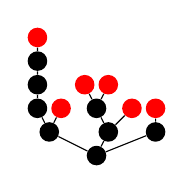
\begin{tikzpicture}[scale=.2]
\node[circle, scale=0.75, fill] (tid0) at (4.5,1.5){};
\node[circle, scale=0.75, fill] (tid1) at (1.5,3){};
\node[circle, scale=0.75, fill] (tid4) at (0.75,4.5){};
\node[circle, scale=0.75, fill] (tid9) at (0.75,6){};
\node[circle, scale=0.75, fill] (tid12) at (0.75,7.5){};
\node[circle, scale=0.75, fill, red] (tid13) at (0.75,9){};
\draw[](tid12) -- (tid13);
\draw[](tid9) -- (tid12);
\draw[](tid4) -- (tid9);
\node[circle, scale=0.75, fill, red] (tid5) at (2.25,4.5){};
\draw[](tid1) -- (tid4);
\draw[](tid1) -- (tid5);
\node[circle, scale=0.75, fill] (tid2) at (5.25,3){};
\node[circle, scale=0.75, fill] (tid6) at (4.5,4.5){};
\node[circle, scale=0.75, fill, red] (tid10) at (3.75,6){};
\node[circle, scale=0.75, fill, red] (tid11) at (5.25,6){};
\draw[](tid6) -- (tid10);
\draw[](tid6) -- (tid11);
\node[circle, scale=0.75, fill, red] (tid7) at (6.75,4.5){};
\draw[](tid2) -- (tid6);
\draw[](tid2) -- (tid7);
\node[circle, scale=0.75, fill] (tid3) at (8.25,3){};
\node[circle, scale=0.75, fill, red] (tid8) at (8.25,4.5){};
\draw[](tid3) -- (tid8);
\draw[](tid0) -- (tid1);
\draw[](tid0) -- (tid2);
\draw[](tid0) -- (tid3);
\end{tikzpicture}
\nodepart{three}
\footnotesize{6.66989}
\nodepart{four}
\footnotesize{$17\:17\:17\:33\:17$}
};
 & 
\node[draw=black, rectangle split,  rectangle split parts=4] (sn0x8a16468){
\footnotesize{14.2857}
\nodepart{two}
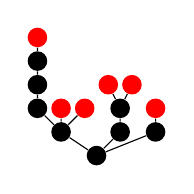
\begin{tikzpicture}[scale=.2]
\node[circle, scale=0.75, fill] (tid0) at (4.5,1.5){};
\node[circle, scale=0.75, fill] (tid1) at (2.25,3){};
\node[circle, scale=0.75, fill] (tid4) at (0.75,4.5){};
\node[circle, scale=0.75, fill] (tid9) at (0.75,6){};
\node[circle, scale=0.75, fill] (tid12) at (0.75,7.5){};
\node[circle, scale=0.75, fill, red] (tid13) at (0.75,9){};
\draw[](tid12) -- (tid13);
\draw[](tid9) -- (tid12);
\draw[](tid4) -- (tid9);
\node[circle, scale=0.75, fill, red] (tid5) at (2.25,4.5){};
\node[circle, scale=0.75, fill, red] (tid6) at (3.75,4.5){};
\draw[](tid1) -- (tid4);
\draw[](tid1) -- (tid5);
\draw[](tid1) -- (tid6);
\node[circle, scale=0.75, fill] (tid2) at (6,3){};
\node[circle, scale=0.75, fill] (tid7) at (6,4.5){};
\node[circle, scale=0.75, fill, red] (tid10) at (5.25,6){};
\node[circle, scale=0.75, fill, red] (tid11) at (6.75,6){};
\draw[](tid7) -- (tid10);
\draw[](tid7) -- (tid11);
\draw[](tid2) -- (tid7);
\node[circle, scale=0.75, fill] (tid3) at (8.25,3){};
\node[circle, scale=0.75, fill, red] (tid8) at (8.25,4.5){};
\draw[](tid3) -- (tid8);
\draw[](tid0) -- (tid1);
\draw[](tid0) -- (tid2);
\draw[](tid0) -- (tid3);
\end{tikzpicture}
\nodepart{three}
\footnotesize{6.66252}
\nodepart{four}
\footnotesize{$33\:17\:33\:17$}
};
 & 
\node[draw=black, rectangle split,  rectangle split parts=4] (sn0x8a179e8){
\footnotesize{14.2857}
\nodepart{two}
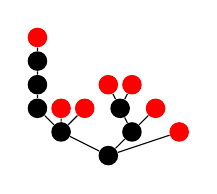
\begin{tikzpicture}[scale=.2]
\node[circle, scale=0.75, fill] (tid0) at (5.25,1.5){};
\node[circle, scale=0.75, fill] (tid1) at (2.25,3){};
\node[circle, scale=0.75, fill] (tid4) at (0.75,4.5){};
\node[circle, scale=0.75, fill] (tid9) at (0.75,6){};
\node[circle, scale=0.75, fill] (tid12) at (0.75,7.5){};
\node[circle, scale=0.75, fill, red] (tid13) at (0.75,9){};
\draw[](tid12) -- (tid13);
\draw[](tid9) -- (tid12);
\draw[](tid4) -- (tid9);
\node[circle, scale=0.75, fill, red] (tid5) at (2.25,4.5){};
\node[circle, scale=0.75, fill, red] (tid6) at (3.75,4.5){};
\draw[](tid1) -- (tid4);
\draw[](tid1) -- (tid5);
\draw[](tid1) -- (tid6);
\node[circle, scale=0.75, fill] (tid2) at (6.75,3){};
\node[circle, scale=0.75, fill] (tid7) at (6,4.5){};
\node[circle, scale=0.75, fill, red] (tid10) at (5.25,6){};
\node[circle, scale=0.75, fill, red] (tid11) at (6.75,6){};
\draw[](tid7) -- (tid10);
\draw[](tid7) -- (tid11);
\node[circle, scale=0.75, fill, red] (tid8) at (8.25,4.5){};
\draw[](tid2) -- (tid7);
\draw[](tid2) -- (tid8);
\node[circle, scale=0.75, fill, red] (tid3) at (9.75,3){};
\draw[](tid0) -- (tid1);
\draw[](tid0) -- (tid2);
\draw[](tid0) -- (tid3);
\end{tikzpicture}
\nodepart{three}
\footnotesize{6.63982}
\nodepart{four}
\footnotesize{$29\:14\:14\:29\:14$}
};
 & 
\node[draw=black, rectangle split,  rectangle split parts=4] (sn0x8a17288){
\footnotesize{28.5714}
\nodepart{two}
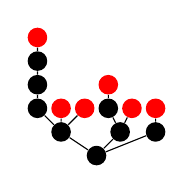
\begin{tikzpicture}[scale=.2]
\node[circle, scale=0.75, fill] (tid0) at (4.5,1.5){};
\node[circle, scale=0.75, fill] (tid1) at (2.25,3){};
\node[circle, scale=0.75, fill] (tid4) at (0.75,4.5){};
\node[circle, scale=0.75, fill] (tid10) at (0.75,6){};
\node[circle, scale=0.75, fill] (tid12) at (0.75,7.5){};
\node[circle, scale=0.75, fill, red] (tid13) at (0.75,9){};
\draw[](tid12) -- (tid13);
\draw[](tid10) -- (tid12);
\draw[](tid4) -- (tid10);
\node[circle, scale=0.75, fill, red] (tid5) at (2.25,4.5){};
\node[circle, scale=0.75, fill, red] (tid6) at (3.75,4.5){};
\draw[](tid1) -- (tid4);
\draw[](tid1) -- (tid5);
\draw[](tid1) -- (tid6);
\node[circle, scale=0.75, fill] (tid2) at (6,3){};
\node[circle, scale=0.75, fill] (tid7) at (5.25,4.5){};
\node[circle, scale=0.75, fill, red] (tid11) at (5.25,6){};
\draw[](tid7) -- (tid11);
\node[circle, scale=0.75, fill, red] (tid8) at (6.75,4.5){};
\draw[](tid2) -- (tid7);
\draw[](tid2) -- (tid8);
\node[circle, scale=0.75, fill] (tid3) at (8.25,3){};
\node[circle, scale=0.75, fill, red] (tid9) at (8.25,4.5){};
\draw[](tid3) -- (tid9);
\draw[](tid0) -- (tid1);
\draw[](tid0) -- (tid2);
\draw[](tid0) -- (tid3);
\end{tikzpicture}
\nodepart{three}
\footnotesize{6.58198}
\nodepart{four}
\footnotesize{$33\:17\:17\:17\:17$}
};
 & 
\node[draw=black, rectangle split,  rectangle split parts=4] (sn0x8a17758){
\footnotesize{14.2857}
\nodepart{two}
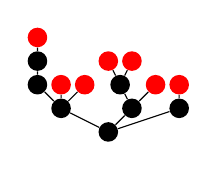
\begin{tikzpicture}[scale=.2]
\node[circle, scale=0.75, fill] (tid0) at (5.25,1.5){};
\node[circle, scale=0.75, fill] (tid1) at (2.25,3){};
\node[circle, scale=0.75, fill] (tid4) at (0.75,4.5){};
\node[circle, scale=0.75, fill] (tid10) at (0.75,6){};
\node[circle, scale=0.75, fill, red] (tid13) at (0.75,7.5){};
\draw[](tid10) -- (tid13);
\draw[](tid4) -- (tid10);
\node[circle, scale=0.75, fill, red] (tid5) at (2.25,4.5){};
\node[circle, scale=0.75, fill, red] (tid6) at (3.75,4.5){};
\draw[](tid1) -- (tid4);
\draw[](tid1) -- (tid5);
\draw[](tid1) -- (tid6);
\node[circle, scale=0.75, fill] (tid2) at (6.75,3){};
\node[circle, scale=0.75, fill] (tid7) at (6,4.5){};
\node[circle, scale=0.75, fill, red] (tid11) at (5.25,6){};
\node[circle, scale=0.75, fill, red] (tid12) at (6.75,6){};
\draw[](tid7) -- (tid11);
\draw[](tid7) -- (tid12);
\node[circle, scale=0.75, fill, red] (tid8) at (8.25,4.5){};
\draw[](tid2) -- (tid7);
\draw[](tid2) -- (tid8);
\node[circle, scale=0.75, fill] (tid3) at (9.75,3){};
\node[circle, scale=0.75, fill, red] (tid9) at (9.75,4.5){};
\draw[](tid3) -- (tid9);
\draw[](tid0) -- (tid1);
\draw[](tid0) -- (tid2);
\draw[](tid0) -- (tid3);
\end{tikzpicture}
\nodepart{three}
\footnotesize{6.09391}
\nodepart{four}
\footnotesize{$29\:14\:14\:29\:14$}
};
 & 
\\
};
\end{scope}
\begin{scope}[yshift=\leveltopIII cm]
\matrix (line3)[column sep=1cm] {
\node[draw=black, rectangle split,  rectangle split parts=4] (sn0x8a13dc0){
\footnotesize{4.76191}
\nodepart{two}
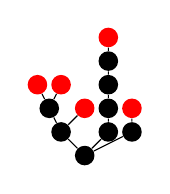
\begin{tikzpicture}[scale=.2]
\node[circle, scale=0.75, fill] (tid0) at (3.75,1.5){};
\node[circle, scale=0.75, fill] (tid1) at (2.25,3){};
\node[circle, scale=0.75, fill] (tid4) at (1.5,4.5){};
\node[circle, scale=0.75, fill, red] (tid8) at (0.75,6){};
\node[circle, scale=0.75, fill, red] (tid9) at (2.25,6){};
\draw[](tid4) -- (tid8);
\draw[](tid4) -- (tid9);
\node[circle, scale=0.75, fill, red] (tid5) at (3.75,4.5){};
\draw[](tid1) -- (tid4);
\draw[](tid1) -- (tid5);
\node[circle, scale=0.75, fill] (tid2) at (5.25,3){};
\node[circle, scale=0.75, fill] (tid6) at (5.25,4.5){};
\node[circle, scale=0.75, fill] (tid10) at (5.25,6){};
\node[circle, scale=0.75, fill] (tid11) at (5.25,7.5){};
\node[circle, scale=0.75, fill, red] (tid12) at (5.25,9){};
\draw[](tid11) -- (tid12);
\draw[](tid10) -- (tid11);
\draw[](tid6) -- (tid10);
\draw[](tid2) -- (tid6);
\node[circle, scale=0.75, fill] (tid3) at (6.75,3){};
\node[circle, scale=0.75, fill, red] (tid7) at (6.75,4.5){};
\draw[](tid3) -- (tid7);
\draw[](tid0) -- (tid1);
\draw[](tid0) -- (tid2);
\draw[](tid0) -- (tid3);
\end{tikzpicture}
\nodepart{three}
\footnotesize{6.63795}
\nodepart{four}
\footnotesize{$20\:20\:40\:20$}
};
 & 
\node[draw=black, rectangle split,  rectangle split parts=4] (sn0x8a18918){
\footnotesize{9.52381}
\nodepart{two}
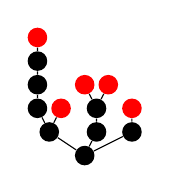
\begin{tikzpicture}[scale=.2]
\node[circle, scale=0.75, fill] (tid0) at (3.75,1.5){};
\node[circle, scale=0.75, fill] (tid1) at (1.5,3){};
\node[circle, scale=0.75, fill] (tid4) at (0.75,4.5){};
\node[circle, scale=0.75, fill] (tid8) at (0.75,6){};
\node[circle, scale=0.75, fill] (tid11) at (0.75,7.5){};
\node[circle, scale=0.75, fill, red] (tid12) at (0.75,9){};
\draw[](tid11) -- (tid12);
\draw[](tid8) -- (tid11);
\draw[](tid4) -- (tid8);
\node[circle, scale=0.75, fill, red] (tid5) at (2.25,4.5){};
\draw[](tid1) -- (tid4);
\draw[](tid1) -- (tid5);
\node[circle, scale=0.75, fill] (tid2) at (4.5,3){};
\node[circle, scale=0.75, fill] (tid6) at (4.5,4.5){};
\node[circle, scale=0.75, fill, red] (tid9) at (3.75,6){};
\node[circle, scale=0.75, fill, red] (tid10) at (5.25,6){};
\draw[](tid6) -- (tid9);
\draw[](tid6) -- (tid10);
\draw[](tid2) -- (tid6);
\node[circle, scale=0.75, fill] (tid3) at (6.75,3){};
\node[circle, scale=0.75, fill, red] (tid7) at (6.75,4.5){};
\draw[](tid3) -- (tid7);
\draw[](tid0) -- (tid1);
\draw[](tid0) -- (tid2);
\draw[](tid0) -- (tid3);
\end{tikzpicture}
\nodepart{three}
\footnotesize{6.63111}
\nodepart{four}
\footnotesize{$20\:20\:40\:20$}
};
 & 
\node[draw=black, rectangle split,  rectangle split parts=4] (sn0x8a18bd0){
\footnotesize{8.84354}
\nodepart{two}
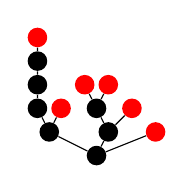
\begin{tikzpicture}[scale=.2]
\node[circle, scale=0.75, fill] (tid0) at (4.5,1.5){};
\node[circle, scale=0.75, fill] (tid1) at (1.5,3){};
\node[circle, scale=0.75, fill] (tid4) at (0.75,4.5){};
\node[circle, scale=0.75, fill] (tid8) at (0.75,6){};
\node[circle, scale=0.75, fill] (tid11) at (0.75,7.5){};
\node[circle, scale=0.75, fill, red] (tid12) at (0.75,9){};
\draw[](tid11) -- (tid12);
\draw[](tid8) -- (tid11);
\draw[](tid4) -- (tid8);
\node[circle, scale=0.75, fill, red] (tid5) at (2.25,4.5){};
\draw[](tid1) -- (tid4);
\draw[](tid1) -- (tid5);
\node[circle, scale=0.75, fill] (tid2) at (5.25,3){};
\node[circle, scale=0.75, fill] (tid6) at (4.5,4.5){};
\node[circle, scale=0.75, fill, red] (tid9) at (3.75,6){};
\node[circle, scale=0.75, fill, red] (tid10) at (5.25,6){};
\draw[](tid6) -- (tid9);
\draw[](tid6) -- (tid10);
\node[circle, scale=0.75, fill, red] (tid7) at (6.75,4.5){};
\draw[](tid2) -- (tid6);
\draw[](tid2) -- (tid7);
\node[circle, scale=0.75, fill, red] (tid3) at (8.25,3){};
\draw[](tid0) -- (tid1);
\draw[](tid0) -- (tid2);
\draw[](tid0) -- (tid3);
\end{tikzpicture}
\nodepart{three}
\footnotesize{6.60752}
\nodepart{four}
\footnotesize{$17\:17\:17\:33\:17$}
};
 & 
\node[draw=black, rectangle split,  rectangle split parts=4] (sn0x8a18e38){
\footnotesize{19.0476}
\nodepart{two}
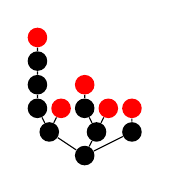
\begin{tikzpicture}[scale=.2]
\node[circle, scale=0.75, fill] (tid0) at (3.75,1.5){};
\node[circle, scale=0.75, fill] (tid1) at (1.5,3){};
\node[circle, scale=0.75, fill] (tid4) at (0.75,4.5){};
\node[circle, scale=0.75, fill] (tid9) at (0.75,6){};
\node[circle, scale=0.75, fill] (tid11) at (0.75,7.5){};
\node[circle, scale=0.75, fill, red] (tid12) at (0.75,9){};
\draw[](tid11) -- (tid12);
\draw[](tid9) -- (tid11);
\draw[](tid4) -- (tid9);
\node[circle, scale=0.75, fill, red] (tid5) at (2.25,4.5){};
\draw[](tid1) -- (tid4);
\draw[](tid1) -- (tid5);
\node[circle, scale=0.75, fill] (tid2) at (4.5,3){};
\node[circle, scale=0.75, fill] (tid6) at (3.75,4.5){};
\node[circle, scale=0.75, fill, red] (tid10) at (3.75,6){};
\draw[](tid6) -- (tid10);
\node[circle, scale=0.75, fill, red] (tid7) at (5.25,4.5){};
\draw[](tid2) -- (tid6);
\draw[](tid2) -- (tid7);
\node[circle, scale=0.75, fill] (tid3) at (6.75,3){};
\node[circle, scale=0.75, fill, red] (tid8) at (6.75,4.5){};
\draw[](tid3) -- (tid8);
\draw[](tid0) -- (tid1);
\draw[](tid0) -- (tid2);
\draw[](tid0) -- (tid3);
\end{tikzpicture}
\nodepart{three}
\footnotesize{6.54855}
\nodepart{four}
\footnotesize{$20\:20\:20\:20\:20$}
};
 & 
\node[draw=black, rectangle split,  rectangle split parts=4] (sn0x8a16b70){
\footnotesize{8.84354}
\nodepart{two}
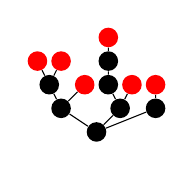
\begin{tikzpicture}[scale=.2]
\node[circle, scale=0.75, fill] (tid0) at (4.5,1.5){};
\node[circle, scale=0.75, fill] (tid1) at (2.25,3){};
\node[circle, scale=0.75, fill] (tid4) at (1.5,4.5){};
\node[circle, scale=0.75, fill, red] (tid9) at (0.75,6){};
\node[circle, scale=0.75, fill, red] (tid10) at (2.25,6){};
\draw[](tid4) -- (tid9);
\draw[](tid4) -- (tid10);
\node[circle, scale=0.75, fill, red] (tid5) at (3.75,4.5){};
\draw[](tid1) -- (tid4);
\draw[](tid1) -- (tid5);
\node[circle, scale=0.75, fill] (tid2) at (6,3){};
\node[circle, scale=0.75, fill] (tid6) at (5.25,4.5){};
\node[circle, scale=0.75, fill] (tid11) at (5.25,6){};
\node[circle, scale=0.75, fill, red] (tid12) at (5.25,7.5){};
\draw[](tid11) -- (tid12);
\draw[](tid6) -- (tid11);
\node[circle, scale=0.75, fill, red] (tid7) at (6.75,4.5){};
\draw[](tid2) -- (tid6);
\draw[](tid2) -- (tid7);
\node[circle, scale=0.75, fill] (tid3) at (8.25,3){};
\node[circle, scale=0.75, fill, red] (tid8) at (8.25,4.5){};
\draw[](tid3) -- (tid8);
\draw[](tid0) -- (tid1);
\draw[](tid0) -- (tid2);
\draw[](tid0) -- (tid3);
\end{tikzpicture}
\nodepart{three}
\footnotesize{6.04568}
\nodepart{four}
\footnotesize{$17\:17\:17\:33\:17$}
};
 & 
\node[draw=black, rectangle split,  rectangle split parts=4] (sn0x8a3d1e0){
\footnotesize{4.42177}
\nodepart{two}
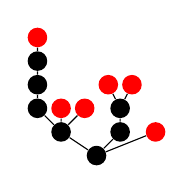
\begin{tikzpicture}[scale=.2]
\node[circle, scale=0.75, fill] (tid0) at (4.5,1.5){};
\node[circle, scale=0.75, fill] (tid1) at (2.25,3){};
\node[circle, scale=0.75, fill] (tid4) at (0.75,4.5){};
\node[circle, scale=0.75, fill] (tid8) at (0.75,6){};
\node[circle, scale=0.75, fill] (tid11) at (0.75,7.5){};
\node[circle, scale=0.75, fill, red] (tid12) at (0.75,9){};
\draw[](tid11) -- (tid12);
\draw[](tid8) -- (tid11);
\draw[](tid4) -- (tid8);
\node[circle, scale=0.75, fill, red] (tid5) at (2.25,4.5){};
\node[circle, scale=0.75, fill, red] (tid6) at (3.75,4.5){};
\draw[](tid1) -- (tid4);
\draw[](tid1) -- (tid5);
\draw[](tid1) -- (tid6);
\node[circle, scale=0.75, fill] (tid2) at (6,3){};
\node[circle, scale=0.75, fill] (tid7) at (6,4.5){};
\node[circle, scale=0.75, fill, red] (tid9) at (5.25,6){};
\node[circle, scale=0.75, fill, red] (tid10) at (6.75,6){};
\draw[](tid7) -- (tid9);
\draw[](tid7) -- (tid10);
\draw[](tid2) -- (tid7);
\node[circle, scale=0.75, fill, red] (tid3) at (8.25,3){};
\draw[](tid0) -- (tid1);
\draw[](tid0) -- (tid2);
\draw[](tid0) -- (tid3);
\end{tikzpicture}
\nodepart{three}
\footnotesize{6.59969}
\nodepart{four}
\footnotesize{$33\:17\:33\:17$}
};
 & 
\node[draw=black, rectangle split,  rectangle split parts=4] (sn0x8a3c6d8){
\footnotesize{9.52381}
\nodepart{two}
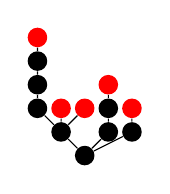
\begin{tikzpicture}[scale=.2]
\node[circle, scale=0.75, fill] (tid0) at (3.75,1.5){};
\node[circle, scale=0.75, fill] (tid1) at (2.25,3){};
\node[circle, scale=0.75, fill] (tid4) at (0.75,4.5){};
\node[circle, scale=0.75, fill] (tid9) at (0.75,6){};
\node[circle, scale=0.75, fill] (tid11) at (0.75,7.5){};
\node[circle, scale=0.75, fill, red] (tid12) at (0.75,9){};
\draw[](tid11) -- (tid12);
\draw[](tid9) -- (tid11);
\draw[](tid4) -- (tid9);
\node[circle, scale=0.75, fill, red] (tid5) at (2.25,4.5){};
\node[circle, scale=0.75, fill, red] (tid6) at (3.75,4.5){};
\draw[](tid1) -- (tid4);
\draw[](tid1) -- (tid5);
\draw[](tid1) -- (tid6);
\node[circle, scale=0.75, fill] (tid2) at (5.25,3){};
\node[circle, scale=0.75, fill] (tid7) at (5.25,4.5){};
\node[circle, scale=0.75, fill, red] (tid10) at (5.25,6){};
\draw[](tid7) -- (tid10);
\draw[](tid2) -- (tid7);
\node[circle, scale=0.75, fill] (tid3) at (6.75,3){};
\node[circle, scale=0.75, fill, red] (tid8) at (6.75,4.5){};
\draw[](tid3) -- (tid8);
\draw[](tid0) -- (tid1);
\draw[](tid0) -- (tid2);
\draw[](tid0) -- (tid3);
\end{tikzpicture}
\nodepart{three}
\footnotesize{6.53623}
\nodepart{four}
\footnotesize{$40\:20\:20\:20$}
};
 & 
\node[draw=black, rectangle split,  rectangle split parts=4] (sn0x8a3d388){
\footnotesize{4.42177}
\nodepart{two}
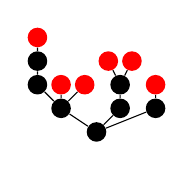
\begin{tikzpicture}[scale=.2]
\node[circle, scale=0.75, fill] (tid0) at (4.5,1.5){};
\node[circle, scale=0.75, fill] (tid1) at (2.25,3){};
\node[circle, scale=0.75, fill] (tid4) at (0.75,4.5){};
\node[circle, scale=0.75, fill] (tid9) at (0.75,6){};
\node[circle, scale=0.75, fill, red] (tid12) at (0.75,7.5){};
\draw[](tid9) -- (tid12);
\draw[](tid4) -- (tid9);
\node[circle, scale=0.75, fill, red] (tid5) at (2.25,4.5){};
\node[circle, scale=0.75, fill, red] (tid6) at (3.75,4.5){};
\draw[](tid1) -- (tid4);
\draw[](tid1) -- (tid5);
\draw[](tid1) -- (tid6);
\node[circle, scale=0.75, fill] (tid2) at (6,3){};
\node[circle, scale=0.75, fill] (tid7) at (6,4.5){};
\node[circle, scale=0.75, fill, red] (tid10) at (5.25,6){};
\node[circle, scale=0.75, fill, red] (tid11) at (6.75,6){};
\draw[](tid7) -- (tid10);
\draw[](tid7) -- (tid11);
\draw[](tid2) -- (tid7);
\node[circle, scale=0.75, fill] (tid3) at (8.25,3){};
\node[circle, scale=0.75, fill, red] (tid8) at (8.25,4.5){};
\draw[](tid3) -- (tid8);
\draw[](tid0) -- (tid1);
\draw[](tid0) -- (tid2);
\draw[](tid0) -- (tid3);
\end{tikzpicture}
\nodepart{three}
\footnotesize{6.04079}
\nodepart{four}
\footnotesize{$33\:17\:33\:17$}
};
 & 
\node[draw=black, rectangle split,  rectangle split parts=4] (sn0x8a481a8){
\footnotesize{2.04082}
\nodepart{two}
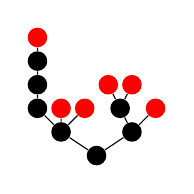
\begin{tikzpicture}[scale=.2]
\node[circle, scale=0.75, fill] (tid0) at (4.5,1.5){};
\node[circle, scale=0.75, fill] (tid1) at (2.25,3){};
\node[circle, scale=0.75, fill] (tid3) at (0.75,4.5){};
\node[circle, scale=0.75, fill] (tid8) at (0.75,6){};
\node[circle, scale=0.75, fill] (tid11) at (0.75,7.5){};
\node[circle, scale=0.75, fill, red] (tid12) at (0.75,9){};
\draw[](tid11) -- (tid12);
\draw[](tid8) -- (tid11);
\draw[](tid3) -- (tid8);
\node[circle, scale=0.75, fill, red] (tid4) at (2.25,4.5){};
\node[circle, scale=0.75, fill, red] (tid5) at (3.75,4.5){};
\draw[](tid1) -- (tid3);
\draw[](tid1) -- (tid4);
\draw[](tid1) -- (tid5);
\node[circle, scale=0.75, fill] (tid2) at (6.75,3){};
\node[circle, scale=0.75, fill] (tid6) at (6,4.5){};
\node[circle, scale=0.75, fill, red] (tid9) at (5.25,6){};
\node[circle, scale=0.75, fill, red] (tid10) at (6.75,6){};
\draw[](tid6) -- (tid9);
\draw[](tid6) -- (tid10);
\node[circle, scale=0.75, fill, red] (tid7) at (8.25,4.5){};
\draw[](tid2) -- (tid6);
\draw[](tid2) -- (tid7);
\draw[](tid0) -- (tid1);
\draw[](tid0) -- (tid2);
\end{tikzpicture}
\nodepart{three}
\footnotesize{6.6262}
\nodepart{four}
\footnotesize{$33\:17\:33\:17$}
};
 & 
\node[draw=black, rectangle split,  rectangle split parts=4] (sn0x8a49698){
\footnotesize{8.84354}
\nodepart{two}
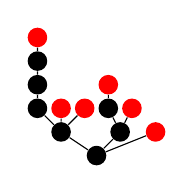
\begin{tikzpicture}[scale=.2]
\node[circle, scale=0.75, fill] (tid0) at (4.5,1.5){};
\node[circle, scale=0.75, fill] (tid1) at (2.25,3){};
\node[circle, scale=0.75, fill] (tid4) at (0.75,4.5){};
\node[circle, scale=0.75, fill] (tid9) at (0.75,6){};
\node[circle, scale=0.75, fill] (tid11) at (0.75,7.5){};
\node[circle, scale=0.75, fill, red] (tid12) at (0.75,9){};
\draw[](tid11) -- (tid12);
\draw[](tid9) -- (tid11);
\draw[](tid4) -- (tid9);
\node[circle, scale=0.75, fill, red] (tid5) at (2.25,4.5){};
\node[circle, scale=0.75, fill, red] (tid6) at (3.75,4.5){};
\draw[](tid1) -- (tid4);
\draw[](tid1) -- (tid5);
\draw[](tid1) -- (tid6);
\node[circle, scale=0.75, fill] (tid2) at (6,3){};
\node[circle, scale=0.75, fill] (tid7) at (5.25,4.5){};
\node[circle, scale=0.75, fill, red] (tid10) at (5.25,6){};
\draw[](tid7) -- (tid10);
\node[circle, scale=0.75, fill, red] (tid8) at (6.75,4.5){};
\draw[](tid2) -- (tid7);
\draw[](tid2) -- (tid8);
\node[circle, scale=0.75, fill, red] (tid3) at (8.25,3){};
\draw[](tid0) -- (tid1);
\draw[](tid0) -- (tid2);
\draw[](tid0) -- (tid3);
\end{tikzpicture}
\nodepart{three}
\footnotesize{6.51504}
\nodepart{four}
\footnotesize{$33\:17\:17\:17\:17$}
};
 & 
\node[draw=black, rectangle split,  rectangle split parts=4] (sn0x8a48da0){
\footnotesize{4.08163}
\nodepart{two}
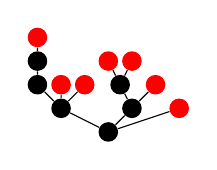
\begin{tikzpicture}[scale=.2]
\node[circle, scale=0.75, fill] (tid0) at (5.25,1.5){};
\node[circle, scale=0.75, fill] (tid1) at (2.25,3){};
\node[circle, scale=0.75, fill] (tid4) at (0.75,4.5){};
\node[circle, scale=0.75, fill] (tid9) at (0.75,6){};
\node[circle, scale=0.75, fill, red] (tid12) at (0.75,7.5){};
\draw[](tid9) -- (tid12);
\draw[](tid4) -- (tid9);
\node[circle, scale=0.75, fill, red] (tid5) at (2.25,4.5){};
\node[circle, scale=0.75, fill, red] (tid6) at (3.75,4.5){};
\draw[](tid1) -- (tid4);
\draw[](tid1) -- (tid5);
\draw[](tid1) -- (tid6);
\node[circle, scale=0.75, fill] (tid2) at (6.75,3){};
\node[circle, scale=0.75, fill] (tid7) at (6,4.5){};
\node[circle, scale=0.75, fill, red] (tid10) at (5.25,6){};
\node[circle, scale=0.75, fill, red] (tid11) at (6.75,6){};
\draw[](tid7) -- (tid10);
\draw[](tid7) -- (tid11);
\node[circle, scale=0.75, fill, red] (tid8) at (8.25,4.5){};
\draw[](tid2) -- (tid7);
\draw[](tid2) -- (tid8);
\node[circle, scale=0.75, fill, red] (tid3) at (9.75,3){};
\draw[](tid0) -- (tid1);
\draw[](tid0) -- (tid2);
\draw[](tid0) -- (tid3);
\end{tikzpicture}
\nodepart{three}
\footnotesize{6.00774}
\nodepart{four}
\footnotesize{$29\:14\:14\:29\:14$}
};
 & 
\node[draw=black, rectangle split,  rectangle split parts=4] (sn0x8a4fa48){
\footnotesize{4.76191}
\nodepart{two}
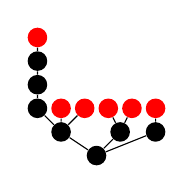
\begin{tikzpicture}[scale=.2]
\node[circle, scale=0.75, fill] (tid0) at (4.5,1.5){};
\node[circle, scale=0.75, fill] (tid1) at (2.25,3){};
\node[circle, scale=0.75, fill] (tid4) at (0.75,4.5){};
\node[circle, scale=0.75, fill] (tid10) at (0.75,6){};
\node[circle, scale=0.75, fill] (tid11) at (0.75,7.5){};
\node[circle, scale=0.75, fill, red] (tid12) at (0.75,9){};
\draw[](tid11) -- (tid12);
\draw[](tid10) -- (tid11);
\draw[](tid4) -- (tid10);
\node[circle, scale=0.75, fill, red] (tid5) at (2.25,4.5){};
\node[circle, scale=0.75, fill, red] (tid6) at (3.75,4.5){};
\draw[](tid1) -- (tid4);
\draw[](tid1) -- (tid5);
\draw[](tid1) -- (tid6);
\node[circle, scale=0.75, fill] (tid2) at (6,3){};
\node[circle, scale=0.75, fill, red] (tid7) at (5.25,4.5){};
\node[circle, scale=0.75, fill, red] (tid8) at (6.75,4.5){};
\draw[](tid2) -- (tid7);
\draw[](tid2) -- (tid8);
\node[circle, scale=0.75, fill] (tid3) at (8.25,3){};
\node[circle, scale=0.75, fill, red] (tid9) at (8.25,4.5){};
\draw[](tid3) -- (tid9);
\draw[](tid0) -- (tid1);
\draw[](tid0) -- (tid2);
\draw[](tid0) -- (tid3);
\end{tikzpicture}
\nodepart{three}
\footnotesize{6.40993}
\nodepart{four}
\footnotesize{$33\:33\:17\:17$}
};
 & 
\node[draw=black, rectangle split,  rectangle split parts=4] (sn0x8a4fb80){
\footnotesize{8.84354}
\nodepart{two}
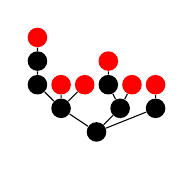
\begin{tikzpicture}[scale=.2]
\node[circle, scale=0.75, fill] (tid0) at (4.5,1.5){};
\node[circle, scale=0.75, fill] (tid1) at (2.25,3){};
\node[circle, scale=0.75, fill] (tid4) at (0.75,4.5){};
\node[circle, scale=0.75, fill] (tid10) at (0.75,6){};
\node[circle, scale=0.75, fill, red] (tid12) at (0.75,7.5){};
\draw[](tid10) -- (tid12);
\draw[](tid4) -- (tid10);
\node[circle, scale=0.75, fill, red] (tid5) at (2.25,4.5){};
\node[circle, scale=0.75, fill, red] (tid6) at (3.75,4.5){};
\draw[](tid1) -- (tid4);
\draw[](tid1) -- (tid5);
\draw[](tid1) -- (tid6);
\node[circle, scale=0.75, fill] (tid2) at (6,3){};
\node[circle, scale=0.75, fill] (tid7) at (5.25,4.5){};
\node[circle, scale=0.75, fill, red] (tid11) at (5.25,6){};
\draw[](tid7) -- (tid11);
\node[circle, scale=0.75, fill, red] (tid8) at (6.75,4.5){};
\draw[](tid2) -- (tid7);
\draw[](tid2) -- (tid8);
\node[circle, scale=0.75, fill] (tid3) at (8.25,3){};
\node[circle, scale=0.75, fill, red] (tid9) at (8.25,4.5){};
\draw[](tid3) -- (tid9);
\draw[](tid0) -- (tid1);
\draw[](tid0) -- (tid2);
\draw[](tid0) -- (tid3);
\end{tikzpicture}
\nodepart{three}
\footnotesize{5.93361}
\nodepart{four}
\footnotesize{$33\:17\:17\:17\:17$}
};
 & 
\node[draw=black, rectangle split,  rectangle split parts=4] (sn0x8a4fef8){
\footnotesize{2.04082}
\nodepart{two}
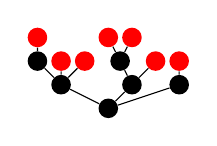
\begin{tikzpicture}[scale=.2]
\node[circle, scale=0.75, fill] (tid0) at (5.25,1.5){};
\node[circle, scale=0.75, fill] (tid1) at (2.25,3){};
\node[circle, scale=0.75, fill] (tid4) at (0.75,4.5){};
\node[circle, scale=0.75, fill, red] (tid10) at (0.75,6){};
\draw[](tid4) -- (tid10);
\node[circle, scale=0.75, fill, red] (tid5) at (2.25,4.5){};
\node[circle, scale=0.75, fill, red] (tid6) at (3.75,4.5){};
\draw[](tid1) -- (tid4);
\draw[](tid1) -- (tid5);
\draw[](tid1) -- (tid6);
\node[circle, scale=0.75, fill] (tid2) at (6.75,3){};
\node[circle, scale=0.75, fill] (tid7) at (6,4.5){};
\node[circle, scale=0.75, fill, red] (tid11) at (5.25,6){};
\node[circle, scale=0.75, fill, red] (tid12) at (6.75,6){};
\draw[](tid7) -- (tid11);
\draw[](tid7) -- (tid12);
\node[circle, scale=0.75, fill, red] (tid8) at (8.25,4.5){};
\draw[](tid2) -- (tid7);
\draw[](tid2) -- (tid8);
\node[circle, scale=0.75, fill] (tid3) at (9.75,3){};
\node[circle, scale=0.75, fill, red] (tid9) at (9.75,4.5){};
\draw[](tid3) -- (tid9);
\draw[](tid0) -- (tid1);
\draw[](tid0) -- (tid2);
\draw[](tid0) -- (tid3);
\end{tikzpicture}
\nodepart{three}
\footnotesize{5.65028}
\nodepart{four}
\footnotesize{$29\:14\:14\:29\:14$}
};
 & 
\\
};
\end{scope}
\begin{scope}[yshift=\leveltopIIII cm]
\matrix (line4)[column sep=1cm] {
\node[draw=black, rectangle split,  rectangle split parts=4] (sn0x8a19be0){
\footnotesize{2.85714}
\nodepart{two}
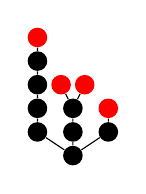
\begin{tikzpicture}[scale=.2]
\node[circle, scale=0.75, fill] (tid0) at (3,1.5){};
\node[circle, scale=0.75, fill] (tid1) at (0.75,3){};
\node[circle, scale=0.75, fill] (tid4) at (0.75,4.5){};
\node[circle, scale=0.75, fill] (tid7) at (0.75,6){};
\node[circle, scale=0.75, fill] (tid10) at (0.75,7.5){};
\node[circle, scale=0.75, fill, red] (tid11) at (0.75,9){};
\draw[](tid10) -- (tid11);
\draw[](tid7) -- (tid10);
\draw[](tid4) -- (tid7);
\draw[](tid1) -- (tid4);
\node[circle, scale=0.75, fill] (tid2) at (3,3){};
\node[circle, scale=0.75, fill] (tid5) at (3,4.5){};
\node[circle, scale=0.75, fill, red] (tid8) at (2.25,6){};
\node[circle, scale=0.75, fill, red] (tid9) at (3.75,6){};
\draw[](tid5) -- (tid8);
\draw[](tid5) -- (tid9);
\draw[](tid2) -- (tid5);
\node[circle, scale=0.75, fill] (tid3) at (5.25,3){};
\node[circle, scale=0.75, fill, red] (tid6) at (5.25,4.5){};
\draw[](tid3) -- (tid6);
\draw[](tid0) -- (tid1);
\draw[](tid0) -- (tid2);
\draw[](tid0) -- (tid3);
\end{tikzpicture}
\nodepart{three}
\footnotesize{6.59771}
\nodepart{four}
\footnotesize{$25\:50\:25$}
};
 & 
\node[draw=black, rectangle split,  rectangle split parts=4] (sn0x8a14f98){
\footnotesize{2.4263}
\nodepart{two}
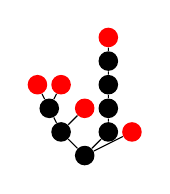
\begin{tikzpicture}[scale=.2]
\node[circle, scale=0.75, fill] (tid0) at (3.75,1.5){};
\node[circle, scale=0.75, fill] (tid1) at (2.25,3){};
\node[circle, scale=0.75, fill] (tid4) at (1.5,4.5){};
\node[circle, scale=0.75, fill, red] (tid7) at (0.75,6){};
\node[circle, scale=0.75, fill, red] (tid8) at (2.25,6){};
\draw[](tid4) -- (tid7);
\draw[](tid4) -- (tid8);
\node[circle, scale=0.75, fill, red] (tid5) at (3.75,4.5){};
\draw[](tid1) -- (tid4);
\draw[](tid1) -- (tid5);
\node[circle, scale=0.75, fill] (tid2) at (5.25,3){};
\node[circle, scale=0.75, fill] (tid6) at (5.25,4.5){};
\node[circle, scale=0.75, fill] (tid9) at (5.25,6){};
\node[circle, scale=0.75, fill] (tid10) at (5.25,7.5){};
\node[circle, scale=0.75, fill, red] (tid11) at (5.25,9){};
\draw[](tid10) -- (tid11);
\draw[](tid9) -- (tid10);
\draw[](tid6) -- (tid9);
\draw[](tid2) -- (tid6);
\node[circle, scale=0.75, fill, red] (tid3) at (6.75,3){};
\draw[](tid0) -- (tid1);
\draw[](tid0) -- (tid2);
\draw[](tid0) -- (tid3);
\end{tikzpicture}
\nodepart{three}
\footnotesize{6.57312}
\nodepart{four}
\footnotesize{$20\:20\:40\:20$}
};
 & 
\node[draw=black, rectangle split,  rectangle split parts=4] (sn0x8a18db8){
\footnotesize{5.71429}
\nodepart{two}
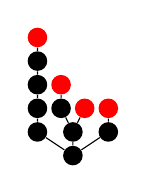
\begin{tikzpicture}[scale=.2]
\node[circle, scale=0.75, fill] (tid0) at (3,1.5){};
\node[circle, scale=0.75, fill] (tid1) at (0.75,3){};
\node[circle, scale=0.75, fill] (tid4) at (0.75,4.5){};
\node[circle, scale=0.75, fill] (tid8) at (0.75,6){};
\node[circle, scale=0.75, fill] (tid10) at (0.75,7.5){};
\node[circle, scale=0.75, fill, red] (tid11) at (0.75,9){};
\draw[](tid10) -- (tid11);
\draw[](tid8) -- (tid10);
\draw[](tid4) -- (tid8);
\draw[](tid1) -- (tid4);
\node[circle, scale=0.75, fill] (tid2) at (3,3){};
\node[circle, scale=0.75, fill] (tid5) at (2.25,4.5){};
\node[circle, scale=0.75, fill, red] (tid9) at (2.25,6){};
\draw[](tid5) -- (tid9);
\node[circle, scale=0.75, fill, red] (tid6) at (3.75,4.5){};
\draw[](tid2) -- (tid5);
\draw[](tid2) -- (tid6);
\node[circle, scale=0.75, fill] (tid3) at (5.25,3){};
\node[circle, scale=0.75, fill, red] (tid7) at (5.25,4.5){};
\draw[](tid3) -- (tid7);
\draw[](tid0) -- (tid1);
\draw[](tid0) -- (tid2);
\draw[](tid0) -- (tid3);
\end{tikzpicture}
\nodepart{three}
\footnotesize{6.51293}
\nodepart{four}
\footnotesize{$25\:25\:25\:25$}
};
 & 
\node[draw=black, rectangle split,  rectangle split parts=4] (sn0x8a1a3e0){
\footnotesize{2.4263}
\nodepart{two}
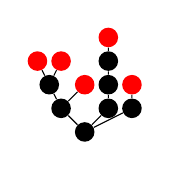
\begin{tikzpicture}[scale=.2]
\node[circle, scale=0.75, fill] (tid0) at (3.75,1.5){};
\node[circle, scale=0.75, fill] (tid1) at (2.25,3){};
\node[circle, scale=0.75, fill] (tid4) at (1.5,4.5){};
\node[circle, scale=0.75, fill, red] (tid8) at (0.75,6){};
\node[circle, scale=0.75, fill, red] (tid9) at (2.25,6){};
\draw[](tid4) -- (tid8);
\draw[](tid4) -- (tid9);
\node[circle, scale=0.75, fill, red] (tid5) at (3.75,4.5){};
\draw[](tid1) -- (tid4);
\draw[](tid1) -- (tid5);
\node[circle, scale=0.75, fill] (tid2) at (5.25,3){};
\node[circle, scale=0.75, fill] (tid6) at (5.25,4.5){};
\node[circle, scale=0.75, fill] (tid10) at (5.25,6){};
\node[circle, scale=0.75, fill, red] (tid11) at (5.25,7.5){};
\draw[](tid10) -- (tid11);
\draw[](tid6) -- (tid10);
\draw[](tid2) -- (tid6);
\node[circle, scale=0.75, fill] (tid3) at (6.75,3){};
\node[circle, scale=0.75, fill, red] (tid7) at (6.75,4.5){};
\draw[](tid3) -- (tid7);
\draw[](tid0) -- (tid1);
\draw[](tid0) -- (tid2);
\draw[](tid0) -- (tid3);
\end{tikzpicture}
\nodepart{three}
\footnotesize{5.99309}
\nodepart{four}
\footnotesize{$20\:20\:40\:20$}
};
 & 
\node[draw=black, rectangle split,  rectangle split parts=4] (sn0x8a2dc30){
\footnotesize{4.85261}
\nodepart{two}
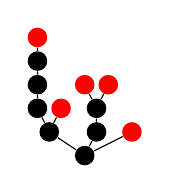
\begin{tikzpicture}[scale=.2]
\node[circle, scale=0.75, fill] (tid0) at (3.75,1.5){};
\node[circle, scale=0.75, fill] (tid1) at (1.5,3){};
\node[circle, scale=0.75, fill] (tid4) at (0.75,4.5){};
\node[circle, scale=0.75, fill] (tid7) at (0.75,6){};
\node[circle, scale=0.75, fill] (tid10) at (0.75,7.5){};
\node[circle, scale=0.75, fill, red] (tid11) at (0.75,9){};
\draw[](tid10) -- (tid11);
\draw[](tid7) -- (tid10);
\draw[](tid4) -- (tid7);
\node[circle, scale=0.75, fill, red] (tid5) at (2.25,4.5){};
\draw[](tid1) -- (tid4);
\draw[](tid1) -- (tid5);
\node[circle, scale=0.75, fill] (tid2) at (4.5,3){};
\node[circle, scale=0.75, fill] (tid6) at (4.5,4.5){};
\node[circle, scale=0.75, fill, red] (tid8) at (3.75,6){};
\node[circle, scale=0.75, fill, red] (tid9) at (5.25,6){};
\draw[](tid6) -- (tid8);
\draw[](tid6) -- (tid9);
\draw[](tid2) -- (tid6);
\node[circle, scale=0.75, fill, red] (tid3) at (6.75,3){};
\draw[](tid0) -- (tid1);
\draw[](tid0) -- (tid2);
\draw[](tid0) -- (tid3);
\end{tikzpicture}
\nodepart{three}
\footnotesize{6.56585}
\nodepart{four}
\footnotesize{$20\:20\:40\:20$}
};
 & 
\node[draw=black, rectangle split,  rectangle split parts=4] (sn0x8a2ce10){
\footnotesize{11.4286}
\nodepart{two}
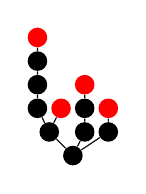
\begin{tikzpicture}[scale=.2]
\node[circle, scale=0.75, fill] (tid0) at (3,1.5){};
\node[circle, scale=0.75, fill] (tid1) at (1.5,3){};
\node[circle, scale=0.75, fill] (tid4) at (0.75,4.5){};
\node[circle, scale=0.75, fill] (tid8) at (0.75,6){};
\node[circle, scale=0.75, fill] (tid10) at (0.75,7.5){};
\node[circle, scale=0.75, fill, red] (tid11) at (0.75,9){};
\draw[](tid10) -- (tid11);
\draw[](tid8) -- (tid10);
\draw[](tid4) -- (tid8);
\node[circle, scale=0.75, fill, red] (tid5) at (2.25,4.5){};
\draw[](tid1) -- (tid4);
\draw[](tid1) -- (tid5);
\node[circle, scale=0.75, fill] (tid2) at (3.75,3){};
\node[circle, scale=0.75, fill] (tid6) at (3.75,4.5){};
\node[circle, scale=0.75, fill, red] (tid9) at (3.75,6){};
\draw[](tid6) -- (tid9);
\draw[](tid2) -- (tid6);
\node[circle, scale=0.75, fill] (tid3) at (5.25,3){};
\node[circle, scale=0.75, fill, red] (tid7) at (5.25,4.5){};
\draw[](tid3) -- (tid7);
\draw[](tid0) -- (tid1);
\draw[](tid0) -- (tid2);
\draw[](tid0) -- (tid3);
\end{tikzpicture}
\nodepart{three}
\footnotesize{6.50101}
\nodepart{four}
\footnotesize{$25\:25\:25\:25$}
};
 & 
\node[draw=black, rectangle split,  rectangle split parts=4] (sn0x8a2de40){
\footnotesize{4.85261}
\nodepart{two}
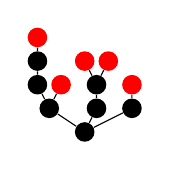
\begin{tikzpicture}[scale=.2]
\node[circle, scale=0.75, fill] (tid0) at (3.75,1.5){};
\node[circle, scale=0.75, fill] (tid1) at (1.5,3){};
\node[circle, scale=0.75, fill] (tid4) at (0.75,4.5){};
\node[circle, scale=0.75, fill] (tid8) at (0.75,6){};
\node[circle, scale=0.75, fill, red] (tid11) at (0.75,7.5){};
\draw[](tid8) -- (tid11);
\draw[](tid4) -- (tid8);
\node[circle, scale=0.75, fill, red] (tid5) at (2.25,4.5){};
\draw[](tid1) -- (tid4);
\draw[](tid1) -- (tid5);
\node[circle, scale=0.75, fill] (tid2) at (4.5,3){};
\node[circle, scale=0.75, fill] (tid6) at (4.5,4.5){};
\node[circle, scale=0.75, fill, red] (tid9) at (3.75,6){};
\node[circle, scale=0.75, fill, red] (tid10) at (5.25,6){};
\draw[](tid6) -- (tid9);
\draw[](tid6) -- (tid10);
\draw[](tid2) -- (tid6);
\node[circle, scale=0.75, fill] (tid3) at (6.75,3){};
\node[circle, scale=0.75, fill, red] (tid7) at (6.75,4.5){};
\draw[](tid3) -- (tid7);
\draw[](tid0) -- (tid1);
\draw[](tid0) -- (tid2);
\draw[](tid0) -- (tid3);
\end{tikzpicture}
\nodepart{three}
\footnotesize{5.98997}
\nodepart{four}
\footnotesize{$20\:20\:40\:20$}
};
 & 
\node[draw=black, rectangle split,  rectangle split parts=4] (sn0x8a35288){
\footnotesize{2.1542}
\nodepart{two}
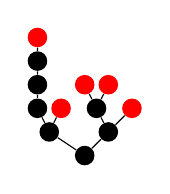
\begin{tikzpicture}[scale=.2]
\node[circle, scale=0.75, fill] (tid0) at (3.75,1.5){};
\node[circle, scale=0.75, fill] (tid1) at (1.5,3){};
\node[circle, scale=0.75, fill] (tid3) at (0.75,4.5){};
\node[circle, scale=0.75, fill] (tid7) at (0.75,6){};
\node[circle, scale=0.75, fill] (tid10) at (0.75,7.5){};
\node[circle, scale=0.75, fill, red] (tid11) at (0.75,9){};
\draw[](tid10) -- (tid11);
\draw[](tid7) -- (tid10);
\draw[](tid3) -- (tid7);
\node[circle, scale=0.75, fill, red] (tid4) at (2.25,4.5){};
\draw[](tid1) -- (tid3);
\draw[](tid1) -- (tid4);
\node[circle, scale=0.75, fill] (tid2) at (5.25,3){};
\node[circle, scale=0.75, fill] (tid5) at (4.5,4.5){};
\node[circle, scale=0.75, fill, red] (tid8) at (3.75,6){};
\node[circle, scale=0.75, fill, red] (tid9) at (5.25,6){};
\draw[](tid5) -- (tid8);
\draw[](tid5) -- (tid9);
\node[circle, scale=0.75, fill, red] (tid6) at (6.75,4.5){};
\draw[](tid2) -- (tid5);
\draw[](tid2) -- (tid6);
\draw[](tid0) -- (tid1);
\draw[](tid0) -- (tid2);
\end{tikzpicture}
\nodepart{three}
\footnotesize{6.5932}
\nodepart{four}
\footnotesize{$20\:20\:40\:20$}
};
 & 
\node[draw=black, rectangle split,  rectangle split parts=4] (sn0x8a35de8){
\footnotesize{9.70522}
\nodepart{two}
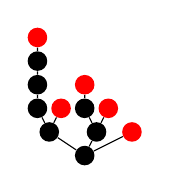
\begin{tikzpicture}[scale=.2]
\node[circle, scale=0.75, fill] (tid0) at (3.75,1.5){};
\node[circle, scale=0.75, fill] (tid1) at (1.5,3){};
\node[circle, scale=0.75, fill] (tid4) at (0.75,4.5){};
\node[circle, scale=0.75, fill] (tid8) at (0.75,6){};
\node[circle, scale=0.75, fill] (tid10) at (0.75,7.5){};
\node[circle, scale=0.75, fill, red] (tid11) at (0.75,9){};
\draw[](tid10) -- (tid11);
\draw[](tid8) -- (tid10);
\draw[](tid4) -- (tid8);
\node[circle, scale=0.75, fill, red] (tid5) at (2.25,4.5){};
\draw[](tid1) -- (tid4);
\draw[](tid1) -- (tid5);
\node[circle, scale=0.75, fill] (tid2) at (4.5,3){};
\node[circle, scale=0.75, fill] (tid6) at (3.75,4.5){};
\node[circle, scale=0.75, fill, red] (tid9) at (3.75,6){};
\draw[](tid6) -- (tid9);
\node[circle, scale=0.75, fill, red] (tid7) at (5.25,4.5){};
\draw[](tid2) -- (tid6);
\draw[](tid2) -- (tid7);
\node[circle, scale=0.75, fill, red] (tid3) at (6.75,3){};
\draw[](tid0) -- (tid1);
\draw[](tid0) -- (tid2);
\draw[](tid0) -- (tid3);
\end{tikzpicture}
\nodepart{three}
\footnotesize{6.4789}
\nodepart{four}
\footnotesize{$20\:20\:20\:20\:20$}
};
 & 
\node[draw=black, rectangle split,  rectangle split parts=4] (sn0x8a35350){
\footnotesize{4.11403}
\nodepart{two}
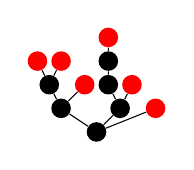
\begin{tikzpicture}[scale=.2]
\node[circle, scale=0.75, fill] (tid0) at (4.5,1.5){};
\node[circle, scale=0.75, fill] (tid1) at (2.25,3){};
\node[circle, scale=0.75, fill] (tid4) at (1.5,4.5){};
\node[circle, scale=0.75, fill, red] (tid8) at (0.75,6){};
\node[circle, scale=0.75, fill, red] (tid9) at (2.25,6){};
\draw[](tid4) -- (tid8);
\draw[](tid4) -- (tid9);
\node[circle, scale=0.75, fill, red] (tid5) at (3.75,4.5){};
\draw[](tid1) -- (tid4);
\draw[](tid1) -- (tid5);
\node[circle, scale=0.75, fill] (tid2) at (6,3){};
\node[circle, scale=0.75, fill] (tid6) at (5.25,4.5){};
\node[circle, scale=0.75, fill] (tid10) at (5.25,6){};
\node[circle, scale=0.75, fill, red] (tid11) at (5.25,7.5){};
\draw[](tid10) -- (tid11);
\draw[](tid6) -- (tid10);
\node[circle, scale=0.75, fill, red] (tid7) at (6.75,4.5){};
\draw[](tid2) -- (tid6);
\draw[](tid2) -- (tid7);
\node[circle, scale=0.75, fill, red] (tid3) at (8.25,3){};
\draw[](tid0) -- (tid1);
\draw[](tid0) -- (tid2);
\draw[](tid0) -- (tid3);
\end{tikzpicture}
\nodepart{three}
\footnotesize{5.95514}
\nodepart{four}
\footnotesize{$17\:17\:17\:33\:17$}
};
 & 
\node[draw=black, rectangle split,  rectangle split parts=4] (sn0x8a3ac00){
\footnotesize{5.39683}
\nodepart{two}
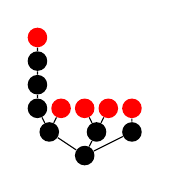
\begin{tikzpicture}[scale=.2]
\node[circle, scale=0.75, fill] (tid0) at (3.75,1.5){};
\node[circle, scale=0.75, fill] (tid1) at (1.5,3){};
\node[circle, scale=0.75, fill] (tid4) at (0.75,4.5){};
\node[circle, scale=0.75, fill] (tid9) at (0.75,6){};
\node[circle, scale=0.75, fill] (tid10) at (0.75,7.5){};
\node[circle, scale=0.75, fill, red] (tid11) at (0.75,9){};
\draw[](tid10) -- (tid11);
\draw[](tid9) -- (tid10);
\draw[](tid4) -- (tid9);
\node[circle, scale=0.75, fill, red] (tid5) at (2.25,4.5){};
\draw[](tid1) -- (tid4);
\draw[](tid1) -- (tid5);
\node[circle, scale=0.75, fill] (tid2) at (4.5,3){};
\node[circle, scale=0.75, fill, red] (tid6) at (3.75,4.5){};
\node[circle, scale=0.75, fill, red] (tid7) at (5.25,4.5){};
\draw[](tid2) -- (tid6);
\draw[](tid2) -- (tid7);
\node[circle, scale=0.75, fill] (tid3) at (6.75,3){};
\node[circle, scale=0.75, fill, red] (tid8) at (6.75,4.5){};
\draw[](tid3) -- (tid8);
\draw[](tid0) -- (tid1);
\draw[](tid0) -- (tid2);
\draw[](tid0) -- (tid3);
\end{tikzpicture}
\nodepart{three}
\footnotesize{6.37091}
\nodepart{four}
\footnotesize{$20\:40\:20\:20$}
};
 & 
\node[draw=black, rectangle split,  rectangle split parts=4] (sn0x8a39720){
\footnotesize{9.70522}
\nodepart{two}
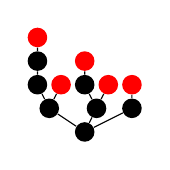
\begin{tikzpicture}[scale=.2]
\node[circle, scale=0.75, fill] (tid0) at (3.75,1.5){};
\node[circle, scale=0.75, fill] (tid1) at (1.5,3){};
\node[circle, scale=0.75, fill] (tid4) at (0.75,4.5){};
\node[circle, scale=0.75, fill] (tid9) at (0.75,6){};
\node[circle, scale=0.75, fill, red] (tid11) at (0.75,7.5){};
\draw[](tid9) -- (tid11);
\draw[](tid4) -- (tid9);
\node[circle, scale=0.75, fill, red] (tid5) at (2.25,4.5){};
\draw[](tid1) -- (tid4);
\draw[](tid1) -- (tid5);
\node[circle, scale=0.75, fill] (tid2) at (4.5,3){};
\node[circle, scale=0.75, fill] (tid6) at (3.75,4.5){};
\node[circle, scale=0.75, fill, red] (tid10) at (3.75,6){};
\draw[](tid6) -- (tid10);
\node[circle, scale=0.75, fill, red] (tid7) at (5.25,4.5){};
\draw[](tid2) -- (tid6);
\draw[](tid2) -- (tid7);
\node[circle, scale=0.75, fill] (tid3) at (6.75,3){};
\node[circle, scale=0.75, fill, red] (tid8) at (6.75,4.5){};
\draw[](tid3) -- (tid8);
\draw[](tid0) -- (tid1);
\draw[](tid0) -- (tid2);
\draw[](tid0) -- (tid3);
\end{tikzpicture}
\nodepart{three}
\footnotesize{5.87901}
\nodepart{four}
\footnotesize{$20\:20\:20\:20\:20$}
};
 & 
\node[draw=black, rectangle split,  rectangle split parts=4] (sn0x8a3b428){
\footnotesize{2.05701}
\nodepart{two}
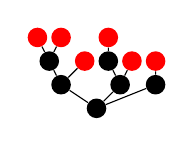
\begin{tikzpicture}[scale=.2]
\node[circle, scale=0.75, fill] (tid0) at (4.5,1.5){};
\node[circle, scale=0.75, fill] (tid1) at (2.25,3){};
\node[circle, scale=0.75, fill] (tid4) at (1.5,4.5){};
\node[circle, scale=0.75, fill, red] (tid9) at (0.75,6){};
\node[circle, scale=0.75, fill, red] (tid10) at (2.25,6){};
\draw[](tid4) -- (tid9);
\draw[](tid4) -- (tid10);
\node[circle, scale=0.75, fill, red] (tid5) at (3.75,4.5){};
\draw[](tid1) -- (tid4);
\draw[](tid1) -- (tid5);
\node[circle, scale=0.75, fill] (tid2) at (6,3){};
\node[circle, scale=0.75, fill] (tid6) at (5.25,4.5){};
\node[circle, scale=0.75, fill, red] (tid11) at (5.25,6){};
\draw[](tid6) -- (tid11);
\node[circle, scale=0.75, fill, red] (tid7) at (6.75,4.5){};
\draw[](tid2) -- (tid6);
\draw[](tid2) -- (tid7);
\node[circle, scale=0.75, fill] (tid3) at (8.25,3){};
\node[circle, scale=0.75, fill, red] (tid8) at (8.25,4.5){};
\draw[](tid3) -- (tid8);
\draw[](tid0) -- (tid1);
\draw[](tid0) -- (tid2);
\draw[](tid0) -- (tid3);
\end{tikzpicture}
\nodepart{three}
\footnotesize{5.57786}
\nodepart{four}
\footnotesize{$17\:17\:17\:33\:17$}
};
 & 
\node[draw=black, rectangle split,  rectangle split parts=4] (sn0x8a3c530){
\footnotesize{1.0771}
\nodepart{two}
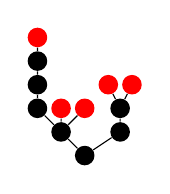
\begin{tikzpicture}[scale=.2]
\node[circle, scale=0.75, fill] (tid0) at (3.75,1.5){};
\node[circle, scale=0.75, fill] (tid1) at (2.25,3){};
\node[circle, scale=0.75, fill] (tid3) at (0.75,4.5){};
\node[circle, scale=0.75, fill] (tid7) at (0.75,6){};
\node[circle, scale=0.75, fill] (tid10) at (0.75,7.5){};
\node[circle, scale=0.75, fill, red] (tid11) at (0.75,9){};
\draw[](tid10) -- (tid11);
\draw[](tid7) -- (tid10);
\draw[](tid3) -- (tid7);
\node[circle, scale=0.75, fill, red] (tid4) at (2.25,4.5){};
\node[circle, scale=0.75, fill, red] (tid5) at (3.75,4.5){};
\draw[](tid1) -- (tid3);
\draw[](tid1) -- (tid4);
\draw[](tid1) -- (tid5);
\node[circle, scale=0.75, fill] (tid2) at (6,3){};
\node[circle, scale=0.75, fill] (tid6) at (6,4.5){};
\node[circle, scale=0.75, fill, red] (tid8) at (5.25,6){};
\node[circle, scale=0.75, fill, red] (tid9) at (6.75,6){};
\draw[](tid6) -- (tid8);
\draw[](tid6) -- (tid9);
\draw[](tid2) -- (tid6);
\draw[](tid0) -- (tid1);
\draw[](tid0) -- (tid2);
\end{tikzpicture}
\nodepart{three}
\footnotesize{6.58523}
\nodepart{four}
\footnotesize{$40\:40\:20$}
};
 & 
\node[draw=black, rectangle split,  rectangle split parts=4] (sn0x8a3dad0){
\footnotesize{4.85261}
\nodepart{two}
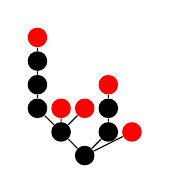
\begin{tikzpicture}[scale=.2]
\node[circle, scale=0.75, fill] (tid0) at (3.75,1.5){};
\node[circle, scale=0.75, fill] (tid1) at (2.25,3){};
\node[circle, scale=0.75, fill] (tid4) at (0.75,4.5){};
\node[circle, scale=0.75, fill] (tid8) at (0.75,6){};
\node[circle, scale=0.75, fill] (tid10) at (0.75,7.5){};
\node[circle, scale=0.75, fill, red] (tid11) at (0.75,9){};
\draw[](tid10) -- (tid11);
\draw[](tid8) -- (tid10);
\draw[](tid4) -- (tid8);
\node[circle, scale=0.75, fill, red] (tid5) at (2.25,4.5){};
\node[circle, scale=0.75, fill, red] (tid6) at (3.75,4.5){};
\draw[](tid1) -- (tid4);
\draw[](tid1) -- (tid5);
\draw[](tid1) -- (tid6);
\node[circle, scale=0.75, fill] (tid2) at (5.25,3){};
\node[circle, scale=0.75, fill] (tid7) at (5.25,4.5){};
\node[circle, scale=0.75, fill, red] (tid9) at (5.25,6){};
\draw[](tid7) -- (tid9);
\draw[](tid2) -- (tid7);
\node[circle, scale=0.75, fill, red] (tid3) at (6.75,3){};
\draw[](tid0) -- (tid1);
\draw[](tid0) -- (tid2);
\draw[](tid0) -- (tid3);
\end{tikzpicture}
\nodepart{three}
\footnotesize{6.46567}
\nodepart{four}
\footnotesize{$40\:20\:20\:20$}
};
 & 
\node[draw=black, rectangle split,  rectangle split parts=4] (sn0x8a3cc68){
\footnotesize{2.05701}
\nodepart{two}
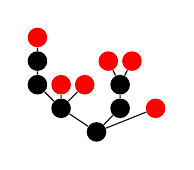
\begin{tikzpicture}[scale=.2]
\node[circle, scale=0.75, fill] (tid0) at (4.5,1.5){};
\node[circle, scale=0.75, fill] (tid1) at (2.25,3){};
\node[circle, scale=0.75, fill] (tid4) at (0.75,4.5){};
\node[circle, scale=0.75, fill] (tid8) at (0.75,6){};
\node[circle, scale=0.75, fill, red] (tid11) at (0.75,7.5){};
\draw[](tid8) -- (tid11);
\draw[](tid4) -- (tid8);
\node[circle, scale=0.75, fill, red] (tid5) at (2.25,4.5){};
\node[circle, scale=0.75, fill, red] (tid6) at (3.75,4.5){};
\draw[](tid1) -- (tid4);
\draw[](tid1) -- (tid5);
\draw[](tid1) -- (tid6);
\node[circle, scale=0.75, fill] (tid2) at (6,3){};
\node[circle, scale=0.75, fill] (tid7) at (6,4.5){};
\node[circle, scale=0.75, fill, red] (tid9) at (5.25,6){};
\node[circle, scale=0.75, fill, red] (tid10) at (6.75,6){};
\draw[](tid7) -- (tid9);
\draw[](tid7) -- (tid10);
\draw[](tid2) -- (tid7);
\node[circle, scale=0.75, fill, red] (tid3) at (8.25,3){};
\draw[](tid0) -- (tid1);
\draw[](tid0) -- (tid2);
\draw[](tid0) -- (tid3);
\end{tikzpicture}
\nodepart{three}
\footnotesize{5.94985}
\nodepart{four}
\footnotesize{$33\:17\:33\:17$}
};
 & 
\node[draw=black, rectangle split,  rectangle split parts=4] (sn0x8a45480){
\footnotesize{3.49206}
\nodepart{two}
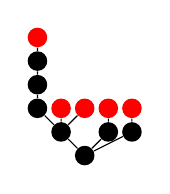
\begin{tikzpicture}[scale=.2]
\node[circle, scale=0.75, fill] (tid0) at (3.75,1.5){};
\node[circle, scale=0.75, fill] (tid1) at (2.25,3){};
\node[circle, scale=0.75, fill] (tid4) at (0.75,4.5){};
\node[circle, scale=0.75, fill] (tid9) at (0.75,6){};
\node[circle, scale=0.75, fill] (tid10) at (0.75,7.5){};
\node[circle, scale=0.75, fill, red] (tid11) at (0.75,9){};
\draw[](tid10) -- (tid11);
\draw[](tid9) -- (tid10);
\draw[](tid4) -- (tid9);
\node[circle, scale=0.75, fill, red] (tid5) at (2.25,4.5){};
\node[circle, scale=0.75, fill, red] (tid6) at (3.75,4.5){};
\draw[](tid1) -- (tid4);
\draw[](tid1) -- (tid5);
\draw[](tid1) -- (tid6);
\node[circle, scale=0.75, fill] (tid2) at (5.25,3){};
\node[circle, scale=0.75, fill, red] (tid7) at (5.25,4.5){};
\draw[](tid2) -- (tid7);
\node[circle, scale=0.75, fill] (tid3) at (6.75,3){};
\node[circle, scale=0.75, fill, red] (tid8) at (6.75,4.5){};
\draw[](tid3) -- (tid8);
\draw[](tid0) -- (tid1);
\draw[](tid0) -- (tid2);
\draw[](tid0) -- (tid3);
\end{tikzpicture}
\nodepart{three}
\footnotesize{6.3461}
\nodepart{four}
\footnotesize{$40\:40\:20$}
};
 & 
\node[draw=black, rectangle split,  rectangle split parts=4] (sn0x8a44d68){
\footnotesize{4.85261}
\nodepart{two}
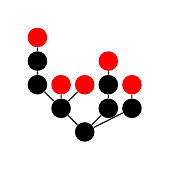
\begin{tikzpicture}[scale=.2]
\node[circle, scale=0.75, fill] (tid0) at (3.75,1.5){};
\node[circle, scale=0.75, fill] (tid1) at (2.25,3){};
\node[circle, scale=0.75, fill] (tid4) at (0.75,4.5){};
\node[circle, scale=0.75, fill] (tid9) at (0.75,6){};
\node[circle, scale=0.75, fill, red] (tid11) at (0.75,7.5){};
\draw[](tid9) -- (tid11);
\draw[](tid4) -- (tid9);
\node[circle, scale=0.75, fill, red] (tid5) at (2.25,4.5){};
\node[circle, scale=0.75, fill, red] (tid6) at (3.75,4.5){};
\draw[](tid1) -- (tid4);
\draw[](tid1) -- (tid5);
\draw[](tid1) -- (tid6);
\node[circle, scale=0.75, fill] (tid2) at (5.25,3){};
\node[circle, scale=0.75, fill] (tid7) at (5.25,4.5){};
\node[circle, scale=0.75, fill, red] (tid10) at (5.25,6){};
\draw[](tid7) -- (tid10);
\draw[](tid2) -- (tid7);
\node[circle, scale=0.75, fill] (tid3) at (6.75,3){};
\node[circle, scale=0.75, fill, red] (tid8) at (6.75,4.5){};
\draw[](tid3) -- (tid8);
\draw[](tid0) -- (tid1);
\draw[](tid0) -- (tid2);
\draw[](tid0) -- (tid3);
\end{tikzpicture}
\nodepart{three}
\footnotesize{5.86734}
\nodepart{four}
\footnotesize{$40\:20\:20\:20$}
};
 & 
\node[draw=black, rectangle split,  rectangle split parts=4] (sn0x8a48500){
\footnotesize{1.02851}
\nodepart{two}
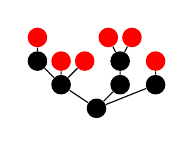
\begin{tikzpicture}[scale=.2]
\node[circle, scale=0.75, fill] (tid0) at (4.5,1.5){};
\node[circle, scale=0.75, fill] (tid1) at (2.25,3){};
\node[circle, scale=0.75, fill] (tid4) at (0.75,4.5){};
\node[circle, scale=0.75, fill, red] (tid9) at (0.75,6){};
\draw[](tid4) -- (tid9);
\node[circle, scale=0.75, fill, red] (tid5) at (2.25,4.5){};
\node[circle, scale=0.75, fill, red] (tid6) at (3.75,4.5){};
\draw[](tid1) -- (tid4);
\draw[](tid1) -- (tid5);
\draw[](tid1) -- (tid6);
\node[circle, scale=0.75, fill] (tid2) at (6,3){};
\node[circle, scale=0.75, fill] (tid7) at (6,4.5){};
\node[circle, scale=0.75, fill, red] (tid10) at (5.25,6){};
\node[circle, scale=0.75, fill, red] (tid11) at (6.75,6){};
\draw[](tid7) -- (tid10);
\draw[](tid7) -- (tid11);
\draw[](tid2) -- (tid7);
\node[circle, scale=0.75, fill] (tid3) at (8.25,3){};
\node[circle, scale=0.75, fill, red] (tid8) at (8.25,4.5){};
\draw[](tid3) -- (tid8);
\draw[](tid0) -- (tid1);
\draw[](tid0) -- (tid2);
\draw[](tid0) -- (tid3);
\end{tikzpicture}
\nodepart{three}
\footnotesize{5.58027}
\nodepart{four}
\footnotesize{$33\:17\:33\:17$}
};
 & 
\node[draw=black, rectangle split,  rectangle split parts=4] (sn0x8a49768){
\footnotesize{2.1542}
\nodepart{two}
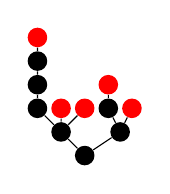
\begin{tikzpicture}[scale=.2]
\node[circle, scale=0.75, fill] (tid0) at (3.75,1.5){};
\node[circle, scale=0.75, fill] (tid1) at (2.25,3){};
\node[circle, scale=0.75, fill] (tid3) at (0.75,4.5){};
\node[circle, scale=0.75, fill] (tid8) at (0.75,6){};
\node[circle, scale=0.75, fill] (tid10) at (0.75,7.5){};
\node[circle, scale=0.75, fill, red] (tid11) at (0.75,9){};
\draw[](tid10) -- (tid11);
\draw[](tid8) -- (tid10);
\draw[](tid3) -- (tid8);
\node[circle, scale=0.75, fill, red] (tid4) at (2.25,4.5){};
\node[circle, scale=0.75, fill, red] (tid5) at (3.75,4.5){};
\draw[](tid1) -- (tid3);
\draw[](tid1) -- (tid4);
\draw[](tid1) -- (tid5);
\node[circle, scale=0.75, fill] (tid2) at (6,3){};
\node[circle, scale=0.75, fill] (tid6) at (5.25,4.5){};
\node[circle, scale=0.75, fill, red] (tid9) at (5.25,6){};
\draw[](tid6) -- (tid9);
\node[circle, scale=0.75, fill, red] (tid7) at (6.75,4.5){};
\draw[](tid2) -- (tid6);
\draw[](tid2) -- (tid7);
\draw[](tid0) -- (tid1);
\draw[](tid0) -- (tid2);
\end{tikzpicture}
\nodepart{three}
\footnotesize{6.49941}
\nodepart{four}
\footnotesize{$40\:20\:20\:20$}
};
 & 
\node[draw=black, rectangle split,  rectangle split parts=4] (sn0x8a48640){
\footnotesize{0.923226}
\nodepart{two}
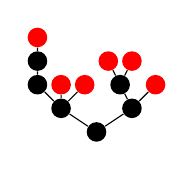
\begin{tikzpicture}[scale=.2]
\node[circle, scale=0.75, fill] (tid0) at (4.5,1.5){};
\node[circle, scale=0.75, fill] (tid1) at (2.25,3){};
\node[circle, scale=0.75, fill] (tid3) at (0.75,4.5){};
\node[circle, scale=0.75, fill] (tid8) at (0.75,6){};
\node[circle, scale=0.75, fill, red] (tid11) at (0.75,7.5){};
\draw[](tid8) -- (tid11);
\draw[](tid3) -- (tid8);
\node[circle, scale=0.75, fill, red] (tid4) at (2.25,4.5){};
\node[circle, scale=0.75, fill, red] (tid5) at (3.75,4.5){};
\draw[](tid1) -- (tid3);
\draw[](tid1) -- (tid4);
\draw[](tid1) -- (tid5);
\node[circle, scale=0.75, fill] (tid2) at (6.75,3){};
\node[circle, scale=0.75, fill] (tid6) at (6,4.5){};
\node[circle, scale=0.75, fill, red] (tid9) at (5.25,6){};
\node[circle, scale=0.75, fill, red] (tid10) at (6.75,6){};
\draw[](tid6) -- (tid9);
\draw[](tid6) -- (tid10);
\node[circle, scale=0.75, fill, red] (tid7) at (8.25,4.5){};
\draw[](tid2) -- (tid6);
\draw[](tid2) -- (tid7);
\draw[](tid0) -- (tid1);
\draw[](tid0) -- (tid2);
\end{tikzpicture}
\nodepart{three}
\footnotesize{5.98673}
\nodepart{four}
\footnotesize{$33\:17\:33\:17$}
};
 & 
\node[draw=black, rectangle split,  rectangle split parts=4] (sn0x8a4cf38){
\footnotesize{2.26757}
\nodepart{two}
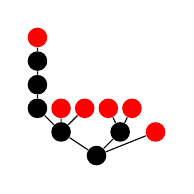
\begin{tikzpicture}[scale=.2]
\node[circle, scale=0.75, fill] (tid0) at (4.5,1.5){};
\node[circle, scale=0.75, fill] (tid1) at (2.25,3){};
\node[circle, scale=0.75, fill] (tid4) at (0.75,4.5){};
\node[circle, scale=0.75, fill] (tid9) at (0.75,6){};
\node[circle, scale=0.75, fill] (tid10) at (0.75,7.5){};
\node[circle, scale=0.75, fill, red] (tid11) at (0.75,9){};
\draw[](tid10) -- (tid11);
\draw[](tid9) -- (tid10);
\draw[](tid4) -- (tid9);
\node[circle, scale=0.75, fill, red] (tid5) at (2.25,4.5){};
\node[circle, scale=0.75, fill, red] (tid6) at (3.75,4.5){};
\draw[](tid1) -- (tid4);
\draw[](tid1) -- (tid5);
\draw[](tid1) -- (tid6);
\node[circle, scale=0.75, fill] (tid2) at (6,3){};
\node[circle, scale=0.75, fill, red] (tid7) at (5.25,4.5){};
\node[circle, scale=0.75, fill, red] (tid8) at (6.75,4.5){};
\draw[](tid2) -- (tid7);
\draw[](tid2) -- (tid8);
\node[circle, scale=0.75, fill, red] (tid3) at (8.25,3){};
\draw[](tid0) -- (tid1);
\draw[](tid0) -- (tid2);
\draw[](tid0) -- (tid3);
\end{tikzpicture}
\nodepart{three}
\footnotesize{6.33165}
\nodepart{four}
\footnotesize{$33\:33\:17\:17$}
};
 & 
\node[draw=black, rectangle split,  rectangle split parts=4] (sn0x8a4c570){
\footnotesize{4.11403}
\nodepart{two}
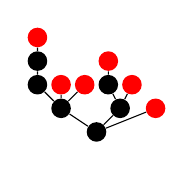
\begin{tikzpicture}[scale=.2]
\node[circle, scale=0.75, fill] (tid0) at (4.5,1.5){};
\node[circle, scale=0.75, fill] (tid1) at (2.25,3){};
\node[circle, scale=0.75, fill] (tid4) at (0.75,4.5){};
\node[circle, scale=0.75, fill] (tid9) at (0.75,6){};
\node[circle, scale=0.75, fill, red] (tid11) at (0.75,7.5){};
\draw[](tid9) -- (tid11);
\draw[](tid4) -- (tid9);
\node[circle, scale=0.75, fill, red] (tid5) at (2.25,4.5){};
\node[circle, scale=0.75, fill, red] (tid6) at (3.75,4.5){};
\draw[](tid1) -- (tid4);
\draw[](tid1) -- (tid5);
\draw[](tid1) -- (tid6);
\node[circle, scale=0.75, fill] (tid2) at (6,3){};
\node[circle, scale=0.75, fill] (tid7) at (5.25,4.5){};
\node[circle, scale=0.75, fill, red] (tid10) at (5.25,6){};
\draw[](tid7) -- (tid10);
\node[circle, scale=0.75, fill, red] (tid8) at (6.75,4.5){};
\draw[](tid2) -- (tid7);
\draw[](tid2) -- (tid8);
\node[circle, scale=0.75, fill, red] (tid3) at (8.25,3){};
\draw[](tid0) -- (tid1);
\draw[](tid0) -- (tid2);
\draw[](tid0) -- (tid3);
\end{tikzpicture}
\nodepart{three}
\footnotesize{5.83574}
\nodepart{four}
\footnotesize{$33\:17\:17\:17\:17$}
};
 & 
\node[draw=black, rectangle split,  rectangle split parts=4] (sn0x8a4e2f0){
\footnotesize{0.874636}
\nodepart{two}
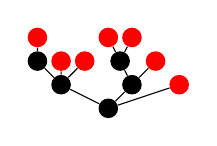
\begin{tikzpicture}[scale=.2]
\node[circle, scale=0.75, fill] (tid0) at (5.25,1.5){};
\node[circle, scale=0.75, fill] (tid1) at (2.25,3){};
\node[circle, scale=0.75, fill] (tid4) at (0.75,4.5){};
\node[circle, scale=0.75, fill, red] (tid9) at (0.75,6){};
\draw[](tid4) -- (tid9);
\node[circle, scale=0.75, fill, red] (tid5) at (2.25,4.5){};
\node[circle, scale=0.75, fill, red] (tid6) at (3.75,4.5){};
\draw[](tid1) -- (tid4);
\draw[](tid1) -- (tid5);
\draw[](tid1) -- (tid6);
\node[circle, scale=0.75, fill] (tid2) at (6.75,3){};
\node[circle, scale=0.75, fill] (tid7) at (6,4.5){};
\node[circle, scale=0.75, fill, red] (tid10) at (5.25,6){};
\node[circle, scale=0.75, fill, red] (tid11) at (6.75,6){};
\draw[](tid7) -- (tid10);
\draw[](tid7) -- (tid11);
\node[circle, scale=0.75, fill, red] (tid8) at (8.25,4.5){};
\draw[](tid2) -- (tid7);
\draw[](tid2) -- (tid8);
\node[circle, scale=0.75, fill, red] (tid3) at (9.75,3){};
\draw[](tid0) -- (tid1);
\draw[](tid0) -- (tid2);
\draw[](tid0) -- (tid3);
\end{tikzpicture}
\nodepart{three}
\footnotesize{5.53581}
\nodepart{four}
\footnotesize{$29\:14\:14\:29\:14$}
};
 & 
\node[draw=black, rectangle split,  rectangle split parts=4] (sn0x8a50558){
\footnotesize{2.26757}
\nodepart{two}
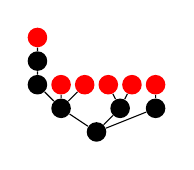
\begin{tikzpicture}[scale=.2]
\node[circle, scale=0.75, fill] (tid0) at (4.5,1.5){};
\node[circle, scale=0.75, fill] (tid1) at (2.25,3){};
\node[circle, scale=0.75, fill] (tid4) at (0.75,4.5){};
\node[circle, scale=0.75, fill] (tid10) at (0.75,6){};
\node[circle, scale=0.75, fill, red] (tid11) at (0.75,7.5){};
\draw[](tid10) -- (tid11);
\draw[](tid4) -- (tid10);
\node[circle, scale=0.75, fill, red] (tid5) at (2.25,4.5){};
\node[circle, scale=0.75, fill, red] (tid6) at (3.75,4.5){};
\draw[](tid1) -- (tid4);
\draw[](tid1) -- (tid5);
\draw[](tid1) -- (tid6);
\node[circle, scale=0.75, fill] (tid2) at (6,3){};
\node[circle, scale=0.75, fill, red] (tid7) at (5.25,4.5){};
\node[circle, scale=0.75, fill, red] (tid8) at (6.75,4.5){};
\draw[](tid2) -- (tid7);
\draw[](tid2) -- (tid8);
\node[circle, scale=0.75, fill] (tid3) at (8.25,3){};
\node[circle, scale=0.75, fill, red] (tid9) at (8.25,4.5){};
\draw[](tid3) -- (tid9);
\draw[](tid0) -- (tid1);
\draw[](tid0) -- (tid2);
\draw[](tid0) -- (tid3);
\end{tikzpicture}
\nodepart{three}
\footnotesize{5.69389}
\nodepart{four}
\footnotesize{$33\:33\:17\:17$}
};
 & 
\node[draw=black, rectangle split,  rectangle split parts=4] (sn0x8a50e60){
\footnotesize{2.05701}
\nodepart{two}
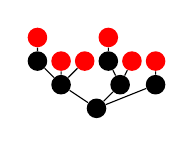
\begin{tikzpicture}[scale=.2]
\node[circle, scale=0.75, fill] (tid0) at (4.5,1.5){};
\node[circle, scale=0.75, fill] (tid1) at (2.25,3){};
\node[circle, scale=0.75, fill] (tid4) at (0.75,4.5){};
\node[circle, scale=0.75, fill, red] (tid10) at (0.75,6){};
\draw[](tid4) -- (tid10);
\node[circle, scale=0.75, fill, red] (tid5) at (2.25,4.5){};
\node[circle, scale=0.75, fill, red] (tid6) at (3.75,4.5){};
\draw[](tid1) -- (tid4);
\draw[](tid1) -- (tid5);
\draw[](tid1) -- (tid6);
\node[circle, scale=0.75, fill] (tid2) at (6,3){};
\node[circle, scale=0.75, fill] (tid7) at (5.25,4.5){};
\node[circle, scale=0.75, fill, red] (tid11) at (5.25,6){};
\draw[](tid7) -- (tid11);
\node[circle, scale=0.75, fill, red] (tid8) at (6.75,4.5){};
\draw[](tid2) -- (tid7);
\draw[](tid2) -- (tid8);
\node[circle, scale=0.75, fill] (tid3) at (8.25,3){};
\node[circle, scale=0.75, fill, red] (tid9) at (8.25,4.5){};
\draw[](tid3) -- (tid9);
\draw[](tid0) -- (tid1);
\draw[](tid0) -- (tid2);
\draw[](tid0) -- (tid3);
\end{tikzpicture}
\nodepart{three}
\footnotesize{5.44666}
\nodepart{four}
\footnotesize{$33\:17\:17\:17\:17$}
};
 & 
\node[draw=black, rectangle split,  rectangle split parts=4] (sn0x8a51f90){
\footnotesize{0.291545}
\nodepart{two}
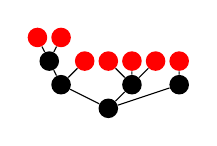
\begin{tikzpicture}[scale=.2]
\node[circle, scale=0.75, fill] (tid0) at (5.25,1.5){};
\node[circle, scale=0.75, fill] (tid1) at (2.25,3){};
\node[circle, scale=0.75, fill] (tid4) at (1.5,4.5){};
\node[circle, scale=0.75, fill, red] (tid10) at (0.75,6){};
\node[circle, scale=0.75, fill, red] (tid11) at (2.25,6){};
\draw[](tid4) -- (tid10);
\draw[](tid4) -- (tid11);
\node[circle, scale=0.75, fill, red] (tid5) at (3.75,4.5){};
\draw[](tid1) -- (tid4);
\draw[](tid1) -- (tid5);
\node[circle, scale=0.75, fill] (tid2) at (6.75,3){};
\node[circle, scale=0.75, fill, red] (tid6) at (5.25,4.5){};
\node[circle, scale=0.75, fill, red] (tid7) at (6.75,4.5){};
\node[circle, scale=0.75, fill, red] (tid8) at (8.25,4.5){};
\draw[](tid2) -- (tid6);
\draw[](tid2) -- (tid7);
\draw[](tid2) -- (tid8);
\node[circle, scale=0.75, fill] (tid3) at (9.75,3){};
\node[circle, scale=0.75, fill, red] (tid9) at (9.75,4.5){};
\draw[](tid3) -- (tid9);
\draw[](tid0) -- (tid1);
\draw[](tid0) -- (tid2);
\draw[](tid0) -- (tid3);
\end{tikzpicture}
\nodepart{three}
\footnotesize{5.38689}
\nodepart{four}
\footnotesize{$43\:14\:14\:29$}
};
 & 
\\
};
\end{scope}
\begin{scope}[yshift=\leveltopIIIII cm]
\matrix (line5)[column sep=1cm] {
\node[draw=black, rectangle split,  rectangle split parts=4] (sn0x8a1a8c0){
\footnotesize{2.17007}
\nodepart{two}
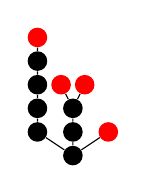
\begin{tikzpicture}[scale=.2]
\node[circle, scale=0.75, fill] (tid0) at (3,1.5){};
\node[circle, scale=0.75, fill] (tid1) at (0.75,3){};
\node[circle, scale=0.75, fill] (tid4) at (0.75,4.5){};
\node[circle, scale=0.75, fill] (tid6) at (0.75,6){};
\node[circle, scale=0.75, fill] (tid9) at (0.75,7.5){};
\node[circle, scale=0.75, fill, red] (tid10) at (0.75,9){};
\draw[](tid9) -- (tid10);
\draw[](tid6) -- (tid9);
\draw[](tid4) -- (tid6);
\draw[](tid1) -- (tid4);
\node[circle, scale=0.75, fill] (tid2) at (3,3){};
\node[circle, scale=0.75, fill] (tid5) at (3,4.5){};
\node[circle, scale=0.75, fill, red] (tid7) at (2.25,6){};
\node[circle, scale=0.75, fill, red] (tid8) at (3.75,6){};
\draw[](tid5) -- (tid7);
\draw[](tid5) -- (tid8);
\draw[](tid2) -- (tid5);
\node[circle, scale=0.75, fill, red] (tid3) at (5.25,3){};
\draw[](tid0) -- (tid1);
\draw[](tid0) -- (tid2);
\draw[](tid0) -- (tid3);
\end{tikzpicture}
\nodepart{three}
\footnotesize{6.52971}
\nodepart{four}
\footnotesize{$25\:50\:25$}
};
 & 
\node[draw=black, rectangle split,  rectangle split parts=4] (sn0x8a19970){
\footnotesize{5.71429}
\nodepart{two}
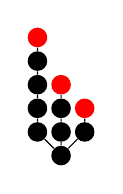
\begin{tikzpicture}[scale=.2]
\node[circle, scale=0.75, fill] (tid0) at (2.25,1.5){};
\node[circle, scale=0.75, fill] (tid1) at (0.75,3){};
\node[circle, scale=0.75, fill] (tid4) at (0.75,4.5){};
\node[circle, scale=0.75, fill] (tid7) at (0.75,6){};
\node[circle, scale=0.75, fill] (tid9) at (0.75,7.5){};
\node[circle, scale=0.75, fill, red] (tid10) at (0.75,9){};
\draw[](tid9) -- (tid10);
\draw[](tid7) -- (tid9);
\draw[](tid4) -- (tid7);
\draw[](tid1) -- (tid4);
\node[circle, scale=0.75, fill] (tid2) at (2.25,3){};
\node[circle, scale=0.75, fill] (tid5) at (2.25,4.5){};
\node[circle, scale=0.75, fill, red] (tid8) at (2.25,6){};
\draw[](tid5) -- (tid8);
\draw[](tid2) -- (tid5);
\node[circle, scale=0.75, fill] (tid3) at (3.75,3){};
\node[circle, scale=0.75, fill, red] (tid6) at (3.75,4.5){};
\draw[](tid3) -- (tid6);
\draw[](tid0) -- (tid1);
\draw[](tid0) -- (tid2);
\draw[](tid0) -- (tid3);
\end{tikzpicture}
\nodepart{three}
\footnotesize{6.46337}
\nodepart{four}
\footnotesize{$33\:33\:33$}
};
 & 
\node[draw=black, rectangle split,  rectangle split parts=4] (sn0x8a1b198){
\footnotesize{2.17007}
\nodepart{two}
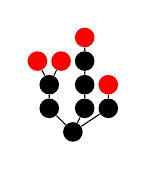
\begin{tikzpicture}[scale=.2]
\node[circle, scale=0.75, fill] (tid0) at (3,1.5){};
\node[circle, scale=0.75, fill] (tid1) at (1.5,3){};
\node[circle, scale=0.75, fill] (tid4) at (1.5,4.5){};
\node[circle, scale=0.75, fill, red] (tid7) at (0.75,6){};
\node[circle, scale=0.75, fill, red] (tid8) at (2.25,6){};
\draw[](tid4) -- (tid7);
\draw[](tid4) -- (tid8);
\draw[](tid1) -- (tid4);
\node[circle, scale=0.75, fill] (tid2) at (3.75,3){};
\node[circle, scale=0.75, fill] (tid5) at (3.75,4.5){};
\node[circle, scale=0.75, fill] (tid9) at (3.75,6){};
\node[circle, scale=0.75, fill, red] (tid10) at (3.75,7.5){};
\draw[](tid9) -- (tid10);
\draw[](tid5) -- (tid9);
\draw[](tid2) -- (tid5);
\node[circle, scale=0.75, fill] (tid3) at (5.25,3){};
\node[circle, scale=0.75, fill, red] (tid6) at (5.25,4.5){};
\draw[](tid3) -- (tid6);
\draw[](tid0) -- (tid1);
\draw[](tid0) -- (tid2);
\draw[](tid0) -- (tid3);
\end{tikzpicture}
\nodepart{three}
\footnotesize{5.93437}
\nodepart{four}
\footnotesize{$25\:50\:25$}
};
 & 
\node[draw=black, rectangle split,  rectangle split parts=4] (sn0x8a24458){
\footnotesize{0.9161}
\nodepart{two}
\begin{tikzpicture}[scale=.2]
\node[circle, scale=0.75, fill] (tid0) at (3,1.5){};
\node[circle, scale=0.75, fill] (tid1) at (2.25,3){};
\node[circle, scale=0.75, fill] (tid3) at (1.5,4.5){};
\node[circle, scale=0.75, fill, red] (tid6) at (0.75,6){};
\node[circle, scale=0.75, fill, red] (tid7) at (2.25,6){};
\draw[](tid3) -- (tid6);
\draw[](tid3) -- (tid7);
\node[circle, scale=0.75, fill, red] (tid4) at (3.75,4.5){};
\draw[](tid1) -- (tid3);
\draw[](tid1) -- (tid4);
\node[circle, scale=0.75, fill] (tid2) at (5.25,3){};
\node[circle, scale=0.75, fill] (tid5) at (5.25,4.5){};
\node[circle, scale=0.75, fill] (tid8) at (5.25,6){};
\node[circle, scale=0.75, fill] (tid9) at (5.25,7.5){};
\node[circle, scale=0.75, fill, red] (tid10) at (5.25,9){};
\draw[](tid9) -- (tid10);
\draw[](tid8) -- (tid9);
\draw[](tid5) -- (tid8);
\draw[](tid2) -- (tid5);
\draw[](tid0) -- (tid1);
\draw[](tid0) -- (tid2);
\end{tikzpicture}
\nodepart{three}
\footnotesize{6.55801}
\nodepart{four}
\footnotesize{$25\:50\:25$}
};
 & 
\node[draw=black, rectangle split,  rectangle split parts=4] (sn0x8a24b28){
\footnotesize{4.34014}
\nodepart{two}
\begin{tikzpicture}[scale=.2]
\node[circle, scale=0.75, fill] (tid0) at (3,1.5){};
\node[circle, scale=0.75, fill] (tid1) at (0.75,3){};
\node[circle, scale=0.75, fill] (tid4) at (0.75,4.5){};
\node[circle, scale=0.75, fill] (tid7) at (0.75,6){};
\node[circle, scale=0.75, fill] (tid9) at (0.75,7.5){};
\node[circle, scale=0.75, fill, red] (tid10) at (0.75,9){};
\draw[](tid9) -- (tid10);
\draw[](tid7) -- (tid9);
\draw[](tid4) -- (tid7);
\draw[](tid1) -- (tid4);
\node[circle, scale=0.75, fill] (tid2) at (3,3){};
\node[circle, scale=0.75, fill] (tid5) at (2.25,4.5){};
\node[circle, scale=0.75, fill, red] (tid8) at (2.25,6){};
\draw[](tid5) -- (tid8);
\node[circle, scale=0.75, fill, red] (tid6) at (3.75,4.5){};
\draw[](tid2) -- (tid5);
\draw[](tid2) -- (tid6);
\node[circle, scale=0.75, fill, red] (tid3) at (5.25,3){};
\draw[](tid0) -- (tid1);
\draw[](tid0) -- (tid2);
\draw[](tid0) -- (tid3);
\end{tikzpicture}
\nodepart{three}
\footnotesize{6.4402}
\nodepart{four}
\footnotesize{$25\:25\:25\:25$}
};
 & 
\node[draw=black, rectangle split,  rectangle split parts=4] (sn0x8a247f8){
\footnotesize{1.65619}
\nodepart{two}
\begin{tikzpicture}[scale=.2]
\node[circle, scale=0.75, fill] (tid0) at (3.75,1.5){};
\node[circle, scale=0.75, fill] (tid1) at (2.25,3){};
\node[circle, scale=0.75, fill] (tid4) at (1.5,4.5){};
\node[circle, scale=0.75, fill, red] (tid7) at (0.75,6){};
\node[circle, scale=0.75, fill, red] (tid8) at (2.25,6){};
\draw[](tid4) -- (tid7);
\draw[](tid4) -- (tid8);
\node[circle, scale=0.75, fill, red] (tid5) at (3.75,4.5){};
\draw[](tid1) -- (tid4);
\draw[](tid1) -- (tid5);
\node[circle, scale=0.75, fill] (tid2) at (5.25,3){};
\node[circle, scale=0.75, fill] (tid6) at (5.25,4.5){};
\node[circle, scale=0.75, fill] (tid9) at (5.25,6){};
\node[circle, scale=0.75, fill, red] (tid10) at (5.25,7.5){};
\draw[](tid9) -- (tid10);
\draw[](tid6) -- (tid9);
\draw[](tid2) -- (tid6);
\node[circle, scale=0.75, fill, red] (tid3) at (6.75,3){};
\draw[](tid0) -- (tid1);
\draw[](tid0) -- (tid2);
\draw[](tid0) -- (tid3);
\end{tikzpicture}
\nodepart{three}
\footnotesize{5.89747}
\nodepart{four}
\footnotesize{$20\:20\:40\:20$}
};
 & 
\node[draw=black, rectangle split,  rectangle split parts=4] (sn0x8a2b710){
\footnotesize{2.50794}
\nodepart{two}
\begin{tikzpicture}[scale=.2]
\node[circle, scale=0.75, fill] (tid0) at (3,1.5){};
\node[circle, scale=0.75, fill] (tid1) at (0.75,3){};
\node[circle, scale=0.75, fill] (tid4) at (0.75,4.5){};
\node[circle, scale=0.75, fill] (tid8) at (0.75,6){};
\node[circle, scale=0.75, fill] (tid9) at (0.75,7.5){};
\node[circle, scale=0.75, fill, red] (tid10) at (0.75,9){};
\draw[](tid9) -- (tid10);
\draw[](tid8) -- (tid9);
\draw[](tid4) -- (tid8);
\draw[](tid1) -- (tid4);
\node[circle, scale=0.75, fill] (tid2) at (3,3){};
\node[circle, scale=0.75, fill, red] (tid5) at (2.25,4.5){};
\node[circle, scale=0.75, fill, red] (tid6) at (3.75,4.5){};
\draw[](tid2) -- (tid5);
\draw[](tid2) -- (tid6);
\node[circle, scale=0.75, fill] (tid3) at (5.25,3){};
\node[circle, scale=0.75, fill, red] (tid7) at (5.25,4.5){};
\draw[](tid3) -- (tid7);
\draw[](tid0) -- (tid1);
\draw[](tid0) -- (tid2);
\draw[](tid0) -- (tid3);
\end{tikzpicture}
\nodepart{three}
\footnotesize{6.32904}
\nodepart{four}
\footnotesize{$50\:25\:25$}
};
 & 
\node[draw=black, rectangle split,  rectangle split parts=4] (sn0x8a29208){
\footnotesize{4.34014}
\nodepart{two}
\begin{tikzpicture}[scale=.2]
\node[circle, scale=0.75, fill] (tid0) at (3,1.5){};
\node[circle, scale=0.75, fill] (tid1) at (1.5,3){};
\node[circle, scale=0.75, fill] (tid4) at (0.75,4.5){};
\node[circle, scale=0.75, fill, red] (tid8) at (0.75,6){};
\draw[](tid4) -- (tid8);
\node[circle, scale=0.75, fill, red] (tid5) at (2.25,4.5){};
\draw[](tid1) -- (tid4);
\draw[](tid1) -- (tid5);
\node[circle, scale=0.75, fill] (tid2) at (3.75,3){};
\node[circle, scale=0.75, fill] (tid6) at (3.75,4.5){};
\node[circle, scale=0.75, fill] (tid9) at (3.75,6){};
\node[circle, scale=0.75, fill, red] (tid10) at (3.75,7.5){};
\draw[](tid9) -- (tid10);
\draw[](tid6) -- (tid9);
\draw[](tid2) -- (tid6);
\node[circle, scale=0.75, fill] (tid3) at (5.25,3){};
\node[circle, scale=0.75, fill, red] (tid7) at (5.25,4.5){};
\draw[](tid3) -- (tid7);
\draw[](tid0) -- (tid1);
\draw[](tid0) -- (tid2);
\draw[](tid0) -- (tid3);
\end{tikzpicture}
\nodepart{three}
\footnotesize{5.81909}
\nodepart{four}
\footnotesize{$25\:25\:25\:25$}
};
 & 
\node[draw=black, rectangle split,  rectangle split parts=4] (sn0x8a2d7f0){
\footnotesize{0.828096}
\nodepart{two}
\begin{tikzpicture}[scale=.2]
\node[circle, scale=0.75, fill] (tid0) at (3.75,1.5){};
\node[circle, scale=0.75, fill] (tid1) at (2.25,3){};
\node[circle, scale=0.75, fill] (tid4) at (1.5,4.5){};
\node[circle, scale=0.75, fill, red] (tid8) at (0.75,6){};
\node[circle, scale=0.75, fill, red] (tid9) at (2.25,6){};
\draw[](tid4) -- (tid8);
\draw[](tid4) -- (tid9);
\node[circle, scale=0.75, fill, red] (tid5) at (3.75,4.5){};
\draw[](tid1) -- (tid4);
\draw[](tid1) -- (tid5);
\node[circle, scale=0.75, fill] (tid2) at (5.25,3){};
\node[circle, scale=0.75, fill] (tid6) at (5.25,4.5){};
\node[circle, scale=0.75, fill, red] (tid10) at (5.25,6){};
\draw[](tid6) -- (tid10);
\draw[](tid2) -- (tid6);
\node[circle, scale=0.75, fill] (tid3) at (6.75,3){};
\node[circle, scale=0.75, fill, red] (tid7) at (6.75,4.5){};
\draw[](tid3) -- (tid7);
\draw[](tid0) -- (tid1);
\draw[](tid0) -- (tid2);
\draw[](tid0) -- (tid3);
\end{tikzpicture}
\nodepart{three}
\footnotesize{5.49543}
\nodepart{four}
\footnotesize{$20\:20\:40\:20$}
};
 & 
\node[draw=black, rectangle split,  rectangle split parts=4] (sn0x8a2dd70){
\footnotesize{1.8322}
\nodepart{two}
\begin{tikzpicture}[scale=.2]
\node[circle, scale=0.75, fill] (tid0) at (3,1.5){};
\node[circle, scale=0.75, fill] (tid1) at (1.5,3){};
\node[circle, scale=0.75, fill] (tid3) at (0.75,4.5){};
\node[circle, scale=0.75, fill] (tid6) at (0.75,6){};
\node[circle, scale=0.75, fill] (tid9) at (0.75,7.5){};
\node[circle, scale=0.75, fill, red] (tid10) at (0.75,9){};
\draw[](tid9) -- (tid10);
\draw[](tid6) -- (tid9);
\draw[](tid3) -- (tid6);
\node[circle, scale=0.75, fill, red] (tid4) at (2.25,4.5){};
\draw[](tid1) -- (tid3);
\draw[](tid1) -- (tid4);
\node[circle, scale=0.75, fill] (tid2) at (4.5,3){};
\node[circle, scale=0.75, fill] (tid5) at (4.5,4.5){};
\node[circle, scale=0.75, fill, red] (tid7) at (3.75,6){};
\node[circle, scale=0.75, fill, red] (tid8) at (5.25,6){};
\draw[](tid5) -- (tid7);
\draw[](tid5) -- (tid8);
\draw[](tid2) -- (tid5);
\draw[](tid0) -- (tid1);
\draw[](tid0) -- (tid2);
\end{tikzpicture}
\nodepart{three}
\footnotesize{6.55061}
\nodepart{four}
\footnotesize{$25\:50\:25$}
};
 & 
\node[draw=black, rectangle split,  rectangle split parts=4] (sn0x8a2ef70){
\footnotesize{8.68027}
\nodepart{two}
\begin{tikzpicture}[scale=.2]
\node[circle, scale=0.75, fill] (tid0) at (3,1.5){};
\node[circle, scale=0.75, fill] (tid1) at (1.5,3){};
\node[circle, scale=0.75, fill] (tid4) at (0.75,4.5){};
\node[circle, scale=0.75, fill] (tid7) at (0.75,6){};
\node[circle, scale=0.75, fill] (tid9) at (0.75,7.5){};
\node[circle, scale=0.75, fill, red] (tid10) at (0.75,9){};
\draw[](tid9) -- (tid10);
\draw[](tid7) -- (tid9);
\draw[](tid4) -- (tid7);
\node[circle, scale=0.75, fill, red] (tid5) at (2.25,4.5){};
\draw[](tid1) -- (tid4);
\draw[](tid1) -- (tid5);
\node[circle, scale=0.75, fill] (tid2) at (3.75,3){};
\node[circle, scale=0.75, fill] (tid6) at (3.75,4.5){};
\node[circle, scale=0.75, fill, red] (tid8) at (3.75,6){};
\draw[](tid6) -- (tid8);
\draw[](tid2) -- (tid6);
\node[circle, scale=0.75, fill, red] (tid3) at (5.25,3){};
\draw[](tid0) -- (tid1);
\draw[](tid0) -- (tid2);
\draw[](tid0) -- (tid3);
\end{tikzpicture}
\nodepart{three}
\footnotesize{6.42739}
\nodepart{four}
\footnotesize{$25\:25\:25\:25$}
};
 & 
\node[draw=black, rectangle split,  rectangle split parts=4] (sn0x8a2dfd8){
\footnotesize{3.31239}
\nodepart{two}
\begin{tikzpicture}[scale=.2]
\node[circle, scale=0.75, fill] (tid0) at (3.75,1.5){};
\node[circle, scale=0.75, fill] (tid1) at (1.5,3){};
\node[circle, scale=0.75, fill] (tid4) at (0.75,4.5){};
\node[circle, scale=0.75, fill] (tid7) at (0.75,6){};
\node[circle, scale=0.75, fill, red] (tid10) at (0.75,7.5){};
\draw[](tid7) -- (tid10);
\draw[](tid4) -- (tid7);
\node[circle, scale=0.75, fill, red] (tid5) at (2.25,4.5){};
\draw[](tid1) -- (tid4);
\draw[](tid1) -- (tid5);
\node[circle, scale=0.75, fill] (tid2) at (4.5,3){};
\node[circle, scale=0.75, fill] (tid6) at (4.5,4.5){};
\node[circle, scale=0.75, fill, red] (tid8) at (3.75,6){};
\node[circle, scale=0.75, fill, red] (tid9) at (5.25,6){};
\draw[](tid6) -- (tid8);
\draw[](tid6) -- (tid9);
\draw[](tid2) -- (tid6);
\node[circle, scale=0.75, fill, red] (tid3) at (6.75,3){};
\draw[](tid0) -- (tid1);
\draw[](tid0) -- (tid2);
\draw[](tid0) -- (tid3);
\end{tikzpicture}
\nodepart{three}
\footnotesize{5.89412}
\nodepart{four}
\footnotesize{$20\:20\:40\:20$}
};
 & 
\node[draw=black, rectangle split,  rectangle split parts=4] (sn0x8a339f8){
\footnotesize{6.4127}
\nodepart{two}
\begin{tikzpicture}[scale=.2]
\node[circle, scale=0.75, fill] (tid0) at (3,1.5){};
\node[circle, scale=0.75, fill] (tid1) at (1.5,3){};
\node[circle, scale=0.75, fill] (tid4) at (0.75,4.5){};
\node[circle, scale=0.75, fill] (tid8) at (0.75,6){};
\node[circle, scale=0.75, fill] (tid9) at (0.75,7.5){};
\node[circle, scale=0.75, fill, red] (tid10) at (0.75,9){};
\draw[](tid9) -- (tid10);
\draw[](tid8) -- (tid9);
\draw[](tid4) -- (tid8);
\node[circle, scale=0.75, fill, red] (tid5) at (2.25,4.5){};
\draw[](tid1) -- (tid4);
\draw[](tid1) -- (tid5);
\node[circle, scale=0.75, fill] (tid2) at (3.75,3){};
\node[circle, scale=0.75, fill, red] (tid6) at (3.75,4.5){};
\draw[](tid2) -- (tid6);
\node[circle, scale=0.75, fill] (tid3) at (5.25,3){};
\node[circle, scale=0.75, fill, red] (tid7) at (5.25,4.5){};
\draw[](tid3) -- (tid7);
\draw[](tid0) -- (tid1);
\draw[](tid0) -- (tid2);
\draw[](tid0) -- (tid3);
\end{tikzpicture}
\nodepart{three}
\footnotesize{6.30417}
\nodepart{four}
\footnotesize{$25\:50\:25$}
};
 & 
\node[draw=black, rectangle split,  rectangle split parts=4] (sn0x8a33a60){
\footnotesize{8.68027}
\nodepart{two}
\begin{tikzpicture}[scale=.2]
\node[circle, scale=0.75, fill] (tid0) at (3,1.5){};
\node[circle, scale=0.75, fill] (tid1) at (1.5,3){};
\node[circle, scale=0.75, fill] (tid4) at (0.75,4.5){};
\node[circle, scale=0.75, fill] (tid8) at (0.75,6){};
\node[circle, scale=0.75, fill, red] (tid10) at (0.75,7.5){};
\draw[](tid8) -- (tid10);
\draw[](tid4) -- (tid8);
\node[circle, scale=0.75, fill, red] (tid5) at (2.25,4.5){};
\draw[](tid1) -- (tid4);
\draw[](tid1) -- (tid5);
\node[circle, scale=0.75, fill] (tid2) at (3.75,3){};
\node[circle, scale=0.75, fill] (tid6) at (3.75,4.5){};
\node[circle, scale=0.75, fill, red] (tid9) at (3.75,6){};
\draw[](tid6) -- (tid9);
\draw[](tid2) -- (tid6);
\node[circle, scale=0.75, fill] (tid3) at (5.25,3){};
\node[circle, scale=0.75, fill, red] (tid7) at (5.25,4.5){};
\draw[](tid3) -- (tid7);
\draw[](tid0) -- (tid1);
\draw[](tid0) -- (tid2);
\draw[](tid0) -- (tid3);
\end{tikzpicture}
\nodepart{three}
\footnotesize{5.8091}
\nodepart{four}
\footnotesize{$25\:25\:25\:25$}
};
 & 
\node[draw=black, rectangle split,  rectangle split parts=4] (sn0x8a34318){
\footnotesize{1.65619}
\nodepart{two}
\begin{tikzpicture}[scale=.2]
\node[circle, scale=0.75, fill] (tid0) at (3.75,1.5){};
\node[circle, scale=0.75, fill] (tid1) at (1.5,3){};
\node[circle, scale=0.75, fill] (tid4) at (0.75,4.5){};
\node[circle, scale=0.75, fill, red] (tid8) at (0.75,6){};
\draw[](tid4) -- (tid8);
\node[circle, scale=0.75, fill, red] (tid5) at (2.25,4.5){};
\draw[](tid1) -- (tid4);
\draw[](tid1) -- (tid5);
\node[circle, scale=0.75, fill] (tid2) at (4.5,3){};
\node[circle, scale=0.75, fill] (tid6) at (4.5,4.5){};
\node[circle, scale=0.75, fill, red] (tid9) at (3.75,6){};
\node[circle, scale=0.75, fill, red] (tid10) at (5.25,6){};
\draw[](tid6) -- (tid9);
\draw[](tid6) -- (tid10);
\draw[](tid2) -- (tid6);
\node[circle, scale=0.75, fill] (tid3) at (6.75,3){};
\node[circle, scale=0.75, fill, red] (tid7) at (6.75,4.5){};
\draw[](tid3) -- (tid7);
\draw[](tid0) -- (tid1);
\draw[](tid0) -- (tid2);
\draw[](tid0) -- (tid3);
\end{tikzpicture}
\nodepart{three}
\footnotesize{5.50314}
\nodepart{four}
\footnotesize{$20\:40\:20\:20$}
};
 & 
\node[draw=black, rectangle split,  rectangle split parts=4] (sn0x8a35560){
\footnotesize{3.6644}
\nodepart{two}
\begin{tikzpicture}[scale=.2]
\node[circle, scale=0.75, fill] (tid0) at (3,1.5){};
\node[circle, scale=0.75, fill] (tid1) at (1.5,3){};
\node[circle, scale=0.75, fill] (tid3) at (0.75,4.5){};
\node[circle, scale=0.75, fill] (tid7) at (0.75,6){};
\node[circle, scale=0.75, fill] (tid9) at (0.75,7.5){};
\node[circle, scale=0.75, fill, red] (tid10) at (0.75,9){};
\draw[](tid9) -- (tid10);
\draw[](tid7) -- (tid9);
\draw[](tid3) -- (tid7);
\node[circle, scale=0.75, fill, red] (tid4) at (2.25,4.5){};
\draw[](tid1) -- (tid3);
\draw[](tid1) -- (tid4);
\node[circle, scale=0.75, fill] (tid2) at (4.5,3){};
\node[circle, scale=0.75, fill] (tid5) at (3.75,4.5){};
\node[circle, scale=0.75, fill, red] (tid8) at (3.75,6){};
\draw[](tid5) -- (tid8);
\node[circle, scale=0.75, fill, red] (tid6) at (5.25,4.5){};
\draw[](tid2) -- (tid5);
\draw[](tid2) -- (tid6);
\draw[](tid0) -- (tid1);
\draw[](tid0) -- (tid2);
\end{tikzpicture}
\nodepart{three}
\footnotesize{6.46237}
\nodepart{four}
\footnotesize{$25\:25\:25\:25$}
};
 & 
\node[draw=black, rectangle split,  rectangle split parts=4] (sn0x8a366b8){
\footnotesize{1.42425}
\nodepart{two}
\begin{tikzpicture}[scale=.2]
\node[circle, scale=0.75, fill] (tid0) at (3.75,1.5){};
\node[circle, scale=0.75, fill] (tid1) at (2.25,3){};
\node[circle, scale=0.75, fill] (tid3) at (1.5,4.5){};
\node[circle, scale=0.75, fill, red] (tid7) at (0.75,6){};
\node[circle, scale=0.75, fill, red] (tid8) at (2.25,6){};
\draw[](tid3) -- (tid7);
\draw[](tid3) -- (tid8);
\node[circle, scale=0.75, fill, red] (tid4) at (3.75,4.5){};
\draw[](tid1) -- (tid3);
\draw[](tid1) -- (tid4);
\node[circle, scale=0.75, fill] (tid2) at (6,3){};
\node[circle, scale=0.75, fill] (tid5) at (5.25,4.5){};
\node[circle, scale=0.75, fill] (tid9) at (5.25,6){};
\node[circle, scale=0.75, fill, red] (tid10) at (5.25,7.5){};
\draw[](tid9) -- (tid10);
\draw[](tid5) -- (tid9);
\node[circle, scale=0.75, fill, red] (tid6) at (6.75,4.5){};
\draw[](tid2) -- (tid5);
\draw[](tid2) -- (tid6);
\draw[](tid0) -- (tid1);
\draw[](tid0) -- (tid2);
\end{tikzpicture}
\nodepart{three}
\footnotesize{5.93266}
\nodepart{four}
\footnotesize{$20\:20\:40\:20$}
};
 & 
\node[draw=black, rectangle split,  rectangle split parts=4] (sn0x8a389e0){
\footnotesize{3.77627}
\nodepart{two}
\begin{tikzpicture}[scale=.2]
\node[circle, scale=0.75, fill] (tid0) at (3.75,1.5){};
\node[circle, scale=0.75, fill] (tid1) at (1.5,3){};
\node[circle, scale=0.75, fill] (tid4) at (0.75,4.5){};
\node[circle, scale=0.75, fill] (tid8) at (0.75,6){};
\node[circle, scale=0.75, fill] (tid9) at (0.75,7.5){};
\node[circle, scale=0.75, fill, red] (tid10) at (0.75,9){};
\draw[](tid9) -- (tid10);
\draw[](tid8) -- (tid9);
\draw[](tid4) -- (tid8);
\node[circle, scale=0.75, fill, red] (tid5) at (2.25,4.5){};
\draw[](tid1) -- (tid4);
\draw[](tid1) -- (tid5);
\node[circle, scale=0.75, fill] (tid2) at (4.5,3){};
\node[circle, scale=0.75, fill, red] (tid6) at (3.75,4.5){};
\node[circle, scale=0.75, fill, red] (tid7) at (5.25,4.5){};
\draw[](tid2) -- (tid6);
\draw[](tid2) -- (tid7);
\node[circle, scale=0.75, fill, red] (tid3) at (6.75,3){};
\draw[](tid0) -- (tid1);
\draw[](tid0) -- (tid2);
\draw[](tid0) -- (tid3);
\end{tikzpicture}
\nodepart{three}
\footnotesize{6.28894}
\nodepart{four}
\footnotesize{$20\:40\:20\:20$}
};
 & 
\node[draw=black, rectangle split,  rectangle split parts=4] (sn0x8a38c68){
\footnotesize{6.62477}
\nodepart{two}
\begin{tikzpicture}[scale=.2]
\node[circle, scale=0.75, fill] (tid0) at (3.75,1.5){};
\node[circle, scale=0.75, fill] (tid1) at (1.5,3){};
\node[circle, scale=0.75, fill] (tid4) at (0.75,4.5){};
\node[circle, scale=0.75, fill] (tid8) at (0.75,6){};
\node[circle, scale=0.75, fill, red] (tid10) at (0.75,7.5){};
\draw[](tid8) -- (tid10);
\draw[](tid4) -- (tid8);
\node[circle, scale=0.75, fill, red] (tid5) at (2.25,4.5){};
\draw[](tid1) -- (tid4);
\draw[](tid1) -- (tid5);
\node[circle, scale=0.75, fill] (tid2) at (4.5,3){};
\node[circle, scale=0.75, fill] (tid6) at (3.75,4.5){};
\node[circle, scale=0.75, fill, red] (tid9) at (3.75,6){};
\draw[](tid6) -- (tid9);
\node[circle, scale=0.75, fill, red] (tid7) at (5.25,4.5){};
\draw[](tid2) -- (tid6);
\draw[](tid2) -- (tid7);
\node[circle, scale=0.75, fill, red] (tid3) at (6.75,3){};
\draw[](tid0) -- (tid1);
\draw[](tid0) -- (tid2);
\draw[](tid0) -- (tid3);
\end{tikzpicture}
\nodepart{three}
\footnotesize{5.77558}
\nodepart{four}
\footnotesize{$20\:20\:20\:20\:20$}
};
 & 
\node[draw=black, rectangle split,  rectangle split parts=4] (sn0x8a39dc8){
\footnotesize{1.2784}
\nodepart{two}
\begin{tikzpicture}[scale=.2]
\node[circle, scale=0.75, fill] (tid0) at (4.5,1.5){};
\node[circle, scale=0.75, fill] (tid1) at (2.25,3){};
\node[circle, scale=0.75, fill] (tid4) at (1.5,4.5){};
\node[circle, scale=0.75, fill, red] (tid8) at (0.75,6){};
\node[circle, scale=0.75, fill, red] (tid9) at (2.25,6){};
\draw[](tid4) -- (tid8);
\draw[](tid4) -- (tid9);
\node[circle, scale=0.75, fill, red] (tid5) at (3.75,4.5){};
\draw[](tid1) -- (tid4);
\draw[](tid1) -- (tid5);
\node[circle, scale=0.75, fill] (tid2) at (6,3){};
\node[circle, scale=0.75, fill] (tid6) at (5.25,4.5){};
\node[circle, scale=0.75, fill, red] (tid10) at (5.25,6){};
\draw[](tid6) -- (tid10);
\node[circle, scale=0.75, fill, red] (tid7) at (6.75,4.5){};
\draw[](tid2) -- (tid6);
\draw[](tid2) -- (tid7);
\node[circle, scale=0.75, fill, red] (tid3) at (8.25,3){};
\draw[](tid0) -- (tid1);
\draw[](tid0) -- (tid2);
\draw[](tid0) -- (tid3);
\end{tikzpicture}
\nodepart{three}
\footnotesize{5.45544}
\nodepart{four}
\footnotesize{$17\:17\:17\:33\:17$}
};
 & 
\node[draw=black, rectangle split,  rectangle split parts=4] (sn0x8a3b9b8){
\footnotesize{3.77627}
\nodepart{two}
\begin{tikzpicture}[scale=.2]
\node[circle, scale=0.75, fill] (tid0) at (3.75,1.5){};
\node[circle, scale=0.75, fill] (tid1) at (1.5,3){};
\node[circle, scale=0.75, fill] (tid4) at (0.75,4.5){};
\node[circle, scale=0.75, fill] (tid9) at (0.75,6){};
\node[circle, scale=0.75, fill, red] (tid10) at (0.75,7.5){};
\draw[](tid9) -- (tid10);
\draw[](tid4) -- (tid9);
\node[circle, scale=0.75, fill, red] (tid5) at (2.25,4.5){};
\draw[](tid1) -- (tid4);
\draw[](tid1) -- (tid5);
\node[circle, scale=0.75, fill] (tid2) at (4.5,3){};
\node[circle, scale=0.75, fill, red] (tid6) at (3.75,4.5){};
\node[circle, scale=0.75, fill, red] (tid7) at (5.25,4.5){};
\draw[](tid2) -- (tid6);
\draw[](tid2) -- (tid7);
\node[circle, scale=0.75, fill] (tid3) at (6.75,3){};
\node[circle, scale=0.75, fill, red] (tid8) at (6.75,4.5){};
\draw[](tid3) -- (tid8);
\draw[](tid0) -- (tid1);
\draw[](tid0) -- (tid2);
\draw[](tid0) -- (tid3);
\end{tikzpicture}
\nodepart{three}
\footnotesize{5.62824}
\nodepart{four}
\footnotesize{$20\:40\:20\:20$}
};
 & 
\node[draw=black, rectangle split,  rectangle split parts=4] (sn0x8a3b840){
\footnotesize{3.31239}
\nodepart{two}
\begin{tikzpicture}[scale=.2]
\node[circle, scale=0.75, fill] (tid0) at (3.75,1.5){};
\node[circle, scale=0.75, fill] (tid1) at (1.5,3){};
\node[circle, scale=0.75, fill] (tid4) at (0.75,4.5){};
\node[circle, scale=0.75, fill, red] (tid9) at (0.75,6){};
\draw[](tid4) -- (tid9);
\node[circle, scale=0.75, fill, red] (tid5) at (2.25,4.5){};
\draw[](tid1) -- (tid4);
\draw[](tid1) -- (tid5);
\node[circle, scale=0.75, fill] (tid2) at (4.5,3){};
\node[circle, scale=0.75, fill] (tid6) at (3.75,4.5){};
\node[circle, scale=0.75, fill, red] (tid10) at (3.75,6){};
\draw[](tid6) -- (tid10);
\node[circle, scale=0.75, fill, red] (tid7) at (5.25,4.5){};
\draw[](tid2) -- (tid6);
\draw[](tid2) -- (tid7);
\node[circle, scale=0.75, fill] (tid3) at (6.75,3){};
\node[circle, scale=0.75, fill, red] (tid8) at (6.75,4.5){};
\draw[](tid3) -- (tid8);
\draw[](tid0) -- (tid1);
\draw[](tid0) -- (tid2);
\draw[](tid0) -- (tid3);
\end{tikzpicture}
\nodepart{three}
\footnotesize{5.36302}
\nodepart{four}
\footnotesize{$40\:20\:40$}
};
 & 
\node[draw=black, rectangle split,  rectangle split parts=4] (sn0x8a3cc00){
\footnotesize{0.467784}
\nodepart{two}
\begin{tikzpicture}[scale=.2]
\node[circle, scale=0.75, fill] (tid0) at (4.5,1.5){};
\node[circle, scale=0.75, fill] (tid1) at (2.25,3){};
\node[circle, scale=0.75, fill] (tid4) at (1.5,4.5){};
\node[circle, scale=0.75, fill, red] (tid9) at (0.75,6){};
\node[circle, scale=0.75, fill, red] (tid10) at (2.25,6){};
\draw[](tid4) -- (tid9);
\draw[](tid4) -- (tid10);
\node[circle, scale=0.75, fill, red] (tid5) at (3.75,4.5){};
\draw[](tid1) -- (tid4);
\draw[](tid1) -- (tid5);
\node[circle, scale=0.75, fill] (tid2) at (6,3){};
\node[circle, scale=0.75, fill, red] (tid6) at (5.25,4.5){};
\node[circle, scale=0.75, fill, red] (tid7) at (6.75,4.5){};
\draw[](tid2) -- (tid6);
\draw[](tid2) -- (tid7);
\node[circle, scale=0.75, fill] (tid3) at (8.25,3){};
\node[circle, scale=0.75, fill, red] (tid8) at (8.25,4.5){};
\draw[](tid3) -- (tid8);
\draw[](tid0) -- (tid1);
\draw[](tid0) -- (tid2);
\draw[](tid0) -- (tid3);
\end{tikzpicture}
\nodepart{three}
\footnotesize{5.28707}
\nodepart{four}
\footnotesize{$33\:17\:17\:33$}
};
 & 
\node[draw=black, rectangle split,  rectangle split parts=4] (sn0x8a3f168){
\footnotesize{1.8322}
\nodepart{two}
\begin{tikzpicture}[scale=.2]
\node[circle, scale=0.75, fill] (tid0) at (3,1.5){};
\node[circle, scale=0.75, fill] (tid1) at (2.25,3){};
\node[circle, scale=0.75, fill] (tid3) at (0.75,4.5){};
\node[circle, scale=0.75, fill] (tid7) at (0.75,6){};
\node[circle, scale=0.75, fill] (tid9) at (0.75,7.5){};
\node[circle, scale=0.75, fill, red] (tid10) at (0.75,9){};
\draw[](tid9) -- (tid10);
\draw[](tid7) -- (tid9);
\draw[](tid3) -- (tid7);
\node[circle, scale=0.75, fill, red] (tid4) at (2.25,4.5){};
\node[circle, scale=0.75, fill, red] (tid5) at (3.75,4.5){};
\draw[](tid1) -- (tid3);
\draw[](tid1) -- (tid4);
\draw[](tid1) -- (tid5);
\node[circle, scale=0.75, fill] (tid2) at (5.25,3){};
\node[circle, scale=0.75, fill] (tid6) at (5.25,4.5){};
\node[circle, scale=0.75, fill, red] (tid8) at (5.25,6){};
\draw[](tid6) -- (tid8);
\draw[](tid2) -- (tid6);
\draw[](tid0) -- (tid1);
\draw[](tid0) -- (tid2);
\end{tikzpicture}
\nodepart{three}
\footnotesize{6.44886}
\nodepart{four}
\footnotesize{$50\:25\:25$}
};
 & 
\node[draw=black, rectangle split,  rectangle split parts=4] (sn0x8a3ed30){
\footnotesize{0.712126}
\nodepart{two}
\begin{tikzpicture}[scale=.2]
\node[circle, scale=0.75, fill] (tid0) at (3.75,1.5){};
\node[circle, scale=0.75, fill] (tid1) at (2.25,3){};
\node[circle, scale=0.75, fill] (tid3) at (0.75,4.5){};
\node[circle, scale=0.75, fill] (tid7) at (0.75,6){};
\node[circle, scale=0.75, fill, red] (tid10) at (0.75,7.5){};
\draw[](tid7) -- (tid10);
\draw[](tid3) -- (tid7);
\node[circle, scale=0.75, fill, red] (tid4) at (2.25,4.5){};
\node[circle, scale=0.75, fill, red] (tid5) at (3.75,4.5){};
\draw[](tid1) -- (tid3);
\draw[](tid1) -- (tid4);
\draw[](tid1) -- (tid5);
\node[circle, scale=0.75, fill] (tid2) at (6,3){};
\node[circle, scale=0.75, fill] (tid6) at (6,4.5){};
\node[circle, scale=0.75, fill, red] (tid8) at (5.25,6){};
\node[circle, scale=0.75, fill, red] (tid9) at (6.75,6){};
\draw[](tid6) -- (tid8);
\draw[](tid6) -- (tid9);
\draw[](tid2) -- (tid6);
\draw[](tid0) -- (tid1);
\draw[](tid0) -- (tid2);
\end{tikzpicture}
\nodepart{three}
\footnotesize{5.92724}
\nodepart{four}
\footnotesize{$40\:40\:20$}
};
 & 
\node[draw=black, rectangle split,  rectangle split parts=4] (sn0x8a42ff0){
\footnotesize{3.12321}
\nodepart{two}
\begin{tikzpicture}[scale=.2]
\node[circle, scale=0.75, fill] (tid0) at (3.75,1.5){};
\node[circle, scale=0.75, fill] (tid1) at (2.25,3){};
\node[circle, scale=0.75, fill] (tid4) at (0.75,4.5){};
\node[circle, scale=0.75, fill] (tid8) at (0.75,6){};
\node[circle, scale=0.75, fill] (tid9) at (0.75,7.5){};
\node[circle, scale=0.75, fill, red] (tid10) at (0.75,9){};
\draw[](tid9) -- (tid10);
\draw[](tid8) -- (tid9);
\draw[](tid4) -- (tid8);
\node[circle, scale=0.75, fill, red] (tid5) at (2.25,4.5){};
\node[circle, scale=0.75, fill, red] (tid6) at (3.75,4.5){};
\draw[](tid1) -- (tid4);
\draw[](tid1) -- (tid5);
\draw[](tid1) -- (tid6);
\node[circle, scale=0.75, fill] (tid2) at (5.25,3){};
\node[circle, scale=0.75, fill, red] (tid7) at (5.25,4.5){};
\draw[](tid2) -- (tid7);
\node[circle, scale=0.75, fill, red] (tid3) at (6.75,3){};
\draw[](tid0) -- (tid1);
\draw[](tid0) -- (tid2);
\draw[](tid0) -- (tid3);
\end{tikzpicture}
\nodepart{three}
\footnotesize{6.26193}
\nodepart{four}
\footnotesize{$40\:20\:20\:20$}
};
 & 
\node[draw=black, rectangle split,  rectangle split parts=4] (sn0x8a431a8){
\footnotesize{3.31239}
\nodepart{two}
\begin{tikzpicture}[scale=.2]
\node[circle, scale=0.75, fill] (tid0) at (3.75,1.5){};
\node[circle, scale=0.75, fill] (tid1) at (2.25,3){};
\node[circle, scale=0.75, fill] (tid4) at (0.75,4.5){};
\node[circle, scale=0.75, fill] (tid8) at (0.75,6){};
\node[circle, scale=0.75, fill, red] (tid10) at (0.75,7.5){};
\draw[](tid8) -- (tid10);
\draw[](tid4) -- (tid8);
\node[circle, scale=0.75, fill, red] (tid5) at (2.25,4.5){};
\node[circle, scale=0.75, fill, red] (tid6) at (3.75,4.5){};
\draw[](tid1) -- (tid4);
\draw[](tid1) -- (tid5);
\draw[](tid1) -- (tid6);
\node[circle, scale=0.75, fill] (tid2) at (5.25,3){};
\node[circle, scale=0.75, fill] (tid7) at (5.25,4.5){};
\node[circle, scale=0.75, fill, red] (tid9) at (5.25,6){};
\draw[](tid7) -- (tid9);
\draw[](tid2) -- (tid7);
\node[circle, scale=0.75, fill, red] (tid3) at (6.75,3){};
\draw[](tid0) -- (tid1);
\draw[](tid0) -- (tid2);
\draw[](tid0) -- (tid3);
\end{tikzpicture}
\nodepart{three}
\footnotesize{5.76277}
\nodepart{four}
\footnotesize{$40\:20\:20\:20$}
};
 & 
\node[draw=black, rectangle split,  rectangle split parts=4] (sn0x8a45dd0){
\footnotesize{0.639201}
\nodepart{two}
\begin{tikzpicture}[scale=.2]
\node[circle, scale=0.75, fill] (tid0) at (4.5,1.5){};
\node[circle, scale=0.75, fill] (tid1) at (2.25,3){};
\node[circle, scale=0.75, fill] (tid4) at (0.75,4.5){};
\node[circle, scale=0.75, fill, red] (tid8) at (0.75,6){};
\draw[](tid4) -- (tid8);
\node[circle, scale=0.75, fill, red] (tid5) at (2.25,4.5){};
\node[circle, scale=0.75, fill, red] (tid6) at (3.75,4.5){};
\draw[](tid1) -- (tid4);
\draw[](tid1) -- (tid5);
\draw[](tid1) -- (tid6);
\node[circle, scale=0.75, fill] (tid2) at (6,3){};
\node[circle, scale=0.75, fill] (tid7) at (6,4.5){};
\node[circle, scale=0.75, fill, red] (tid9) at (5.25,6){};
\node[circle, scale=0.75, fill, red] (tid10) at (6.75,6){};
\draw[](tid7) -- (tid9);
\draw[](tid7) -- (tid10);
\draw[](tid2) -- (tid7);
\node[circle, scale=0.75, fill, red] (tid3) at (8.25,3){};
\draw[](tid0) -- (tid1);
\draw[](tid0) -- (tid2);
\draw[](tid0) -- (tid3);
\end{tikzpicture}
\nodepart{three}
\footnotesize{5.45806}
\nodepart{four}
\footnotesize{$33\:17\:33\:17$}
};
 & 
\node[draw=black, rectangle split,  rectangle split parts=4] (sn0x8a45c68){
\footnotesize{2.42479}
\nodepart{two}
\begin{tikzpicture}[scale=.2]
\node[circle, scale=0.75, fill] (tid0) at (3.75,1.5){};
\node[circle, scale=0.75, fill] (tid1) at (2.25,3){};
\node[circle, scale=0.75, fill] (tid4) at (0.75,4.5){};
\node[circle, scale=0.75, fill] (tid9) at (0.75,6){};
\node[circle, scale=0.75, fill, red] (tid10) at (0.75,7.5){};
\draw[](tid9) -- (tid10);
\draw[](tid4) -- (tid9);
\node[circle, scale=0.75, fill, red] (tid5) at (2.25,4.5){};
\node[circle, scale=0.75, fill, red] (tid6) at (3.75,4.5){};
\draw[](tid1) -- (tid4);
\draw[](tid1) -- (tid5);
\draw[](tid1) -- (tid6);
\node[circle, scale=0.75, fill] (tid2) at (5.25,3){};
\node[circle, scale=0.75, fill, red] (tid7) at (5.25,4.5){};
\draw[](tid2) -- (tid7);
\node[circle, scale=0.75, fill] (tid3) at (6.75,3){};
\node[circle, scale=0.75, fill, red] (tid8) at (6.75,4.5){};
\draw[](tid3) -- (tid8);
\draw[](tid0) -- (tid1);
\draw[](tid0) -- (tid2);
\draw[](tid0) -- (tid3);
\end{tikzpicture}
\nodepart{three}
\footnotesize{5.59831}
\nodepart{four}
\footnotesize{$40\:40\:20$}
};
 & 
\node[draw=black, rectangle split,  rectangle split parts=4] (sn0x8a462e0){
\footnotesize{1.65619}
\nodepart{two}
\begin{tikzpicture}[scale=.2]
\node[circle, scale=0.75, fill] (tid0) at (3.75,1.5){};
\node[circle, scale=0.75, fill] (tid1) at (2.25,3){};
\node[circle, scale=0.75, fill] (tid4) at (0.75,4.5){};
\node[circle, scale=0.75, fill, red] (tid9) at (0.75,6){};
\draw[](tid4) -- (tid9);
\node[circle, scale=0.75, fill, red] (tid5) at (2.25,4.5){};
\node[circle, scale=0.75, fill, red] (tid6) at (3.75,4.5){};
\draw[](tid1) -- (tid4);
\draw[](tid1) -- (tid5);
\draw[](tid1) -- (tid6);
\node[circle, scale=0.75, fill] (tid2) at (5.25,3){};
\node[circle, scale=0.75, fill] (tid7) at (5.25,4.5){};
\node[circle, scale=0.75, fill, red] (tid10) at (5.25,6){};
\draw[](tid7) -- (tid10);
\draw[](tid2) -- (tid7);
\node[circle, scale=0.75, fill] (tid3) at (6.75,3){};
\node[circle, scale=0.75, fill, red] (tid8) at (6.75,4.5){};
\draw[](tid3) -- (tid8);
\draw[](tid0) -- (tid1);
\draw[](tid0) -- (tid2);
\draw[](tid0) -- (tid3);
\end{tikzpicture}
\nodepart{three}
\footnotesize{5.35739}
\nodepart{four}
\footnotesize{$40\:20\:20\:20$}
};
 & 
\node[draw=black, rectangle split,  rectangle split parts=4] (sn0x8a468e0){
\footnotesize{0.213067}
\nodepart{two}
\begin{tikzpicture}[scale=.2]
\node[circle, scale=0.75, fill] (tid0) at (4.5,1.5){};
\node[circle, scale=0.75, fill] (tid1) at (2.25,3){};
\node[circle, scale=0.75, fill, red] (tid4) at (0.75,4.5){};
\node[circle, scale=0.75, fill, red] (tid5) at (2.25,4.5){};
\node[circle, scale=0.75, fill, red] (tid6) at (3.75,4.5){};
\draw[](tid1) -- (tid4);
\draw[](tid1) -- (tid5);
\draw[](tid1) -- (tid6);
\node[circle, scale=0.75, fill] (tid2) at (6,3){};
\node[circle, scale=0.75, fill] (tid7) at (6,4.5){};
\node[circle, scale=0.75, fill, red] (tid9) at (5.25,6){};
\node[circle, scale=0.75, fill, red] (tid10) at (6.75,6){};
\draw[](tid7) -- (tid9);
\draw[](tid7) -- (tid10);
\draw[](tid2) -- (tid7);
\node[circle, scale=0.75, fill] (tid3) at (8.25,3){};
\node[circle, scale=0.75, fill, red] (tid8) at (8.25,4.5){};
\draw[](tid3) -- (tid8);
\draw[](tid0) -- (tid1);
\draw[](tid0) -- (tid2);
\draw[](tid0) -- (tid3);
\end{tikzpicture}
\nodepart{three}
\footnotesize{5.30249}
\nodepart{four}
\footnotesize{$50\:17\:33$}
};
 & 
\node[draw=black, rectangle split,  rectangle split parts=4] (sn0x8a49928){
\footnotesize{0.808768}
\nodepart{two}
\begin{tikzpicture}[scale=.2]
\node[circle, scale=0.75, fill] (tid0) at (3.75,1.5){};
\node[circle, scale=0.75, fill] (tid1) at (2.25,3){};
\node[circle, scale=0.75, fill] (tid3) at (0.75,4.5){};
\node[circle, scale=0.75, fill] (tid8) at (0.75,6){};
\node[circle, scale=0.75, fill] (tid9) at (0.75,7.5){};
\node[circle, scale=0.75, fill, red] (tid10) at (0.75,9){};
\draw[](tid9) -- (tid10);
\draw[](tid8) -- (tid9);
\draw[](tid3) -- (tid8);
\node[circle, scale=0.75, fill, red] (tid4) at (2.25,4.5){};
\node[circle, scale=0.75, fill, red] (tid5) at (3.75,4.5){};
\draw[](tid1) -- (tid3);
\draw[](tid1) -- (tid4);
\draw[](tid1) -- (tid5);
\node[circle, scale=0.75, fill] (tid2) at (6,3){};
\node[circle, scale=0.75, fill, red] (tid6) at (5.25,4.5){};
\node[circle, scale=0.75, fill, red] (tid7) at (6.75,4.5){};
\draw[](tid2) -- (tid6);
\draw[](tid2) -- (tid7);
\draw[](tid0) -- (tid1);
\draw[](tid0) -- (tid2);
\end{tikzpicture}
\nodepart{three}
\footnotesize{6.31248}
\nodepart{four}
\footnotesize{$40\:40\:20$}
};
 & 
\node[draw=black, rectangle split,  rectangle split parts=4] (sn0x8a4a5a0){
\footnotesize{1.42425}
\nodepart{two}
\begin{tikzpicture}[scale=.2]
\node[circle, scale=0.75, fill] (tid0) at (3.75,1.5){};
\node[circle, scale=0.75, fill] (tid1) at (2.25,3){};
\node[circle, scale=0.75, fill] (tid3) at (0.75,4.5){};
\node[circle, scale=0.75, fill] (tid8) at (0.75,6){};
\node[circle, scale=0.75, fill, red] (tid10) at (0.75,7.5){};
\draw[](tid8) -- (tid10);
\draw[](tid3) -- (tid8);
\node[circle, scale=0.75, fill, red] (tid4) at (2.25,4.5){};
\node[circle, scale=0.75, fill, red] (tid5) at (3.75,4.5){};
\draw[](tid1) -- (tid3);
\draw[](tid1) -- (tid4);
\draw[](tid1) -- (tid5);
\node[circle, scale=0.75, fill] (tid2) at (6,3){};
\node[circle, scale=0.75, fill] (tid6) at (5.25,4.5){};
\node[circle, scale=0.75, fill, red] (tid9) at (5.25,6){};
\draw[](tid6) -- (tid9);
\node[circle, scale=0.75, fill, red] (tid7) at (6.75,4.5){};
\draw[](tid2) -- (tid6);
\draw[](tid2) -- (tid7);
\draw[](tid0) -- (tid1);
\draw[](tid0) -- (tid2);
\end{tikzpicture}
\nodepart{three}
\footnotesize{5.81097}
\nodepart{four}
\footnotesize{$40\:20\:20\:20$}
};
 & 
\node[draw=black, rectangle split,  rectangle split parts=4] (sn0x8a4bff8){
\footnotesize{0.278819}
\nodepart{two}
\begin{tikzpicture}[scale=.2]
\node[circle, scale=0.75, fill] (tid0) at (4.5,1.5){};
\node[circle, scale=0.75, fill] (tid1) at (2.25,3){};
\node[circle, scale=0.75, fill] (tid3) at (0.75,4.5){};
\node[circle, scale=0.75, fill, red] (tid8) at (0.75,6){};
\draw[](tid3) -- (tid8);
\node[circle, scale=0.75, fill, red] (tid4) at (2.25,4.5){};
\node[circle, scale=0.75, fill, red] (tid5) at (3.75,4.5){};
\draw[](tid1) -- (tid3);
\draw[](tid1) -- (tid4);
\draw[](tid1) -- (tid5);
\node[circle, scale=0.75, fill] (tid2) at (6.75,3){};
\node[circle, scale=0.75, fill] (tid6) at (6,4.5){};
\node[circle, scale=0.75, fill, red] (tid9) at (5.25,6){};
\node[circle, scale=0.75, fill, red] (tid10) at (6.75,6){};
\draw[](tid6) -- (tid9);
\draw[](tid6) -- (tid10);
\node[circle, scale=0.75, fill, red] (tid7) at (8.25,4.5){};
\draw[](tid2) -- (tid6);
\draw[](tid2) -- (tid7);
\draw[](tid0) -- (tid1);
\draw[](tid0) -- (tid2);
\end{tikzpicture}
\nodepart{three}
\footnotesize{5.50591}
\nodepart{four}
\footnotesize{$33\:17\:33\:17$}
};
 & 
\node[draw=black, rectangle split,  rectangle split parts=4] (sn0x8a4c5d8){
\footnotesize{1.44153}
\nodepart{two}
\begin{tikzpicture}[scale=.2]
\node[circle, scale=0.75, fill] (tid0) at (4.5,1.5){};
\node[circle, scale=0.75, fill] (tid1) at (2.25,3){};
\node[circle, scale=0.75, fill] (tid4) at (0.75,4.5){};
\node[circle, scale=0.75, fill] (tid9) at (0.75,6){};
\node[circle, scale=0.75, fill, red] (tid10) at (0.75,7.5){};
\draw[](tid9) -- (tid10);
\draw[](tid4) -- (tid9);
\node[circle, scale=0.75, fill, red] (tid5) at (2.25,4.5){};
\node[circle, scale=0.75, fill, red] (tid6) at (3.75,4.5){};
\draw[](tid1) -- (tid4);
\draw[](tid1) -- (tid5);
\draw[](tid1) -- (tid6);
\node[circle, scale=0.75, fill] (tid2) at (6,3){};
\node[circle, scale=0.75, fill, red] (tid7) at (5.25,4.5){};
\node[circle, scale=0.75, fill, red] (tid8) at (6.75,4.5){};
\draw[](tid2) -- (tid7);
\draw[](tid2) -- (tid8);
\node[circle, scale=0.75, fill, red] (tid3) at (8.25,3){};
\draw[](tid0) -- (tid1);
\draw[](tid0) -- (tid2);
\draw[](tid0) -- (tid3);
\end{tikzpicture}
\nodepart{three}
\footnotesize{5.5757}
\nodepart{four}
\footnotesize{$33\:33\:17\:17$}
};
 & 
\node[draw=black, rectangle split,  rectangle split parts=4] (sn0x8a4ec68){
\footnotesize{1.2784}
\nodepart{two}
\begin{tikzpicture}[scale=.2]
\node[circle, scale=0.75, fill] (tid0) at (4.5,1.5){};
\node[circle, scale=0.75, fill] (tid1) at (2.25,3){};
\node[circle, scale=0.75, fill] (tid4) at (0.75,4.5){};
\node[circle, scale=0.75, fill, red] (tid9) at (0.75,6){};
\draw[](tid4) -- (tid9);
\node[circle, scale=0.75, fill, red] (tid5) at (2.25,4.5){};
\node[circle, scale=0.75, fill, red] (tid6) at (3.75,4.5){};
\draw[](tid1) -- (tid4);
\draw[](tid1) -- (tid5);
\draw[](tid1) -- (tid6);
\node[circle, scale=0.75, fill] (tid2) at (6,3){};
\node[circle, scale=0.75, fill] (tid7) at (5.25,4.5){};
\node[circle, scale=0.75, fill, red] (tid10) at (5.25,6){};
\draw[](tid7) -- (tid10);
\node[circle, scale=0.75, fill, red] (tid8) at (6.75,4.5){};
\draw[](tid2) -- (tid7);
\draw[](tid2) -- (tid8);
\node[circle, scale=0.75, fill, red] (tid3) at (8.25,3){};
\draw[](tid0) -- (tid1);
\draw[](tid0) -- (tid2);
\draw[](tid0) -- (tid3);
\end{tikzpicture}
\nodepart{three}
\footnotesize{5.31381}
\nodepart{four}
\footnotesize{$33\:17\:17\:17\:17$}
};
 & 
\node[draw=black, rectangle split,  rectangle split parts=4] (sn0x8a4f758){
\footnotesize{0.166597}
\nodepart{two}
\begin{tikzpicture}[scale=.2]
\node[circle, scale=0.75, fill] (tid0) at (5.25,1.5){};
\node[circle, scale=0.75, fill] (tid1) at (2.25,3){};
\node[circle, scale=0.75, fill] (tid4) at (1.5,4.5){};
\node[circle, scale=0.75, fill, red] (tid9) at (0.75,6){};
\node[circle, scale=0.75, fill, red] (tid10) at (2.25,6){};
\draw[](tid4) -- (tid9);
\draw[](tid4) -- (tid10);
\node[circle, scale=0.75, fill, red] (tid5) at (3.75,4.5){};
\draw[](tid1) -- (tid4);
\draw[](tid1) -- (tid5);
\node[circle, scale=0.75, fill] (tid2) at (6.75,3){};
\node[circle, scale=0.75, fill, red] (tid6) at (5.25,4.5){};
\node[circle, scale=0.75, fill, red] (tid7) at (6.75,4.5){};
\node[circle, scale=0.75, fill, red] (tid8) at (8.25,4.5){};
\draw[](tid2) -- (tid6);
\draw[](tid2) -- (tid7);
\draw[](tid2) -- (tid8);
\node[circle, scale=0.75, fill, red] (tid3) at (9.75,3){};
\draw[](tid0) -- (tid1);
\draw[](tid0) -- (tid2);
\draw[](tid0) -- (tid3);
\end{tikzpicture}
\nodepart{three}
\footnotesize{5.24816}
\nodepart{four}
\footnotesize{$43\:14\:14\:29$}
};
 & 
\node[draw=black, rectangle split,  rectangle split parts=4] (sn0x8a50c58){
\footnotesize{0.720765}
\nodepart{two}
\begin{tikzpicture}[scale=.2]
\node[circle, scale=0.75, fill] (tid0) at (4.5,1.5){};
\node[circle, scale=0.75, fill] (tid1) at (2.25,3){};
\node[circle, scale=0.75, fill] (tid4) at (0.75,4.5){};
\node[circle, scale=0.75, fill, red] (tid10) at (0.75,6){};
\draw[](tid4) -- (tid10);
\node[circle, scale=0.75, fill, red] (tid5) at (2.25,4.5){};
\node[circle, scale=0.75, fill, red] (tid6) at (3.75,4.5){};
\draw[](tid1) -- (tid4);
\draw[](tid1) -- (tid5);
\draw[](tid1) -- (tid6);
\node[circle, scale=0.75, fill] (tid2) at (6,3){};
\node[circle, scale=0.75, fill, red] (tid7) at (5.25,4.5){};
\node[circle, scale=0.75, fill, red] (tid8) at (6.75,4.5){};
\draw[](tid2) -- (tid7);
\draw[](tid2) -- (tid8);
\node[circle, scale=0.75, fill] (tid3) at (8.25,3){};
\node[circle, scale=0.75, fill, red] (tid9) at (8.25,4.5){};
\draw[](tid3) -- (tid9);
\draw[](tid0) -- (tid1);
\draw[](tid0) -- (tid2);
\draw[](tid0) -- (tid3);
\end{tikzpicture}
\nodepart{three}
\footnotesize{5.13451}
\nodepart{four}
\footnotesize{$33\:33\:17\:17$}
};
 & 
\node[draw=black, rectangle split,  rectangle split parts=4] (sn0x8a50878){
\footnotesize{0.426134}
\nodepart{two}
\begin{tikzpicture}[scale=.2]
\node[circle, scale=0.75, fill] (tid0) at (4.5,1.5){};
\node[circle, scale=0.75, fill] (tid1) at (2.25,3){};
\node[circle, scale=0.75, fill, red] (tid4) at (0.75,4.5){};
\node[circle, scale=0.75, fill, red] (tid5) at (2.25,4.5){};
\node[circle, scale=0.75, fill, red] (tid6) at (3.75,4.5){};
\draw[](tid1) -- (tid4);
\draw[](tid1) -- (tid5);
\draw[](tid1) -- (tid6);
\node[circle, scale=0.75, fill] (tid2) at (6,3){};
\node[circle, scale=0.75, fill] (tid7) at (5.25,4.5){};
\node[circle, scale=0.75, fill, red] (tid10) at (5.25,6){};
\draw[](tid7) -- (tid10);
\node[circle, scale=0.75, fill, red] (tid8) at (6.75,4.5){};
\draw[](tid2) -- (tid7);
\draw[](tid2) -- (tid8);
\node[circle, scale=0.75, fill] (tid3) at (8.25,3){};
\node[circle, scale=0.75, fill, red] (tid9) at (8.25,4.5){};
\draw[](tid3) -- (tid9);
\draw[](tid0) -- (tid1);
\draw[](tid0) -- (tid2);
\draw[](tid0) -- (tid3);
\end{tikzpicture}
\nodepart{three}
\footnotesize{5.14819}
\nodepart{four}
\footnotesize{$50\:17\:17\:17$}
};
 & 
\\
};
\end{scope}
\begin{scope}[yshift=\leveltopIIIIII cm]
\matrix (line6)[column sep=1cm] {
\node[draw=black, rectangle split,  rectangle split parts=4] (sn0x8a1b678){
\footnotesize{1.22959}
\nodepart{two}
\begin{tikzpicture}[scale=.2]
\node[circle, scale=0.75, fill] (tid0) at (2.25,1.5){};
\node[circle, scale=0.75, fill] (tid1) at (0.75,3){};
\node[circle, scale=0.75, fill] (tid3) at (0.75,4.5){};
\node[circle, scale=0.75, fill] (tid5) at (0.75,6){};
\node[circle, scale=0.75, fill] (tid8) at (0.75,7.5){};
\node[circle, scale=0.75, fill, red] (tid9) at (0.75,9){};
\draw[](tid8) -- (tid9);
\draw[](tid5) -- (tid8);
\draw[](tid3) -- (tid5);
\draw[](tid1) -- (tid3);
\node[circle, scale=0.75, fill] (tid2) at (3,3){};
\node[circle, scale=0.75, fill] (tid4) at (3,4.5){};
\node[circle, scale=0.75, fill, red] (tid6) at (2.25,6){};
\node[circle, scale=0.75, fill, red] (tid7) at (3.75,6){};
\draw[](tid4) -- (tid6);
\draw[](tid4) -- (tid7);
\draw[](tid2) -- (tid4);
\draw[](tid0) -- (tid1);
\draw[](tid0) -- (tid2);
\end{tikzpicture}
\nodepart{three}
\footnotesize{6.51357}
\nodepart{four}
\footnotesize{$67\:33$}
};
 & 
\node[draw=black, rectangle split,  rectangle split parts=4] (sn0x8a19860){
\footnotesize{6.2449}
\nodepart{two}
\begin{tikzpicture}[scale=.2]
\node[circle, scale=0.75, fill] (tid0) at (2.25,1.5){};
\node[circle, scale=0.75, fill] (tid1) at (0.75,3){};
\node[circle, scale=0.75, fill] (tid4) at (0.75,4.5){};
\node[circle, scale=0.75, fill] (tid6) at (0.75,6){};
\node[circle, scale=0.75, fill] (tid8) at (0.75,7.5){};
\node[circle, scale=0.75, fill, red] (tid9) at (0.75,9){};
\draw[](tid8) -- (tid9);
\draw[](tid6) -- (tid8);
\draw[](tid4) -- (tid6);
\draw[](tid1) -- (tid4);
\node[circle, scale=0.75, fill] (tid2) at (2.25,3){};
\node[circle, scale=0.75, fill] (tid5) at (2.25,4.5){};
\node[circle, scale=0.75, fill, red] (tid7) at (2.25,6){};
\draw[](tid5) -- (tid7);
\draw[](tid2) -- (tid5);
\node[circle, scale=0.75, fill, red] (tid3) at (3.75,3){};
\draw[](tid0) -- (tid1);
\draw[](tid0) -- (tid2);
\draw[](tid0) -- (tid3);
\end{tikzpicture}
\nodepart{three}
\footnotesize{6.38626}
\nodepart{four}
\footnotesize{$33\:33\:33$}
};
 & 
\node[draw=black, rectangle split,  rectangle split parts=4] (sn0x8a1b968){
\footnotesize{2.07875}
\nodepart{two}
\begin{tikzpicture}[scale=.2]
\node[circle, scale=0.75, fill] (tid0) at (3,1.5){};
\node[circle, scale=0.75, fill] (tid1) at (1.5,3){};
\node[circle, scale=0.75, fill] (tid4) at (1.5,4.5){};
\node[circle, scale=0.75, fill, red] (tid6) at (0.75,6){};
\node[circle, scale=0.75, fill, red] (tid7) at (2.25,6){};
\draw[](tid4) -- (tid6);
\draw[](tid4) -- (tid7);
\draw[](tid1) -- (tid4);
\node[circle, scale=0.75, fill] (tid2) at (3.75,3){};
\node[circle, scale=0.75, fill] (tid5) at (3.75,4.5){};
\node[circle, scale=0.75, fill] (tid8) at (3.75,6){};
\node[circle, scale=0.75, fill, red] (tid9) at (3.75,7.5){};
\draw[](tid8) -- (tid9);
\draw[](tid5) -- (tid8);
\draw[](tid2) -- (tid5);
\node[circle, scale=0.75, fill, red] (tid3) at (5.25,3){};
\draw[](tid0) -- (tid1);
\draw[](tid0) -- (tid2);
\draw[](tid0) -- (tid3);
\end{tikzpicture}
\nodepart{three}
\footnotesize{5.83275}
\nodepart{four}
\footnotesize{$25\:50\:25$}
};
 & 
\node[draw=black, rectangle split,  rectangle split parts=4] (sn0x8a1f5f0){
\footnotesize{4.76191}
\nodepart{two}
\begin{tikzpicture}[scale=.2]
\node[circle, scale=0.75, fill] (tid0) at (2.25,1.5){};
\node[circle, scale=0.75, fill] (tid1) at (0.75,3){};
\node[circle, scale=0.75, fill] (tid4) at (0.75,4.5){};
\node[circle, scale=0.75, fill] (tid7) at (0.75,6){};
\node[circle, scale=0.75, fill] (tid8) at (0.75,7.5){};
\node[circle, scale=0.75, fill, red] (tid9) at (0.75,9){};
\draw[](tid8) -- (tid9);
\draw[](tid7) -- (tid8);
\draw[](tid4) -- (tid7);
\draw[](tid1) -- (tid4);
\node[circle, scale=0.75, fill] (tid2) at (2.25,3){};
\node[circle, scale=0.75, fill, red] (tid5) at (2.25,4.5){};
\draw[](tid2) -- (tid5);
\node[circle, scale=0.75, fill] (tid3) at (3.75,3){};
\node[circle, scale=0.75, fill, red] (tid6) at (3.75,4.5){};
\draw[](tid3) -- (tid6);
\draw[](tid0) -- (tid1);
\draw[](tid0) -- (tid2);
\draw[](tid0) -- (tid3);
\end{tikzpicture}
\nodepart{three}
\footnotesize{6.25896}
\nodepart{four}
\footnotesize{$67\:33$}
};
 & 
\node[draw=black, rectangle split,  rectangle split parts=4] (sn0x8a22640){
\footnotesize{6.2449}
\nodepart{two}
\begin{tikzpicture}[scale=.2]
\node[circle, scale=0.75, fill] (tid0) at (2.25,1.5){};
\node[circle, scale=0.75, fill] (tid1) at (0.75,3){};
\node[circle, scale=0.75, fill] (tid4) at (0.75,4.5){};
\node[circle, scale=0.75, fill] (tid7) at (0.75,6){};
\node[circle, scale=0.75, fill, red] (tid9) at (0.75,7.5){};
\draw[](tid7) -- (tid9);
\draw[](tid4) -- (tid7);
\draw[](tid1) -- (tid4);
\node[circle, scale=0.75, fill] (tid2) at (2.25,3){};
\node[circle, scale=0.75, fill] (tid5) at (2.25,4.5){};
\node[circle, scale=0.75, fill, red] (tid8) at (2.25,6){};
\draw[](tid5) -- (tid8);
\draw[](tid2) -- (tid5);
\node[circle, scale=0.75, fill] (tid3) at (3.75,3){};
\node[circle, scale=0.75, fill, red] (tid6) at (3.75,4.5){};
\draw[](tid3) -- (tid6);
\draw[](tid0) -- (tid1);
\draw[](tid0) -- (tid2);
\draw[](tid0) -- (tid3);
\end{tikzpicture}
\nodepart{three}
\footnotesize{5.7449}
\nodepart{four}
\footnotesize{$33\:33\:33$}
};
 & 
\node[draw=black, rectangle split,  rectangle split parts=4] (sn0x8a23d10){
\footnotesize{1.03937}
\nodepart{two}
\begin{tikzpicture}[scale=.2]
\node[circle, scale=0.75, fill] (tid0) at (3,1.5){};
\node[circle, scale=0.75, fill] (tid1) at (1.5,3){};
\node[circle, scale=0.75, fill] (tid4) at (1.5,4.5){};
\node[circle, scale=0.75, fill, red] (tid7) at (0.75,6){};
\node[circle, scale=0.75, fill, red] (tid8) at (2.25,6){};
\draw[](tid4) -- (tid7);
\draw[](tid4) -- (tid8);
\draw[](tid1) -- (tid4);
\node[circle, scale=0.75, fill] (tid2) at (3.75,3){};
\node[circle, scale=0.75, fill] (tid5) at (3.75,4.5){};
\node[circle, scale=0.75, fill, red] (tid9) at (3.75,6){};
\draw[](tid5) -- (tid9);
\draw[](tid2) -- (tid5);
\node[circle, scale=0.75, fill] (tid3) at (5.25,3){};
\node[circle, scale=0.75, fill, red] (tid6) at (5.25,4.5){};
\draw[](tid3) -- (tid6);
\draw[](tid0) -- (tid1);
\draw[](tid0) -- (tid2);
\draw[](tid0) -- (tid3);
\end{tikzpicture}
\nodepart{three}
\footnotesize{5.41491}
\nodepart{four}
\footnotesize{$25\:50\:25$}
};
 & 
\node[draw=black, rectangle split,  rectangle split parts=4] (sn0x8a23bf0){
\footnotesize{2.45918}
\nodepart{two}
\begin{tikzpicture}[scale=.2]
\node[circle, scale=0.75, fill] (tid0) at (2.25,1.5){};
\node[circle, scale=0.75, fill] (tid1) at (0.75,3){};
\node[circle, scale=0.75, fill] (tid3) at (0.75,4.5){};
\node[circle, scale=0.75, fill] (tid6) at (0.75,6){};
\node[circle, scale=0.75, fill] (tid8) at (0.75,7.5){};
\node[circle, scale=0.75, fill, red] (tid9) at (0.75,9){};
\draw[](tid8) -- (tid9);
\draw[](tid6) -- (tid8);
\draw[](tid3) -- (tid6);
\draw[](tid1) -- (tid3);
\node[circle, scale=0.75, fill] (tid2) at (3,3){};
\node[circle, scale=0.75, fill] (tid4) at (2.25,4.5){};
\node[circle, scale=0.75, fill, red] (tid7) at (2.25,6){};
\draw[](tid4) -- (tid7);
\node[circle, scale=0.75, fill, red] (tid5) at (3.75,4.5){};
\draw[](tid2) -- (tid4);
\draw[](tid2) -- (tid5);
\draw[](tid0) -- (tid1);
\draw[](tid0) -- (tid2);
\end{tikzpicture}
\nodepart{three}
\footnotesize{6.42264}
\nodepart{four}
\footnotesize{$33\:33\:33$}
};
 & 
\node[draw=black, rectangle split,  rectangle split parts=4] (sn0x8a25a00){
\footnotesize{0.845114}
\nodepart{two}
\begin{tikzpicture}[scale=.2]
\node[circle, scale=0.75, fill] (tid0) at (3,1.5){};
\node[circle, scale=0.75, fill] (tid1) at (2.25,3){};
\node[circle, scale=0.75, fill] (tid3) at (1.5,4.5){};
\node[circle, scale=0.75, fill, red] (tid6) at (0.75,6){};
\node[circle, scale=0.75, fill, red] (tid7) at (2.25,6){};
\draw[](tid3) -- (tid6);
\draw[](tid3) -- (tid7);
\node[circle, scale=0.75, fill, red] (tid4) at (3.75,4.5){};
\draw[](tid1) -- (tid3);
\draw[](tid1) -- (tid4);
\node[circle, scale=0.75, fill] (tid2) at (5.25,3){};
\node[circle, scale=0.75, fill] (tid5) at (5.25,4.5){};
\node[circle, scale=0.75, fill] (tid8) at (5.25,6){};
\node[circle, scale=0.75, fill, red] (tid9) at (5.25,7.5){};
\draw[](tid8) -- (tid9);
\draw[](tid5) -- (tid8);
\draw[](tid2) -- (tid5);
\draw[](tid0) -- (tid1);
\draw[](tid0) -- (tid2);
\end{tikzpicture}
\nodepart{three}
\footnotesize{5.87321}
\nodepart{four}
\footnotesize{$25\:50\:25$}
};
 & 
\node[draw=black, rectangle split,  rectangle split parts=4] (sn0x8a28110){
\footnotesize{2.46727}
\nodepart{two}
\begin{tikzpicture}[scale=.2]
\node[circle, scale=0.75, fill] (tid0) at (3,1.5){};
\node[circle, scale=0.75, fill] (tid1) at (0.75,3){};
\node[circle, scale=0.75, fill] (tid4) at (0.75,4.5){};
\node[circle, scale=0.75, fill] (tid7) at (0.75,6){};
\node[circle, scale=0.75, fill] (tid8) at (0.75,7.5){};
\node[circle, scale=0.75, fill, red] (tid9) at (0.75,9){};
\draw[](tid8) -- (tid9);
\draw[](tid7) -- (tid8);
\draw[](tid4) -- (tid7);
\draw[](tid1) -- (tid4);
\node[circle, scale=0.75, fill] (tid2) at (3,3){};
\node[circle, scale=0.75, fill, red] (tid5) at (2.25,4.5){};
\node[circle, scale=0.75, fill, red] (tid6) at (3.75,4.5){};
\draw[](tid2) -- (tid5);
\draw[](tid2) -- (tid6);
\node[circle, scale=0.75, fill, red] (tid3) at (5.25,3){};
\draw[](tid0) -- (tid1);
\draw[](tid0) -- (tid2);
\draw[](tid0) -- (tid3);
\end{tikzpicture}
\nodepart{three}
\footnotesize{6.24282}
\nodepart{four}
\footnotesize{$50\:25\:25$}
};
 & 
\node[draw=black, rectangle split,  rectangle split parts=4] (sn0x8a28c28){
\footnotesize{4.1575}
\nodepart{two}
\begin{tikzpicture}[scale=.2]
\node[circle, scale=0.75, fill] (tid0) at (3,1.5){};
\node[circle, scale=0.75, fill] (tid1) at (1.5,3){};
\node[circle, scale=0.75, fill] (tid4) at (0.75,4.5){};
\node[circle, scale=0.75, fill, red] (tid7) at (0.75,6){};
\draw[](tid4) -- (tid7);
\node[circle, scale=0.75, fill, red] (tid5) at (2.25,4.5){};
\draw[](tid1) -- (tid4);
\draw[](tid1) -- (tid5);
\node[circle, scale=0.75, fill] (tid2) at (3.75,3){};
\node[circle, scale=0.75, fill] (tid6) at (3.75,4.5){};
\node[circle, scale=0.75, fill] (tid8) at (3.75,6){};
\node[circle, scale=0.75, fill, red] (tid9) at (3.75,7.5){};
\draw[](tid8) -- (tid9);
\draw[](tid6) -- (tid8);
\draw[](tid2) -- (tid6);
\node[circle, scale=0.75, fill, red] (tid3) at (5.25,3){};
\draw[](tid0) -- (tid1);
\draw[](tid0) -- (tid2);
\draw[](tid0) -- (tid3);
\end{tikzpicture}
\nodepart{three}
\footnotesize{5.70909}
\nodepart{four}
\footnotesize{$25\:25\:25\:25$}
};
 & 
\node[draw=black, rectangle split,  rectangle split parts=4] (sn0x8a2aea8){
\footnotesize{0.709925}
\nodepart{two}
\begin{tikzpicture}[scale=.2]
\node[circle, scale=0.75, fill] (tid0) at (3.75,1.5){};
\node[circle, scale=0.75, fill] (tid1) at (2.25,3){};
\node[circle, scale=0.75, fill] (tid4) at (1.5,4.5){};
\node[circle, scale=0.75, fill, red] (tid7) at (0.75,6){};
\node[circle, scale=0.75, fill, red] (tid8) at (2.25,6){};
\draw[](tid4) -- (tid7);
\draw[](tid4) -- (tid8);
\node[circle, scale=0.75, fill, red] (tid5) at (3.75,4.5){};
\draw[](tid1) -- (tid4);
\draw[](tid1) -- (tid5);
\node[circle, scale=0.75, fill] (tid2) at (5.25,3){};
\node[circle, scale=0.75, fill] (tid6) at (5.25,4.5){};
\node[circle, scale=0.75, fill, red] (tid9) at (5.25,6){};
\draw[](tid6) -- (tid9);
\draw[](tid2) -- (tid6);
\node[circle, scale=0.75, fill, red] (tid3) at (6.75,3){};
\draw[](tid0) -- (tid1);
\draw[](tid0) -- (tid2);
\draw[](tid0) -- (tid3);
\end{tikzpicture}
\nodepart{three}
\footnotesize{5.3632}
\nodepart{four}
\footnotesize{$20\:20\:40\:20$}
};
 & 
\node[draw=black, rectangle split,  rectangle split parts=4] (sn0x8a2ba60){
\footnotesize{2.46727}
\nodepart{two}
\begin{tikzpicture}[scale=.2]
\node[circle, scale=0.75, fill] (tid0) at (3,1.5){};
\node[circle, scale=0.75, fill] (tid1) at (0.75,3){};
\node[circle, scale=0.75, fill] (tid4) at (0.75,4.5){};
\node[circle, scale=0.75, fill] (tid8) at (0.75,6){};
\node[circle, scale=0.75, fill, red] (tid9) at (0.75,7.5){};
\draw[](tid8) -- (tid9);
\draw[](tid4) -- (tid8);
\draw[](tid1) -- (tid4);
\node[circle, scale=0.75, fill] (tid2) at (3,3){};
\node[circle, scale=0.75, fill, red] (tid5) at (2.25,4.5){};
\node[circle, scale=0.75, fill, red] (tid6) at (3.75,4.5){};
\draw[](tid2) -- (tid5);
\draw[](tid2) -- (tid6);
\node[circle, scale=0.75, fill] (tid3) at (5.25,3){};
\node[circle, scale=0.75, fill, red] (tid7) at (5.25,4.5){};
\draw[](tid3) -- (tid7);
\draw[](tid0) -- (tid1);
\draw[](tid0) -- (tid2);
\draw[](tid0) -- (tid3);
\end{tikzpicture}
\nodepart{three}
\footnotesize{5.55543}
\nodepart{four}
\footnotesize{$50\:25\:25$}
};
 & 
\node[draw=black, rectangle split,  rectangle split parts=4] (sn0x8a2c1f8){
\footnotesize{6.23625}
\nodepart{two}
\begin{tikzpicture}[scale=.2]
\node[circle, scale=0.75, fill] (tid0) at (3,1.5){};
\node[circle, scale=0.75, fill] (tid1) at (1.5,3){};
\node[circle, scale=0.75, fill] (tid4) at (0.75,4.5){};
\node[circle, scale=0.75, fill, red] (tid8) at (0.75,6){};
\draw[](tid4) -- (tid8);
\node[circle, scale=0.75, fill, red] (tid5) at (2.25,4.5){};
\draw[](tid1) -- (tid4);
\draw[](tid1) -- (tid5);
\node[circle, scale=0.75, fill] (tid2) at (3.75,3){};
\node[circle, scale=0.75, fill] (tid6) at (3.75,4.5){};
\node[circle, scale=0.75, fill, red] (tid9) at (3.75,6){};
\draw[](tid6) -- (tid9);
\draw[](tid2) -- (tid6);
\node[circle, scale=0.75, fill] (tid3) at (5.25,3){};
\node[circle, scale=0.75, fill, red] (tid7) at (5.25,4.5){};
\draw[](tid3) -- (tid7);
\draw[](tid0) -- (tid1);
\draw[](tid0) -- (tid2);
\draw[](tid0) -- (tid3);
\end{tikzpicture}
\nodepart{three}
\footnotesize{5.26694}
\nodepart{four}
\footnotesize{$25\:25\:25\:25$}
};
 & 
\node[draw=black, rectangle split,  rectangle split parts=4] (sn0x8a2cc20){
\footnotesize{0.321547}
\nodepart{two}
\begin{tikzpicture}[scale=.2]
\node[circle, scale=0.75, fill] (tid0) at (3.75,1.5){};
\node[circle, scale=0.75, fill] (tid1) at (2.25,3){};
\node[circle, scale=0.75, fill] (tid4) at (1.5,4.5){};
\node[circle, scale=0.75, fill, red] (tid8) at (0.75,6){};
\node[circle, scale=0.75, fill, red] (tid9) at (2.25,6){};
\draw[](tid4) -- (tid8);
\draw[](tid4) -- (tid9);
\node[circle, scale=0.75, fill, red] (tid5) at (3.75,4.5){};
\draw[](tid1) -- (tid4);
\draw[](tid1) -- (tid5);
\node[circle, scale=0.75, fill] (tid2) at (5.25,3){};
\node[circle, scale=0.75, fill, red] (tid6) at (5.25,4.5){};
\draw[](tid2) -- (tid6);
\node[circle, scale=0.75, fill] (tid3) at (6.75,3){};
\node[circle, scale=0.75, fill, red] (tid7) at (6.75,4.5){};
\draw[](tid3) -- (tid7);
\draw[](tid0) -- (tid1);
\draw[](tid0) -- (tid2);
\draw[](tid0) -- (tid3);
\end{tikzpicture}
\nodepart{three}
\footnotesize{5.16517}
\nodepart{four}
\footnotesize{$20\:40\:40$}
};
 & 
\node[draw=black, rectangle split,  rectangle split parts=4] (sn0x8a2fd00){
\footnotesize{4.91837}
\nodepart{two}
\begin{tikzpicture}[scale=.2]
\node[circle, scale=0.75, fill] (tid0) at (2.25,1.5){};
\node[circle, scale=0.75, fill] (tid1) at (1.5,3){};
\node[circle, scale=0.75, fill] (tid3) at (0.75,4.5){};
\node[circle, scale=0.75, fill] (tid6) at (0.75,6){};
\node[circle, scale=0.75, fill] (tid8) at (0.75,7.5){};
\node[circle, scale=0.75, fill, red] (tid9) at (0.75,9){};
\draw[](tid8) -- (tid9);
\draw[](tid6) -- (tid8);
\draw[](tid3) -- (tid6);
\node[circle, scale=0.75, fill, red] (tid4) at (2.25,4.5){};
\draw[](tid1) -- (tid3);
\draw[](tid1) -- (tid4);
\node[circle, scale=0.75, fill] (tid2) at (3.75,3){};
\node[circle, scale=0.75, fill] (tid5) at (3.75,4.5){};
\node[circle, scale=0.75, fill, red] (tid7) at (3.75,6){};
\draw[](tid5) -- (tid7);
\draw[](tid2) -- (tid5);
\draw[](tid0) -- (tid1);
\draw[](tid0) -- (tid2);
\end{tikzpicture}
\nodepart{three}
\footnotesize{6.40954}
\nodepart{four}
\footnotesize{$33\:33\:33$}
};
 & 
\node[draw=black, rectangle split,  rectangle split parts=4] (sn0x8a2f950){
\footnotesize{1.69023}
\nodepart{two}
\begin{tikzpicture}[scale=.2]
\node[circle, scale=0.75, fill] (tid0) at (3,1.5){};
\node[circle, scale=0.75, fill] (tid1) at (1.5,3){};
\node[circle, scale=0.75, fill] (tid3) at (0.75,4.5){};
\node[circle, scale=0.75, fill] (tid6) at (0.75,6){};
\node[circle, scale=0.75, fill, red] (tid9) at (0.75,7.5){};
\draw[](tid6) -- (tid9);
\draw[](tid3) -- (tid6);
\node[circle, scale=0.75, fill, red] (tid4) at (2.25,4.5){};
\draw[](tid1) -- (tid3);
\draw[](tid1) -- (tid4);
\node[circle, scale=0.75, fill] (tid2) at (4.5,3){};
\node[circle, scale=0.75, fill] (tid5) at (4.5,4.5){};
\node[circle, scale=0.75, fill, red] (tid7) at (3.75,6){};
\node[circle, scale=0.75, fill, red] (tid8) at (5.25,6){};
\draw[](tid5) -- (tid7);
\draw[](tid5) -- (tid8);
\draw[](tid2) -- (tid5);
\draw[](tid0) -- (tid1);
\draw[](tid0) -- (tid2);
\end{tikzpicture}
\nodepart{three}
\footnotesize{5.86979}
\nodepart{four}
\footnotesize{$25\:50\:25$}
};
 & 
\node[draw=black, rectangle split,  rectangle split parts=4] (sn0x8a31f28){
\footnotesize{8.13621}
\nodepart{two}
\begin{tikzpicture}[scale=.2]
\node[circle, scale=0.75, fill] (tid0) at (3,1.5){};
\node[circle, scale=0.75, fill] (tid1) at (1.5,3){};
\node[circle, scale=0.75, fill] (tid4) at (0.75,4.5){};
\node[circle, scale=0.75, fill] (tid7) at (0.75,6){};
\node[circle, scale=0.75, fill] (tid8) at (0.75,7.5){};
\node[circle, scale=0.75, fill, red] (tid9) at (0.75,9){};
\draw[](tid8) -- (tid9);
\draw[](tid7) -- (tid8);
\draw[](tid4) -- (tid7);
\node[circle, scale=0.75, fill, red] (tid5) at (2.25,4.5){};
\draw[](tid1) -- (tid4);
\draw[](tid1) -- (tid5);
\node[circle, scale=0.75, fill] (tid2) at (3.75,3){};
\node[circle, scale=0.75, fill, red] (tid6) at (3.75,4.5){};
\draw[](tid2) -- (tid6);
\node[circle, scale=0.75, fill, red] (tid3) at (5.25,3){};
\draw[](tid0) -- (tid1);
\draw[](tid0) -- (tid2);
\draw[](tid0) -- (tid3);
\end{tikzpicture}
\nodepart{three}
\footnotesize{6.21564}
\nodepart{four}
\footnotesize{$25\:25\:25\:25$}
};
 & 
\node[draw=black, rectangle split,  rectangle split parts=4] (sn0x8a31be8){
\footnotesize{8.315}
\nodepart{two}
\begin{tikzpicture}[scale=.2]
\node[circle, scale=0.75, fill] (tid0) at (3,1.5){};
\node[circle, scale=0.75, fill] (tid1) at (1.5,3){};
\node[circle, scale=0.75, fill] (tid4) at (0.75,4.5){};
\node[circle, scale=0.75, fill] (tid7) at (0.75,6){};
\node[circle, scale=0.75, fill, red] (tid9) at (0.75,7.5){};
\draw[](tid7) -- (tid9);
\draw[](tid4) -- (tid7);
\node[circle, scale=0.75, fill, red] (tid5) at (2.25,4.5){};
\draw[](tid1) -- (tid4);
\draw[](tid1) -- (tid5);
\node[circle, scale=0.75, fill] (tid2) at (3.75,3){};
\node[circle, scale=0.75, fill] (tid6) at (3.75,4.5){};
\node[circle, scale=0.75, fill, red] (tid8) at (3.75,6){};
\draw[](tid6) -- (tid8);
\draw[](tid2) -- (tid6);
\node[circle, scale=0.75, fill, red] (tid3) at (5.25,3){};
\draw[](tid0) -- (tid1);
\draw[](tid0) -- (tid2);
\draw[](tid0) -- (tid3);
\end{tikzpicture}
\nodepart{three}
\footnotesize{5.69812}
\nodepart{four}
\footnotesize{$25\:25\:25\:25$}
};
 & 
\node[draw=black, rectangle split,  rectangle split parts=4] (sn0x8a33600){
\footnotesize{1.41985}
\nodepart{two}
\begin{tikzpicture}[scale=.2]
\node[circle, scale=0.75, fill] (tid0) at (3.75,1.5){};
\node[circle, scale=0.75, fill] (tid1) at (1.5,3){};
\node[circle, scale=0.75, fill] (tid4) at (0.75,4.5){};
\node[circle, scale=0.75, fill, red] (tid7) at (0.75,6){};
\draw[](tid4) -- (tid7);
\node[circle, scale=0.75, fill, red] (tid5) at (2.25,4.5){};
\draw[](tid1) -- (tid4);
\draw[](tid1) -- (tid5);
\node[circle, scale=0.75, fill] (tid2) at (4.5,3){};
\node[circle, scale=0.75, fill] (tid6) at (4.5,4.5){};
\node[circle, scale=0.75, fill, red] (tid8) at (3.75,6){};
\node[circle, scale=0.75, fill, red] (tid9) at (5.25,6){};
\draw[](tid6) -- (tid8);
\draw[](tid6) -- (tid9);
\draw[](tid2) -- (tid6);
\node[circle, scale=0.75, fill, red] (tid3) at (6.75,3){};
\draw[](tid0) -- (tid1);
\draw[](tid0) -- (tid2);
\draw[](tid0) -- (tid3);
\end{tikzpicture}
\nodepart{three}
\footnotesize{5.37183}
\nodepart{four}
\footnotesize{$20\:40\:20\:20$}
};
 & 
\node[draw=black, rectangle split,  rectangle split parts=4] (sn0x8a337d8){
\footnotesize{6.25367}
\nodepart{two}
\begin{tikzpicture}[scale=.2]
\node[circle, scale=0.75, fill] (tid0) at (3,1.5){};
\node[circle, scale=0.75, fill] (tid1) at (1.5,3){};
\node[circle, scale=0.75, fill] (tid4) at (0.75,4.5){};
\node[circle, scale=0.75, fill] (tid8) at (0.75,6){};
\node[circle, scale=0.75, fill, red] (tid9) at (0.75,7.5){};
\draw[](tid8) -- (tid9);
\draw[](tid4) -- (tid8);
\node[circle, scale=0.75, fill, red] (tid5) at (2.25,4.5){};
\draw[](tid1) -- (tid4);
\draw[](tid1) -- (tid5);
\node[circle, scale=0.75, fill] (tid2) at (3.75,3){};
\node[circle, scale=0.75, fill, red] (tid6) at (3.75,4.5){};
\draw[](tid2) -- (tid6);
\node[circle, scale=0.75, fill] (tid3) at (5.25,3){};
\node[circle, scale=0.75, fill, red] (tid7) at (5.25,4.5){};
\draw[](tid3) -- (tid7);
\draw[](tid0) -- (tid1);
\draw[](tid0) -- (tid2);
\draw[](tid0) -- (tid3);
\end{tikzpicture}
\nodepart{three}
\footnotesize{5.52645}
\nodepart{four}
\footnotesize{$25\:25\:50$}
};
 & 
\node[draw=black, rectangle split,  rectangle split parts=4] (sn0x8a34aa8){
\footnotesize{0.515736}
\nodepart{two}
\begin{tikzpicture}[scale=.2]
\node[circle, scale=0.75, fill] (tid0) at (3.75,1.5){};
\node[circle, scale=0.75, fill] (tid1) at (1.5,3){};
\node[circle, scale=0.75, fill] (tid4) at (1.5,4.5){};
\node[circle, scale=0.75, fill, red] (tid8) at (0.75,6){};
\node[circle, scale=0.75, fill, red] (tid9) at (2.25,6){};
\draw[](tid4) -- (tid8);
\draw[](tid4) -- (tid9);
\draw[](tid1) -- (tid4);
\node[circle, scale=0.75, fill] (tid2) at (4.5,3){};
\node[circle, scale=0.75, fill, red] (tid5) at (3.75,4.5){};
\node[circle, scale=0.75, fill, red] (tid6) at (5.25,4.5){};
\draw[](tid2) -- (tid5);
\draw[](tid2) -- (tid6);
\node[circle, scale=0.75, fill] (tid3) at (6.75,3){};
\node[circle, scale=0.75, fill, red] (tid7) at (6.75,4.5){};
\draw[](tid3) -- (tid7);
\draw[](tid0) -- (tid1);
\draw[](tid0) -- (tid2);
\draw[](tid0) -- (tid3);
\end{tikzpicture}
\nodepart{three}
\footnotesize{5.19509}
\nodepart{four}
\footnotesize{$40\:40\:20$}
};
 & 
\node[draw=black, rectangle split,  rectangle split parts=4] (sn0x8a367c0){
\footnotesize{1.99486}
\nodepart{two}
\begin{tikzpicture}[scale=.2]
\node[circle, scale=0.75, fill] (tid0) at (3,1.5){};
\node[circle, scale=0.75, fill] (tid1) at (1.5,3){};
\node[circle, scale=0.75, fill] (tid3) at (0.75,4.5){};
\node[circle, scale=0.75, fill] (tid7) at (0.75,6){};
\node[circle, scale=0.75, fill] (tid8) at (0.75,7.5){};
\node[circle, scale=0.75, fill, red] (tid9) at (0.75,9){};
\draw[](tid8) -- (tid9);
\draw[](tid7) -- (tid8);
\draw[](tid3) -- (tid7);
\node[circle, scale=0.75, fill, red] (tid4) at (2.25,4.5){};
\draw[](tid1) -- (tid3);
\draw[](tid1) -- (tid4);
\node[circle, scale=0.75, fill] (tid2) at (4.5,3){};
\node[circle, scale=0.75, fill, red] (tid5) at (3.75,4.5){};
\node[circle, scale=0.75, fill, red] (tid6) at (5.25,4.5){};
\draw[](tid2) -- (tid5);
\draw[](tid2) -- (tid6);
\draw[](tid0) -- (tid1);
\draw[](tid0) -- (tid2);
\end{tikzpicture}
\nodepart{three}
\footnotesize{6.26847}
\nodepart{four}
\footnotesize{$25\:50\:25$}
};
 & 
\node[draw=black, rectangle split,  rectangle split parts=4] (sn0x8a36340){
\footnotesize{3.38046}
\nodepart{two}
\begin{tikzpicture}[scale=.2]
\node[circle, scale=0.75, fill] (tid0) at (3,1.5){};
\node[circle, scale=0.75, fill] (tid1) at (1.5,3){};
\node[circle, scale=0.75, fill] (tid3) at (0.75,4.5){};
\node[circle, scale=0.75, fill] (tid7) at (0.75,6){};
\node[circle, scale=0.75, fill, red] (tid9) at (0.75,7.5){};
\draw[](tid7) -- (tid9);
\draw[](tid3) -- (tid7);
\node[circle, scale=0.75, fill, red] (tid4) at (2.25,4.5){};
\draw[](tid1) -- (tid3);
\draw[](tid1) -- (tid4);
\node[circle, scale=0.75, fill] (tid2) at (4.5,3){};
\node[circle, scale=0.75, fill] (tid5) at (3.75,4.5){};
\node[circle, scale=0.75, fill, red] (tid8) at (3.75,6){};
\draw[](tid5) -- (tid8);
\node[circle, scale=0.75, fill, red] (tid6) at (5.25,4.5){};
\draw[](tid2) -- (tid5);
\draw[](tid2) -- (tid6);
\draw[](tid0) -- (tid1);
\draw[](tid0) -- (tid2);
\end{tikzpicture}
\nodepart{three}
\footnotesize{5.74883}
\nodepart{four}
\footnotesize{$25\:25\:25\:25$}
};
 & 
\node[draw=black, rectangle split,  rectangle split parts=4] (sn0x8a380b8){
\footnotesize{0.590857}
\nodepart{two}
\begin{tikzpicture}[scale=.2]
\node[circle, scale=0.75, fill] (tid0) at (3.75,1.5){};
\node[circle, scale=0.75, fill] (tid1) at (2.25,3){};
\node[circle, scale=0.75, fill] (tid3) at (1.5,4.5){};
\node[circle, scale=0.75, fill, red] (tid7) at (0.75,6){};
\node[circle, scale=0.75, fill, red] (tid8) at (2.25,6){};
\draw[](tid3) -- (tid7);
\draw[](tid3) -- (tid8);
\node[circle, scale=0.75, fill, red] (tid4) at (3.75,4.5){};
\draw[](tid1) -- (tid3);
\draw[](tid1) -- (tid4);
\node[circle, scale=0.75, fill] (tid2) at (6,3){};
\node[circle, scale=0.75, fill] (tid5) at (5.25,4.5){};
\node[circle, scale=0.75, fill, red] (tid9) at (5.25,6){};
\draw[](tid5) -- (tid9);
\node[circle, scale=0.75, fill, red] (tid6) at (6.75,4.5){};
\draw[](tid2) -- (tid5);
\draw[](tid2) -- (tid6);
\draw[](tid0) -- (tid1);
\draw[](tid0) -- (tid2);
\end{tikzpicture}
\nodepart{three}
\footnotesize{5.42265}
\nodepart{four}
\footnotesize{$20\:20\:40\:20$}
};
 & 
\node[draw=black, rectangle split,  rectangle split parts=4] (sn0x8a38d08){
\footnotesize{3.31597}
\nodepart{two}
\begin{tikzpicture}[scale=.2]
\node[circle, scale=0.75, fill] (tid0) at (3.75,1.5){};
\node[circle, scale=0.75, fill] (tid1) at (1.5,3){};
\node[circle, scale=0.75, fill] (tid4) at (0.75,4.5){};
\node[circle, scale=0.75, fill] (tid8) at (0.75,6){};
\node[circle, scale=0.75, fill, red] (tid9) at (0.75,7.5){};
\draw[](tid8) -- (tid9);
\draw[](tid4) -- (tid8);
\node[circle, scale=0.75, fill, red] (tid5) at (2.25,4.5){};
\draw[](tid1) -- (tid4);
\draw[](tid1) -- (tid5);
\node[circle, scale=0.75, fill] (tid2) at (4.5,3){};
\node[circle, scale=0.75, fill, red] (tid6) at (3.75,4.5){};
\node[circle, scale=0.75, fill, red] (tid7) at (5.25,4.5){};
\draw[](tid2) -- (tid6);
\draw[](tid2) -- (tid7);
\node[circle, scale=0.75, fill, red] (tid3) at (6.75,3){};
\draw[](tid0) -- (tid1);
\draw[](tid0) -- (tid2);
\draw[](tid0) -- (tid3);
\end{tikzpicture}
\nodepart{three}
\footnotesize{5.50212}
\nodepart{four}
\footnotesize{$20\:40\:20\:20$}
};
 & 
\node[draw=black, rectangle split,  rectangle split parts=4] (sn0x8a39e88){
\footnotesize{2.8397}
\nodepart{two}
\begin{tikzpicture}[scale=.2]
\node[circle, scale=0.75, fill] (tid0) at (3.75,1.5){};
\node[circle, scale=0.75, fill] (tid1) at (1.5,3){};
\node[circle, scale=0.75, fill] (tid4) at (0.75,4.5){};
\node[circle, scale=0.75, fill, red] (tid8) at (0.75,6){};
\draw[](tid4) -- (tid8);
\node[circle, scale=0.75, fill, red] (tid5) at (2.25,4.5){};
\draw[](tid1) -- (tid4);
\draw[](tid1) -- (tid5);
\node[circle, scale=0.75, fill] (tid2) at (4.5,3){};
\node[circle, scale=0.75, fill] (tid6) at (3.75,4.5){};
\node[circle, scale=0.75, fill, red] (tid9) at (3.75,6){};
\draw[](tid6) -- (tid9);
\node[circle, scale=0.75, fill, red] (tid7) at (5.25,4.5){};
\draw[](tid2) -- (tid6);
\draw[](tid2) -- (tid7);
\node[circle, scale=0.75, fill, red] (tid3) at (6.75,3){};
\draw[](tid0) -- (tid1);
\draw[](tid0) -- (tid2);
\draw[](tid0) -- (tid3);
\end{tikzpicture}
\nodepart{three}
\footnotesize{5.21973}
\nodepart{four}
\footnotesize{$40\:20\:40$}
};
 & 
\node[draw=black, rectangle split,  rectangle split parts=4] (sn0x8a39668){
\footnotesize{0.36243}
\nodepart{two}
\begin{tikzpicture}[scale=.2]
\node[circle, scale=0.75, fill] (tid0) at (4.5,1.5){};
\node[circle, scale=0.75, fill] (tid1) at (2.25,3){};
\node[circle, scale=0.75, fill] (tid4) at (1.5,4.5){};
\node[circle, scale=0.75, fill, red] (tid8) at (0.75,6){};
\node[circle, scale=0.75, fill, red] (tid9) at (2.25,6){};
\draw[](tid4) -- (tid8);
\draw[](tid4) -- (tid9);
\node[circle, scale=0.75, fill, red] (tid5) at (3.75,4.5){};
\draw[](tid1) -- (tid4);
\draw[](tid1) -- (tid5);
\node[circle, scale=0.75, fill] (tid2) at (6,3){};
\node[circle, scale=0.75, fill, red] (tid6) at (5.25,4.5){};
\node[circle, scale=0.75, fill, red] (tid7) at (6.75,4.5){};
\draw[](tid2) -- (tid6);
\draw[](tid2) -- (tid7);
\node[circle, scale=0.75, fill, red] (tid3) at (8.25,3){};
\draw[](tid0) -- (tid1);
\draw[](tid0) -- (tid2);
\draw[](tid0) -- (tid3);
\end{tikzpicture}
\nodepart{three}
\footnotesize{5.13551}
\nodepart{four}
\footnotesize{$33\:17\:17\:33$}
};
 & 
\node[draw=black, rectangle split,  rectangle split parts=4] (sn0x8a3bc28){
\footnotesize{2.68946}
\nodepart{two}
\begin{tikzpicture}[scale=.2]
\node[circle, scale=0.75, fill] (tid0) at (3.75,1.5){};
\node[circle, scale=0.75, fill] (tid1) at (1.5,3){};
\node[circle, scale=0.75, fill] (tid4) at (0.75,4.5){};
\node[circle, scale=0.75, fill, red] (tid9) at (0.75,6){};
\draw[](tid4) -- (tid9);
\node[circle, scale=0.75, fill, red] (tid5) at (2.25,4.5){};
\draw[](tid1) -- (tid4);
\draw[](tid1) -- (tid5);
\node[circle, scale=0.75, fill] (tid2) at (4.5,3){};
\node[circle, scale=0.75, fill, red] (tid6) at (3.75,4.5){};
\node[circle, scale=0.75, fill, red] (tid7) at (5.25,4.5){};
\draw[](tid2) -- (tid6);
\draw[](tid2) -- (tid7);
\node[circle, scale=0.75, fill] (tid3) at (6.75,3){};
\node[circle, scale=0.75, fill, red] (tid8) at (6.75,4.5){};
\draw[](tid3) -- (tid8);
\draw[](tid0) -- (tid1);
\draw[](tid0) -- (tid2);
\draw[](tid0) -- (tid3);
\end{tikzpicture}
\nodepart{three}
\footnotesize{5.03074}
\nodepart{four}
\footnotesize{$20\:40\:20\:20$}
};
 & 
\node[draw=black, rectangle split,  rectangle split parts=4] (sn0x8a3f898){
\footnotesize{1.4062}
\nodepart{two}
\begin{tikzpicture}[scale=.2]
\node[circle, scale=0.75, fill] (tid0) at (3,1.5){};
\node[circle, scale=0.75, fill] (tid1) at (2.25,3){};
\node[circle, scale=0.75, fill] (tid3) at (0.75,4.5){};
\node[circle, scale=0.75, fill] (tid7) at (0.75,6){};
\node[circle, scale=0.75, fill] (tid8) at (0.75,7.5){};
\node[circle, scale=0.75, fill, red] (tid9) at (0.75,9){};
\draw[](tid8) -- (tid9);
\draw[](tid7) -- (tid8);
\draw[](tid3) -- (tid7);
\node[circle, scale=0.75, fill, red] (tid4) at (2.25,4.5){};
\node[circle, scale=0.75, fill, red] (tid5) at (3.75,4.5){};
\draw[](tid1) -- (tid3);
\draw[](tid1) -- (tid4);
\draw[](tid1) -- (tid5);
\node[circle, scale=0.75, fill] (tid2) at (5.25,3){};
\node[circle, scale=0.75, fill, red] (tid6) at (5.25,4.5){};
\draw[](tid2) -- (tid6);
\draw[](tid0) -- (tid1);
\draw[](tid0) -- (tid2);
\end{tikzpicture}
\nodepart{three}
\footnotesize{6.24072}
\nodepart{four}
\footnotesize{$50\:25\:25$}
};
 & 
\node[draw=black, rectangle split,  rectangle split parts=4] (sn0x8a3ebf0){
\footnotesize{1.69023}
\nodepart{two}
\begin{tikzpicture}[scale=.2]
\node[circle, scale=0.75, fill] (tid0) at (3,1.5){};
\node[circle, scale=0.75, fill] (tid1) at (2.25,3){};
\node[circle, scale=0.75, fill] (tid3) at (0.75,4.5){};
\node[circle, scale=0.75, fill] (tid7) at (0.75,6){};
\node[circle, scale=0.75, fill, red] (tid9) at (0.75,7.5){};
\draw[](tid7) -- (tid9);
\draw[](tid3) -- (tid7);
\node[circle, scale=0.75, fill, red] (tid4) at (2.25,4.5){};
\node[circle, scale=0.75, fill, red] (tid5) at (3.75,4.5){};
\draw[](tid1) -- (tid3);
\draw[](tid1) -- (tid4);
\draw[](tid1) -- (tid5);
\node[circle, scale=0.75, fill] (tid2) at (5.25,3){};
\node[circle, scale=0.75, fill] (tid6) at (5.25,4.5){};
\node[circle, scale=0.75, fill, red] (tid8) at (5.25,6){};
\draw[](tid6) -- (tid8);
\draw[](tid2) -- (tid6);
\draw[](tid0) -- (tid1);
\draw[](tid0) -- (tid2);
\end{tikzpicture}
\nodepart{three}
\footnotesize{5.73563}
\nodepart{four}
\footnotesize{$50\:25\:25$}
};
 & 
\node[draw=black, rectangle split,  rectangle split parts=4] (sn0x8a424d0){
\footnotesize{0.295429}
\nodepart{two}
\begin{tikzpicture}[scale=.2]
\node[circle, scale=0.75, fill] (tid0) at (3.75,1.5){};
\node[circle, scale=0.75, fill] (tid1) at (2.25,3){};
\node[circle, scale=0.75, fill] (tid3) at (0.75,4.5){};
\node[circle, scale=0.75, fill, red] (tid7) at (0.75,6){};
\draw[](tid3) -- (tid7);
\node[circle, scale=0.75, fill, red] (tid4) at (2.25,4.5){};
\node[circle, scale=0.75, fill, red] (tid5) at (3.75,4.5){};
\draw[](tid1) -- (tid3);
\draw[](tid1) -- (tid4);
\draw[](tid1) -- (tid5);
\node[circle, scale=0.75, fill] (tid2) at (6,3){};
\node[circle, scale=0.75, fill] (tid6) at (6,4.5){};
\node[circle, scale=0.75, fill, red] (tid8) at (5.25,6){};
\node[circle, scale=0.75, fill, red] (tid9) at (6.75,6){};
\draw[](tid6) -- (tid8);
\draw[](tid6) -- (tid9);
\draw[](tid2) -- (tid6);
\draw[](tid0) -- (tid1);
\draw[](tid0) -- (tid2);
\end{tikzpicture}
\nodepart{three}
\footnotesize{5.42534}
\nodepart{four}
\footnotesize{$40\:40\:20$}
};
 & 
\node[draw=black, rectangle split,  rectangle split parts=4] (sn0x8a43cc8){
\footnotesize{0.624641}
\nodepart{two}
\begin{tikzpicture}[scale=.2]
\node[circle, scale=0.75, fill] (tid0) at (3.75,1.5){};
\node[circle, scale=0.75, fill] (tid1) at (2.25,3){};
\node[circle, scale=0.75, fill] (tid4) at (0.75,4.5){};
\node[circle, scale=0.75, fill] (tid7) at (0.75,6){};
\node[circle, scale=0.75, fill] (tid8) at (0.75,7.5){};
\node[circle, scale=0.75, fill, red] (tid9) at (0.75,9){};
\draw[](tid8) -- (tid9);
\draw[](tid7) -- (tid8);
\draw[](tid4) -- (tid7);
\node[circle, scale=0.75, fill, red] (tid5) at (2.25,4.5){};
\node[circle, scale=0.75, fill, red] (tid6) at (3.75,4.5){};
\draw[](tid1) -- (tid4);
\draw[](tid1) -- (tid5);
\draw[](tid1) -- (tid6);
\node[circle, scale=0.75, fill, red] (tid2) at (5.25,3){};
\node[circle, scale=0.75, fill, red] (tid3) at (6.75,3){};
\draw[](tid0) -- (tid1);
\draw[](tid0) -- (tid2);
\draw[](tid0) -- (tid3);
\end{tikzpicture}
\nodepart{three}
\footnotesize{6.16896}
\nodepart{four}
\footnotesize{$40\:40\:20$}
};
 & 
\node[draw=black, rectangle split,  rectangle split parts=4] (sn0x8a432a8){
\footnotesize{2.73755}
\nodepart{two}
\begin{tikzpicture}[scale=.2]
\node[circle, scale=0.75, fill] (tid0) at (3.75,1.5){};
\node[circle, scale=0.75, fill] (tid1) at (2.25,3){};
\node[circle, scale=0.75, fill] (tid4) at (0.75,4.5){};
\node[circle, scale=0.75, fill] (tid8) at (0.75,6){};
\node[circle, scale=0.75, fill, red] (tid9) at (0.75,7.5){};
\draw[](tid8) -- (tid9);
\draw[](tid4) -- (tid8);
\node[circle, scale=0.75, fill, red] (tid5) at (2.25,4.5){};
\node[circle, scale=0.75, fill, red] (tid6) at (3.75,4.5){};
\draw[](tid1) -- (tid4);
\draw[](tid1) -- (tid5);
\draw[](tid1) -- (tid6);
\node[circle, scale=0.75, fill] (tid2) at (5.25,3){};
\node[circle, scale=0.75, fill, red] (tid7) at (5.25,4.5){};
\draw[](tid2) -- (tid7);
\node[circle, scale=0.75, fill, red] (tid3) at (6.75,3){};
\draw[](tid0) -- (tid1);
\draw[](tid0) -- (tid2);
\draw[](tid0) -- (tid3);
\end{tikzpicture}
\nodepart{three}
\footnotesize{5.46869}
\nodepart{four}
\footnotesize{$40\:20\:20\:20$}
};
 & 
\node[draw=black, rectangle split,  rectangle split parts=4] (sn0x8a45180){
\footnotesize{1.41985}
\nodepart{two}
\begin{tikzpicture}[scale=.2]
\node[circle, scale=0.75, fill] (tid0) at (3.75,1.5){};
\node[circle, scale=0.75, fill] (tid1) at (2.25,3){};
\node[circle, scale=0.75, fill] (tid4) at (0.75,4.5){};
\node[circle, scale=0.75, fill, red] (tid8) at (0.75,6){};
\draw[](tid4) -- (tid8);
\node[circle, scale=0.75, fill, red] (tid5) at (2.25,4.5){};
\node[circle, scale=0.75, fill, red] (tid6) at (3.75,4.5){};
\draw[](tid1) -- (tid4);
\draw[](tid1) -- (tid5);
\draw[](tid1) -- (tid6);
\node[circle, scale=0.75, fill] (tid2) at (5.25,3){};
\node[circle, scale=0.75, fill] (tid7) at (5.25,4.5){};
\node[circle, scale=0.75, fill, red] (tid9) at (5.25,6){};
\draw[](tid7) -- (tid9);
\draw[](tid2) -- (tid7);
\node[circle, scale=0.75, fill, red] (tid3) at (6.75,3){};
\draw[](tid0) -- (tid1);
\draw[](tid0) -- (tid2);
\draw[](tid0) -- (tid3);
\end{tikzpicture}
\nodepart{three}
\footnotesize{5.21331}
\nodepart{four}
\footnotesize{$40\:20\:20\:20$}
};
 & 
\node[draw=black, rectangle split,  rectangle split parts=4] (sn0x8a43fc0){
\footnotesize{0.165844}
\nodepart{two}
\begin{tikzpicture}[scale=.2]
\node[circle, scale=0.75, fill] (tid0) at (4.5,1.5){};
\node[circle, scale=0.75, fill] (tid1) at (2.25,3){};
\node[circle, scale=0.75, fill, red] (tid4) at (0.75,4.5){};
\node[circle, scale=0.75, fill, red] (tid5) at (2.25,4.5){};
\node[circle, scale=0.75, fill, red] (tid6) at (3.75,4.5){};
\draw[](tid1) -- (tid4);
\draw[](tid1) -- (tid5);
\draw[](tid1) -- (tid6);
\node[circle, scale=0.75, fill] (tid2) at (6,3){};
\node[circle, scale=0.75, fill] (tid7) at (6,4.5){};
\node[circle, scale=0.75, fill, red] (tid8) at (5.25,6){};
\node[circle, scale=0.75, fill, red] (tid9) at (6.75,6){};
\draw[](tid7) -- (tid8);
\draw[](tid7) -- (tid9);
\draw[](tid2) -- (tid7);
\node[circle, scale=0.75, fill, red] (tid3) at (8.25,3){};
\draw[](tid0) -- (tid1);
\draw[](tid0) -- (tid2);
\draw[](tid0) -- (tid3);
\end{tikzpicture}
\nodepart{three}
\footnotesize{5.15276}
\nodepart{four}
\footnotesize{$50\:17\:33$}
};
 & 
\node[draw=black, rectangle split,  rectangle split parts=4] (sn0x8a44e68){
\footnotesize{1.05645}
\nodepart{two}
\begin{tikzpicture}[scale=.2]
\node[circle, scale=0.75, fill] (tid0) at (3.75,1.5){};
\node[circle, scale=0.75, fill] (tid1) at (2.25,3){};
\node[circle, scale=0.75, fill] (tid4) at (0.75,4.5){};
\node[circle, scale=0.75, fill, red] (tid9) at (0.75,6){};
\draw[](tid4) -- (tid9);
\node[circle, scale=0.75, fill, red] (tid5) at (2.25,4.5){};
\node[circle, scale=0.75, fill, red] (tid6) at (3.75,4.5){};
\draw[](tid1) -- (tid4);
\draw[](tid1) -- (tid5);
\draw[](tid1) -- (tid6);
\node[circle, scale=0.75, fill] (tid2) at (5.25,3){};
\node[circle, scale=0.75, fill, red] (tid7) at (5.25,4.5){};
\draw[](tid2) -- (tid7);
\node[circle, scale=0.75, fill] (tid3) at (6.75,3){};
\node[circle, scale=0.75, fill, red] (tid8) at (6.75,4.5){};
\draw[](tid3) -- (tid8);
\draw[](tid0) -- (tid1);
\draw[](tid0) -- (tid2);
\draw[](tid0) -- (tid3);
\end{tikzpicture}
\nodepart{three}
\footnotesize{5.00128}
\nodepart{four}
\footnotesize{$40\:40\:20$}
};
 & 
\node[draw=black, rectangle split,  rectangle split parts=4] (sn0x8a48570){
\footnotesize{0.473283}
\nodepart{two}
\begin{tikzpicture}[scale=.2]
\node[circle, scale=0.75, fill] (tid0) at (3.75,1.5){};
\node[circle, scale=0.75, fill] (tid1) at (2.25,3){};
\node[circle, scale=0.75, fill, red] (tid4) at (0.75,4.5){};
\node[circle, scale=0.75, fill, red] (tid5) at (2.25,4.5){};
\node[circle, scale=0.75, fill, red] (tid6) at (3.75,4.5){};
\draw[](tid1) -- (tid4);
\draw[](tid1) -- (tid5);
\draw[](tid1) -- (tid6);
\node[circle, scale=0.75, fill] (tid2) at (5.25,3){};
\node[circle, scale=0.75, fill] (tid7) at (5.25,4.5){};
\node[circle, scale=0.75, fill, red] (tid9) at (5.25,6){};
\draw[](tid7) -- (tid9);
\draw[](tid2) -- (tid7);
\node[circle, scale=0.75, fill] (tid3) at (6.75,3){};
\node[circle, scale=0.75, fill, red] (tid8) at (6.75,4.5){};
\draw[](tid3) -- (tid8);
\draw[](tid0) -- (tid1);
\draw[](tid0) -- (tid2);
\draw[](tid0) -- (tid3);
\end{tikzpicture}
\nodepart{three}
\footnotesize{5.03845}
\nodepart{four}
\footnotesize{$60\:20\:20$}
};
 & 
\node[draw=black, rectangle split,  rectangle split parts=4] (sn0x8a4a388){
\footnotesize{0.686859}
\nodepart{two}
\begin{tikzpicture}[scale=.2]
\node[circle, scale=0.75, fill] (tid0) at (3.75,1.5){};
\node[circle, scale=0.75, fill] (tid1) at (2.25,3){};
\node[circle, scale=0.75, fill] (tid3) at (0.75,4.5){};
\node[circle, scale=0.75, fill] (tid8) at (0.75,6){};
\node[circle, scale=0.75, fill, red] (tid9) at (0.75,7.5){};
\draw[](tid8) -- (tid9);
\draw[](tid3) -- (tid8);
\node[circle, scale=0.75, fill, red] (tid4) at (2.25,4.5){};
\node[circle, scale=0.75, fill, red] (tid5) at (3.75,4.5){};
\draw[](tid1) -- (tid3);
\draw[](tid1) -- (tid4);
\draw[](tid1) -- (tid5);
\node[circle, scale=0.75, fill] (tid2) at (6,3){};
\node[circle, scale=0.75, fill, red] (tid6) at (5.25,4.5){};
\node[circle, scale=0.75, fill, red] (tid7) at (6.75,4.5){};
\draw[](tid2) -- (tid6);
\draw[](tid2) -- (tid7);
\draw[](tid0) -- (tid1);
\draw[](tid0) -- (tid2);
\end{tikzpicture}
\nodepart{three}
\footnotesize{5.54402}
\nodepart{four}
\footnotesize{$40\:40\:20$}
};
 & 
\node[draw=black, rectangle split,  rectangle split parts=4] (sn0x8a4bb48){
\footnotesize{0.590857}
\nodepart{two}
\begin{tikzpicture}[scale=.2]
\node[circle, scale=0.75, fill] (tid0) at (3.75,1.5){};
\node[circle, scale=0.75, fill] (tid1) at (2.25,3){};
\node[circle, scale=0.75, fill] (tid3) at (0.75,4.5){};
\node[circle, scale=0.75, fill, red] (tid8) at (0.75,6){};
\draw[](tid3) -- (tid8);
\node[circle, scale=0.75, fill, red] (tid4) at (2.25,4.5){};
\node[circle, scale=0.75, fill, red] (tid5) at (3.75,4.5){};
\draw[](tid1) -- (tid3);
\draw[](tid1) -- (tid4);
\draw[](tid1) -- (tid5);
\node[circle, scale=0.75, fill] (tid2) at (6,3){};
\node[circle, scale=0.75, fill] (tid6) at (5.25,4.5){};
\node[circle, scale=0.75, fill, red] (tid9) at (5.25,6){};
\draw[](tid6) -- (tid9);
\node[circle, scale=0.75, fill, red] (tid7) at (6.75,4.5){};
\draw[](tid2) -- (tid6);
\draw[](tid2) -- (tid7);
\draw[](tid0) -- (tid1);
\draw[](tid0) -- (tid2);
\end{tikzpicture}
\nodepart{three}
\footnotesize{5.27752}
\nodepart{four}
\footnotesize{$40\:20\:20\:20$}
};
 & 
\node[draw=black, rectangle split,  rectangle split parts=4] (sn0x8a4bf90){
\footnotesize{0.0702695}
\nodepart{two}
\begin{tikzpicture}[scale=.2]
\node[circle, scale=0.75, fill] (tid0) at (4.5,1.5){};
\node[circle, scale=0.75, fill] (tid1) at (2.25,3){};
\node[circle, scale=0.75, fill] (tid3) at (1.5,4.5){};
\node[circle, scale=0.75, fill, red] (tid8) at (0.75,6){};
\node[circle, scale=0.75, fill, red] (tid9) at (2.25,6){};
\draw[](tid3) -- (tid8);
\draw[](tid3) -- (tid9);
\node[circle, scale=0.75, fill, red] (tid4) at (3.75,4.5){};
\draw[](tid1) -- (tid3);
\draw[](tid1) -- (tid4);
\node[circle, scale=0.75, fill] (tid2) at (6.75,3){};
\node[circle, scale=0.75, fill, red] (tid5) at (5.25,4.5){};
\node[circle, scale=0.75, fill, red] (tid6) at (6.75,4.5){};
\node[circle, scale=0.75, fill, red] (tid7) at (8.25,4.5){};
\draw[](tid2) -- (tid5);
\draw[](tid2) -- (tid6);
\draw[](tid2) -- (tid7);
\draw[](tid0) -- (tid1);
\draw[](tid0) -- (tid2);
\end{tikzpicture}
\nodepart{three}
\footnotesize{5.20979}
\nodepart{four}
\footnotesize{$50\:17\:33$}
};
 & 
\node[draw=black, rectangle split,  rectangle split parts=4] (sn0x8a4c780){
\footnotesize{0.573449}
\nodepart{two}
\begin{tikzpicture}[scale=.2]
\node[circle, scale=0.75, fill] (tid0) at (4.5,1.5){};
\node[circle, scale=0.75, fill] (tid1) at (2.25,3){};
\node[circle, scale=0.75, fill] (tid4) at (0.75,4.5){};
\node[circle, scale=0.75, fill, red] (tid9) at (0.75,6){};
\draw[](tid4) -- (tid9);
\node[circle, scale=0.75, fill, red] (tid5) at (2.25,4.5){};
\node[circle, scale=0.75, fill, red] (tid6) at (3.75,4.5){};
\draw[](tid1) -- (tid4);
\draw[](tid1) -- (tid5);
\draw[](tid1) -- (tid6);
\node[circle, scale=0.75, fill] (tid2) at (6,3){};
\node[circle, scale=0.75, fill, red] (tid7) at (5.25,4.5){};
\node[circle, scale=0.75, fill, red] (tid8) at (6.75,4.5){};
\draw[](tid2) -- (tid7);
\draw[](tid2) -- (tid8);
\node[circle, scale=0.75, fill, red] (tid3) at (8.25,3){};
\draw[](tid0) -- (tid1);
\draw[](tid0) -- (tid2);
\draw[](tid0) -- (tid3);
\end{tikzpicture}
\nodepart{three}
\footnotesize{4.96856}
\nodepart{four}
\footnotesize{$33\:33\:17\:17$}
};
 & 
\node[draw=black, rectangle split,  rectangle split parts=4] (sn0x8a4e760){
\footnotesize{0.331689}
\nodepart{two}
\begin{tikzpicture}[scale=.2]
\node[circle, scale=0.75, fill] (tid0) at (4.5,1.5){};
\node[circle, scale=0.75, fill] (tid1) at (2.25,3){};
\node[circle, scale=0.75, fill, red] (tid4) at (0.75,4.5){};
\node[circle, scale=0.75, fill, red] (tid5) at (2.25,4.5){};
\node[circle, scale=0.75, fill, red] (tid6) at (3.75,4.5){};
\draw[](tid1) -- (tid4);
\draw[](tid1) -- (tid5);
\draw[](tid1) -- (tid6);
\node[circle, scale=0.75, fill] (tid2) at (6,3){};
\node[circle, scale=0.75, fill] (tid7) at (5.25,4.5){};
\node[circle, scale=0.75, fill, red] (tid9) at (5.25,6){};
\draw[](tid7) -- (tid9);
\node[circle, scale=0.75, fill, red] (tid8) at (6.75,4.5){};
\draw[](tid2) -- (tid7);
\draw[](tid2) -- (tid8);
\node[circle, scale=0.75, fill, red] (tid3) at (8.25,3){};
\draw[](tid0) -- (tid1);
\draw[](tid0) -- (tid2);
\draw[](tid0) -- (tid3);
\end{tikzpicture}
\nodepart{three}
\footnotesize{4.98402}
\nodepart{four}
\footnotesize{$50\:17\:17\:17$}
};
 & 
\node[draw=black, rectangle split,  rectangle split parts=4] (sn0x8a4fd80){
\footnotesize{0.19115}
\nodepart{two}
\begin{tikzpicture}[scale=.2]
\node[circle, scale=0.75, fill] (tid0) at (4.5,1.5){};
\node[circle, scale=0.75, fill] (tid1) at (2.25,3){};
\node[circle, scale=0.75, fill, red] (tid4) at (0.75,4.5){};
\node[circle, scale=0.75, fill, red] (tid5) at (2.25,4.5){};
\node[circle, scale=0.75, fill, red] (tid6) at (3.75,4.5){};
\draw[](tid1) -- (tid4);
\draw[](tid1) -- (tid5);
\draw[](tid1) -- (tid6);
\node[circle, scale=0.75, fill] (tid2) at (6,3){};
\node[circle, scale=0.75, fill, red] (tid7) at (5.25,4.5){};
\node[circle, scale=0.75, fill, red] (tid8) at (6.75,4.5){};
\draw[](tid2) -- (tid7);
\draw[](tid2) -- (tid8);
\node[circle, scale=0.75, fill] (tid3) at (8.25,3){};
\node[circle, scale=0.75, fill, red] (tid9) at (8.25,4.5){};
\draw[](tid3) -- (tid9);
\draw[](tid0) -- (tid1);
\draw[](tid0) -- (tid2);
\draw[](tid0) -- (tid3);
\end{tikzpicture}
\nodepart{three}
\footnotesize{4.77442}
\nodepart{four}
\footnotesize{$50\:33\:17$}
};
 & 
\\
};
\end{scope}
\begin{scope}[yshift=\leveltopIIIIIII cm]
\matrix (line7)[column sep=1cm] {
\node[draw=black, rectangle split,  rectangle split parts=4] (sn0x8a1c3e0){
\footnotesize{5.36055}
\nodepart{two}
\begin{tikzpicture}[scale=.2]
\node[circle, scale=0.75, fill] (tid0) at (1.5,1.5){};
\node[circle, scale=0.75, fill] (tid1) at (0.75,3){};
\node[circle, scale=0.75, fill] (tid3) at (0.75,4.5){};
\node[circle, scale=0.75, fill] (tid5) at (0.75,6){};
\node[circle, scale=0.75, fill] (tid7) at (0.75,7.5){};
\node[circle, scale=0.75, fill, red] (tid8) at (0.75,9){};
\draw[](tid7) -- (tid8);
\draw[](tid5) -- (tid7);
\draw[](tid3) -- (tid5);
\draw[](tid1) -- (tid3);
\node[circle, scale=0.75, fill] (tid2) at (2.25,3){};
\node[circle, scale=0.75, fill] (tid4) at (2.25,4.5){};
\node[circle, scale=0.75, fill, red] (tid6) at (2.25,6){};
\draw[](tid4) -- (tid6);
\draw[](tid2) -- (tid4);
\draw[](tid0) -- (tid1);
\draw[](tid0) -- (tid2);
\end{tikzpicture}
\nodepart{three}
\footnotesize{6.36719}
\nodepart{four}
\footnotesize{$50\:50$}
};
 & 
\node[draw=black, rectangle split,  rectangle split parts=4] (sn0x8a1bc48){
\footnotesize{1.56339}
\nodepart{two}
\begin{tikzpicture}[scale=.2]
\node[circle, scale=0.75, fill] (tid0) at (2.25,1.5){};
\node[circle, scale=0.75, fill] (tid1) at (1.5,3){};
\node[circle, scale=0.75, fill] (tid3) at (1.5,4.5){};
\node[circle, scale=0.75, fill, red] (tid5) at (0.75,6){};
\node[circle, scale=0.75, fill, red] (tid6) at (2.25,6){};
\draw[](tid3) -- (tid5);
\draw[](tid3) -- (tid6);
\draw[](tid1) -- (tid3);
\node[circle, scale=0.75, fill] (tid2) at (3.75,3){};
\node[circle, scale=0.75, fill] (tid4) at (3.75,4.5){};
\node[circle, scale=0.75, fill] (tid7) at (3.75,6){};
\node[circle, scale=0.75, fill, red] (tid8) at (3.75,7.5){};
\draw[](tid7) -- (tid8);
\draw[](tid4) -- (tid7);
\draw[](tid2) -- (tid4);
\draw[](tid0) -- (tid1);
\draw[](tid0) -- (tid2);
\end{tikzpicture}
\nodepart{three}
\footnotesize{5.80633}
\nodepart{four}
\footnotesize{$67\:33$}
};
 & 
\node[draw=black, rectangle split,  rectangle split parts=4] (sn0x8a1e5d8){
\footnotesize{8.52392}
\nodepart{two}
\begin{tikzpicture}[scale=.2]
\node[circle, scale=0.75, fill] (tid0) at (2.25,1.5){};
\node[circle, scale=0.75, fill] (tid1) at (0.75,3){};
\node[circle, scale=0.75, fill] (tid4) at (0.75,4.5){};
\node[circle, scale=0.75, fill] (tid6) at (0.75,6){};
\node[circle, scale=0.75, fill] (tid7) at (0.75,7.5){};
\node[circle, scale=0.75, fill, red] (tid8) at (0.75,9){};
\draw[](tid7) -- (tid8);
\draw[](tid6) -- (tid7);
\draw[](tid4) -- (tid6);
\draw[](tid1) -- (tid4);
\node[circle, scale=0.75, fill] (tid2) at (2.25,3){};
\node[circle, scale=0.75, fill, red] (tid5) at (2.25,4.5){};
\draw[](tid2) -- (tid5);
\node[circle, scale=0.75, fill, red] (tid3) at (3.75,3){};
\draw[](tid0) -- (tid1);
\draw[](tid0) -- (tid2);
\draw[](tid0) -- (tid3);
\end{tikzpicture}
\nodepart{three}
\footnotesize{6.16536}
\nodepart{four}
\footnotesize{$33\:33\:33$}
};
 & 
\node[draw=black, rectangle split,  rectangle split parts=4] (sn0x8a1e418){
\footnotesize{8.32077}
\nodepart{two}
\begin{tikzpicture}[scale=.2]
\node[circle, scale=0.75, fill] (tid0) at (2.25,1.5){};
\node[circle, scale=0.75, fill] (tid1) at (0.75,3){};
\node[circle, scale=0.75, fill] (tid4) at (0.75,4.5){};
\node[circle, scale=0.75, fill] (tid6) at (0.75,6){};
\node[circle, scale=0.75, fill, red] (tid8) at (0.75,7.5){};
\draw[](tid6) -- (tid8);
\draw[](tid4) -- (tid6);
\draw[](tid1) -- (tid4);
\node[circle, scale=0.75, fill] (tid2) at (2.25,3){};
\node[circle, scale=0.75, fill] (tid5) at (2.25,4.5){};
\node[circle, scale=0.75, fill, red] (tid7) at (2.25,6){};
\draw[](tid5) -- (tid7);
\draw[](tid2) -- (tid5);
\node[circle, scale=0.75, fill, red] (tid3) at (3.75,3){};
\draw[](tid0) -- (tid1);
\draw[](tid0) -- (tid2);
\draw[](tid0) -- (tid3);
\end{tikzpicture}
\nodepart{three}
\footnotesize{5.62624}
\nodepart{four}
\footnotesize{$33\:33\:33$}
};
 & 
\node[draw=black, rectangle split,  rectangle split parts=4] (sn0x8a22078){
\footnotesize{1.20549}
\nodepart{two}
\begin{tikzpicture}[scale=.2]
\node[circle, scale=0.75, fill] (tid0) at (3,1.5){};
\node[circle, scale=0.75, fill] (tid1) at (1.5,3){};
\node[circle, scale=0.75, fill] (tid4) at (1.5,4.5){};
\node[circle, scale=0.75, fill, red] (tid6) at (0.75,6){};
\node[circle, scale=0.75, fill, red] (tid7) at (2.25,6){};
\draw[](tid4) -- (tid6);
\draw[](tid4) -- (tid7);
\draw[](tid1) -- (tid4);
\node[circle, scale=0.75, fill] (tid2) at (3.75,3){};
\node[circle, scale=0.75, fill] (tid5) at (3.75,4.5){};
\node[circle, scale=0.75, fill, red] (tid8) at (3.75,6){};
\draw[](tid5) -- (tid8);
\draw[](tid2) -- (tid5);
\node[circle, scale=0.75, fill, red] (tid3) at (5.25,3){};
\draw[](tid0) -- (tid1);
\draw[](tid0) -- (tid2);
\draw[](tid0) -- (tid3);
\end{tikzpicture}
\nodepart{three}
\footnotesize{5.27218}
\nodepart{four}
\footnotesize{$25\:50\:25$}
};
 & 
\node[draw=black, rectangle split,  rectangle split parts=4] (sn0x8a21bb8){
\footnotesize{6.46599}
\nodepart{two}
\begin{tikzpicture}[scale=.2]
\node[circle, scale=0.75, fill] (tid0) at (2.25,1.5){};
\node[circle, scale=0.75, fill] (tid1) at (0.75,3){};
\node[circle, scale=0.75, fill] (tid4) at (0.75,4.5){};
\node[circle, scale=0.75, fill] (tid7) at (0.75,6){};
\node[circle, scale=0.75, fill, red] (tid8) at (0.75,7.5){};
\draw[](tid7) -- (tid8);
\draw[](tid4) -- (tid7);
\draw[](tid1) -- (tid4);
\node[circle, scale=0.75, fill] (tid2) at (2.25,3){};
\node[circle, scale=0.75, fill, red] (tid5) at (2.25,4.5){};
\draw[](tid2) -- (tid5);
\node[circle, scale=0.75, fill] (tid3) at (3.75,3){};
\node[circle, scale=0.75, fill, red] (tid6) at (3.75,4.5){};
\draw[](tid3) -- (tid6);
\draw[](tid0) -- (tid1);
\draw[](tid0) -- (tid2);
\draw[](tid0) -- (tid3);
\end{tikzpicture}
\nodepart{three}
\footnotesize{5.44616}
\nodepart{four}
\footnotesize{$67\:33$}
};
 & 
\node[draw=black, rectangle split,  rectangle split parts=4] (sn0x8a23880){
\footnotesize{4.16038}
\nodepart{two}
\begin{tikzpicture}[scale=.2]
\node[circle, scale=0.75, fill] (tid0) at (2.25,1.5){};
\node[circle, scale=0.75, fill] (tid1) at (0.75,3){};
\node[circle, scale=0.75, fill] (tid4) at (0.75,4.5){};
\node[circle, scale=0.75, fill, red] (tid7) at (0.75,6){};
\draw[](tid4) -- (tid7);
\draw[](tid1) -- (tid4);
\node[circle, scale=0.75, fill] (tid2) at (2.25,3){};
\node[circle, scale=0.75, fill] (tid5) at (2.25,4.5){};
\node[circle, scale=0.75, fill, red] (tid8) at (2.25,6){};
\draw[](tid5) -- (tid8);
\draw[](tid2) -- (tid5);
\node[circle, scale=0.75, fill] (tid3) at (3.75,3){};
\node[circle, scale=0.75, fill, red] (tid6) at (3.75,4.5){};
\draw[](tid3) -- (tid6);
\draw[](tid0) -- (tid1);
\draw[](tid0) -- (tid2);
\draw[](tid0) -- (tid3);
\end{tikzpicture}
\nodepart{three}
\footnotesize{5.16229}
\nodepart{four}
\footnotesize{$33\:67$}
};
 & 
\node[draw=black, rectangle split,  rectangle split parts=4] (sn0x8a23f48){
\footnotesize{0.530448}
\nodepart{two}
\begin{tikzpicture}[scale=.2]
\node[circle, scale=0.75, fill] (tid0) at (3,1.5){};
\node[circle, scale=0.75, fill] (tid1) at (1.5,3){};
\node[circle, scale=0.75, fill] (tid4) at (1.5,4.5){};
\node[circle, scale=0.75, fill, red] (tid7) at (0.75,6){};
\node[circle, scale=0.75, fill, red] (tid8) at (2.25,6){};
\draw[](tid4) -- (tid7);
\draw[](tid4) -- (tid8);
\draw[](tid1) -- (tid4);
\node[circle, scale=0.75, fill] (tid2) at (3.75,3){};
\node[circle, scale=0.75, fill, red] (tid5) at (3.75,4.5){};
\draw[](tid2) -- (tid5);
\node[circle, scale=0.75, fill] (tid3) at (5.25,3){};
\node[circle, scale=0.75, fill, red] (tid6) at (5.25,4.5){};
\draw[](tid3) -- (tid6);
\draw[](tid0) -- (tid1);
\draw[](tid0) -- (tid2);
\draw[](tid0) -- (tid3);
\end{tikzpicture}
\nodepart{three}
\footnotesize{5.06289}
\nodepart{four}
\footnotesize{$50\:50$}
};
 & 
\node[draw=black, rectangle split,  rectangle split parts=4] (sn0x8a252e0){
\footnotesize{1.93526}
\nodepart{two}
\begin{tikzpicture}[scale=.2]
\node[circle, scale=0.75, fill] (tid0) at (2.25,1.5){};
\node[circle, scale=0.75, fill] (tid1) at (0.75,3){};
\node[circle, scale=0.75, fill] (tid3) at (0.75,4.5){};
\node[circle, scale=0.75, fill] (tid6) at (0.75,6){};
\node[circle, scale=0.75, fill] (tid7) at (0.75,7.5){};
\node[circle, scale=0.75, fill, red] (tid8) at (0.75,9){};
\draw[](tid7) -- (tid8);
\draw[](tid6) -- (tid7);
\draw[](tid3) -- (tid6);
\draw[](tid1) -- (tid3);
\node[circle, scale=0.75, fill] (tid2) at (3,3){};
\node[circle, scale=0.75, fill, red] (tid4) at (2.25,4.5){};
\node[circle, scale=0.75, fill, red] (tid5) at (3.75,4.5){};
\draw[](tid2) -- (tid4);
\draw[](tid2) -- (tid5);
\draw[](tid0) -- (tid1);
\draw[](tid0) -- (tid2);
\end{tikzpicture}
\nodepart{three}
\footnotesize{6.22081}
\nodepart{four}
\footnotesize{$67\:33$}
};
 & 
\node[draw=black, rectangle split,  rectangle split parts=4] (sn0x8a25638){
\footnotesize{3.12677}
\nodepart{two}
\begin{tikzpicture}[scale=.2]
\node[circle, scale=0.75, fill] (tid0) at (2.25,1.5){};
\node[circle, scale=0.75, fill] (tid1) at (1.5,3){};
\node[circle, scale=0.75, fill] (tid3) at (0.75,4.5){};
\node[circle, scale=0.75, fill, red] (tid6) at (0.75,6){};
\draw[](tid3) -- (tid6);
\node[circle, scale=0.75, fill, red] (tid4) at (2.25,4.5){};
\draw[](tid1) -- (tid3);
\draw[](tid1) -- (tid4);
\node[circle, scale=0.75, fill] (tid2) at (3.75,3){};
\node[circle, scale=0.75, fill] (tid5) at (3.75,4.5){};
\node[circle, scale=0.75, fill] (tid7) at (3.75,6){};
\node[circle, scale=0.75, fill, red] (tid8) at (3.75,7.5){};
\draw[](tid7) -- (tid8);
\draw[](tid5) -- (tid7);
\draw[](tid2) -- (tid5);
\draw[](tid0) -- (tid1);
\draw[](tid0) -- (tid2);
\end{tikzpicture}
\nodepart{three}
\footnotesize{5.67991}
\nodepart{four}
\footnotesize{$33\:33\:33$}
};
 & 
\node[draw=black, rectangle split,  rectangle split parts=4] (sn0x8a26a10){
\footnotesize{0.471435}
\nodepart{two}
\begin{tikzpicture}[scale=.2]
\node[circle, scale=0.75, fill] (tid0) at (3,1.5){};
\node[circle, scale=0.75, fill] (tid1) at (2.25,3){};
\node[circle, scale=0.75, fill] (tid3) at (1.5,4.5){};
\node[circle, scale=0.75, fill, red] (tid6) at (0.75,6){};
\node[circle, scale=0.75, fill, red] (tid7) at (2.25,6){};
\draw[](tid3) -- (tid6);
\draw[](tid3) -- (tid7);
\node[circle, scale=0.75, fill, red] (tid4) at (3.75,4.5){};
\draw[](tid1) -- (tid3);
\draw[](tid1) -- (tid4);
\node[circle, scale=0.75, fill] (tid2) at (5.25,3){};
\node[circle, scale=0.75, fill] (tid5) at (5.25,4.5){};
\node[circle, scale=0.75, fill, red] (tid8) at (5.25,6){};
\draw[](tid5) -- (tid8);
\draw[](tid2) -- (tid5);
\draw[](tid0) -- (tid1);
\draw[](tid0) -- (tid2);
\end{tikzpicture}
\nodepart{three}
\footnotesize{5.32668}
\nodepart{four}
\footnotesize{$25\:50\:25$}
};
 & 
\node[draw=black, rectangle split,  rectangle split parts=4] (sn0x8a27a88){
\footnotesize{2.9362}
\nodepart{two}
\begin{tikzpicture}[scale=.2]
\node[circle, scale=0.75, fill] (tid0) at (3,1.5){};
\node[circle, scale=0.75, fill] (tid1) at (0.75,3){};
\node[circle, scale=0.75, fill] (tid4) at (0.75,4.5){};
\node[circle, scale=0.75, fill] (tid7) at (0.75,6){};
\node[circle, scale=0.75, fill, red] (tid8) at (0.75,7.5){};
\draw[](tid7) -- (tid8);
\draw[](tid4) -- (tid7);
\draw[](tid1) -- (tid4);
\node[circle, scale=0.75, fill] (tid2) at (3,3){};
\node[circle, scale=0.75, fill, red] (tid5) at (2.25,4.5){};
\node[circle, scale=0.75, fill, red] (tid6) at (3.75,4.5){};
\draw[](tid2) -- (tid5);
\draw[](tid2) -- (tid6);
\node[circle, scale=0.75, fill, red] (tid3) at (5.25,3){};
\draw[](tid0) -- (tid1);
\draw[](tid0) -- (tid2);
\draw[](tid0) -- (tid3);
\end{tikzpicture}
\nodepart{three}
\footnotesize{5.41974}
\nodepart{four}
\footnotesize{$50\:25\:25$}
};
 & 
\node[draw=black, rectangle split,  rectangle split parts=4] (sn0x8a29b90){
\footnotesize{7.23292}
\nodepart{two}
\begin{tikzpicture}[scale=.2]
\node[circle, scale=0.75, fill] (tid0) at (3,1.5){};
\node[circle, scale=0.75, fill] (tid1) at (1.5,3){};
\node[circle, scale=0.75, fill] (tid4) at (0.75,4.5){};
\node[circle, scale=0.75, fill, red] (tid7) at (0.75,6){};
\draw[](tid4) -- (tid7);
\node[circle, scale=0.75, fill, red] (tid5) at (2.25,4.5){};
\draw[](tid1) -- (tid4);
\draw[](tid1) -- (tid5);
\node[circle, scale=0.75, fill] (tid2) at (3.75,3){};
\node[circle, scale=0.75, fill] (tid6) at (3.75,4.5){};
\node[circle, scale=0.75, fill, red] (tid8) at (3.75,6){};
\draw[](tid6) -- (tid8);
\draw[](tid2) -- (tid6);
\node[circle, scale=0.75, fill, red] (tid3) at (5.25,3){};
\draw[](tid0) -- (tid1);
\draw[](tid0) -- (tid2);
\draw[](tid0) -- (tid3);
\end{tikzpicture}
\nodepart{three}
\footnotesize{5.11048}
\nodepart{four}
\footnotesize{$25\:25\:25\:25$}
};
 & 
\node[draw=black, rectangle split,  rectangle split parts=4] (sn0x8a29d70){
\footnotesize{0.391414}
\nodepart{two}
\begin{tikzpicture}[scale=.2]
\node[circle, scale=0.75, fill] (tid0) at (3.75,1.5){};
\node[circle, scale=0.75, fill] (tid1) at (2.25,3){};
\node[circle, scale=0.75, fill] (tid4) at (1.5,4.5){};
\node[circle, scale=0.75, fill, red] (tid7) at (0.75,6){};
\node[circle, scale=0.75, fill, red] (tid8) at (2.25,6){};
\draw[](tid4) -- (tid7);
\draw[](tid4) -- (tid8);
\node[circle, scale=0.75, fill, red] (tid5) at (3.75,4.5){};
\draw[](tid1) -- (tid4);
\draw[](tid1) -- (tid5);
\node[circle, scale=0.75, fill] (tid2) at (5.25,3){};
\node[circle, scale=0.75, fill, red] (tid6) at (5.25,4.5){};
\draw[](tid2) -- (tid6);
\node[circle, scale=0.75, fill, red] (tid3) at (6.75,3){};
\draw[](tid0) -- (tid1);
\draw[](tid0) -- (tid2);
\draw[](tid0) -- (tid3);
\end{tikzpicture}
\nodepart{three}
\footnotesize{4.99616}
\nodepart{four}
\footnotesize{$20\:20\:40\:20$}
};
 & 
\node[draw=black, rectangle split,  rectangle split parts=4] (sn0x8a2c030){
\footnotesize{3.20404}
\nodepart{two}
\begin{tikzpicture}[scale=.2]
\node[circle, scale=0.75, fill] (tid0) at (3,1.5){};
\node[circle, scale=0.75, fill] (tid1) at (1.5,3){};
\node[circle, scale=0.75, fill, red] (tid4) at (0.75,4.5){};
\node[circle, scale=0.75, fill, red] (tid5) at (2.25,4.5){};
\draw[](tid1) -- (tid4);
\draw[](tid1) -- (tid5);
\node[circle, scale=0.75, fill] (tid2) at (3.75,3){};
\node[circle, scale=0.75, fill] (tid6) at (3.75,4.5){};
\node[circle, scale=0.75, fill, red] (tid8) at (3.75,6){};
\draw[](tid6) -- (tid8);
\draw[](tid2) -- (tid6);
\node[circle, scale=0.75, fill] (tid3) at (5.25,3){};
\node[circle, scale=0.75, fill, red] (tid7) at (5.25,4.5){};
\draw[](tid3) -- (tid7);
\draw[](tid0) -- (tid1);
\draw[](tid0) -- (tid2);
\draw[](tid0) -- (tid3);
\end{tikzpicture}
\nodepart{three}
\footnotesize{4.90967}
\nodepart{four}
\footnotesize{$50\:25\:25$}
};
 & 
\node[draw=black, rectangle split,  rectangle split parts=4] (sn0x8a2caf0){
\footnotesize{4.74946}
\nodepart{two}
\begin{tikzpicture}[scale=.2]
\node[circle, scale=0.75, fill] (tid0) at (3,1.5){};
\node[circle, scale=0.75, fill] (tid1) at (1.5,3){};
\node[circle, scale=0.75, fill] (tid4) at (0.75,4.5){};
\node[circle, scale=0.75, fill, red] (tid8) at (0.75,6){};
\draw[](tid4) -- (tid8);
\node[circle, scale=0.75, fill, red] (tid5) at (2.25,4.5){};
\draw[](tid1) -- (tid4);
\draw[](tid1) -- (tid5);
\node[circle, scale=0.75, fill] (tid2) at (3.75,3){};
\node[circle, scale=0.75, fill, red] (tid6) at (3.75,4.5){};
\draw[](tid2) -- (tid6);
\node[circle, scale=0.75, fill] (tid3) at (5.25,3){};
\node[circle, scale=0.75, fill, red] (tid7) at (5.25,4.5){};
\draw[](tid3) -- (tid7);
\draw[](tid0) -- (tid1);
\draw[](tid0) -- (tid2);
\draw[](tid0) -- (tid3);
\end{tikzpicture}
\nodepart{three}
\footnotesize{4.88532}
\nodepart{four}
\footnotesize{$25\:50\:25$}
};
 & 
\node[draw=black, rectangle split,  rectangle split parts=4] (sn0x8a2ffa0){
\footnotesize{5.37404}
\nodepart{two}
\begin{tikzpicture}[scale=.2]
\node[circle, scale=0.75, fill] (tid0) at (2.25,1.5){};
\node[circle, scale=0.75, fill] (tid1) at (1.5,3){};
\node[circle, scale=0.75, fill] (tid3) at (0.75,4.5){};
\node[circle, scale=0.75, fill] (tid6) at (0.75,6){};
\node[circle, scale=0.75, fill] (tid7) at (0.75,7.5){};
\node[circle, scale=0.75, fill, red] (tid8) at (0.75,9){};
\draw[](tid7) -- (tid8);
\draw[](tid6) -- (tid7);
\draw[](tid3) -- (tid6);
\node[circle, scale=0.75, fill, red] (tid4) at (2.25,4.5){};
\draw[](tid1) -- (tid3);
\draw[](tid1) -- (tid4);
\node[circle, scale=0.75, fill] (tid2) at (3.75,3){};
\node[circle, scale=0.75, fill, red] (tid5) at (3.75,4.5){};
\draw[](tid2) -- (tid5);
\draw[](tid0) -- (tid1);
\draw[](tid0) -- (tid2);
\end{tikzpicture}
\nodepart{three}
\footnotesize{6.19284}
\nodepart{four}
\footnotesize{$33\:33\:33$}
};
 & 
\node[draw=black, rectangle split,  rectangle split parts=4] (sn0x8a305a8){
\footnotesize{6.25355}
\nodepart{two}
\begin{tikzpicture}[scale=.2]
\node[circle, scale=0.75, fill] (tid0) at (2.25,1.5){};
\node[circle, scale=0.75, fill] (tid1) at (1.5,3){};
\node[circle, scale=0.75, fill] (tid3) at (0.75,4.5){};
\node[circle, scale=0.75, fill] (tid6) at (0.75,6){};
\node[circle, scale=0.75, fill, red] (tid8) at (0.75,7.5){};
\draw[](tid6) -- (tid8);
\draw[](tid3) -- (tid6);
\node[circle, scale=0.75, fill, red] (tid4) at (2.25,4.5){};
\draw[](tid1) -- (tid3);
\draw[](tid1) -- (tid4);
\node[circle, scale=0.75, fill] (tid2) at (3.75,3){};
\node[circle, scale=0.75, fill] (tid5) at (3.75,4.5){};
\node[circle, scale=0.75, fill, red] (tid7) at (3.75,6){};
\draw[](tid5) -- (tid7);
\draw[](tid2) -- (tid5);
\draw[](tid0) -- (tid1);
\draw[](tid0) -- (tid2);
\end{tikzpicture}
\nodepart{three}
\footnotesize{5.6686}
\nodepart{four}
\footnotesize{$33\:33\:33$}
};
 & 
\node[draw=black, rectangle split,  rectangle split parts=4] (sn0x8a310b0){
\footnotesize{0.94287}
\nodepart{two}
\begin{tikzpicture}[scale=.2]
\node[circle, scale=0.75, fill] (tid0) at (3,1.5){};
\node[circle, scale=0.75, fill] (tid1) at (1.5,3){};
\node[circle, scale=0.75, fill] (tid3) at (0.75,4.5){};
\node[circle, scale=0.75, fill, red] (tid6) at (0.75,6){};
\draw[](tid3) -- (tid6);
\node[circle, scale=0.75, fill, red] (tid4) at (2.25,4.5){};
\draw[](tid1) -- (tid3);
\draw[](tid1) -- (tid4);
\node[circle, scale=0.75, fill] (tid2) at (4.5,3){};
\node[circle, scale=0.75, fill] (tid5) at (4.5,4.5){};
\node[circle, scale=0.75, fill, red] (tid7) at (3.75,6){};
\node[circle, scale=0.75, fill, red] (tid8) at (5.25,6){};
\draw[](tid5) -- (tid7);
\draw[](tid5) -- (tid8);
\draw[](tid2) -- (tid5);
\draw[](tid0) -- (tid1);
\draw[](tid0) -- (tid2);
\end{tikzpicture}
\nodepart{three}
\footnotesize{5.33565}
\nodepart{four}
\footnotesize{$25\:50\:25$}
};
 & 
\node[draw=black, rectangle split,  rectangle split parts=4] (sn0x8a32968){
\footnotesize{2.28391}
\nodepart{two}
\begin{tikzpicture}[scale=.2]
\node[circle, scale=0.75, fill] (tid0) at (3,1.5){};
\node[circle, scale=0.75, fill] (tid1) at (1.5,3){};
\node[circle, scale=0.75, fill] (tid4) at (0.75,4.5){};
\node[circle, scale=0.75, fill] (tid6) at (0.75,6){};
\node[circle, scale=0.75, fill] (tid7) at (0.75,7.5){};
\node[circle, scale=0.75, fill, red] (tid8) at (0.75,9){};
\draw[](tid7) -- (tid8);
\draw[](tid6) -- (tid7);
\draw[](tid4) -- (tid6);
\node[circle, scale=0.75, fill, red] (tid5) at (2.25,4.5){};
\draw[](tid1) -- (tid4);
\draw[](tid1) -- (tid5);
\node[circle, scale=0.75, fill, red] (tid2) at (3.75,3){};
\node[circle, scale=0.75, fill, red] (tid3) at (5.25,3){};
\draw[](tid0) -- (tid1);
\draw[](tid0) -- (tid2);
\draw[](tid0) -- (tid3);
\end{tikzpicture}
\nodepart{three}
\footnotesize{6.1172}
\nodepart{four}
\footnotesize{$25\:50\:25$}
};
 & 
\node[draw=black, rectangle split,  rectangle split parts=4] (sn0x8a31e50){
\footnotesize{9.66104}
\nodepart{two}
\begin{tikzpicture}[scale=.2]
\node[circle, scale=0.75, fill] (tid0) at (3,1.5){};
\node[circle, scale=0.75, fill] (tid1) at (1.5,3){};
\node[circle, scale=0.75, fill] (tid4) at (0.75,4.5){};
\node[circle, scale=0.75, fill] (tid7) at (0.75,6){};
\node[circle, scale=0.75, fill, red] (tid8) at (0.75,7.5){};
\draw[](tid7) -- (tid8);
\draw[](tid4) -- (tid7);
\node[circle, scale=0.75, fill, red] (tid5) at (2.25,4.5){};
\draw[](tid1) -- (tid4);
\draw[](tid1) -- (tid5);
\node[circle, scale=0.75, fill] (tid2) at (3.75,3){};
\node[circle, scale=0.75, fill, red] (tid6) at (3.75,4.5){};
\draw[](tid2) -- (tid6);
\node[circle, scale=0.75, fill, red] (tid3) at (5.25,3){};
\draw[](tid0) -- (tid1);
\draw[](tid0) -- (tid2);
\draw[](tid0) -- (tid3);
\end{tikzpicture}
\nodepart{three}
\footnotesize{5.38717}
\nodepart{four}
\footnotesize{$25\:25\:25\:25$}
};
 & 
\node[draw=black, rectangle split,  rectangle split parts=4] (sn0x8a33280){
\footnotesize{0.530444}
\nodepart{two}
\begin{tikzpicture}[scale=.2]
\node[circle, scale=0.75, fill] (tid0) at (3.75,1.5){};
\node[circle, scale=0.75, fill] (tid1) at (1.5,3){};
\node[circle, scale=0.75, fill] (tid4) at (1.5,4.5){};
\node[circle, scale=0.75, fill, red] (tid7) at (0.75,6){};
\node[circle, scale=0.75, fill, red] (tid8) at (2.25,6){};
\draw[](tid4) -- (tid7);
\draw[](tid4) -- (tid8);
\draw[](tid1) -- (tid4);
\node[circle, scale=0.75, fill] (tid2) at (4.5,3){};
\node[circle, scale=0.75, fill, red] (tid5) at (3.75,4.5){};
\node[circle, scale=0.75, fill, red] (tid6) at (5.25,4.5){};
\draw[](tid2) -- (tid5);
\draw[](tid2) -- (tid6);
\node[circle, scale=0.75, fill, red] (tid3) at (6.75,3){};
\draw[](tid0) -- (tid1);
\draw[](tid0) -- (tid2);
\draw[](tid0) -- (tid3);
\end{tikzpicture}
\nodepart{three}
\footnotesize{5.03032}
\nodepart{four}
\footnotesize{$40\:40\:20$}
};
 & 
\node[draw=black, rectangle split,  rectangle split parts=4] (sn0x8a35708){
\footnotesize{2.28177}
\nodepart{two}
\begin{tikzpicture}[scale=.2]
\node[circle, scale=0.75, fill] (tid0) at (3,1.5){};
\node[circle, scale=0.75, fill] (tid1) at (1.5,3){};
\node[circle, scale=0.75, fill] (tid3) at (0.75,4.5){};
\node[circle, scale=0.75, fill] (tid7) at (0.75,6){};
\node[circle, scale=0.75, fill, red] (tid8) at (0.75,7.5){};
\draw[](tid7) -- (tid8);
\draw[](tid3) -- (tid7);
\node[circle, scale=0.75, fill, red] (tid4) at (2.25,4.5){};
\draw[](tid1) -- (tid3);
\draw[](tid1) -- (tid4);
\node[circle, scale=0.75, fill] (tid2) at (4.5,3){};
\node[circle, scale=0.75, fill, red] (tid5) at (3.75,4.5){};
\node[circle, scale=0.75, fill, red] (tid6) at (5.25,4.5){};
\draw[](tid2) -- (tid5);
\draw[](tid2) -- (tid6);
\draw[](tid0) -- (tid1);
\draw[](tid0) -- (tid2);
\end{tikzpicture}
\nodepart{three}
\footnotesize{5.4674}
\nodepart{four}
\footnotesize{$25\:50\:25$}
};
 & 
\node[draw=black, rectangle split,  rectangle split parts=4] (sn0x8a37950){
\footnotesize{1.88574}
\nodepart{two}
\begin{tikzpicture}[scale=.2]
\node[circle, scale=0.75, fill] (tid0) at (3,1.5){};
\node[circle, scale=0.75, fill] (tid1) at (1.5,3){};
\node[circle, scale=0.75, fill] (tid3) at (0.75,4.5){};
\node[circle, scale=0.75, fill, red] (tid7) at (0.75,6){};
\draw[](tid3) -- (tid7);
\node[circle, scale=0.75, fill, red] (tid4) at (2.25,4.5){};
\draw[](tid1) -- (tid3);
\draw[](tid1) -- (tid4);
\node[circle, scale=0.75, fill] (tid2) at (4.5,3){};
\node[circle, scale=0.75, fill] (tid5) at (3.75,4.5){};
\node[circle, scale=0.75, fill, red] (tid8) at (3.75,6){};
\draw[](tid5) -- (tid8);
\node[circle, scale=0.75, fill, red] (tid6) at (5.25,4.5){};
\draw[](tid2) -- (tid5);
\draw[](tid2) -- (tid6);
\draw[](tid0) -- (tid1);
\draw[](tid0) -- (tid2);
\end{tikzpicture}
\nodepart{three}
\footnotesize{5.1794}
\nodepart{four}
\footnotesize{$50\:50$}
};
 & 
\node[draw=black, rectangle split,  rectangle split parts=4] (sn0x8a372e8){
\footnotesize{0.213711}
\nodepart{two}
\begin{tikzpicture}[scale=.2]
\node[circle, scale=0.75, fill] (tid0) at (3.75,1.5){};
\node[circle, scale=0.75, fill] (tid1) at (2.25,3){};
\node[circle, scale=0.75, fill] (tid3) at (1.5,4.5){};
\node[circle, scale=0.75, fill, red] (tid7) at (0.75,6){};
\node[circle, scale=0.75, fill, red] (tid8) at (2.25,6){};
\draw[](tid3) -- (tid7);
\draw[](tid3) -- (tid8);
\node[circle, scale=0.75, fill, red] (tid4) at (3.75,4.5){};
\draw[](tid1) -- (tid3);
\draw[](tid1) -- (tid4);
\node[circle, scale=0.75, fill] (tid2) at (6,3){};
\node[circle, scale=0.75, fill, red] (tid5) at (5.25,4.5){};
\node[circle, scale=0.75, fill, red] (tid6) at (6.75,4.5){};
\draw[](tid2) -- (tid5);
\draw[](tid2) -- (tid6);
\draw[](tid0) -- (tid1);
\draw[](tid0) -- (tid2);
\end{tikzpicture}
\nodepart{three}
\footnotesize{5.09213}
\nodepart{four}
\footnotesize{$40\:20\:40$}
};
 & 
\node[draw=black, rectangle split,  rectangle split parts=4] (sn0x8a39430){
\footnotesize{2.81477}
\nodepart{two}
\begin{tikzpicture}[scale=.2]
\node[circle, scale=0.75, fill] (tid0) at (3.75,1.5){};
\node[circle, scale=0.75, fill] (tid1) at (1.5,3){};
\node[circle, scale=0.75, fill] (tid4) at (0.75,4.5){};
\node[circle, scale=0.75, fill, red] (tid8) at (0.75,6){};
\draw[](tid4) -- (tid8);
\node[circle, scale=0.75, fill, red] (tid5) at (2.25,4.5){};
\draw[](tid1) -- (tid4);
\draw[](tid1) -- (tid5);
\node[circle, scale=0.75, fill] (tid2) at (4.5,3){};
\node[circle, scale=0.75, fill, red] (tid6) at (3.75,4.5){};
\node[circle, scale=0.75, fill, red] (tid7) at (5.25,4.5){};
\draw[](tid2) -- (tid6);
\draw[](tid2) -- (tid7);
\node[circle, scale=0.75, fill, red] (tid3) at (6.75,3){};
\draw[](tid0) -- (tid1);
\draw[](tid0) -- (tid2);
\draw[](tid0) -- (tid3);
\end{tikzpicture}
\nodepart{three}
\footnotesize{4.84914}
\nodepart{four}
\footnotesize{$20\:40\:20\:20$}
};
 & 
\node[draw=black, rectangle split,  rectangle split parts=4] (sn0x8a3bef8){
\footnotesize{0.633466}
\nodepart{two}
\begin{tikzpicture}[scale=.2]
\node[circle, scale=0.75, fill] (tid0) at (3.75,1.5){};
\node[circle, scale=0.75, fill] (tid1) at (1.5,3){};
\node[circle, scale=0.75, fill, red] (tid4) at (0.75,4.5){};
\node[circle, scale=0.75, fill, red] (tid5) at (2.25,4.5){};
\draw[](tid1) -- (tid4);
\draw[](tid1) -- (tid5);
\node[circle, scale=0.75, fill] (tid2) at (4.5,3){};
\node[circle, scale=0.75, fill, red] (tid6) at (3.75,4.5){};
\node[circle, scale=0.75, fill, red] (tid7) at (5.25,4.5){};
\draw[](tid2) -- (tid6);
\draw[](tid2) -- (tid7);
\node[circle, scale=0.75, fill] (tid3) at (6.75,3){};
\node[circle, scale=0.75, fill, red] (tid8) at (6.75,4.5){};
\draw[](tid3) -- (tid8);
\draw[](tid0) -- (tid1);
\draw[](tid0) -- (tid2);
\draw[](tid0) -- (tid3);
\end{tikzpicture}
\nodepart{three}
\footnotesize{4.62426}
\nodepart{four}
\footnotesize{$80\:20$}
};
 & 
\node[draw=black, rectangle split,  rectangle split parts=4] (sn0x8a3f828){
\footnotesize{0.601406}
\nodepart{two}
\begin{tikzpicture}[scale=.2]
\node[circle, scale=0.75, fill] (tid0) at (3,1.5){};
\node[circle, scale=0.75, fill] (tid1) at (2.25,3){};
\node[circle, scale=0.75, fill] (tid3) at (0.75,4.5){};
\node[circle, scale=0.75, fill] (tid6) at (0.75,6){};
\node[circle, scale=0.75, fill] (tid7) at (0.75,7.5){};
\node[circle, scale=0.75, fill, red] (tid8) at (0.75,9){};
\draw[](tid7) -- (tid8);
\draw[](tid6) -- (tid7);
\draw[](tid3) -- (tid6);
\node[circle, scale=0.75, fill, red] (tid4) at (2.25,4.5){};
\node[circle, scale=0.75, fill, red] (tid5) at (3.75,4.5){};
\draw[](tid1) -- (tid3);
\draw[](tid1) -- (tid4);
\draw[](tid1) -- (tid5);
\node[circle, scale=0.75, fill, red] (tid2) at (5.25,3){};
\draw[](tid0) -- (tid1);
\draw[](tid0) -- (tid2);
\end{tikzpicture}
\nodepart{three}
\footnotesize{6.14456}
\nodepart{four}
\footnotesize{$50\:25\:25$}
};
 & 
\node[draw=black, rectangle split,  rectangle split parts=4] (sn0x8a40048){
\footnotesize{1.59636}
\nodepart{two}
\begin{tikzpicture}[scale=.2]
\node[circle, scale=0.75, fill] (tid0) at (3,1.5){};
\node[circle, scale=0.75, fill] (tid1) at (2.25,3){};
\node[circle, scale=0.75, fill] (tid3) at (0.75,4.5){};
\node[circle, scale=0.75, fill] (tid7) at (0.75,6){};
\node[circle, scale=0.75, fill, red] (tid8) at (0.75,7.5){};
\draw[](tid7) -- (tid8);
\draw[](tid3) -- (tid7);
\node[circle, scale=0.75, fill, red] (tid4) at (2.25,4.5){};
\node[circle, scale=0.75, fill, red] (tid5) at (3.75,4.5){};
\draw[](tid1) -- (tid3);
\draw[](tid1) -- (tid4);
\draw[](tid1) -- (tid5);
\node[circle, scale=0.75, fill] (tid2) at (5.25,3){};
\node[circle, scale=0.75, fill, red] (tid6) at (5.25,4.5){};
\draw[](tid2) -- (tid6);
\draw[](tid0) -- (tid1);
\draw[](tid0) -- (tid2);
\end{tikzpicture}
\nodepart{three}
\footnotesize{5.43265}
\nodepart{four}
\footnotesize{$50\:25\:25$}
};
 & 
\node[draw=black, rectangle split,  rectangle split parts=4] (sn0x8a41b68){
\footnotesize{0.94287}
\nodepart{two}
\begin{tikzpicture}[scale=.2]
\node[circle, scale=0.75, fill] (tid0) at (3,1.5){};
\node[circle, scale=0.75, fill] (tid1) at (2.25,3){};
\node[circle, scale=0.75, fill] (tid3) at (0.75,4.5){};
\node[circle, scale=0.75, fill, red] (tid7) at (0.75,6){};
\draw[](tid3) -- (tid7);
\node[circle, scale=0.75, fill, red] (tid4) at (2.25,4.5){};
\node[circle, scale=0.75, fill, red] (tid5) at (3.75,4.5){};
\draw[](tid1) -- (tid3);
\draw[](tid1) -- (tid4);
\draw[](tid1) -- (tid5);
\node[circle, scale=0.75, fill] (tid2) at (5.25,3){};
\node[circle, scale=0.75, fill] (tid6) at (5.25,4.5){};
\node[circle, scale=0.75, fill, red] (tid8) at (5.25,6){};
\draw[](tid6) -- (tid8);
\draw[](tid2) -- (tid6);
\draw[](tid0) -- (tid1);
\draw[](tid0) -- (tid2);
\end{tikzpicture}
\nodepart{three}
\footnotesize{5.17267}
\nodepart{four}
\footnotesize{$50\:25\:25$}
};
 & 
\node[draw=black, rectangle split,  rectangle split parts=4] (sn0x8a41e80){
\footnotesize{0.098438}
\nodepart{two}
\begin{tikzpicture}[scale=.2]
\node[circle, scale=0.75, fill] (tid0) at (3.75,1.5){};
\node[circle, scale=0.75, fill] (tid1) at (2.25,3){};
\node[circle, scale=0.75, fill, red] (tid3) at (0.75,4.5){};
\node[circle, scale=0.75, fill, red] (tid4) at (2.25,4.5){};
\node[circle, scale=0.75, fill, red] (tid5) at (3.75,4.5){};
\draw[](tid1) -- (tid3);
\draw[](tid1) -- (tid4);
\draw[](tid1) -- (tid5);
\node[circle, scale=0.75, fill] (tid2) at (6,3){};
\node[circle, scale=0.75, fill] (tid6) at (6,4.5){};
\node[circle, scale=0.75, fill, red] (tid7) at (5.25,6){};
\node[circle, scale=0.75, fill, red] (tid8) at (6.75,6){};
\draw[](tid6) -- (tid7);
\draw[](tid6) -- (tid8);
\draw[](tid2) -- (tid6);
\draw[](tid0) -- (tid1);
\draw[](tid0) -- (tid2);
\end{tikzpicture}
\nodepart{three}
\footnotesize{5.11007}
\nodepart{four}
\footnotesize{$60\:40$}
};
 & 
\node[draw=black, rectangle split,  rectangle split parts=4] (sn0x8a44418){
\footnotesize{0.672437}
\nodepart{two}
\begin{tikzpicture}[scale=.2]
\node[circle, scale=0.75, fill] (tid0) at (3.75,1.5){};
\node[circle, scale=0.75, fill] (tid1) at (2.25,3){};
\node[circle, scale=0.75, fill] (tid4) at (0.75,4.5){};
\node[circle, scale=0.75, fill] (tid7) at (0.75,6){};
\node[circle, scale=0.75, fill, red] (tid8) at (0.75,7.5){};
\draw[](tid7) -- (tid8);
\draw[](tid4) -- (tid7);
\node[circle, scale=0.75, fill, red] (tid5) at (2.25,4.5){};
\node[circle, scale=0.75, fill, red] (tid6) at (3.75,4.5){};
\draw[](tid1) -- (tid4);
\draw[](tid1) -- (tid5);
\draw[](tid1) -- (tid6);
\node[circle, scale=0.75, fill, red] (tid2) at (5.25,3){};
\node[circle, scale=0.75, fill, red] (tid3) at (6.75,3){};
\draw[](tid0) -- (tid1);
\draw[](tid0) -- (tid2);
\draw[](tid0) -- (tid3);
\end{tikzpicture}
\nodepart{three}
\footnotesize{5.32129}
\nodepart{four}
\footnotesize{$40\:40\:20$}
};
 & 
\node[draw=black, rectangle split,  rectangle split parts=4] (sn0x8a44258){
\footnotesize{1.44521}
\nodepart{two}
\begin{tikzpicture}[scale=.2]
\node[circle, scale=0.75, fill] (tid0) at (3.75,1.5){};
\node[circle, scale=0.75, fill] (tid1) at (2.25,3){};
\node[circle, scale=0.75, fill] (tid4) at (0.75,4.5){};
\node[circle, scale=0.75, fill, red] (tid8) at (0.75,6){};
\draw[](tid4) -- (tid8);
\node[circle, scale=0.75, fill, red] (tid5) at (2.25,4.5){};
\node[circle, scale=0.75, fill, red] (tid6) at (3.75,4.5){};
\draw[](tid1) -- (tid4);
\draw[](tid1) -- (tid5);
\draw[](tid1) -- (tid6);
\node[circle, scale=0.75, fill] (tid2) at (5.25,3){};
\node[circle, scale=0.75, fill, red] (tid7) at (5.25,4.5){};
\draw[](tid2) -- (tid7);
\node[circle, scale=0.75, fill, red] (tid3) at (6.75,3){};
\draw[](tid0) -- (tid1);
\draw[](tid0) -- (tid2);
\draw[](tid0) -- (tid3);
\end{tikzpicture}
\nodepart{three}
\footnotesize{4.81515}
\nodepart{four}
\footnotesize{$40\:20\:20\:20$}
};
 & 
\node[draw=black, rectangle split,  rectangle split parts=4] (sn0x8a44898){
\footnotesize{0.48919}
\nodepart{two}
\begin{tikzpicture}[scale=.2]
\node[circle, scale=0.75, fill] (tid0) at (3.75,1.5){};
\node[circle, scale=0.75, fill] (tid1) at (2.25,3){};
\node[circle, scale=0.75, fill, red] (tid4) at (0.75,4.5){};
\node[circle, scale=0.75, fill, red] (tid5) at (2.25,4.5){};
\node[circle, scale=0.75, fill, red] (tid6) at (3.75,4.5){};
\draw[](tid1) -- (tid4);
\draw[](tid1) -- (tid5);
\draw[](tid1) -- (tid6);
\node[circle, scale=0.75, fill] (tid2) at (5.25,3){};
\node[circle, scale=0.75, fill] (tid7) at (5.25,4.5){};
\node[circle, scale=0.75, fill, red] (tid8) at (5.25,6){};
\draw[](tid7) -- (tid8);
\draw[](tid2) -- (tid7);
\node[circle, scale=0.75, fill, red] (tid3) at (6.75,3){};
\draw[](tid0) -- (tid1);
\draw[](tid0) -- (tid2);
\draw[](tid0) -- (tid3);
\end{tikzpicture}
\nodepart{three}
\footnotesize{4.85777}
\nodepart{four}
\footnotesize{$60\:20\:20$}
};
 & 
\node[draw=black, rectangle split,  rectangle split parts=4] (sn0x8a46ee8){
\footnotesize{0.369664}
\nodepart{two}
\begin{tikzpicture}[scale=.2]
\node[circle, scale=0.75, fill] (tid0) at (3.75,1.5){};
\node[circle, scale=0.75, fill] (tid1) at (2.25,3){};
\node[circle, scale=0.75, fill, red] (tid4) at (0.75,4.5){};
\node[circle, scale=0.75, fill, red] (tid5) at (2.25,4.5){};
\node[circle, scale=0.75, fill, red] (tid6) at (3.75,4.5){};
\draw[](tid1) -- (tid4);
\draw[](tid1) -- (tid5);
\draw[](tid1) -- (tid6);
\node[circle, scale=0.75, fill] (tid2) at (5.25,3){};
\node[circle, scale=0.75, fill, red] (tid7) at (5.25,4.5){};
\draw[](tid2) -- (tid7);
\node[circle, scale=0.75, fill] (tid3) at (6.75,3){};
\node[circle, scale=0.75, fill, red] (tid8) at (6.75,4.5){};
\draw[](tid3) -- (tid8);
\draw[](tid0) -- (tid1);
\draw[](tid0) -- (tid2);
\draw[](tid0) -- (tid3);
\end{tikzpicture}
\nodepart{three}
\footnotesize{4.60547}
\nodepart{four}
\footnotesize{$60\:40$}
};
 & 
\node[draw=black, rectangle split,  rectangle split parts=4] (sn0x8a4afb8){
\footnotesize{0.351118}
\nodepart{two}
\begin{tikzpicture}[scale=.2]
\node[circle, scale=0.75, fill] (tid0) at (3.75,1.5){};
\node[circle, scale=0.75, fill] (tid1) at (2.25,3){};
\node[circle, scale=0.75, fill] (tid3) at (0.75,4.5){};
\node[circle, scale=0.75, fill, red] (tid8) at (0.75,6){};
\draw[](tid3) -- (tid8);
\node[circle, scale=0.75, fill, red] (tid4) at (2.25,4.5){};
\node[circle, scale=0.75, fill, red] (tid5) at (3.75,4.5){};
\draw[](tid1) -- (tid3);
\draw[](tid1) -- (tid4);
\draw[](tid1) -- (tid5);
\node[circle, scale=0.75, fill] (tid2) at (6,3){};
\node[circle, scale=0.75, fill, red] (tid6) at (5.25,4.5){};
\node[circle, scale=0.75, fill, red] (tid7) at (6.75,4.5){};
\draw[](tid2) -- (tid6);
\draw[](tid2) -- (tid7);
\draw[](tid0) -- (tid1);
\draw[](tid0) -- (tid2);
\end{tikzpicture}
\nodepart{three}
\footnotesize{4.92}
\nodepart{four}
\footnotesize{$40\:40\:20$}
};
 & 
\node[draw=black, rectangle split,  rectangle split parts=4] (sn0x8a4b7e0){
\footnotesize{0.196876}
\nodepart{two}
\begin{tikzpicture}[scale=.2]
\node[circle, scale=0.75, fill] (tid0) at (3.75,1.5){};
\node[circle, scale=0.75, fill] (tid1) at (2.25,3){};
\node[circle, scale=0.75, fill, red] (tid3) at (0.75,4.5){};
\node[circle, scale=0.75, fill, red] (tid4) at (2.25,4.5){};
\node[circle, scale=0.75, fill, red] (tid5) at (3.75,4.5){};
\draw[](tid1) -- (tid3);
\draw[](tid1) -- (tid4);
\draw[](tid1) -- (tid5);
\node[circle, scale=0.75, fill] (tid2) at (6,3){};
\node[circle, scale=0.75, fill] (tid6) at (5.25,4.5){};
\node[circle, scale=0.75, fill, red] (tid8) at (5.25,6){};
\draw[](tid6) -- (tid8);
\node[circle, scale=0.75, fill, red] (tid7) at (6.75,4.5){};
\draw[](tid2) -- (tid6);
\draw[](tid2) -- (tid7);
\draw[](tid0) -- (tid1);
\draw[](tid0) -- (tid2);
\end{tikzpicture}
\nodepart{three}
\footnotesize{4.93615}
\nodepart{four}
\footnotesize{$60\:20\:20$}
};
 & 
\node[draw=black, rectangle split,  rectangle split parts=4] (sn0x8a4ddd8){
\footnotesize{0.182715}
\nodepart{two}
\begin{tikzpicture}[scale=.2]
\node[circle, scale=0.75, fill] (tid0) at (4.5,1.5){};
\node[circle, scale=0.75, fill] (tid1) at (2.25,3){};
\node[circle, scale=0.75, fill, red] (tid4) at (0.75,4.5){};
\node[circle, scale=0.75, fill, red] (tid5) at (2.25,4.5){};
\node[circle, scale=0.75, fill, red] (tid6) at (3.75,4.5){};
\draw[](tid1) -- (tid4);
\draw[](tid1) -- (tid5);
\draw[](tid1) -- (tid6);
\node[circle, scale=0.75, fill] (tid2) at (6,3){};
\node[circle, scale=0.75, fill, red] (tid7) at (5.25,4.5){};
\node[circle, scale=0.75, fill, red] (tid8) at (6.75,4.5){};
\draw[](tid2) -- (tid7);
\draw[](tid2) -- (tid8);
\node[circle, scale=0.75, fill, red] (tid3) at (8.25,3){};
\draw[](tid0) -- (tid1);
\draw[](tid0) -- (tid2);
\draw[](tid0) -- (tid3);
\end{tikzpicture}
\nodepart{three}
\footnotesize{4.56278}
\nodepart{four}
\footnotesize{$50\:33\:17$}
};
 & 
\\
};
\end{scope}
\begin{scope}[yshift=\leveltopIIIIIIII cm]
\matrix (line8)[column sep=1cm] {
\node[draw=black, rectangle split,  rectangle split parts=4] (sn0x8a19280){
\footnotesize{8.6031}
\nodepart{two}
\begin{tikzpicture}[scale=.2]
\node[circle, scale=0.75, fill] (tid0) at (1.5,1.5){};
\node[circle, scale=0.75, fill] (tid1) at (0.75,3){};
\node[circle, scale=0.75, fill] (tid3) at (0.75,4.5){};
\node[circle, scale=0.75, fill] (tid5) at (0.75,6){};
\node[circle, scale=0.75, fill] (tid6) at (0.75,7.5){};
\node[circle, scale=0.75, fill, red] (tid7) at (0.75,9){};
\draw[](tid6) -- (tid7);
\draw[](tid5) -- (tid6);
\draw[](tid3) -- (tid5);
\draw[](tid1) -- (tid3);
\node[circle, scale=0.75, fill] (tid2) at (2.25,3){};
\node[circle, scale=0.75, fill, red] (tid4) at (2.25,4.5){};
\draw[](tid2) -- (tid4);
\draw[](tid0) -- (tid1);
\draw[](tid0) -- (tid2);
\end{tikzpicture}
\nodepart{three}
\footnotesize{6.14062}
\nodepart{four}
\footnotesize{$50\:50$}
};
 & 
\node[draw=black, rectangle split,  rectangle split parts=4] (sn0x8a1c138){
\footnotesize{9.62289}
\nodepart{two}
\begin{tikzpicture}[scale=.2]
\node[circle, scale=0.75, fill] (tid0) at (1.5,1.5){};
\node[circle, scale=0.75, fill] (tid1) at (0.75,3){};
\node[circle, scale=0.75, fill] (tid3) at (0.75,4.5){};
\node[circle, scale=0.75, fill] (tid5) at (0.75,6){};
\node[circle, scale=0.75, fill, red] (tid7) at (0.75,7.5){};
\draw[](tid5) -- (tid7);
\draw[](tid3) -- (tid5);
\draw[](tid1) -- (tid3);
\node[circle, scale=0.75, fill] (tid2) at (2.25,3){};
\node[circle, scale=0.75, fill] (tid4) at (2.25,4.5){};
\node[circle, scale=0.75, fill, red] (tid6) at (2.25,6){};
\draw[](tid4) -- (tid6);
\draw[](tid2) -- (tid4);
\draw[](tid0) -- (tid1);
\draw[](tid0) -- (tid2);
\end{tikzpicture}
\nodepart{three}
\footnotesize{5.59375}
\nodepart{four}
\footnotesize{$50\:50$}
};
 & 
\node[draw=black, rectangle split,  rectangle split parts=4] (sn0x8a1e6c0){
\footnotesize{1.17608}
\nodepart{two}
\begin{tikzpicture}[scale=.2]
\node[circle, scale=0.75, fill] (tid0) at (2.25,1.5){};
\node[circle, scale=0.75, fill] (tid1) at (1.5,3){};
\node[circle, scale=0.75, fill] (tid3) at (1.5,4.5){};
\node[circle, scale=0.75, fill, red] (tid5) at (0.75,6){};
\node[circle, scale=0.75, fill, red] (tid6) at (2.25,6){};
\draw[](tid3) -- (tid5);
\draw[](tid3) -- (tid6);
\draw[](tid1) -- (tid3);
\node[circle, scale=0.75, fill] (tid2) at (3.75,3){};
\node[circle, scale=0.75, fill] (tid4) at (3.75,4.5){};
\node[circle, scale=0.75, fill, red] (tid7) at (3.75,6){};
\draw[](tid4) -- (tid7);
\draw[](tid2) -- (tid4);
\draw[](tid0) -- (tid1);
\draw[](tid0) -- (tid2);
\end{tikzpicture}
\nodepart{three}
\footnotesize{5.23148}
\nodepart{four}
\footnotesize{$67\:33$}
};
 & 
\node[draw=black, rectangle split,  rectangle split parts=4] (sn0x8a20298){
\footnotesize{3.41229}
\nodepart{two}
\begin{tikzpicture}[scale=.2]
\node[circle, scale=0.75, fill] (tid0) at (2.25,1.5){};
\node[circle, scale=0.75, fill] (tid1) at (0.75,3){};
\node[circle, scale=0.75, fill] (tid4) at (0.75,4.5){};
\node[circle, scale=0.75, fill] (tid5) at (0.75,6){};
\node[circle, scale=0.75, fill] (tid6) at (0.75,7.5){};
\node[circle, scale=0.75, fill, red] (tid7) at (0.75,9){};
\draw[](tid6) -- (tid7);
\draw[](tid5) -- (tid6);
\draw[](tid4) -- (tid5);
\draw[](tid1) -- (tid4);
\node[circle, scale=0.75, fill, red] (tid2) at (2.25,3){};
\node[circle, scale=0.75, fill, red] (tid3) at (3.75,3){};
\draw[](tid0) -- (tid1);
\draw[](tid0) -- (tid2);
\draw[](tid0) -- (tid3);
\end{tikzpicture}
\nodepart{three}
\footnotesize{6.06044}
\nodepart{four}
\footnotesize{$67\:33$}
};
 & 
\node[draw=black, rectangle split,  rectangle split parts=4] (sn0x8a203c0){
\footnotesize{13.8089}
\nodepart{two}
\begin{tikzpicture}[scale=.2]
\node[circle, scale=0.75, fill] (tid0) at (2.25,1.5){};
\node[circle, scale=0.75, fill] (tid1) at (0.75,3){};
\node[circle, scale=0.75, fill] (tid4) at (0.75,4.5){};
\node[circle, scale=0.75, fill] (tid6) at (0.75,6){};
\node[circle, scale=0.75, fill, red] (tid7) at (0.75,7.5){};
\draw[](tid6) -- (tid7);
\draw[](tid4) -- (tid6);
\draw[](tid1) -- (tid4);
\node[circle, scale=0.75, fill] (tid2) at (2.25,3){};
\node[circle, scale=0.75, fill, red] (tid5) at (2.25,4.5){};
\draw[](tid2) -- (tid5);
\node[circle, scale=0.75, fill, red] (tid3) at (3.75,3){};
\draw[](tid0) -- (tid1);
\draw[](tid0) -- (tid2);
\draw[](tid0) -- (tid3);
\end{tikzpicture}
\nodepart{three}
\footnotesize{5.29501}
\nodepart{four}
\footnotesize{$33\:33\:33$}
};
 & 
\node[draw=black, rectangle split,  rectangle split parts=4] (sn0x8a20bd8){
\footnotesize{6.57135}
\nodepart{two}
\begin{tikzpicture}[scale=.2]
\node[circle, scale=0.75, fill] (tid0) at (2.25,1.5){};
\node[circle, scale=0.75, fill] (tid1) at (0.75,3){};
\node[circle, scale=0.75, fill] (tid4) at (0.75,4.5){};
\node[circle, scale=0.75, fill, red] (tid6) at (0.75,6){};
\draw[](tid4) -- (tid6);
\draw[](tid1) -- (tid4);
\node[circle, scale=0.75, fill] (tid2) at (2.25,3){};
\node[circle, scale=0.75, fill] (tid5) at (2.25,4.5){};
\node[circle, scale=0.75, fill, red] (tid7) at (2.25,6){};
\draw[](tid5) -- (tid7);
\draw[](tid2) -- (tid5);
\node[circle, scale=0.75, fill, red] (tid3) at (3.75,3){};
\draw[](tid0) -- (tid1);
\draw[](tid0) -- (tid2);
\draw[](tid0) -- (tid3);
\end{tikzpicture}
\nodepart{three}
\footnotesize{4.98997}
\nodepart{four}
\footnotesize{$33\:67$}
};
 & 
\node[draw=black, rectangle split,  rectangle split parts=4] (sn0x8a20d50){
\footnotesize{0.857056}
\nodepart{two}
\begin{tikzpicture}[scale=.2]
\node[circle, scale=0.75, fill] (tid0) at (3,1.5){};
\node[circle, scale=0.75, fill] (tid1) at (1.5,3){};
\node[circle, scale=0.75, fill] (tid4) at (1.5,4.5){};
\node[circle, scale=0.75, fill, red] (tid6) at (0.75,6){};
\node[circle, scale=0.75, fill, red] (tid7) at (2.25,6){};
\draw[](tid4) -- (tid6);
\draw[](tid4) -- (tid7);
\draw[](tid1) -- (tid4);
\node[circle, scale=0.75, fill] (tid2) at (3.75,3){};
\node[circle, scale=0.75, fill, red] (tid5) at (3.75,4.5){};
\draw[](tid2) -- (tid5);
\node[circle, scale=0.75, fill, red] (tid3) at (5.25,3){};
\draw[](tid0) -- (tid1);
\draw[](tid0) -- (tid2);
\draw[](tid0) -- (tid3);
\end{tikzpicture}
\nodepart{three}
\footnotesize{4.87732}
\nodepart{four}
\footnotesize{$25\:50\:25$}
};
 & 
\node[draw=black, rectangle split,  rectangle split parts=4] (sn0x8a21528){
\footnotesize{7.98353}
\nodepart{two}
\begin{tikzpicture}[scale=.2]
\node[circle, scale=0.75, fill] (tid0) at (2.25,1.5){};
\node[circle, scale=0.75, fill] (tid1) at (0.75,3){};
\node[circle, scale=0.75, fill] (tid4) at (0.75,4.5){};
\node[circle, scale=0.75, fill, red] (tid7) at (0.75,6){};
\draw[](tid4) -- (tid7);
\draw[](tid1) -- (tid4);
\node[circle, scale=0.75, fill] (tid2) at (2.25,3){};
\node[circle, scale=0.75, fill, red] (tid5) at (2.25,4.5){};
\draw[](tid2) -- (tid5);
\node[circle, scale=0.75, fill] (tid3) at (3.75,3){};
\node[circle, scale=0.75, fill, red] (tid6) at (3.75,4.5){};
\draw[](tid3) -- (tid6);
\draw[](tid0) -- (tid1);
\draw[](tid0) -- (tid2);
\draw[](tid0) -- (tid3);
\end{tikzpicture}
\nodepart{three}
\footnotesize{4.74846}
\nodepart{four}
\footnotesize{$67\:33$}
};
 & 
\node[draw=black, rectangle split,  rectangle split parts=4] (sn0x8a25870){
\footnotesize{2.99184}
\nodepart{two}
\begin{tikzpicture}[scale=.2]
\node[circle, scale=0.75, fill] (tid0) at (2.25,1.5){};
\node[circle, scale=0.75, fill] (tid1) at (0.75,3){};
\node[circle, scale=0.75, fill] (tid3) at (0.75,4.5){};
\node[circle, scale=0.75, fill] (tid6) at (0.75,6){};
\node[circle, scale=0.75, fill, red] (tid7) at (0.75,7.5){};
\draw[](tid6) -- (tid7);
\draw[](tid3) -- (tid6);
\draw[](tid1) -- (tid3);
\node[circle, scale=0.75, fill] (tid2) at (3,3){};
\node[circle, scale=0.75, fill, red] (tid4) at (2.25,4.5){};
\node[circle, scale=0.75, fill, red] (tid5) at (3.75,4.5){};
\draw[](tid2) -- (tid4);
\draw[](tid2) -- (tid5);
\draw[](tid0) -- (tid1);
\draw[](tid0) -- (tid2);
\end{tikzpicture}
\nodepart{three}
\footnotesize{5.38117}
\nodepart{four}
\footnotesize{$67\:33$}
};
 & 
\node[draw=black, rectangle split,  rectangle split parts=4] (sn0x8a26e00){
\footnotesize{7.05646}
\nodepart{two}
\begin{tikzpicture}[scale=.2]
\node[circle, scale=0.75, fill] (tid0) at (2.25,1.5){};
\node[circle, scale=0.75, fill] (tid1) at (1.5,3){};
\node[circle, scale=0.75, fill] (tid3) at (0.75,4.5){};
\node[circle, scale=0.75, fill, red] (tid6) at (0.75,6){};
\draw[](tid3) -- (tid6);
\node[circle, scale=0.75, fill, red] (tid4) at (2.25,4.5){};
\draw[](tid1) -- (tid3);
\draw[](tid1) -- (tid4);
\node[circle, scale=0.75, fill] (tid2) at (3.75,3){};
\node[circle, scale=0.75, fill] (tid5) at (3.75,4.5){};
\node[circle, scale=0.75, fill, red] (tid7) at (3.75,6){};
\draw[](tid5) -- (tid7);
\draw[](tid2) -- (tid5);
\draw[](tid0) -- (tid1);
\draw[](tid0) -- (tid2);
\end{tikzpicture}
\nodepart{three}
\footnotesize{5.06482}
\nodepart{four}
\footnotesize{$33\:33\:33$}
};
 & 
\node[draw=black, rectangle split,  rectangle split parts=4] (sn0x8a26a90){
\footnotesize{0.281626}
\nodepart{two}
\begin{tikzpicture}[scale=.2]
\node[circle, scale=0.75, fill] (tid0) at (3,1.5){};
\node[circle, scale=0.75, fill] (tid1) at (2.25,3){};
\node[circle, scale=0.75, fill] (tid3) at (1.5,4.5){};
\node[circle, scale=0.75, fill, red] (tid6) at (0.75,6){};
\node[circle, scale=0.75, fill, red] (tid7) at (2.25,6){};
\draw[](tid3) -- (tid6);
\draw[](tid3) -- (tid7);
\node[circle, scale=0.75, fill, red] (tid4) at (3.75,4.5){};
\draw[](tid1) -- (tid3);
\draw[](tid1) -- (tid4);
\node[circle, scale=0.75, fill] (tid2) at (5.25,3){};
\node[circle, scale=0.75, fill, red] (tid5) at (5.25,4.5){};
\draw[](tid2) -- (tid5);
\draw[](tid0) -- (tid1);
\draw[](tid0) -- (tid2);
\end{tikzpicture}
\nodepart{three}
\footnotesize{4.9456}
\nodepart{four}
\footnotesize{$25\:50\:25$}
};
 & 
\node[draw=black, rectangle split,  rectangle split parts=4] (sn0x8a28f90){
\footnotesize{4.41193}
\nodepart{two}
\begin{tikzpicture}[scale=.2]
\node[circle, scale=0.75, fill] (tid0) at (3,1.5){};
\node[circle, scale=0.75, fill] (tid1) at (1.5,3){};
\node[circle, scale=0.75, fill, red] (tid4) at (0.75,4.5){};
\node[circle, scale=0.75, fill, red] (tid5) at (2.25,4.5){};
\draw[](tid1) -- (tid4);
\draw[](tid1) -- (tid5);
\node[circle, scale=0.75, fill] (tid2) at (3.75,3){};
\node[circle, scale=0.75, fill] (tid6) at (3.75,4.5){};
\node[circle, scale=0.75, fill, red] (tid7) at (3.75,6){};
\draw[](tid6) -- (tid7);
\draw[](tid2) -- (tid6);
\node[circle, scale=0.75, fill, red] (tid3) at (5.25,3){};
\draw[](tid0) -- (tid1);
\draw[](tid0) -- (tid2);
\draw[](tid0) -- (tid3);
\end{tikzpicture}
\nodepart{three}
\footnotesize{4.70776}
\nodepart{four}
\footnotesize{$50\:25\:25$}
};
 & 
\node[draw=black, rectangle split,  rectangle split parts=4] (sn0x8a285f8){
\footnotesize{8.45878}
\nodepart{two}
\begin{tikzpicture}[scale=.2]
\node[circle, scale=0.75, fill] (tid0) at (3,1.5){};
\node[circle, scale=0.75, fill] (tid1) at (1.5,3){};
\node[circle, scale=0.75, fill] (tid4) at (0.75,4.5){};
\node[circle, scale=0.75, fill, red] (tid7) at (0.75,6){};
\draw[](tid4) -- (tid7);
\node[circle, scale=0.75, fill, red] (tid5) at (2.25,4.5){};
\draw[](tid1) -- (tid4);
\draw[](tid1) -- (tid5);
\node[circle, scale=0.75, fill] (tid2) at (3.75,3){};
\node[circle, scale=0.75, fill, red] (tid6) at (3.75,4.5){};
\draw[](tid2) -- (tid6);
\node[circle, scale=0.75, fill, red] (tid3) at (5.25,3){};
\draw[](tid0) -- (tid1);
\draw[](tid0) -- (tid2);
\draw[](tid0) -- (tid3);
\end{tikzpicture}
\nodepart{three}
\footnotesize{4.6794}
\nodepart{four}
\footnotesize{$25\:25\:25\:25$}
};
 & 
\node[draw=black, rectangle split,  rectangle split parts=4] (sn0x8a2b218){
\footnotesize{0.0782828}
\nodepart{two}
\begin{tikzpicture}[scale=.2]
\node[circle, scale=0.75, fill] (tid0) at (3.75,1.5){};
\node[circle, scale=0.75, fill] (tid1) at (2.25,3){};
\node[circle, scale=0.75, fill] (tid4) at (1.5,4.5){};
\node[circle, scale=0.75, fill, red] (tid6) at (0.75,6){};
\node[circle, scale=0.75, fill, red] (tid7) at (2.25,6){};
\draw[](tid4) -- (tid6);
\draw[](tid4) -- (tid7);
\node[circle, scale=0.75, fill, red] (tid5) at (3.75,4.5){};
\draw[](tid1) -- (tid4);
\draw[](tid1) -- (tid5);
\node[circle, scale=0.75, fill, red] (tid2) at (5.25,3){};
\node[circle, scale=0.75, fill, red] (tid3) at (6.75,3){};
\draw[](tid0) -- (tid1);
\draw[](tid0) -- (tid2);
\draw[](tid0) -- (tid3);
\end{tikzpicture}
\nodepart{three}
\footnotesize{4.79907}
\nodepart{four}
\footnotesize{$20\:40\:40$}
};
 & 
\node[draw=black, rectangle split,  rectangle split parts=4] (sn0x8a2b910){
\footnotesize{2.71695}
\nodepart{two}
\begin{tikzpicture}[scale=.2]
\node[circle, scale=0.75, fill] (tid0) at (3,1.5){};
\node[circle, scale=0.75, fill] (tid1) at (1.5,3){};
\node[circle, scale=0.75, fill, red] (tid4) at (0.75,4.5){};
\node[circle, scale=0.75, fill, red] (tid5) at (2.25,4.5){};
\draw[](tid1) -- (tid4);
\draw[](tid1) -- (tid5);
\node[circle, scale=0.75, fill] (tid2) at (3.75,3){};
\node[circle, scale=0.75, fill, red] (tid6) at (3.75,4.5){};
\draw[](tid2) -- (tid6);
\node[circle, scale=0.75, fill] (tid3) at (5.25,3){};
\node[circle, scale=0.75, fill, red] (tid7) at (5.25,4.5){};
\draw[](tid3) -- (tid7);
\draw[](tid0) -- (tid1);
\draw[](tid0) -- (tid2);
\draw[](tid0) -- (tid3);
\end{tikzpicture}
\nodepart{three}
\footnotesize{4.43403}
\nodepart{four}
\footnotesize{$50\:50$}
};
 & 
\node[draw=black, rectangle split,  rectangle split parts=4] (sn0x8a2cd18){
\footnotesize{3.234}
\nodepart{two}
\begin{tikzpicture}[scale=.2]
\node[circle, scale=0.75, fill] (tid0) at (2.25,1.5){};
\node[circle, scale=0.75, fill] (tid1) at (1.5,3){};
\node[circle, scale=0.75, fill] (tid3) at (0.75,4.5){};
\node[circle, scale=0.75, fill] (tid5) at (0.75,6){};
\node[circle, scale=0.75, fill] (tid6) at (0.75,7.5){};
\node[circle, scale=0.75, fill, red] (tid7) at (0.75,9){};
\draw[](tid6) -- (tid7);
\draw[](tid5) -- (tid6);
\draw[](tid3) -- (tid5);
\node[circle, scale=0.75, fill, red] (tid4) at (2.25,4.5){};
\draw[](tid1) -- (tid3);
\draw[](tid1) -- (tid4);
\node[circle, scale=0.75, fill, red] (tid2) at (3.75,3){};
\draw[](tid0) -- (tid1);
\draw[](tid0) -- (tid2);
\end{tikzpicture}
\nodepart{three}
\footnotesize{6.09066}
\nodepart{four}
\footnotesize{$33\:33\:33$}
};
 & 
\node[draw=black, rectangle split,  rectangle split parts=4] (sn0x8a30010){
\footnotesize{8.23019}
\nodepart{two}
\begin{tikzpicture}[scale=.2]
\node[circle, scale=0.75, fill] (tid0) at (2.25,1.5){};
\node[circle, scale=0.75, fill] (tid1) at (1.5,3){};
\node[circle, scale=0.75, fill] (tid3) at (0.75,4.5){};
\node[circle, scale=0.75, fill] (tid6) at (0.75,6){};
\node[circle, scale=0.75, fill, red] (tid7) at (0.75,7.5){};
\draw[](tid6) -- (tid7);
\draw[](tid3) -- (tid6);
\node[circle, scale=0.75, fill, red] (tid4) at (2.25,4.5){};
\draw[](tid1) -- (tid3);
\draw[](tid1) -- (tid4);
\node[circle, scale=0.75, fill] (tid2) at (3.75,3){};
\node[circle, scale=0.75, fill, red] (tid5) at (3.75,4.5){};
\draw[](tid2) -- (tid5);
\draw[](tid0) -- (tid1);
\draw[](tid0) -- (tid2);
\end{tikzpicture}
\nodepart{three}
\footnotesize{5.34722}
\nodepart{four}
\footnotesize{$33\:33\:33$}
};
 & 
\node[draw=black, rectangle split,  rectangle split parts=4] (sn0x8a30ae8){
\footnotesize{0.443611}
\nodepart{two}
\begin{tikzpicture}[scale=.2]
\node[circle, scale=0.75, fill] (tid0) at (3,1.5){};
\node[circle, scale=0.75, fill] (tid1) at (1.5,3){};
\node[circle, scale=0.75, fill] (tid3) at (1.5,4.5){};
\node[circle, scale=0.75, fill, red] (tid6) at (0.75,6){};
\node[circle, scale=0.75, fill, red] (tid7) at (2.25,6){};
\draw[](tid3) -- (tid6);
\draw[](tid3) -- (tid7);
\draw[](tid1) -- (tid3);
\node[circle, scale=0.75, fill] (tid2) at (4.5,3){};
\node[circle, scale=0.75, fill, red] (tid4) at (3.75,4.5){};
\node[circle, scale=0.75, fill, red] (tid5) at (5.25,4.5){};
\draw[](tid2) -- (tid4);
\draw[](tid2) -- (tid5);
\draw[](tid0) -- (tid1);
\draw[](tid0) -- (tid2);
\end{tikzpicture}
\nodepart{three}
\footnotesize{4.98148}
\nodepart{four}
\footnotesize{$50\:50$}
};
 & 
\node[draw=black, rectangle split,  rectangle split parts=4] (sn0x8a31ec0){
\footnotesize{3.25521}
\nodepart{two}
\begin{tikzpicture}[scale=.2]
\node[circle, scale=0.75, fill] (tid0) at (3,1.5){};
\node[circle, scale=0.75, fill] (tid1) at (1.5,3){};
\node[circle, scale=0.75, fill] (tid4) at (0.75,4.5){};
\node[circle, scale=0.75, fill] (tid6) at (0.75,6){};
\node[circle, scale=0.75, fill, red] (tid7) at (0.75,7.5){};
\draw[](tid6) -- (tid7);
\draw[](tid4) -- (tid6);
\node[circle, scale=0.75, fill, red] (tid5) at (2.25,4.5){};
\draw[](tid1) -- (tid4);
\draw[](tid1) -- (tid5);
\node[circle, scale=0.75, fill, red] (tid2) at (3.75,3){};
\node[circle, scale=0.75, fill, red] (tid3) at (5.25,3){};
\draw[](tid0) -- (tid1);
\draw[](tid0) -- (tid2);
\draw[](tid0) -- (tid3);
\end{tikzpicture}
\nodepart{three}
\footnotesize{5.22705}
\nodepart{four}
\footnotesize{$25\:25\:50$}
};
 & 
\node[draw=black, rectangle split,  rectangle split parts=4] (sn0x8a36a58){
\footnotesize{2.42032}
\nodepart{two}
\begin{tikzpicture}[scale=.2]
\node[circle, scale=0.75, fill] (tid0) at (3,1.5){};
\node[circle, scale=0.75, fill] (tid1) at (1.5,3){};
\node[circle, scale=0.75, fill] (tid3) at (0.75,4.5){};
\node[circle, scale=0.75, fill, red] (tid7) at (0.75,6){};
\draw[](tid3) -- (tid7);
\node[circle, scale=0.75, fill, red] (tid4) at (2.25,4.5){};
\draw[](tid1) -- (tid3);
\draw[](tid1) -- (tid4);
\node[circle, scale=0.75, fill] (tid2) at (4.5,3){};
\node[circle, scale=0.75, fill, red] (tid5) at (3.75,4.5){};
\node[circle, scale=0.75, fill, red] (tid6) at (5.25,4.5){};
\draw[](tid2) -- (tid5);
\draw[](tid2) -- (tid6);
\draw[](tid0) -- (tid1);
\draw[](tid0) -- (tid2);
\end{tikzpicture}
\nodepart{three}
\footnotesize{4.79398}
\nodepart{four}
\footnotesize{$25\:50\:25$}
};
 & 
\node[draw=black, rectangle split,  rectangle split parts=4] (sn0x8a38fb0){
\footnotesize{0.781005}
\nodepart{two}
\begin{tikzpicture}[scale=.2]
\node[circle, scale=0.75, fill] (tid0) at (3.75,1.5){};
\node[circle, scale=0.75, fill] (tid1) at (1.5,3){};
\node[circle, scale=0.75, fill, red] (tid4) at (0.75,4.5){};
\node[circle, scale=0.75, fill, red] (tid5) at (2.25,4.5){};
\draw[](tid1) -- (tid4);
\draw[](tid1) -- (tid5);
\node[circle, scale=0.75, fill] (tid2) at (4.5,3){};
\node[circle, scale=0.75, fill, red] (tid6) at (3.75,4.5){};
\node[circle, scale=0.75, fill, red] (tid7) at (5.25,4.5){};
\draw[](tid2) -- (tid6);
\draw[](tid2) -- (tid7);
\node[circle, scale=0.75, fill, red] (tid3) at (6.75,3){};
\draw[](tid0) -- (tid1);
\draw[](tid0) -- (tid2);
\draw[](tid0) -- (tid3);
\end{tikzpicture}
\nodepart{three}
\footnotesize{4.38519}
\nodepart{four}
\footnotesize{$80\:20$}
};
 & 
\node[draw=black, rectangle split,  rectangle split parts=4] (sn0x8a401b0){
\footnotesize{0.150352}
\nodepart{two}
\begin{tikzpicture}[scale=.2]
\node[circle, scale=0.75, fill] (tid0) at (2.25,1.5){};
\node[circle, scale=0.75, fill] (tid1) at (2.25,3){};
\node[circle, scale=0.75, fill] (tid2) at (0.75,4.5){};
\node[circle, scale=0.75, fill] (tid5) at (0.75,6){};
\node[circle, scale=0.75, fill] (tid6) at (0.75,7.5){};
\node[circle, scale=0.75, fill, red] (tid7) at (0.75,9){};
\draw[](tid6) -- (tid7);
\draw[](tid5) -- (tid6);
\draw[](tid2) -- (tid5);
\node[circle, scale=0.75, fill, red] (tid3) at (2.25,4.5){};
\node[circle, scale=0.75, fill, red] (tid4) at (3.75,4.5){};
\draw[](tid1) -- (tid2);
\draw[](tid1) -- (tid3);
\draw[](tid1) -- (tid4);
\draw[](tid0) -- (tid1);
\end{tikzpicture}
\nodepart{three}
\footnotesize{6.11883}
\nodepart{four}
\footnotesize{$67\:33$}
};
 & 
\node[draw=black, rectangle split,  rectangle split parts=4] (sn0x8a405d8){
\footnotesize{0.818416}
\nodepart{two}
\begin{tikzpicture}[scale=.2]
\node[circle, scale=0.75, fill] (tid0) at (3,1.5){};
\node[circle, scale=0.75, fill] (tid1) at (2.25,3){};
\node[circle, scale=0.75, fill] (tid3) at (0.75,4.5){};
\node[circle, scale=0.75, fill] (tid6) at (0.75,6){};
\node[circle, scale=0.75, fill, red] (tid7) at (0.75,7.5){};
\draw[](tid6) -- (tid7);
\draw[](tid3) -- (tid6);
\node[circle, scale=0.75, fill, red] (tid4) at (2.25,4.5){};
\node[circle, scale=0.75, fill, red] (tid5) at (3.75,4.5){};
\draw[](tid1) -- (tid3);
\draw[](tid1) -- (tid4);
\draw[](tid1) -- (tid5);
\node[circle, scale=0.75, fill, red] (tid2) at (5.25,3){};
\draw[](tid0) -- (tid1);
\draw[](tid0) -- (tid2);
\end{tikzpicture}
\nodepart{three}
\footnotesize{5.27807}
\nodepart{four}
\footnotesize{$50\:25\:25$}
};
 & 
\node[draw=black, rectangle split,  rectangle split parts=4] (sn0x8a40e10){
\footnotesize{1.0643}
\nodepart{two}
\begin{tikzpicture}[scale=.2]
\node[circle, scale=0.75, fill] (tid0) at (3,1.5){};
\node[circle, scale=0.75, fill] (tid1) at (2.25,3){};
\node[circle, scale=0.75, fill] (tid3) at (0.75,4.5){};
\node[circle, scale=0.75, fill, red] (tid7) at (0.75,6){};
\draw[](tid3) -- (tid7);
\node[circle, scale=0.75, fill, red] (tid4) at (2.25,4.5){};
\node[circle, scale=0.75, fill, red] (tid5) at (3.75,4.5){};
\draw[](tid1) -- (tid3);
\draw[](tid1) -- (tid4);
\draw[](tid1) -- (tid5);
\node[circle, scale=0.75, fill] (tid2) at (5.25,3){};
\node[circle, scale=0.75, fill, red] (tid6) at (5.25,4.5){};
\draw[](tid2) -- (tid6);
\draw[](tid0) -- (tid1);
\draw[](tid0) -- (tid2);
\end{tikzpicture}
\nodepart{three}
\footnotesize{4.7581}
\nodepart{four}
\footnotesize{$50\:25\:25$}
};
 & 
\node[draw=black, rectangle split,  rectangle split parts=4] (sn0x8a41f20){
\footnotesize{0.412306}
\nodepart{two}
\begin{tikzpicture}[scale=.2]
\node[circle, scale=0.75, fill] (tid0) at (3,1.5){};
\node[circle, scale=0.75, fill] (tid1) at (2.25,3){};
\node[circle, scale=0.75, fill, red] (tid3) at (0.75,4.5){};
\node[circle, scale=0.75, fill, red] (tid4) at (2.25,4.5){};
\node[circle, scale=0.75, fill, red] (tid5) at (3.75,4.5){};
\draw[](tid1) -- (tid3);
\draw[](tid1) -- (tid4);
\draw[](tid1) -- (tid5);
\node[circle, scale=0.75, fill] (tid2) at (5.25,3){};
\node[circle, scale=0.75, fill] (tid6) at (5.25,4.5){};
\node[circle, scale=0.75, fill, red] (tid7) at (5.25,6){};
\draw[](tid6) -- (tid7);
\draw[](tid2) -- (tid6);
\draw[](tid0) -- (tid1);
\draw[](tid0) -- (tid2);
\end{tikzpicture}
\nodepart{three}
\footnotesize{4.80295}
\nodepart{four}
\footnotesize{$75\:25$}
};
 & 
\node[draw=black, rectangle split,  rectangle split parts=4] (sn0x8a42598){
\footnotesize{0.423529}
\nodepart{two}
\begin{tikzpicture}[scale=.2]
\node[circle, scale=0.75, fill] (tid0) at (3.75,1.5){};
\node[circle, scale=0.75, fill] (tid1) at (2.25,3){};
\node[circle, scale=0.75, fill] (tid4) at (0.75,4.5){};
\node[circle, scale=0.75, fill, red] (tid7) at (0.75,6){};
\draw[](tid4) -- (tid7);
\node[circle, scale=0.75, fill, red] (tid5) at (2.25,4.5){};
\node[circle, scale=0.75, fill, red] (tid6) at (3.75,4.5){};
\draw[](tid1) -- (tid4);
\draw[](tid1) -- (tid5);
\draw[](tid1) -- (tid6);
\node[circle, scale=0.75, fill, red] (tid2) at (5.25,3){};
\node[circle, scale=0.75, fill, red] (tid3) at (6.75,3){};
\draw[](tid0) -- (tid1);
\draw[](tid0) -- (tid2);
\draw[](tid0) -- (tid3);
\end{tikzpicture}
\nodepart{three}
\footnotesize{4.5962}
\nodepart{four}
\footnotesize{$40\:40\:20$}
};
 & 
\node[draw=black, rectangle split,  rectangle split parts=4] (sn0x8a430f0){
\footnotesize{0.59565}
\nodepart{two}
\begin{tikzpicture}[scale=.2]
\node[circle, scale=0.75, fill] (tid0) at (3.75,1.5){};
\node[circle, scale=0.75, fill] (tid1) at (2.25,3){};
\node[circle, scale=0.75, fill, red] (tid4) at (0.75,4.5){};
\node[circle, scale=0.75, fill, red] (tid5) at (2.25,4.5){};
\node[circle, scale=0.75, fill, red] (tid6) at (3.75,4.5){};
\draw[](tid1) -- (tid4);
\draw[](tid1) -- (tid5);
\draw[](tid1) -- (tid6);
\node[circle, scale=0.75, fill] (tid2) at (5.25,3){};
\node[circle, scale=0.75, fill, red] (tid7) at (5.25,4.5){};
\draw[](tid2) -- (tid7);
\node[circle, scale=0.75, fill, red] (tid3) at (6.75,3){};
\draw[](tid0) -- (tid1);
\draw[](tid0) -- (tid2);
\draw[](tid0) -- (tid3);
\end{tikzpicture}
\nodepart{three}
\footnotesize{4.36264}
\nodepart{four}
\footnotesize{$60\:20\:20$}
};
 & 
\node[draw=black, rectangle split,  rectangle split parts=4] (sn0x8a4b4a0){
\footnotesize{0.140051}
\nodepart{two}
\begin{tikzpicture}[scale=.2]
\node[circle, scale=0.75, fill] (tid0) at (3.75,1.5){};
\node[circle, scale=0.75, fill] (tid1) at (2.25,3){};
\node[circle, scale=0.75, fill, red] (tid3) at (0.75,4.5){};
\node[circle, scale=0.75, fill, red] (tid4) at (2.25,4.5){};
\node[circle, scale=0.75, fill, red] (tid5) at (3.75,4.5){};
\draw[](tid1) -- (tid3);
\draw[](tid1) -- (tid4);
\draw[](tid1) -- (tid5);
\node[circle, scale=0.75, fill] (tid2) at (6,3){};
\node[circle, scale=0.75, fill, red] (tid6) at (5.25,4.5){};
\node[circle, scale=0.75, fill, red] (tid7) at (6.75,4.5){};
\draw[](tid2) -- (tid6);
\draw[](tid2) -- (tid7);
\draw[](tid0) -- (tid1);
\draw[](tid0) -- (tid2);
\end{tikzpicture}
\nodepart{three}
\footnotesize{4.49583}
\nodepart{four}
\footnotesize{$60\:40$}
};
 & 
\\
};
\end{scope}
\begin{scope}[yshift=\leveltopIIIIIIIII cm]
\matrix (line9)[column sep=1cm] {
\node[draw=black, rectangle split,  rectangle split parts=4] (sn0x8a1c8e0){
\footnotesize{7.65441}
\nodepart{two}
\begin{tikzpicture}[scale=.2]
\node[circle, scale=0.75, fill] (tid0) at (1.5,1.5){};
\node[circle, scale=0.75, fill] (tid1) at (0.75,3){};
\node[circle, scale=0.75, fill] (tid3) at (0.75,4.5){};
\node[circle, scale=0.75, fill] (tid4) at (0.75,6){};
\node[circle, scale=0.75, fill] (tid5) at (0.75,7.5){};
\node[circle, scale=0.75, fill, red] (tid6) at (0.75,9){};
\draw[](tid5) -- (tid6);
\draw[](tid4) -- (tid5);
\draw[](tid3) -- (tid4);
\draw[](tid1) -- (tid3);
\node[circle, scale=0.75, fill, red] (tid2) at (2.25,3){};
\draw[](tid0) -- (tid1);
\draw[](tid0) -- (tid2);
\end{tikzpicture}
\nodepart{three}
\footnotesize{6.03125}
\nodepart{four}
\footnotesize{$50\:50$}
};
 & 
\node[draw=black, rectangle split,  rectangle split parts=4] (sn0x8a1c978){
\footnotesize{18.4539}
\nodepart{two}
\begin{tikzpicture}[scale=.2]
\node[circle, scale=0.75, fill] (tid0) at (1.5,1.5){};
\node[circle, scale=0.75, fill] (tid1) at (0.75,3){};
\node[circle, scale=0.75, fill] (tid3) at (0.75,4.5){};
\node[circle, scale=0.75, fill] (tid5) at (0.75,6){};
\node[circle, scale=0.75, fill, red] (tid6) at (0.75,7.5){};
\draw[](tid5) -- (tid6);
\draw[](tid3) -- (tid5);
\draw[](tid1) -- (tid3);
\node[circle, scale=0.75, fill] (tid2) at (2.25,3){};
\node[circle, scale=0.75, fill, red] (tid4) at (2.25,4.5){};
\draw[](tid2) -- (tid4);
\draw[](tid0) -- (tid1);
\draw[](tid0) -- (tid2);
\end{tikzpicture}
\nodepart{three}
\footnotesize{5.25}
\nodepart{four}
\footnotesize{$50\:50$}
};
 & 
\node[draw=black, rectangle split,  rectangle split parts=4] (sn0x8a1e7a8){
\footnotesize{10.1381}
\nodepart{two}
\begin{tikzpicture}[scale=.2]
\node[circle, scale=0.75, fill] (tid0) at (1.5,1.5){};
\node[circle, scale=0.75, fill] (tid1) at (0.75,3){};
\node[circle, scale=0.75, fill] (tid3) at (0.75,4.5){};
\node[circle, scale=0.75, fill, red] (tid5) at (0.75,6){};
\draw[](tid3) -- (tid5);
\draw[](tid1) -- (tid3);
\node[circle, scale=0.75, fill] (tid2) at (2.25,3){};
\node[circle, scale=0.75, fill] (tid4) at (2.25,4.5){};
\node[circle, scale=0.75, fill, red] (tid6) at (2.25,6){};
\draw[](tid4) -- (tid6);
\draw[](tid2) -- (tid4);
\draw[](tid0) -- (tid1);
\draw[](tid0) -- (tid2);
\end{tikzpicture}
\nodepart{three}
\footnotesize{4.9375}
\nodepart{four}
\footnotesize{$1$}
};
 & 
\node[draw=black, rectangle split,  rectangle split parts=4] (sn0x8a1eff8){
\footnotesize{0.898502}
\nodepart{two}
\begin{tikzpicture}[scale=.2]
\node[circle, scale=0.75, fill] (tid0) at (2.25,1.5){};
\node[circle, scale=0.75, fill] (tid1) at (1.5,3){};
\node[circle, scale=0.75, fill] (tid3) at (1.5,4.5){};
\node[circle, scale=0.75, fill, red] (tid5) at (0.75,6){};
\node[circle, scale=0.75, fill, red] (tid6) at (2.25,6){};
\draw[](tid3) -- (tid5);
\draw[](tid3) -- (tid6);
\draw[](tid1) -- (tid3);
\node[circle, scale=0.75, fill] (tid2) at (3.75,3){};
\node[circle, scale=0.75, fill, red] (tid4) at (3.75,4.5){};
\draw[](tid2) -- (tid4);
\draw[](tid0) -- (tid1);
\draw[](tid0) -- (tid2);
\end{tikzpicture}
\nodepart{three}
\footnotesize{4.81944}
\nodepart{four}
\footnotesize{$67\:33$}
};
 & 
\node[draw=black, rectangle split,  rectangle split parts=4] (sn0x8a204e0){
\footnotesize{6.5542}
\nodepart{two}
\begin{tikzpicture}[scale=.2]
\node[circle, scale=0.75, fill] (tid0) at (2.25,1.5){};
\node[circle, scale=0.75, fill] (tid1) at (0.75,3){};
\node[circle, scale=0.75, fill] (tid4) at (0.75,4.5){};
\node[circle, scale=0.75, fill] (tid5) at (0.75,6){};
\node[circle, scale=0.75, fill, red] (tid6) at (0.75,7.5){};
\draw[](tid5) -- (tid6);
\draw[](tid4) -- (tid5);
\draw[](tid1) -- (tid4);
\node[circle, scale=0.75, fill, red] (tid2) at (2.25,3){};
\node[circle, scale=0.75, fill, red] (tid3) at (3.75,3){};
\draw[](tid0) -- (tid1);
\draw[](tid0) -- (tid2);
\draw[](tid0) -- (tid3);
\end{tikzpicture}
\nodepart{three}
\footnotesize{5.11883}
\nodepart{four}
\footnotesize{$67\:33$}
};
 & 
\node[draw=black, rectangle split,  rectangle split parts=4] (sn0x8a20e00){
\footnotesize{19.0554}
\nodepart{two}
\begin{tikzpicture}[scale=.2]
\node[circle, scale=0.75, fill] (tid0) at (2.25,1.5){};
\node[circle, scale=0.75, fill] (tid1) at (0.75,3){};
\node[circle, scale=0.75, fill] (tid4) at (0.75,4.5){};
\node[circle, scale=0.75, fill, red] (tid6) at (0.75,6){};
\draw[](tid4) -- (tid6);
\draw[](tid1) -- (tid4);
\node[circle, scale=0.75, fill] (tid2) at (2.25,3){};
\node[circle, scale=0.75, fill, red] (tid5) at (2.25,4.5){};
\draw[](tid2) -- (tid5);
\node[circle, scale=0.75, fill, red] (tid3) at (3.75,3){};
\draw[](tid0) -- (tid1);
\draw[](tid0) -- (tid2);
\draw[](tid0) -- (tid3);
\end{tikzpicture}
\nodepart{three}
\footnotesize{4.5162}
\nodepart{four}
\footnotesize{$33\:33\:33$}
};
 & 
\node[draw=black, rectangle split,  rectangle split parts=4] (sn0x8a21598){
\footnotesize{0.229921}
\nodepart{two}
\begin{tikzpicture}[scale=.2]
\node[circle, scale=0.75, fill] (tid0) at (3,1.5){};
\node[circle, scale=0.75, fill] (tid1) at (1.5,3){};
\node[circle, scale=0.75, fill] (tid4) at (1.5,4.5){};
\node[circle, scale=0.75, fill, red] (tid5) at (0.75,6){};
\node[circle, scale=0.75, fill, red] (tid6) at (2.25,6){};
\draw[](tid4) -- (tid5);
\draw[](tid4) -- (tid6);
\draw[](tid1) -- (tid4);
\node[circle, scale=0.75, fill, red] (tid2) at (3.75,3){};
\node[circle, scale=0.75, fill, red] (tid3) at (5.25,3){};
\draw[](tid0) -- (tid1);
\draw[](tid0) -- (tid2);
\draw[](tid0) -- (tid3);
\end{tikzpicture}
\nodepart{three}
\footnotesize{4.65741}
\nodepart{four}
\footnotesize{$50\:50$}
};
 & 
\node[draw=black, rectangle split,  rectangle split parts=4] (sn0x8a234b8){
\footnotesize{4.01965}
\nodepart{two}
\begin{tikzpicture}[scale=.2]
\node[circle, scale=0.75, fill] (tid0) at (2.25,1.5){};
\node[circle, scale=0.75, fill] (tid1) at (0.75,3){};
\node[circle, scale=0.75, fill, red] (tid4) at (0.75,4.5){};
\draw[](tid1) -- (tid4);
\node[circle, scale=0.75, fill] (tid2) at (2.25,3){};
\node[circle, scale=0.75, fill, red] (tid5) at (2.25,4.5){};
\draw[](tid2) -- (tid5);
\node[circle, scale=0.75, fill] (tid3) at (3.75,3){};
\node[circle, scale=0.75, fill, red] (tid6) at (3.75,4.5){};
\draw[](tid3) -- (tid6);
\draw[](tid0) -- (tid1);
\draw[](tid0) -- (tid2);
\draw[](tid0) -- (tid3);
\end{tikzpicture}
\nodepart{three}
\footnotesize{4.21296}
\nodepart{four}
\footnotesize{$1$}
};
 & 
\node[draw=black, rectangle split,  rectangle split parts=4] (sn0x8a25778){
\footnotesize{5.58853}
\nodepart{two}
\begin{tikzpicture}[scale=.2]
\node[circle, scale=0.75, fill] (tid0) at (2.25,1.5){};
\node[circle, scale=0.75, fill] (tid1) at (1.5,3){};
\node[circle, scale=0.75, fill, red] (tid3) at (0.75,4.5){};
\node[circle, scale=0.75, fill, red] (tid4) at (2.25,4.5){};
\draw[](tid1) -- (tid3);
\draw[](tid1) -- (tid4);
\node[circle, scale=0.75, fill] (tid2) at (3.75,3){};
\node[circle, scale=0.75, fill] (tid5) at (3.75,4.5){};
\node[circle, scale=0.75, fill, red] (tid6) at (3.75,6){};
\draw[](tid5) -- (tid6);
\draw[](tid2) -- (tid5);
\draw[](tid0) -- (tid1);
\draw[](tid0) -- (tid2);
\end{tikzpicture}
\nodepart{three}
\footnotesize{4.64352}
\nodepart{four}
\footnotesize{$67\:33$}
};
 & 
\node[draw=black, rectangle split,  rectangle split parts=4] (sn0x8a267d0){
\footnotesize{9.09337}
\nodepart{two}
\begin{tikzpicture}[scale=.2]
\node[circle, scale=0.75, fill] (tid0) at (2.25,1.5){};
\node[circle, scale=0.75, fill] (tid1) at (1.5,3){};
\node[circle, scale=0.75, fill] (tid3) at (0.75,4.5){};
\node[circle, scale=0.75, fill, red] (tid6) at (0.75,6){};
\draw[](tid3) -- (tid6);
\node[circle, scale=0.75, fill, red] (tid4) at (2.25,4.5){};
\draw[](tid1) -- (tid3);
\draw[](tid1) -- (tid4);
\node[circle, scale=0.75, fill] (tid2) at (3.75,3){};
\node[circle, scale=0.75, fill, red] (tid5) at (3.75,4.5){};
\draw[](tid2) -- (tid5);
\draw[](tid0) -- (tid1);
\draw[](tid0) -- (tid2);
\end{tikzpicture}
\nodepart{three}
\footnotesize{4.61343}
\nodepart{four}
\footnotesize{$33\:33\:33$}
};
 & 
\node[draw=black, rectangle split,  rectangle split parts=4] (sn0x8a275c8){
\footnotesize{0.10172}
\nodepart{two}
\begin{tikzpicture}[scale=.2]
\node[circle, scale=0.75, fill] (tid0) at (3,1.5){};
\node[circle, scale=0.75, fill] (tid1) at (2.25,3){};
\node[circle, scale=0.75, fill] (tid3) at (1.5,4.5){};
\node[circle, scale=0.75, fill, red] (tid5) at (0.75,6){};
\node[circle, scale=0.75, fill, red] (tid6) at (2.25,6){};
\draw[](tid3) -- (tid5);
\draw[](tid3) -- (tid6);
\node[circle, scale=0.75, fill, red] (tid4) at (3.75,4.5){};
\draw[](tid1) -- (tid3);
\draw[](tid1) -- (tid4);
\node[circle, scale=0.75, fill, red] (tid2) at (5.25,3){};
\draw[](tid0) -- (tid1);
\draw[](tid0) -- (tid2);
\end{tikzpicture}
\nodepart{three}
\footnotesize{4.73611}
\nodepart{four}
\footnotesize{$25\:50\:25$}
};
 & 
\node[draw=black, rectangle split,  rectangle split parts=4] (sn0x8a29aa8){
\footnotesize{5.55834}
\nodepart{two}
\begin{tikzpicture}[scale=.2]
\node[circle, scale=0.75, fill] (tid0) at (3,1.5){};
\node[circle, scale=0.75, fill] (tid1) at (1.5,3){};
\node[circle, scale=0.75, fill, red] (tid4) at (0.75,4.5){};
\node[circle, scale=0.75, fill, red] (tid5) at (2.25,4.5){};
\draw[](tid1) -- (tid4);
\draw[](tid1) -- (tid5);
\node[circle, scale=0.75, fill] (tid2) at (3.75,3){};
\node[circle, scale=0.75, fill, red] (tid6) at (3.75,4.5){};
\draw[](tid2) -- (tid6);
\node[circle, scale=0.75, fill, red] (tid3) at (5.25,3){};
\draw[](tid0) -- (tid1);
\draw[](tid0) -- (tid2);
\draw[](tid0) -- (tid3);
\end{tikzpicture}
\nodepart{three}
\footnotesize{4.15509}
\nodepart{four}
\footnotesize{$50\:25\:25$}
};
 & 
\node[draw=black, rectangle split,  rectangle split parts=4] (sn0x8a2a310){
\footnotesize{3.12922}
\nodepart{two}
\begin{tikzpicture}[scale=.2]
\node[circle, scale=0.75, fill] (tid0) at (3,1.5){};
\node[circle, scale=0.75, fill] (tid1) at (1.5,3){};
\node[circle, scale=0.75, fill] (tid4) at (0.75,4.5){};
\node[circle, scale=0.75, fill, red] (tid6) at (0.75,6){};
\draw[](tid4) -- (tid6);
\node[circle, scale=0.75, fill, red] (tid5) at (2.25,4.5){};
\draw[](tid1) -- (tid4);
\draw[](tid1) -- (tid5);
\node[circle, scale=0.75, fill, red] (tid2) at (3.75,3){};
\node[circle, scale=0.75, fill, red] (tid3) at (5.25,3){};
\draw[](tid0) -- (tid1);
\draw[](tid0) -- (tid2);
\draw[](tid0) -- (tid3);
\end{tikzpicture}
\nodepart{three}
\footnotesize{4.43287}
\nodepart{four}
\footnotesize{$25\:50\:25$}
};
 & 
\node[draw=black, rectangle split,  rectangle split parts=4] (sn0x8a30a00){
\footnotesize{1.17824}
\nodepart{two}
\begin{tikzpicture}[scale=.2]
\node[circle, scale=0.75, fill] (tid0) at (1.5,1.5){};
\node[circle, scale=0.75, fill] (tid1) at (1.5,3){};
\node[circle, scale=0.75, fill] (tid2) at (0.75,4.5){};
\node[circle, scale=0.75, fill] (tid4) at (0.75,6){};
\node[circle, scale=0.75, fill] (tid5) at (0.75,7.5){};
\node[circle, scale=0.75, fill, red] (tid6) at (0.75,9){};
\draw[](tid5) -- (tid6);
\draw[](tid4) -- (tid5);
\draw[](tid2) -- (tid4);
\node[circle, scale=0.75, fill, red] (tid3) at (2.25,4.5){};
\draw[](tid1) -- (tid2);
\draw[](tid1) -- (tid3);
\draw[](tid0) -- (tid1);
\end{tikzpicture}
\nodepart{three}
\footnotesize{6.0625}
\nodepart{four}
\footnotesize{$50\:50$}
};
 & 
\node[draw=black, rectangle split,  rectangle split parts=4] (sn0x8a30b58){
\footnotesize{5.85821}
\nodepart{two}
\begin{tikzpicture}[scale=.2]
\node[circle, scale=0.75, fill] (tid0) at (2.25,1.5){};
\node[circle, scale=0.75, fill] (tid1) at (1.5,3){};
\node[circle, scale=0.75, fill] (tid3) at (0.75,4.5){};
\node[circle, scale=0.75, fill] (tid5) at (0.75,6){};
\node[circle, scale=0.75, fill, red] (tid6) at (0.75,7.5){};
\draw[](tid5) -- (tid6);
\draw[](tid3) -- (tid5);
\node[circle, scale=0.75, fill, red] (tid4) at (2.25,4.5){};
\draw[](tid1) -- (tid3);
\draw[](tid1) -- (tid4);
\node[circle, scale=0.75, fill, red] (tid2) at (3.75,3){};
\draw[](tid0) -- (tid1);
\draw[](tid0) -- (tid2);
\end{tikzpicture}
\nodepart{three}
\footnotesize{5.17824}
\nodepart{four}
\footnotesize{$33\:33\:33$}
};
 & 
\node[draw=black, rectangle split,  rectangle split parts=4] (sn0x8a35ea0){
\footnotesize{0.845312}
\nodepart{two}
\begin{tikzpicture}[scale=.2]
\node[circle, scale=0.75, fill] (tid0) at (3,1.5){};
\node[circle, scale=0.75, fill] (tid1) at (1.5,3){};
\node[circle, scale=0.75, fill, red] (tid3) at (0.75,4.5){};
\node[circle, scale=0.75, fill, red] (tid4) at (2.25,4.5){};
\draw[](tid1) -- (tid3);
\draw[](tid1) -- (tid4);
\node[circle, scale=0.75, fill] (tid2) at (4.5,3){};
\node[circle, scale=0.75, fill, red] (tid5) at (3.75,4.5){};
\node[circle, scale=0.75, fill, red] (tid6) at (5.25,4.5){};
\draw[](tid2) -- (tid5);
\draw[](tid2) -- (tid6);
\draw[](tid0) -- (tid1);
\draw[](tid0) -- (tid2);
\end{tikzpicture}
\nodepart{three}
\footnotesize{4.30556}
\nodepart{four}
\footnotesize{$1$}
};
 & 
\node[draw=black, rectangle split,  rectangle split parts=4] (sn0x8a40ae8){
\footnotesize{0.254721}
\nodepart{two}
\begin{tikzpicture}[scale=.2]
\node[circle, scale=0.75, fill] (tid0) at (2.25,1.5){};
\node[circle, scale=0.75, fill] (tid1) at (2.25,3){};
\node[circle, scale=0.75, fill] (tid2) at (0.75,4.5){};
\node[circle, scale=0.75, fill] (tid5) at (0.75,6){};
\node[circle, scale=0.75, fill, red] (tid6) at (0.75,7.5){};
\draw[](tid5) -- (tid6);
\draw[](tid2) -- (tid5);
\node[circle, scale=0.75, fill, red] (tid3) at (2.25,4.5){};
\node[circle, scale=0.75, fill, red] (tid4) at (3.75,4.5){};
\draw[](tid1) -- (tid2);
\draw[](tid1) -- (tid3);
\draw[](tid1) -- (tid4);
\draw[](tid0) -- (tid1);
\end{tikzpicture}
\nodepart{three}
\footnotesize{5.23148}
\nodepart{four}
\footnotesize{$67\:33$}
};
 & 
\node[draw=black, rectangle split,  rectangle split parts=4] (sn0x8a40d90){
\footnotesize{0.64009}
\nodepart{two}
\begin{tikzpicture}[scale=.2]
\node[circle, scale=0.75, fill] (tid0) at (3,1.5){};
\node[circle, scale=0.75, fill] (tid1) at (2.25,3){};
\node[circle, scale=0.75, fill] (tid3) at (0.75,4.5){};
\node[circle, scale=0.75, fill, red] (tid6) at (0.75,6){};
\draw[](tid3) -- (tid6);
\node[circle, scale=0.75, fill, red] (tid4) at (2.25,4.5){};
\node[circle, scale=0.75, fill, red] (tid5) at (3.75,4.5){};
\draw[](tid1) -- (tid3);
\draw[](tid1) -- (tid4);
\draw[](tid1) -- (tid5);
\node[circle, scale=0.75, fill, red] (tid2) at (5.25,3){};
\draw[](tid0) -- (tid1);
\draw[](tid0) -- (tid2);
\end{tikzpicture}
\nodepart{three}
\footnotesize{4.52431}
\nodepart{four}
\footnotesize{$50\:25\:25$}
};
 & 
\node[draw=black, rectangle split,  rectangle split parts=4] (sn0x8a41920){
\footnotesize{0.544301}
\nodepart{two}
\begin{tikzpicture}[scale=.2]
\node[circle, scale=0.75, fill] (tid0) at (3,1.5){};
\node[circle, scale=0.75, fill] (tid1) at (2.25,3){};
\node[circle, scale=0.75, fill, red] (tid3) at (0.75,4.5){};
\node[circle, scale=0.75, fill, red] (tid4) at (2.25,4.5){};
\node[circle, scale=0.75, fill, red] (tid5) at (3.75,4.5){};
\draw[](tid1) -- (tid3);
\draw[](tid1) -- (tid4);
\draw[](tid1) -- (tid5);
\node[circle, scale=0.75, fill] (tid2) at (5.25,3){};
\node[circle, scale=0.75, fill, red] (tid6) at (5.25,4.5){};
\draw[](tid2) -- (tid6);
\draw[](tid0) -- (tid1);
\draw[](tid0) -- (tid2);
\end{tikzpicture}
\nodepart{three}
\footnotesize{4.28125}
\nodepart{four}
\footnotesize{$75\:25$}
};
 & 
\node[draw=black, rectangle split,  rectangle split parts=4] (sn0x8a445b8){
\footnotesize{0.203836}
\nodepart{two}
\begin{tikzpicture}[scale=.2]
\node[circle, scale=0.75, fill] (tid0) at (3.75,1.5){};
\node[circle, scale=0.75, fill] (tid1) at (2.25,3){};
\node[circle, scale=0.75, fill, red] (tid4) at (0.75,4.5){};
\node[circle, scale=0.75, fill, red] (tid5) at (2.25,4.5){};
\node[circle, scale=0.75, fill, red] (tid6) at (3.75,4.5){};
\draw[](tid1) -- (tid4);
\draw[](tid1) -- (tid5);
\draw[](tid1) -- (tid6);
\node[circle, scale=0.75, fill, red] (tid2) at (5.25,3){};
\node[circle, scale=0.75, fill, red] (tid3) at (6.75,3){};
\draw[](tid0) -- (tid1);
\draw[](tid0) -- (tid2);
\draw[](tid0) -- (tid3);
\end{tikzpicture}
\nodepart{three}
\footnotesize{4.06667}
\nodepart{four}
\footnotesize{$60\:40$}
};
 & 
\\
};
\end{scope}
\begin{scope}[yshift=\leveltopIIIIIIIIII cm]
\matrix (line10)[column sep=1cm] {
\node[draw=black, rectangle split,  rectangle split parts=4] (sn0x8a1cc60){
\footnotesize{4.41632}
\nodepart{two}
\begin{tikzpicture}[scale=.2]
\node[circle, scale=0.75, fill] (tid0) at (0.75,1.5){};
\node[circle, scale=0.75, fill] (tid1) at (0.75,3){};
\node[circle, scale=0.75, fill] (tid2) at (0.75,4.5){};
\node[circle, scale=0.75, fill] (tid3) at (0.75,6){};
\node[circle, scale=0.75, fill] (tid4) at (0.75,7.5){};
\node[circle, scale=0.75, fill, red] (tid5) at (0.75,9){};
\draw[](tid4) -- (tid5);
\draw[](tid3) -- (tid4);
\draw[](tid2) -- (tid3);
\draw[](tid1) -- (tid2);
\draw[](tid0) -- (tid1);
\end{tikzpicture}
\nodepart{three}
\footnotesize{6}
\nodepart{four}
\footnotesize{$1$}
};
 & 
\node[draw=black, rectangle split,  rectangle split parts=4] (sn0x8a1ccf8){
\footnotesize{19.3764}
\nodepart{two}
\begin{tikzpicture}[scale=.2]
\node[circle, scale=0.75, fill] (tid0) at (1.5,1.5){};
\node[circle, scale=0.75, fill] (tid1) at (0.75,3){};
\node[circle, scale=0.75, fill] (tid3) at (0.75,4.5){};
\node[circle, scale=0.75, fill] (tid4) at (0.75,6){};
\node[circle, scale=0.75, fill, red] (tid5) at (0.75,7.5){};
\draw[](tid4) -- (tid5);
\draw[](tid3) -- (tid4);
\draw[](tid1) -- (tid3);
\node[circle, scale=0.75, fill, red] (tid2) at (2.25,3){};
\draw[](tid0) -- (tid1);
\draw[](tid0) -- (tid2);
\end{tikzpicture}
\nodepart{three}
\footnotesize{5.0625}
\nodepart{four}
\footnotesize{$50\:50$}
};
 & 
\node[draw=black, rectangle split,  rectangle split parts=4] (sn0x8a1dac0){
\footnotesize{33.0727}
\nodepart{two}
\begin{tikzpicture}[scale=.2]
\node[circle, scale=0.75, fill] (tid0) at (1.5,1.5){};
\node[circle, scale=0.75, fill] (tid1) at (0.75,3){};
\node[circle, scale=0.75, fill] (tid3) at (0.75,4.5){};
\node[circle, scale=0.75, fill, red] (tid5) at (0.75,6){};
\draw[](tid3) -- (tid5);
\draw[](tid1) -- (tid3);
\node[circle, scale=0.75, fill] (tid2) at (2.25,3){};
\node[circle, scale=0.75, fill, red] (tid4) at (2.25,4.5){};
\draw[](tid2) -- (tid4);
\draw[](tid0) -- (tid1);
\draw[](tid0) -- (tid2);
\end{tikzpicture}
\nodepart{three}
\footnotesize{4.4375}
\nodepart{four}
\footnotesize{$50\:50$}
};
 & 
\node[draw=black, rectangle split,  rectangle split parts=4] (sn0x8a1f080){
\footnotesize{0.439891}
\nodepart{two}
\begin{tikzpicture}[scale=.2]
\node[circle, scale=0.75, fill] (tid0) at (2.25,1.5){};
\node[circle, scale=0.75, fill] (tid1) at (1.5,3){};
\node[circle, scale=0.75, fill] (tid3) at (1.5,4.5){};
\node[circle, scale=0.75, fill, red] (tid4) at (0.75,6){};
\node[circle, scale=0.75, fill, red] (tid5) at (2.25,6){};
\draw[](tid3) -- (tid4);
\draw[](tid3) -- (tid5);
\draw[](tid1) -- (tid3);
\node[circle, scale=0.75, fill, red] (tid2) at (3.75,3){};
\draw[](tid0) -- (tid1);
\draw[](tid0) -- (tid2);
\end{tikzpicture}
\nodepart{three}
\footnotesize{4.58333}
\nodepart{four}
\footnotesize{$67\:33$}
};
 & 
\node[draw=black, rectangle split,  rectangle split parts=4] (sn0x8a20960){
\footnotesize{9.43381}
\nodepart{two}
\begin{tikzpicture}[scale=.2]
\node[circle, scale=0.75, fill] (tid0) at (2.25,1.5){};
\node[circle, scale=0.75, fill] (tid1) at (0.75,3){};
\node[circle, scale=0.75, fill] (tid4) at (0.75,4.5){};
\node[circle, scale=0.75, fill, red] (tid5) at (0.75,6){};
\draw[](tid4) -- (tid5);
\draw[](tid1) -- (tid4);
\node[circle, scale=0.75, fill, red] (tid2) at (2.25,3){};
\node[circle, scale=0.75, fill, red] (tid3) at (3.75,3){};
\draw[](tid0) -- (tid1);
\draw[](tid0) -- (tid2);
\draw[](tid0) -- (tid3);
\end{tikzpicture}
\nodepart{three}
\footnotesize{4.23148}
\nodepart{four}
\footnotesize{$67\:33$}
};
 & 
\node[draw=black, rectangle split,  rectangle split parts=4] (sn0x8a21298){
\footnotesize{13.1506}
\nodepart{two}
\begin{tikzpicture}[scale=.2]
\node[circle, scale=0.75, fill] (tid0) at (2.25,1.5){};
\node[circle, scale=0.75, fill] (tid1) at (0.75,3){};
\node[circle, scale=0.75, fill, red] (tid4) at (0.75,4.5){};
\draw[](tid1) -- (tid4);
\node[circle, scale=0.75, fill] (tid2) at (2.25,3){};
\node[circle, scale=0.75, fill, red] (tid5) at (2.25,4.5){};
\draw[](tid2) -- (tid5);
\node[circle, scale=0.75, fill, red] (tid3) at (3.75,3){};
\draw[](tid0) -- (tid1);
\draw[](tid0) -- (tid2);
\draw[](tid0) -- (tid3);
\end{tikzpicture}
\nodepart{three}
\footnotesize{3.87963}
\nodepart{four}
\footnotesize{$33\:67$}
};
 & 
\node[draw=black, rectangle split,  rectangle split parts=4] (sn0x8a262d0){
\footnotesize{7.53709}
\nodepart{two}
\begin{tikzpicture}[scale=.2]
\node[circle, scale=0.75, fill] (tid0) at (2.25,1.5){};
\node[circle, scale=0.75, fill] (tid1) at (1.5,3){};
\node[circle, scale=0.75, fill, red] (tid3) at (0.75,4.5){};
\node[circle, scale=0.75, fill, red] (tid4) at (2.25,4.5){};
\draw[](tid1) -- (tid3);
\draw[](tid1) -- (tid4);
\node[circle, scale=0.75, fill] (tid2) at (3.75,3){};
\node[circle, scale=0.75, fill, red] (tid5) at (3.75,4.5){};
\draw[](tid2) -- (tid5);
\draw[](tid0) -- (tid1);
\draw[](tid0) -- (tid2);
\end{tikzpicture}
\nodepart{three}
\footnotesize{4.05556}
\nodepart{four}
\footnotesize{$67\:33$}
};
 & 
\node[draw=black, rectangle split,  rectangle split parts=4] (sn0x8a26ed0){
\footnotesize{6.91937}
\nodepart{two}
\begin{tikzpicture}[scale=.2]
\node[circle, scale=0.75, fill] (tid0) at (2.25,1.5){};
\node[circle, scale=0.75, fill] (tid1) at (1.5,3){};
\node[circle, scale=0.75, fill] (tid3) at (0.75,4.5){};
\node[circle, scale=0.75, fill, red] (tid5) at (0.75,6){};
\draw[](tid3) -- (tid5);
\node[circle, scale=0.75, fill, red] (tid4) at (2.25,4.5){};
\draw[](tid1) -- (tid3);
\draw[](tid1) -- (tid4);
\node[circle, scale=0.75, fill, red] (tid2) at (3.75,3){};
\draw[](tid0) -- (tid1);
\draw[](tid0) -- (tid2);
\end{tikzpicture}
\nodepart{three}
\footnotesize{4.34722}
\nodepart{four}
\footnotesize{$33\:33\:33$}
};
 & 
\node[draw=black, rectangle split,  rectangle split parts=4] (sn0x8a27988){
\footnotesize{0.0254299}
\nodepart{two}
\begin{tikzpicture}[scale=.2]
\node[circle, scale=0.75, fill] (tid0) at (2.25,1.5){};
\node[circle, scale=0.75, fill] (tid1) at (2.25,3){};
\node[circle, scale=0.75, fill] (tid2) at (1.5,4.5){};
\node[circle, scale=0.75, fill, red] (tid4) at (0.75,6){};
\node[circle, scale=0.75, fill, red] (tid5) at (2.25,6){};
\draw[](tid2) -- (tid4);
\draw[](tid2) -- (tid5);
\node[circle, scale=0.75, fill, red] (tid3) at (3.75,4.5){};
\draw[](tid1) -- (tid2);
\draw[](tid1) -- (tid3);
\draw[](tid0) -- (tid1);
\end{tikzpicture}
\nodepart{three}
\footnotesize{4.66667}
\nodepart{four}
\footnotesize{$33\:67$}
};
 & 
\node[draw=black, rectangle split,  rectangle split parts=4] (sn0x8a287b0){
\footnotesize{2.29419}
\nodepart{two}
\begin{tikzpicture}[scale=.2]
\node[circle, scale=0.75, fill] (tid0) at (3,1.5){};
\node[circle, scale=0.75, fill] (tid1) at (1.5,3){};
\node[circle, scale=0.75, fill, red] (tid4) at (0.75,4.5){};
\node[circle, scale=0.75, fill, red] (tid5) at (2.25,4.5){};
\draw[](tid1) -- (tid4);
\draw[](tid1) -- (tid5);
\node[circle, scale=0.75, fill, red] (tid2) at (3.75,3){};
\node[circle, scale=0.75, fill, red] (tid3) at (5.25,3){};
\draw[](tid0) -- (tid1);
\draw[](tid0) -- (tid2);
\draw[](tid0) -- (tid3);
\end{tikzpicture}
\nodepart{three}
\footnotesize{3.80556}
\nodepart{four}
\footnotesize{$50\:50$}
};
 & 
\node[draw=black, rectangle split,  rectangle split parts=4] (sn0x8a30cd8){
\footnotesize{2.71167}
\nodepart{two}
\begin{tikzpicture}[scale=.2]
\node[circle, scale=0.75, fill] (tid0) at (1.5,1.5){};
\node[circle, scale=0.75, fill] (tid1) at (1.5,3){};
\node[circle, scale=0.75, fill] (tid2) at (0.75,4.5){};
\node[circle, scale=0.75, fill] (tid4) at (0.75,6){};
\node[circle, scale=0.75, fill, red] (tid5) at (0.75,7.5){};
\draw[](tid4) -- (tid5);
\draw[](tid2) -- (tid4);
\node[circle, scale=0.75, fill, red] (tid3) at (2.25,4.5){};
\draw[](tid1) -- (tid2);
\draw[](tid1) -- (tid3);
\draw[](tid0) -- (tid1);
\end{tikzpicture}
\nodepart{three}
\footnotesize{5.125}
\nodepart{four}
\footnotesize{$50\:50$}
};
 & 
\node[draw=black, rectangle split,  rectangle split parts=4] (sn0x8a3fee0){
\footnotesize{0.24493}
\nodepart{two}
\begin{tikzpicture}[scale=.2]
\node[circle, scale=0.75, fill] (tid0) at (2.25,1.5){};
\node[circle, scale=0.75, fill] (tid1) at (2.25,3){};
\node[circle, scale=0.75, fill] (tid2) at (0.75,4.5){};
\node[circle, scale=0.75, fill, red] (tid5) at (0.75,6){};
\draw[](tid2) -- (tid5);
\node[circle, scale=0.75, fill, red] (tid3) at (2.25,4.5){};
\node[circle, scale=0.75, fill, red] (tid4) at (3.75,4.5){};
\draw[](tid1) -- (tid2);
\draw[](tid1) -- (tid3);
\draw[](tid1) -- (tid4);
\draw[](tid0) -- (tid1);
\end{tikzpicture}
\nodepart{three}
\footnotesize{4.44444}
\nodepart{four}
\footnotesize{$67\:33$}
};
 & 
\node[draw=black, rectangle split,  rectangle split parts=4] (sn0x8a41020){
\footnotesize{0.377632}
\nodepart{two}
\begin{tikzpicture}[scale=.2]
\node[circle, scale=0.75, fill] (tid0) at (3,1.5){};
\node[circle, scale=0.75, fill] (tid1) at (2.25,3){};
\node[circle, scale=0.75, fill, red] (tid3) at (0.75,4.5){};
\node[circle, scale=0.75, fill, red] (tid4) at (2.25,4.5){};
\node[circle, scale=0.75, fill, red] (tid5) at (3.75,4.5){};
\draw[](tid1) -- (tid3);
\draw[](tid1) -- (tid4);
\draw[](tid1) -- (tid5);
\node[circle, scale=0.75, fill, red] (tid2) at (5.25,3){};
\draw[](tid0) -- (tid1);
\draw[](tid0) -- (tid2);
\end{tikzpicture}
\nodepart{three}
\footnotesize{3.95833}
\nodepart{four}
\footnotesize{$75\:25$}
};
 & 
\\
};
\end{scope}
\begin{scope}[yshift=\leveltopIIIIIIIIIII cm]
\matrix (line11)[column sep=1cm] {
\node[draw=black, rectangle split,  rectangle split parts=4] (sn0x8a1d188){
\footnotesize{15.4603}
\nodepart{two}
\begin{tikzpicture}[scale=.2]
\node[circle, scale=0.75, fill] (tid0) at (0.75,1.5){};
\node[circle, scale=0.75, fill] (tid1) at (0.75,3){};
\node[circle, scale=0.75, fill] (tid2) at (0.75,4.5){};
\node[circle, scale=0.75, fill] (tid3) at (0.75,6){};
\node[circle, scale=0.75, fill, red] (tid4) at (0.75,7.5){};
\draw[](tid3) -- (tid4);
\draw[](tid2) -- (tid3);
\draw[](tid1) -- (tid2);
\draw[](tid0) -- (tid1);
\end{tikzpicture}
\nodepart{three}
\footnotesize{5}
\nodepart{four}
\footnotesize{$1$}
};
 & 
\node[draw=black, rectangle split,  rectangle split parts=4] (sn0x8a1d608){
\footnotesize{35.1134}
\nodepart{two}
\begin{tikzpicture}[scale=.2]
\node[circle, scale=0.75, fill] (tid0) at (1.5,1.5){};
\node[circle, scale=0.75, fill] (tid1) at (0.75,3){};
\node[circle, scale=0.75, fill] (tid3) at (0.75,4.5){};
\node[circle, scale=0.75, fill, red] (tid4) at (0.75,6){};
\draw[](tid3) -- (tid4);
\draw[](tid1) -- (tid3);
\node[circle, scale=0.75, fill, red] (tid2) at (2.25,3){};
\draw[](tid0) -- (tid1);
\draw[](tid0) -- (tid2);
\end{tikzpicture}
\nodepart{three}
\footnotesize{4.125}
\nodepart{four}
\footnotesize{$50\:50$}
};
 & 
\node[draw=black, rectangle split,  rectangle split parts=4] (sn0x8a1e2c0){
\footnotesize{25.9446}
\nodepart{two}
\begin{tikzpicture}[scale=.2]
\node[circle, scale=0.75, fill] (tid0) at (1.5,1.5){};
\node[circle, scale=0.75, fill] (tid1) at (0.75,3){};
\node[circle, scale=0.75, fill, red] (tid3) at (0.75,4.5){};
\draw[](tid1) -- (tid3);
\node[circle, scale=0.75, fill] (tid2) at (2.25,3){};
\node[circle, scale=0.75, fill, red] (tid4) at (2.25,4.5){};
\draw[](tid2) -- (tid4);
\draw[](tid0) -- (tid1);
\draw[](tid0) -- (tid2);
\end{tikzpicture}
\nodepart{three}
\footnotesize{3.75}
\nodepart{four}
\footnotesize{$1$}
};
 & 
\node[draw=black, rectangle split,  rectangle split parts=4] (sn0x8a1f240){
\footnotesize{0.155107}
\nodepart{two}
\begin{tikzpicture}[scale=.2]
\node[circle, scale=0.75, fill] (tid0) at (1.5,1.5){};
\node[circle, scale=0.75, fill] (tid1) at (1.5,3){};
\node[circle, scale=0.75, fill] (tid2) at (1.5,4.5){};
\node[circle, scale=0.75, fill, red] (tid3) at (0.75,6){};
\node[circle, scale=0.75, fill, red] (tid4) at (2.25,6){};
\draw[](tid2) -- (tid3);
\draw[](tid2) -- (tid4);
\draw[](tid1) -- (tid2);
\draw[](tid0) -- (tid1);
\end{tikzpicture}
\nodepart{three}
\footnotesize{4.5}
\nodepart{four}
\footnotesize{$1$}
};
 & 
\node[draw=black, rectangle split,  rectangle split parts=4] (sn0x8a20640){
\footnotesize{13.0588}
\nodepart{two}
\begin{tikzpicture}[scale=.2]
\node[circle, scale=0.75, fill] (tid0) at (2.25,1.5){};
\node[circle, scale=0.75, fill] (tid1) at (0.75,3){};
\node[circle, scale=0.75, fill, red] (tid4) at (0.75,4.5){};
\draw[](tid1) -- (tid4);
\node[circle, scale=0.75, fill, red] (tid2) at (2.25,3){};
\node[circle, scale=0.75, fill, red] (tid3) at (3.75,3){};
\draw[](tid0) -- (tid1);
\draw[](tid0) -- (tid2);
\draw[](tid0) -- (tid3);
\end{tikzpicture}
\nodepart{three}
\footnotesize{3.44444}
\nodepart{four}
\footnotesize{$67\:33$}
};
 & 
\node[draw=black, rectangle split,  rectangle split parts=4] (sn0x8a25c20){
\footnotesize{6.24914}
\nodepart{two}
\begin{tikzpicture}[scale=.2]
\node[circle, scale=0.75, fill] (tid0) at (2.25,1.5){};
\node[circle, scale=0.75, fill] (tid1) at (1.5,3){};
\node[circle, scale=0.75, fill, red] (tid3) at (0.75,4.5){};
\node[circle, scale=0.75, fill, red] (tid4) at (2.25,4.5){};
\draw[](tid1) -- (tid3);
\draw[](tid1) -- (tid4);
\node[circle, scale=0.75, fill, red] (tid2) at (3.75,3){};
\draw[](tid0) -- (tid1);
\draw[](tid0) -- (tid2);
\end{tikzpicture}
\nodepart{three}
\footnotesize{3.66667}
\nodepart{four}
\footnotesize{$67\:33$}
};
 & 
\node[draw=black, rectangle split,  rectangle split parts=4] (sn0x8a26c58){
\footnotesize{3.84253}
\nodepart{two}
\begin{tikzpicture}[scale=.2]
\node[circle, scale=0.75, fill] (tid0) at (1.5,1.5){};
\node[circle, scale=0.75, fill] (tid1) at (1.5,3){};
\node[circle, scale=0.75, fill] (tid2) at (0.75,4.5){};
\node[circle, scale=0.75, fill, red] (tid4) at (0.75,6){};
\draw[](tid2) -- (tid4);
\node[circle, scale=0.75, fill, red] (tid3) at (2.25,4.5){};
\draw[](tid1) -- (tid2);
\draw[](tid1) -- (tid3);
\draw[](tid0) -- (tid1);
\end{tikzpicture}
\nodepart{three}
\footnotesize{4.25}
\nodepart{four}
\footnotesize{$50\:50$}
};
 & 
\node[draw=black, rectangle split,  rectangle split parts=4] (sn0x8a40b68){
\footnotesize{0.176051}
\nodepart{two}
\begin{tikzpicture}[scale=.2]
\node[circle, scale=0.75, fill] (tid0) at (2.25,1.5){};
\node[circle, scale=0.75, fill] (tid1) at (2.25,3){};
\node[circle, scale=0.75, fill, red] (tid2) at (0.75,4.5){};
\node[circle, scale=0.75, fill, red] (tid3) at (2.25,4.5){};
\node[circle, scale=0.75, fill, red] (tid4) at (3.75,4.5){};
\draw[](tid1) -- (tid2);
\draw[](tid1) -- (tid3);
\draw[](tid1) -- (tid4);
\draw[](tid0) -- (tid1);
\end{tikzpicture}
\nodepart{three}
\footnotesize{3.83333}
\nodepart{four}
\footnotesize{$1$}
};
 & 
\\
};
\end{scope}
\begin{scope}[yshift=\leveltopIIIIIIIIIIII cm]
\matrix (line12)[column sep=1cm] {
\node[draw=black, rectangle split,  rectangle split parts=4] (sn0x8a1d220){
\footnotesize{35.0934}
\nodepart{two}
\begin{tikzpicture}[scale=.2]
\node[circle, scale=0.75, fill] (tid0) at (0.75,1.5){};
\node[circle, scale=0.75, fill] (tid1) at (0.75,3){};
\node[circle, scale=0.75, fill] (tid2) at (0.75,4.5){};
\node[circle, scale=0.75, fill, red] (tid3) at (0.75,6){};
\draw[](tid2) -- (tid3);
\draw[](tid1) -- (tid2);
\draw[](tid0) -- (tid1);
\end{tikzpicture}
\nodepart{three}
\footnotesize{4}
\nodepart{four}
\footnotesize{$1$}
};
 & 
\node[draw=black, rectangle split,  rectangle split parts=4] (sn0x8a1d940){
\footnotesize{56.3733}
\nodepart{two}
\begin{tikzpicture}[scale=.2]
\node[circle, scale=0.75, fill] (tid0) at (1.5,1.5){};
\node[circle, scale=0.75, fill] (tid1) at (0.75,3){};
\node[circle, scale=0.75, fill, red] (tid3) at (0.75,4.5){};
\draw[](tid1) -- (tid3);
\node[circle, scale=0.75, fill, red] (tid2) at (2.25,3){};
\draw[](tid0) -- (tid1);
\draw[](tid0) -- (tid2);
\end{tikzpicture}
\nodepart{three}
\footnotesize{3.25}
\nodepart{four}
\footnotesize{$50\:50$}
};
 & 
\node[draw=black, rectangle split,  rectangle split parts=4] (sn0x8a1fdb0){
\footnotesize{4.35293}
\nodepart{two}
\begin{tikzpicture}[scale=.2]
\node[circle, scale=0.75, fill] (tid0) at (2.25,1.5){};
\node[circle, scale=0.75, fill, red] (tid1) at (0.75,3){};
\node[circle, scale=0.75, fill, red] (tid2) at (2.25,3){};
\node[circle, scale=0.75, fill, red] (tid3) at (3.75,3){};
\draw[](tid0) -- (tid1);
\draw[](tid0) -- (tid2);
\draw[](tid0) -- (tid3);
\end{tikzpicture}
\nodepart{three}
\footnotesize{2.83333}
\nodepart{four}
\footnotesize{$1$}
};
 & 
\node[draw=black, rectangle split,  rectangle split parts=4] (sn0x8a25b80){
\footnotesize{4.18036}
\nodepart{two}
\begin{tikzpicture}[scale=.2]
\node[circle, scale=0.75, fill] (tid0) at (1.5,1.5){};
\node[circle, scale=0.75, fill] (tid1) at (1.5,3){};
\node[circle, scale=0.75, fill, red] (tid2) at (0.75,4.5){};
\node[circle, scale=0.75, fill, red] (tid3) at (2.25,4.5){};
\draw[](tid1) -- (tid2);
\draw[](tid1) -- (tid3);
\draw[](tid0) -- (tid1);
\end{tikzpicture}
\nodepart{three}
\footnotesize{3.5}
\nodepart{four}
\footnotesize{$1$}
};
 & 
\\
};
\end{scope}
\begin{scope}[yshift=\leveltopIIIIIIIIIIIII cm]
\matrix (line13)[column sep=1cm] {
\node[draw=black, rectangle split,  rectangle split parts=4] (sn0x8a1d3c0){
\footnotesize{67.4604}
\nodepart{two}
\begin{tikzpicture}[scale=.2]
\node[circle, scale=0.75, fill] (tid0) at (0.75,1.5){};
\node[circle, scale=0.75, fill] (tid1) at (0.75,3){};
\node[circle, scale=0.75, fill, red] (tid2) at (0.75,4.5){};
\draw[](tid1) -- (tid2);
\draw[](tid0) -- (tid1);
\end{tikzpicture}
\nodepart{three}
\footnotesize{3}
\nodepart{four}
\footnotesize{$1$}
};
 & 
\node[draw=black, rectangle split,  rectangle split parts=4] (sn0x8a1dd58){
\footnotesize{32.5396}
\nodepart{two}
\begin{tikzpicture}[scale=.2]
\node[circle, scale=0.75, fill] (tid0) at (1.5,1.5){};
\node[circle, scale=0.75, fill, red] (tid1) at (0.75,3){};
\node[circle, scale=0.75, fill, red] (tid2) at (2.25,3){};
\draw[](tid0) -- (tid1);
\draw[](tid0) -- (tid2);
\end{tikzpicture}
\nodepart{three}
\footnotesize{2.5}
\nodepart{four}
\footnotesize{$1$}
};
 & 
\\
};
\end{scope}
\begin{scope}[yshift=\leveltopIIIIIIIIIIIIII cm]
\matrix (line14)[column sep=1cm] {
\node[draw=black, rectangle split,  rectangle split parts=4] (sn0x8a1d510){
\footnotesize{100}
\nodepart{two}
\begin{tikzpicture}[scale=.2]
\node[circle, scale=0.75, fill] (tid0) at (0.75,1.5){};
\node[circle, scale=0.75, fill, red] (tid1) at (0.75,3){};
\draw[](tid0) -- (tid1);
\end{tikzpicture}
\nodepart{three}
\footnotesize{2}
\nodepart{four}
\footnotesize{$1$}
};
 & 
\\
};
\end{scope}
\begin{scope}[yshift=\leveltopIIIIIIIIIIIIIII cm]
\matrix (line15)[column sep=1cm] {
\node[draw=black, rectangle split,  rectangle split parts=4] (sn0x8a1d2f8){
\footnotesize{100}
\nodepart{two}
\begin{tikzpicture}[scale=.2]
\node[circle, scale=0.75, fill, red] (tid0) at (0.75,1.5){};
\end{tikzpicture}
\nodepart{three}
\footnotesize{1}
\nodepart{four}
\footnotesize{$$}
};
 & 
\\
};
\end{scope}
\begin{scope}[yshift=\leveltopIIIIIIIIIIIIIIII cm]
\matrix (line16)[column sep=1cm] {
\\
};
\end{scope}
\draw (sn0x8a15f68.south) -- (sn0x8a16ab0.north);
\draw (sn0x8a15f68.south) -- (sn0x8a16468.north);
\draw (sn0x8a15f68.south) -- (sn0x8a179e8.north);
\draw (sn0x8a15f68.south) -- (sn0x8a17288.north);
\draw (sn0x8a15f68.south) -- (sn0x8a17758.north);
\draw (sn0x8a16ab0.south) -- (sn0x8a13dc0.north);
\draw (sn0x8a16ab0.south) -- (sn0x8a18918.north);
\draw (sn0x8a16ab0.south) -- (sn0x8a18bd0.north);
\draw (sn0x8a16ab0.south) -- (sn0x8a18e38.north);
\draw (sn0x8a16ab0.south) -- (sn0x8a16b70.north);
\draw (sn0x8a16468.south) -- (sn0x8a18918.north);
\draw (sn0x8a16468.south) -- (sn0x8a3d1e0.north);
\draw (sn0x8a16468.south) -- (sn0x8a3c6d8.north);
\draw (sn0x8a16468.south) -- (sn0x8a3d388.north);
\draw (sn0x8a179e8.south) -- (sn0x8a481a8.north);
\draw (sn0x8a179e8.south) -- (sn0x8a18bd0.north);
\draw (sn0x8a179e8.south) -- (sn0x8a3d1e0.north);
\draw (sn0x8a179e8.south) -- (sn0x8a49698.north);
\draw (sn0x8a179e8.south) -- (sn0x8a48da0.north);
\draw (sn0x8a17288.south) -- (sn0x8a18e38.north);
\draw (sn0x8a17288.south) -- (sn0x8a3c6d8.north);
\draw (sn0x8a17288.south) -- (sn0x8a49698.north);
\draw (sn0x8a17288.south) -- (sn0x8a4fa48.north);
\draw (sn0x8a17288.south) -- (sn0x8a4fb80.north);
\draw (sn0x8a17758.south) -- (sn0x8a16b70.north);
\draw (sn0x8a17758.south) -- (sn0x8a3d388.north);
\draw (sn0x8a17758.south) -- (sn0x8a48da0.north);
\draw (sn0x8a17758.south) -- (sn0x8a4fb80.north);
\draw (sn0x8a17758.south) -- (sn0x8a4fef8.north);
\draw (sn0x8a13dc0.south) -- (sn0x8a19be0.north);
\draw (sn0x8a13dc0.south) -- (sn0x8a14f98.north);
\draw (sn0x8a13dc0.south) -- (sn0x8a18db8.north);
\draw (sn0x8a13dc0.south) -- (sn0x8a1a3e0.north);
\draw (sn0x8a18918.south) -- (sn0x8a19be0.north);
\draw (sn0x8a18918.south) -- (sn0x8a2dc30.north);
\draw (sn0x8a18918.south) -- (sn0x8a2ce10.north);
\draw (sn0x8a18918.south) -- (sn0x8a2de40.north);
\draw (sn0x8a18bd0.south) -- (sn0x8a35288.north);
\draw (sn0x8a18bd0.south) -- (sn0x8a14f98.north);
\draw (sn0x8a18bd0.south) -- (sn0x8a2dc30.north);
\draw (sn0x8a18bd0.south) -- (sn0x8a35de8.north);
\draw (sn0x8a18bd0.south) -- (sn0x8a35350.north);
\draw (sn0x8a18e38.south) -- (sn0x8a18db8.north);
\draw (sn0x8a18e38.south) -- (sn0x8a2ce10.north);
\draw (sn0x8a18e38.south) -- (sn0x8a35de8.north);
\draw (sn0x8a18e38.south) -- (sn0x8a3ac00.north);
\draw (sn0x8a18e38.south) -- (sn0x8a39720.north);
\draw (sn0x8a16b70.south) -- (sn0x8a2de40.north);
\draw (sn0x8a16b70.south) -- (sn0x8a1a3e0.north);
\draw (sn0x8a16b70.south) -- (sn0x8a35350.north);
\draw (sn0x8a16b70.south) -- (sn0x8a39720.north);
\draw (sn0x8a16b70.south) -- (sn0x8a3b428.north);
\draw (sn0x8a3d1e0.south) -- (sn0x8a3c530.north);
\draw (sn0x8a3d1e0.south) -- (sn0x8a2dc30.north);
\draw (sn0x8a3d1e0.south) -- (sn0x8a3dad0.north);
\draw (sn0x8a3d1e0.south) -- (sn0x8a3cc68.north);
\draw (sn0x8a3c6d8.south) -- (sn0x8a2ce10.north);
\draw (sn0x8a3c6d8.south) -- (sn0x8a3dad0.north);
\draw (sn0x8a3c6d8.south) -- (sn0x8a45480.north);
\draw (sn0x8a3c6d8.south) -- (sn0x8a44d68.north);
\draw (sn0x8a3d388.south) -- (sn0x8a2de40.north);
\draw (sn0x8a3d388.south) -- (sn0x8a3cc68.north);
\draw (sn0x8a3d388.south) -- (sn0x8a44d68.north);
\draw (sn0x8a3d388.south) -- (sn0x8a48500.north);
\draw (sn0x8a481a8.south) -- (sn0x8a35288.north);
\draw (sn0x8a481a8.south) -- (sn0x8a3c530.north);
\draw (sn0x8a481a8.south) -- (sn0x8a49768.north);
\draw (sn0x8a481a8.south) -- (sn0x8a48640.north);
\draw (sn0x8a49698.south) -- (sn0x8a49768.north);
\draw (sn0x8a49698.south) -- (sn0x8a35de8.north);
\draw (sn0x8a49698.south) -- (sn0x8a3dad0.north);
\draw (sn0x8a49698.south) -- (sn0x8a4cf38.north);
\draw (sn0x8a49698.south) -- (sn0x8a4c570.north);
\draw (sn0x8a48da0.south) -- (sn0x8a48640.north);
\draw (sn0x8a48da0.south) -- (sn0x8a35350.north);
\draw (sn0x8a48da0.south) -- (sn0x8a3cc68.north);
\draw (sn0x8a48da0.south) -- (sn0x8a4c570.north);
\draw (sn0x8a48da0.south) -- (sn0x8a4e2f0.north);
\draw (sn0x8a4fa48.south) -- (sn0x8a3ac00.north);
\draw (sn0x8a4fa48.south) -- (sn0x8a45480.north);
\draw (sn0x8a4fa48.south) -- (sn0x8a4cf38.north);
\draw (sn0x8a4fa48.south) -- (sn0x8a50558.north);
\draw (sn0x8a4fb80.south) -- (sn0x8a39720.north);
\draw (sn0x8a4fb80.south) -- (sn0x8a44d68.north);
\draw (sn0x8a4fb80.south) -- (sn0x8a4c570.north);
\draw (sn0x8a4fb80.south) -- (sn0x8a50558.north);
\draw (sn0x8a4fb80.south) -- (sn0x8a50e60.north);
\draw (sn0x8a4fef8.south) -- (sn0x8a3b428.north);
\draw (sn0x8a4fef8.south) -- (sn0x8a48500.north);
\draw (sn0x8a4fef8.south) -- (sn0x8a4e2f0.north);
\draw (sn0x8a4fef8.south) -- (sn0x8a51f90.north);
\draw (sn0x8a4fef8.south) -- (sn0x8a50e60.north);
\draw (sn0x8a19be0.south) -- (sn0x8a1a8c0.north);
\draw (sn0x8a19be0.south) -- (sn0x8a19970.north);
\draw (sn0x8a19be0.south) -- (sn0x8a1b198.north);
\draw (sn0x8a14f98.south) -- (sn0x8a24458.north);
\draw (sn0x8a14f98.south) -- (sn0x8a1a8c0.north);
\draw (sn0x8a14f98.south) -- (sn0x8a24b28.north);
\draw (sn0x8a14f98.south) -- (sn0x8a247f8.north);
\draw (sn0x8a18db8.south) -- (sn0x8a19970.north);
\draw (sn0x8a18db8.south) -- (sn0x8a24b28.north);
\draw (sn0x8a18db8.south) -- (sn0x8a2b710.north);
\draw (sn0x8a18db8.south) -- (sn0x8a29208.north);
\draw (sn0x8a1a3e0.south) -- (sn0x8a1b198.north);
\draw (sn0x8a1a3e0.south) -- (sn0x8a247f8.north);
\draw (sn0x8a1a3e0.south) -- (sn0x8a29208.north);
\draw (sn0x8a1a3e0.south) -- (sn0x8a2d7f0.north);
\draw (sn0x8a2dc30.south) -- (sn0x8a2dd70.north);
\draw (sn0x8a2dc30.south) -- (sn0x8a1a8c0.north);
\draw (sn0x8a2dc30.south) -- (sn0x8a2ef70.north);
\draw (sn0x8a2dc30.south) -- (sn0x8a2dfd8.north);
\draw (sn0x8a2ce10.south) -- (sn0x8a19970.north);
\draw (sn0x8a2ce10.south) -- (sn0x8a2ef70.north);
\draw (sn0x8a2ce10.south) -- (sn0x8a339f8.north);
\draw (sn0x8a2ce10.south) -- (sn0x8a33a60.north);
\draw (sn0x8a2de40.south) -- (sn0x8a1b198.north);
\draw (sn0x8a2de40.south) -- (sn0x8a2dfd8.north);
\draw (sn0x8a2de40.south) -- (sn0x8a33a60.north);
\draw (sn0x8a2de40.south) -- (sn0x8a34318.north);
\draw (sn0x8a35288.south) -- (sn0x8a24458.north);
\draw (sn0x8a35288.south) -- (sn0x8a2dd70.north);
\draw (sn0x8a35288.south) -- (sn0x8a35560.north);
\draw (sn0x8a35288.south) -- (sn0x8a366b8.north);
\draw (sn0x8a35de8.south) -- (sn0x8a35560.north);
\draw (sn0x8a35de8.south) -- (sn0x8a24b28.north);
\draw (sn0x8a35de8.south) -- (sn0x8a2ef70.north);
\draw (sn0x8a35de8.south) -- (sn0x8a389e0.north);
\draw (sn0x8a35de8.south) -- (sn0x8a38c68.north);
\draw (sn0x8a35350.south) -- (sn0x8a366b8.north);
\draw (sn0x8a35350.south) -- (sn0x8a2dfd8.north);
\draw (sn0x8a35350.south) -- (sn0x8a247f8.north);
\draw (sn0x8a35350.south) -- (sn0x8a38c68.north);
\draw (sn0x8a35350.south) -- (sn0x8a39dc8.north);
\draw (sn0x8a3ac00.south) -- (sn0x8a2b710.north);
\draw (sn0x8a3ac00.south) -- (sn0x8a339f8.north);
\draw (sn0x8a3ac00.south) -- (sn0x8a389e0.north);
\draw (sn0x8a3ac00.south) -- (sn0x8a3b9b8.north);
\draw (sn0x8a39720.south) -- (sn0x8a29208.north);
\draw (sn0x8a39720.south) -- (sn0x8a33a60.north);
\draw (sn0x8a39720.south) -- (sn0x8a38c68.north);
\draw (sn0x8a39720.south) -- (sn0x8a3b9b8.north);
\draw (sn0x8a39720.south) -- (sn0x8a3b840.north);
\draw (sn0x8a3b428.south) -- (sn0x8a34318.north);
\draw (sn0x8a3b428.south) -- (sn0x8a2d7f0.north);
\draw (sn0x8a3b428.south) -- (sn0x8a39dc8.north);
\draw (sn0x8a3b428.south) -- (sn0x8a3b840.north);
\draw (sn0x8a3b428.south) -- (sn0x8a3cc00.north);
\draw (sn0x8a3c530.south) -- (sn0x8a2dd70.north);
\draw (sn0x8a3c530.south) -- (sn0x8a3f168.north);
\draw (sn0x8a3c530.south) -- (sn0x8a3ed30.north);
\draw (sn0x8a3dad0.south) -- (sn0x8a3f168.north);
\draw (sn0x8a3dad0.south) -- (sn0x8a2ef70.north);
\draw (sn0x8a3dad0.south) -- (sn0x8a42ff0.north);
\draw (sn0x8a3dad0.south) -- (sn0x8a431a8.north);
\draw (sn0x8a3cc68.south) -- (sn0x8a3ed30.north);
\draw (sn0x8a3cc68.south) -- (sn0x8a2dfd8.north);
\draw (sn0x8a3cc68.south) -- (sn0x8a431a8.north);
\draw (sn0x8a3cc68.south) -- (sn0x8a45dd0.north);
\draw (sn0x8a45480.south) -- (sn0x8a339f8.north);
\draw (sn0x8a45480.south) -- (sn0x8a42ff0.north);
\draw (sn0x8a45480.south) -- (sn0x8a45c68.north);
\draw (sn0x8a44d68.south) -- (sn0x8a33a60.north);
\draw (sn0x8a44d68.south) -- (sn0x8a431a8.north);
\draw (sn0x8a44d68.south) -- (sn0x8a45c68.north);
\draw (sn0x8a44d68.south) -- (sn0x8a462e0.north);
\draw (sn0x8a48500.south) -- (sn0x8a34318.north);
\draw (sn0x8a48500.south) -- (sn0x8a45dd0.north);
\draw (sn0x8a48500.south) -- (sn0x8a468e0.north);
\draw (sn0x8a48500.south) -- (sn0x8a462e0.north);
\draw (sn0x8a49768.south) -- (sn0x8a35560.north);
\draw (sn0x8a49768.south) -- (sn0x8a3f168.north);
\draw (sn0x8a49768.south) -- (sn0x8a49928.north);
\draw (sn0x8a49768.south) -- (sn0x8a4a5a0.north);
\draw (sn0x8a48640.south) -- (sn0x8a366b8.north);
\draw (sn0x8a48640.south) -- (sn0x8a3ed30.north);
\draw (sn0x8a48640.south) -- (sn0x8a4a5a0.north);
\draw (sn0x8a48640.south) -- (sn0x8a4bff8.north);
\draw (sn0x8a4cf38.south) -- (sn0x8a49928.north);
\draw (sn0x8a4cf38.south) -- (sn0x8a389e0.north);
\draw (sn0x8a4cf38.south) -- (sn0x8a42ff0.north);
\draw (sn0x8a4cf38.south) -- (sn0x8a4c5d8.north);
\draw (sn0x8a4c570.south) -- (sn0x8a4a5a0.north);
\draw (sn0x8a4c570.south) -- (sn0x8a38c68.north);
\draw (sn0x8a4c570.south) -- (sn0x8a431a8.north);
\draw (sn0x8a4c570.south) -- (sn0x8a4c5d8.north);
\draw (sn0x8a4c570.south) -- (sn0x8a4ec68.north);
\draw (sn0x8a4e2f0.south) -- (sn0x8a4bff8.north);
\draw (sn0x8a4e2f0.south) -- (sn0x8a39dc8.north);
\draw (sn0x8a4e2f0.south) -- (sn0x8a45dd0.north);
\draw (sn0x8a4e2f0.south) -- (sn0x8a4f758.north);
\draw (sn0x8a4e2f0.south) -- (sn0x8a4ec68.north);
\draw (sn0x8a50558.south) -- (sn0x8a3b9b8.north);
\draw (sn0x8a50558.south) -- (sn0x8a45c68.north);
\draw (sn0x8a50558.south) -- (sn0x8a4c5d8.north);
\draw (sn0x8a50558.south) -- (sn0x8a50c58.north);
\draw (sn0x8a50e60.south) -- (sn0x8a3b840.north);
\draw (sn0x8a50e60.south) -- (sn0x8a462e0.north);
\draw (sn0x8a50e60.south) -- (sn0x8a4ec68.north);
\draw (sn0x8a50e60.south) -- (sn0x8a50878.north);
\draw (sn0x8a50e60.south) -- (sn0x8a50c58.north);
\draw (sn0x8a51f90.south) -- (sn0x8a468e0.north);
\draw (sn0x8a51f90.south) -- (sn0x8a3cc00.north);
\draw (sn0x8a51f90.south) -- (sn0x8a4f758.north);
\draw (sn0x8a51f90.south) -- (sn0x8a50878.north);
\draw (sn0x8a1a8c0.south) -- (sn0x8a1b678.north);
\draw (sn0x8a1a8c0.south) -- (sn0x8a19860.north);
\draw (sn0x8a1a8c0.south) -- (sn0x8a1b968.north);
\draw (sn0x8a19970.south) -- (sn0x8a19860.north);
\draw (sn0x8a19970.south) -- (sn0x8a1f5f0.north);
\draw (sn0x8a19970.south) -- (sn0x8a22640.north);
\draw (sn0x8a1b198.south) -- (sn0x8a1b968.north);
\draw (sn0x8a1b198.south) -- (sn0x8a22640.north);
\draw (sn0x8a1b198.south) -- (sn0x8a23d10.north);
\draw (sn0x8a24458.south) -- (sn0x8a1b678.north);
\draw (sn0x8a24458.south) -- (sn0x8a23bf0.north);
\draw (sn0x8a24458.south) -- (sn0x8a25a00.north);
\draw (sn0x8a24b28.south) -- (sn0x8a23bf0.north);
\draw (sn0x8a24b28.south) -- (sn0x8a19860.north);
\draw (sn0x8a24b28.south) -- (sn0x8a28110.north);
\draw (sn0x8a24b28.south) -- (sn0x8a28c28.north);
\draw (sn0x8a247f8.south) -- (sn0x8a25a00.north);
\draw (sn0x8a247f8.south) -- (sn0x8a1b968.north);
\draw (sn0x8a247f8.south) -- (sn0x8a28c28.north);
\draw (sn0x8a247f8.south) -- (sn0x8a2aea8.north);
\draw (sn0x8a2b710.south) -- (sn0x8a1f5f0.north);
\draw (sn0x8a2b710.south) -- (sn0x8a28110.north);
\draw (sn0x8a2b710.south) -- (sn0x8a2ba60.north);
\draw (sn0x8a29208.south) -- (sn0x8a22640.north);
\draw (sn0x8a29208.south) -- (sn0x8a28c28.north);
\draw (sn0x8a29208.south) -- (sn0x8a2ba60.north);
\draw (sn0x8a29208.south) -- (sn0x8a2c1f8.north);
\draw (sn0x8a2d7f0.south) -- (sn0x8a23d10.north);
\draw (sn0x8a2d7f0.south) -- (sn0x8a2aea8.north);
\draw (sn0x8a2d7f0.south) -- (sn0x8a2c1f8.north);
\draw (sn0x8a2d7f0.south) -- (sn0x8a2cc20.north);
\draw (sn0x8a2dd70.south) -- (sn0x8a1b678.north);
\draw (sn0x8a2dd70.south) -- (sn0x8a2fd00.north);
\draw (sn0x8a2dd70.south) -- (sn0x8a2f950.north);
\draw (sn0x8a2ef70.south) -- (sn0x8a2fd00.north);
\draw (sn0x8a2ef70.south) -- (sn0x8a19860.north);
\draw (sn0x8a2ef70.south) -- (sn0x8a31f28.north);
\draw (sn0x8a2ef70.south) -- (sn0x8a31be8.north);
\draw (sn0x8a2dfd8.south) -- (sn0x8a2f950.north);
\draw (sn0x8a2dfd8.south) -- (sn0x8a1b968.north);
\draw (sn0x8a2dfd8.south) -- (sn0x8a31be8.north);
\draw (sn0x8a2dfd8.south) -- (sn0x8a33600.north);
\draw (sn0x8a339f8.south) -- (sn0x8a1f5f0.north);
\draw (sn0x8a339f8.south) -- (sn0x8a31f28.north);
\draw (sn0x8a339f8.south) -- (sn0x8a337d8.north);
\draw (sn0x8a33a60.south) -- (sn0x8a22640.north);
\draw (sn0x8a33a60.south) -- (sn0x8a31be8.north);
\draw (sn0x8a33a60.south) -- (sn0x8a337d8.north);
\draw (sn0x8a33a60.south) -- (sn0x8a2c1f8.north);
\draw (sn0x8a34318.south) -- (sn0x8a23d10.north);
\draw (sn0x8a34318.south) -- (sn0x8a33600.north);
\draw (sn0x8a34318.south) -- (sn0x8a34aa8.north);
\draw (sn0x8a34318.south) -- (sn0x8a2c1f8.north);
\draw (sn0x8a35560.south) -- (sn0x8a23bf0.north);
\draw (sn0x8a35560.south) -- (sn0x8a2fd00.north);
\draw (sn0x8a35560.south) -- (sn0x8a367c0.north);
\draw (sn0x8a35560.south) -- (sn0x8a36340.north);
\draw (sn0x8a366b8.south) -- (sn0x8a2f950.north);
\draw (sn0x8a366b8.south) -- (sn0x8a25a00.north);
\draw (sn0x8a366b8.south) -- (sn0x8a36340.north);
\draw (sn0x8a366b8.south) -- (sn0x8a380b8.north);
\draw (sn0x8a389e0.south) -- (sn0x8a367c0.north);
\draw (sn0x8a389e0.south) -- (sn0x8a28110.north);
\draw (sn0x8a389e0.south) -- (sn0x8a31f28.north);
\draw (sn0x8a389e0.south) -- (sn0x8a38d08.north);
\draw (sn0x8a38c68.south) -- (sn0x8a36340.north);
\draw (sn0x8a38c68.south) -- (sn0x8a28c28.north);
\draw (sn0x8a38c68.south) -- (sn0x8a31be8.north);
\draw (sn0x8a38c68.south) -- (sn0x8a38d08.north);
\draw (sn0x8a38c68.south) -- (sn0x8a39e88.north);
\draw (sn0x8a39dc8.south) -- (sn0x8a380b8.north);
\draw (sn0x8a39dc8.south) -- (sn0x8a33600.north);
\draw (sn0x8a39dc8.south) -- (sn0x8a2aea8.north);
\draw (sn0x8a39dc8.south) -- (sn0x8a39e88.north);
\draw (sn0x8a39dc8.south) -- (sn0x8a39668.north);
\draw (sn0x8a3b9b8.south) -- (sn0x8a2ba60.north);
\draw (sn0x8a3b9b8.south) -- (sn0x8a337d8.north);
\draw (sn0x8a3b9b8.south) -- (sn0x8a38d08.north);
\draw (sn0x8a3b9b8.south) -- (sn0x8a3bc28.north);
\draw (sn0x8a3b840.south) -- (sn0x8a2c1f8.north);
\draw (sn0x8a3b840.south) -- (sn0x8a39e88.north);
\draw (sn0x8a3b840.south) -- (sn0x8a3bc28.north);
\draw (sn0x8a3cc00.south) -- (sn0x8a34aa8.north);
\draw (sn0x8a3cc00.south) -- (sn0x8a2cc20.north);
\draw (sn0x8a3cc00.south) -- (sn0x8a39668.north);
\draw (sn0x8a3cc00.south) -- (sn0x8a3bc28.north);
\draw (sn0x8a3f168.south) -- (sn0x8a2fd00.north);
\draw (sn0x8a3f168.south) -- (sn0x8a3f898.north);
\draw (sn0x8a3f168.south) -- (sn0x8a3ebf0.north);
\draw (sn0x8a3ed30.south) -- (sn0x8a2f950.north);
\draw (sn0x8a3ed30.south) -- (sn0x8a3ebf0.north);
\draw (sn0x8a3ed30.south) -- (sn0x8a424d0.north);
\draw (sn0x8a42ff0.south) -- (sn0x8a3f898.north);
\draw (sn0x8a42ff0.south) -- (sn0x8a31f28.north);
\draw (sn0x8a42ff0.south) -- (sn0x8a43cc8.north);
\draw (sn0x8a42ff0.south) -- (sn0x8a432a8.north);
\draw (sn0x8a431a8.south) -- (sn0x8a3ebf0.north);
\draw (sn0x8a431a8.south) -- (sn0x8a31be8.north);
\draw (sn0x8a431a8.south) -- (sn0x8a432a8.north);
\draw (sn0x8a431a8.south) -- (sn0x8a45180.north);
\draw (sn0x8a45dd0.south) -- (sn0x8a424d0.north);
\draw (sn0x8a45dd0.south) -- (sn0x8a33600.north);
\draw (sn0x8a45dd0.south) -- (sn0x8a43fc0.north);
\draw (sn0x8a45dd0.south) -- (sn0x8a45180.north);
\draw (sn0x8a45c68.south) -- (sn0x8a337d8.north);
\draw (sn0x8a45c68.south) -- (sn0x8a432a8.north);
\draw (sn0x8a45c68.south) -- (sn0x8a44e68.north);
\draw (sn0x8a462e0.south) -- (sn0x8a2c1f8.north);
\draw (sn0x8a462e0.south) -- (sn0x8a45180.north);
\draw (sn0x8a462e0.south) -- (sn0x8a48570.north);
\draw (sn0x8a462e0.south) -- (sn0x8a44e68.north);
\draw (sn0x8a468e0.south) -- (sn0x8a34aa8.north);
\draw (sn0x8a468e0.south) -- (sn0x8a43fc0.north);
\draw (sn0x8a468e0.south) -- (sn0x8a48570.north);
\draw (sn0x8a49928.south) -- (sn0x8a367c0.north);
\draw (sn0x8a49928.south) -- (sn0x8a3f898.north);
\draw (sn0x8a49928.south) -- (sn0x8a4a388.north);
\draw (sn0x8a4a5a0.south) -- (sn0x8a36340.north);
\draw (sn0x8a4a5a0.south) -- (sn0x8a3ebf0.north);
\draw (sn0x8a4a5a0.south) -- (sn0x8a4a388.north);
\draw (sn0x8a4a5a0.south) -- (sn0x8a4bb48.north);
\draw (sn0x8a4bff8.south) -- (sn0x8a380b8.north);
\draw (sn0x8a4bff8.south) -- (sn0x8a424d0.north);
\draw (sn0x8a4bff8.south) -- (sn0x8a4bf90.north);
\draw (sn0x8a4bff8.south) -- (sn0x8a4bb48.north);
\draw (sn0x8a4c5d8.south) -- (sn0x8a4a388.north);
\draw (sn0x8a4c5d8.south) -- (sn0x8a38d08.north);
\draw (sn0x8a4c5d8.south) -- (sn0x8a432a8.north);
\draw (sn0x8a4c5d8.south) -- (sn0x8a4c780.north);
\draw (sn0x8a4ec68.south) -- (sn0x8a4bb48.north);
\draw (sn0x8a4ec68.south) -- (sn0x8a39e88.north);
\draw (sn0x8a4ec68.south) -- (sn0x8a45180.north);
\draw (sn0x8a4ec68.south) -- (sn0x8a4e760.north);
\draw (sn0x8a4ec68.south) -- (sn0x8a4c780.north);
\draw (sn0x8a4f758.south) -- (sn0x8a4bf90.north);
\draw (sn0x8a4f758.south) -- (sn0x8a43fc0.north);
\draw (sn0x8a4f758.south) -- (sn0x8a39668.north);
\draw (sn0x8a4f758.south) -- (sn0x8a4e760.north);
\draw (sn0x8a50c58.south) -- (sn0x8a3bc28.north);
\draw (sn0x8a50c58.south) -- (sn0x8a44e68.north);
\draw (sn0x8a50c58.south) -- (sn0x8a4c780.north);
\draw (sn0x8a50c58.south) -- (sn0x8a4fd80.north);
\draw (sn0x8a50878.south) -- (sn0x8a3bc28.north);
\draw (sn0x8a50878.south) -- (sn0x8a48570.north);
\draw (sn0x8a50878.south) -- (sn0x8a4e760.north);
\draw (sn0x8a50878.south) -- (sn0x8a4fd80.north);
\draw (sn0x8a1b678.south) -- (sn0x8a1c3e0.north);
\draw (sn0x8a1b678.south) -- (sn0x8a1bc48.north);
\draw (sn0x8a19860.south) -- (sn0x8a1c3e0.north);
\draw (sn0x8a19860.south) -- (sn0x8a1e5d8.north);
\draw (sn0x8a19860.south) -- (sn0x8a1e418.north);
\draw (sn0x8a1b968.south) -- (sn0x8a1bc48.north);
\draw (sn0x8a1b968.south) -- (sn0x8a1e418.north);
\draw (sn0x8a1b968.south) -- (sn0x8a22078.north);
\draw (sn0x8a1f5f0.south) -- (sn0x8a1e5d8.north);
\draw (sn0x8a1f5f0.south) -- (sn0x8a21bb8.north);
\draw (sn0x8a22640.south) -- (sn0x8a1e418.north);
\draw (sn0x8a22640.south) -- (sn0x8a21bb8.north);
\draw (sn0x8a22640.south) -- (sn0x8a23880.north);
\draw (sn0x8a23d10.south) -- (sn0x8a22078.north);
\draw (sn0x8a23d10.south) -- (sn0x8a23880.north);
\draw (sn0x8a23d10.south) -- (sn0x8a23f48.north);
\draw (sn0x8a23bf0.south) -- (sn0x8a1c3e0.north);
\draw (sn0x8a23bf0.south) -- (sn0x8a252e0.north);
\draw (sn0x8a23bf0.south) -- (sn0x8a25638.north);
\draw (sn0x8a25a00.south) -- (sn0x8a1bc48.north);
\draw (sn0x8a25a00.south) -- (sn0x8a25638.north);
\draw (sn0x8a25a00.south) -- (sn0x8a26a10.north);
\draw (sn0x8a28110.south) -- (sn0x8a252e0.north);
\draw (sn0x8a28110.south) -- (sn0x8a1e5d8.north);
\draw (sn0x8a28110.south) -- (sn0x8a27a88.north);
\draw (sn0x8a28c28.south) -- (sn0x8a25638.north);
\draw (sn0x8a28c28.south) -- (sn0x8a1e418.north);
\draw (sn0x8a28c28.south) -- (sn0x8a27a88.north);
\draw (sn0x8a28c28.south) -- (sn0x8a29b90.north);
\draw (sn0x8a2aea8.south) -- (sn0x8a26a10.north);
\draw (sn0x8a2aea8.south) -- (sn0x8a22078.north);
\draw (sn0x8a2aea8.south) -- (sn0x8a29b90.north);
\draw (sn0x8a2aea8.south) -- (sn0x8a29d70.north);
\draw (sn0x8a2ba60.south) -- (sn0x8a21bb8.north);
\draw (sn0x8a2ba60.south) -- (sn0x8a27a88.north);
\draw (sn0x8a2ba60.south) -- (sn0x8a2c030.north);
\draw (sn0x8a2c1f8.south) -- (sn0x8a23880.north);
\draw (sn0x8a2c1f8.south) -- (sn0x8a29b90.north);
\draw (sn0x8a2c1f8.south) -- (sn0x8a2c030.north);
\draw (sn0x8a2c1f8.south) -- (sn0x8a2caf0.north);
\draw (sn0x8a2cc20.south) -- (sn0x8a23f48.north);
\draw (sn0x8a2cc20.south) -- (sn0x8a29d70.north);
\draw (sn0x8a2cc20.south) -- (sn0x8a2caf0.north);
\draw (sn0x8a2fd00.south) -- (sn0x8a1c3e0.north);
\draw (sn0x8a2fd00.south) -- (sn0x8a2ffa0.north);
\draw (sn0x8a2fd00.south) -- (sn0x8a305a8.north);
\draw (sn0x8a2f950.south) -- (sn0x8a1bc48.north);
\draw (sn0x8a2f950.south) -- (sn0x8a305a8.north);
\draw (sn0x8a2f950.south) -- (sn0x8a310b0.north);
\draw (sn0x8a31f28.south) -- (sn0x8a2ffa0.north);
\draw (sn0x8a31f28.south) -- (sn0x8a1e5d8.north);
\draw (sn0x8a31f28.south) -- (sn0x8a32968.north);
\draw (sn0x8a31f28.south) -- (sn0x8a31e50.north);
\draw (sn0x8a31be8.south) -- (sn0x8a305a8.north);
\draw (sn0x8a31be8.south) -- (sn0x8a1e418.north);
\draw (sn0x8a31be8.south) -- (sn0x8a31e50.north);
\draw (sn0x8a31be8.south) -- (sn0x8a29b90.north);
\draw (sn0x8a33600.south) -- (sn0x8a310b0.north);
\draw (sn0x8a33600.south) -- (sn0x8a22078.north);
\draw (sn0x8a33600.south) -- (sn0x8a33280.north);
\draw (sn0x8a33600.south) -- (sn0x8a29b90.north);
\draw (sn0x8a337d8.south) -- (sn0x8a21bb8.north);
\draw (sn0x8a337d8.south) -- (sn0x8a31e50.north);
\draw (sn0x8a337d8.south) -- (sn0x8a2caf0.north);
\draw (sn0x8a34aa8.south) -- (sn0x8a23f48.north);
\draw (sn0x8a34aa8.south) -- (sn0x8a33280.north);
\draw (sn0x8a34aa8.south) -- (sn0x8a2c030.north);
\draw (sn0x8a367c0.south) -- (sn0x8a252e0.north);
\draw (sn0x8a367c0.south) -- (sn0x8a2ffa0.north);
\draw (sn0x8a367c0.south) -- (sn0x8a35708.north);
\draw (sn0x8a36340.south) -- (sn0x8a25638.north);
\draw (sn0x8a36340.south) -- (sn0x8a305a8.north);
\draw (sn0x8a36340.south) -- (sn0x8a35708.north);
\draw (sn0x8a36340.south) -- (sn0x8a37950.north);
\draw (sn0x8a380b8.south) -- (sn0x8a310b0.north);
\draw (sn0x8a380b8.south) -- (sn0x8a26a10.north);
\draw (sn0x8a380b8.south) -- (sn0x8a37950.north);
\draw (sn0x8a380b8.south) -- (sn0x8a372e8.north);
\draw (sn0x8a38d08.south) -- (sn0x8a35708.north);
\draw (sn0x8a38d08.south) -- (sn0x8a27a88.north);
\draw (sn0x8a38d08.south) -- (sn0x8a31e50.north);
\draw (sn0x8a38d08.south) -- (sn0x8a39430.north);
\draw (sn0x8a39e88.south) -- (sn0x8a37950.north);
\draw (sn0x8a39e88.south) -- (sn0x8a29b90.north);
\draw (sn0x8a39e88.south) -- (sn0x8a39430.north);
\draw (sn0x8a39668.south) -- (sn0x8a372e8.north);
\draw (sn0x8a39668.south) -- (sn0x8a33280.north);
\draw (sn0x8a39668.south) -- (sn0x8a29d70.north);
\draw (sn0x8a39668.south) -- (sn0x8a39430.north);
\draw (sn0x8a3bc28.south) -- (sn0x8a2c030.north);
\draw (sn0x8a3bc28.south) -- (sn0x8a2caf0.north);
\draw (sn0x8a3bc28.south) -- (sn0x8a39430.north);
\draw (sn0x8a3bc28.south) -- (sn0x8a3bef8.north);
\draw (sn0x8a3f898.south) -- (sn0x8a2ffa0.north);
\draw (sn0x8a3f898.south) -- (sn0x8a3f828.north);
\draw (sn0x8a3f898.south) -- (sn0x8a40048.north);
\draw (sn0x8a3ebf0.south) -- (sn0x8a305a8.north);
\draw (sn0x8a3ebf0.south) -- (sn0x8a40048.north);
\draw (sn0x8a3ebf0.south) -- (sn0x8a41b68.north);
\draw (sn0x8a424d0.south) -- (sn0x8a310b0.north);
\draw (sn0x8a424d0.south) -- (sn0x8a41e80.north);
\draw (sn0x8a424d0.south) -- (sn0x8a41b68.north);
\draw (sn0x8a43cc8.south) -- (sn0x8a3f828.north);
\draw (sn0x8a43cc8.south) -- (sn0x8a32968.north);
\draw (sn0x8a43cc8.south) -- (sn0x8a44418.north);
\draw (sn0x8a432a8.south) -- (sn0x8a40048.north);
\draw (sn0x8a432a8.south) -- (sn0x8a31e50.north);
\draw (sn0x8a432a8.south) -- (sn0x8a44418.north);
\draw (sn0x8a432a8.south) -- (sn0x8a44258.north);
\draw (sn0x8a45180.south) -- (sn0x8a41b68.north);
\draw (sn0x8a45180.south) -- (sn0x8a29b90.north);
\draw (sn0x8a45180.south) -- (sn0x8a44898.north);
\draw (sn0x8a45180.south) -- (sn0x8a44258.north);
\draw (sn0x8a43fc0.south) -- (sn0x8a41e80.north);
\draw (sn0x8a43fc0.south) -- (sn0x8a33280.north);
\draw (sn0x8a43fc0.south) -- (sn0x8a44898.north);
\draw (sn0x8a44e68.south) -- (sn0x8a2caf0.north);
\draw (sn0x8a44e68.south) -- (sn0x8a44258.north);
\draw (sn0x8a44e68.south) -- (sn0x8a46ee8.north);
\draw (sn0x8a48570.south) -- (sn0x8a2c030.north);
\draw (sn0x8a48570.south) -- (sn0x8a44898.north);
\draw (sn0x8a48570.south) -- (sn0x8a46ee8.north);
\draw (sn0x8a4a388.south) -- (sn0x8a35708.north);
\draw (sn0x8a4a388.south) -- (sn0x8a40048.north);
\draw (sn0x8a4a388.south) -- (sn0x8a4afb8.north);
\draw (sn0x8a4bb48.south) -- (sn0x8a37950.north);
\draw (sn0x8a4bb48.south) -- (sn0x8a41b68.north);
\draw (sn0x8a4bb48.south) -- (sn0x8a4b7e0.north);
\draw (sn0x8a4bb48.south) -- (sn0x8a4afb8.north);
\draw (sn0x8a4bf90.south) -- (sn0x8a41e80.north);
\draw (sn0x8a4bf90.south) -- (sn0x8a372e8.north);
\draw (sn0x8a4bf90.south) -- (sn0x8a4b7e0.north);
\draw (sn0x8a4c780.south) -- (sn0x8a4afb8.north);
\draw (sn0x8a4c780.south) -- (sn0x8a39430.north);
\draw (sn0x8a4c780.south) -- (sn0x8a44258.north);
\draw (sn0x8a4c780.south) -- (sn0x8a4ddd8.north);
\draw (sn0x8a4e760.south) -- (sn0x8a4b7e0.north);
\draw (sn0x8a4e760.south) -- (sn0x8a39430.north);
\draw (sn0x8a4e760.south) -- (sn0x8a44898.north);
\draw (sn0x8a4e760.south) -- (sn0x8a4ddd8.north);
\draw (sn0x8a4fd80.south) -- (sn0x8a3bef8.north);
\draw (sn0x8a4fd80.south) -- (sn0x8a46ee8.north);
\draw (sn0x8a4fd80.south) -- (sn0x8a4ddd8.north);
\draw (sn0x8a1c3e0.south) -- (sn0x8a19280.north);
\draw (sn0x8a1c3e0.south) -- (sn0x8a1c138.north);
\draw (sn0x8a1bc48.south) -- (sn0x8a1c138.north);
\draw (sn0x8a1bc48.south) -- (sn0x8a1e6c0.north);
\draw (sn0x8a1e5d8.south) -- (sn0x8a19280.north);
\draw (sn0x8a1e5d8.south) -- (sn0x8a20298.north);
\draw (sn0x8a1e5d8.south) -- (sn0x8a203c0.north);
\draw (sn0x8a1e418.south) -- (sn0x8a1c138.north);
\draw (sn0x8a1e418.south) -- (sn0x8a203c0.north);
\draw (sn0x8a1e418.south) -- (sn0x8a20bd8.north);
\draw (sn0x8a22078.south) -- (sn0x8a1e6c0.north);
\draw (sn0x8a22078.south) -- (sn0x8a20bd8.north);
\draw (sn0x8a22078.south) -- (sn0x8a20d50.north);
\draw (sn0x8a21bb8.south) -- (sn0x8a203c0.north);
\draw (sn0x8a21bb8.south) -- (sn0x8a21528.north);
\draw (sn0x8a23880.south) -- (sn0x8a20bd8.north);
\draw (sn0x8a23880.south) -- (sn0x8a21528.north);
\draw (sn0x8a23f48.south) -- (sn0x8a20d50.north);
\draw (sn0x8a23f48.south) -- (sn0x8a21528.north);
\draw (sn0x8a252e0.south) -- (sn0x8a19280.north);
\draw (sn0x8a252e0.south) -- (sn0x8a25870.north);
\draw (sn0x8a25638.south) -- (sn0x8a1c138.north);
\draw (sn0x8a25638.south) -- (sn0x8a25870.north);
\draw (sn0x8a25638.south) -- (sn0x8a26e00.north);
\draw (sn0x8a26a10.south) -- (sn0x8a1e6c0.north);
\draw (sn0x8a26a10.south) -- (sn0x8a26e00.north);
\draw (sn0x8a26a10.south) -- (sn0x8a26a90.north);
\draw (sn0x8a27a88.south) -- (sn0x8a25870.north);
\draw (sn0x8a27a88.south) -- (sn0x8a203c0.north);
\draw (sn0x8a27a88.south) -- (sn0x8a28f90.north);
\draw (sn0x8a29b90.south) -- (sn0x8a26e00.north);
\draw (sn0x8a29b90.south) -- (sn0x8a20bd8.north);
\draw (sn0x8a29b90.south) -- (sn0x8a28f90.north);
\draw (sn0x8a29b90.south) -- (sn0x8a285f8.north);
\draw (sn0x8a29d70.south) -- (sn0x8a26a90.north);
\draw (sn0x8a29d70.south) -- (sn0x8a20d50.north);
\draw (sn0x8a29d70.south) -- (sn0x8a2b218.north);
\draw (sn0x8a29d70.south) -- (sn0x8a285f8.north);
\draw (sn0x8a2c030.south) -- (sn0x8a21528.north);
\draw (sn0x8a2c030.south) -- (sn0x8a28f90.north);
\draw (sn0x8a2c030.south) -- (sn0x8a2b910.north);
\draw (sn0x8a2caf0.south) -- (sn0x8a21528.north);
\draw (sn0x8a2caf0.south) -- (sn0x8a285f8.north);
\draw (sn0x8a2caf0.south) -- (sn0x8a2b910.north);
\draw (sn0x8a2ffa0.south) -- (sn0x8a19280.north);
\draw (sn0x8a2ffa0.south) -- (sn0x8a2cd18.north);
\draw (sn0x8a2ffa0.south) -- (sn0x8a30010.north);
\draw (sn0x8a305a8.south) -- (sn0x8a1c138.north);
\draw (sn0x8a305a8.south) -- (sn0x8a30010.north);
\draw (sn0x8a305a8.south) -- (sn0x8a26e00.north);
\draw (sn0x8a310b0.south) -- (sn0x8a1e6c0.north);
\draw (sn0x8a310b0.south) -- (sn0x8a30ae8.north);
\draw (sn0x8a310b0.south) -- (sn0x8a26e00.north);
\draw (sn0x8a32968.south) -- (sn0x8a2cd18.north);
\draw (sn0x8a32968.south) -- (sn0x8a20298.north);
\draw (sn0x8a32968.south) -- (sn0x8a31ec0.north);
\draw (sn0x8a31e50.south) -- (sn0x8a30010.north);
\draw (sn0x8a31e50.south) -- (sn0x8a203c0.north);
\draw (sn0x8a31e50.south) -- (sn0x8a31ec0.north);
\draw (sn0x8a31e50.south) -- (sn0x8a285f8.north);
\draw (sn0x8a33280.south) -- (sn0x8a30ae8.north);
\draw (sn0x8a33280.south) -- (sn0x8a20d50.north);
\draw (sn0x8a33280.south) -- (sn0x8a28f90.north);
\draw (sn0x8a35708.south) -- (sn0x8a25870.north);
\draw (sn0x8a35708.south) -- (sn0x8a30010.north);
\draw (sn0x8a35708.south) -- (sn0x8a36a58.north);
\draw (sn0x8a37950.south) -- (sn0x8a26e00.north);
\draw (sn0x8a37950.south) -- (sn0x8a36a58.north);
\draw (sn0x8a372e8.south) -- (sn0x8a30ae8.north);
\draw (sn0x8a372e8.south) -- (sn0x8a26a90.north);
\draw (sn0x8a372e8.south) -- (sn0x8a36a58.north);
\draw (sn0x8a39430.south) -- (sn0x8a36a58.north);
\draw (sn0x8a39430.south) -- (sn0x8a28f90.north);
\draw (sn0x8a39430.south) -- (sn0x8a285f8.north);
\draw (sn0x8a39430.south) -- (sn0x8a38fb0.north);
\draw (sn0x8a3bef8.south) -- (sn0x8a2b910.north);
\draw (sn0x8a3bef8.south) -- (sn0x8a38fb0.north);
\draw (sn0x8a3f828.south) -- (sn0x8a401b0.north);
\draw (sn0x8a3f828.south) -- (sn0x8a2cd18.north);
\draw (sn0x8a3f828.south) -- (sn0x8a405d8.north);
\draw (sn0x8a40048.south) -- (sn0x8a30010.north);
\draw (sn0x8a40048.south) -- (sn0x8a405d8.north);
\draw (sn0x8a40048.south) -- (sn0x8a40e10.north);
\draw (sn0x8a41b68.south) -- (sn0x8a26e00.north);
\draw (sn0x8a41b68.south) -- (sn0x8a41f20.north);
\draw (sn0x8a41b68.south) -- (sn0x8a40e10.north);
\draw (sn0x8a41e80.south) -- (sn0x8a30ae8.north);
\draw (sn0x8a41e80.south) -- (sn0x8a41f20.north);
\draw (sn0x8a44418.south) -- (sn0x8a405d8.north);
\draw (sn0x8a44418.south) -- (sn0x8a31ec0.north);
\draw (sn0x8a44418.south) -- (sn0x8a42598.north);
\draw (sn0x8a44258.south) -- (sn0x8a40e10.north);
\draw (sn0x8a44258.south) -- (sn0x8a285f8.north);
\draw (sn0x8a44258.south) -- (sn0x8a42598.north);
\draw (sn0x8a44258.south) -- (sn0x8a430f0.north);
\draw (sn0x8a44898.south) -- (sn0x8a41f20.north);
\draw (sn0x8a44898.south) -- (sn0x8a28f90.north);
\draw (sn0x8a44898.south) -- (sn0x8a430f0.north);
\draw (sn0x8a46ee8.south) -- (sn0x8a2b910.north);
\draw (sn0x8a46ee8.south) -- (sn0x8a430f0.north);
\draw (sn0x8a4afb8.south) -- (sn0x8a36a58.north);
\draw (sn0x8a4afb8.south) -- (sn0x8a40e10.north);
\draw (sn0x8a4afb8.south) -- (sn0x8a4b4a0.north);
\draw (sn0x8a4b7e0.south) -- (sn0x8a36a58.north);
\draw (sn0x8a4b7e0.south) -- (sn0x8a41f20.north);
\draw (sn0x8a4b7e0.south) -- (sn0x8a4b4a0.north);
\draw (sn0x8a4ddd8.south) -- (sn0x8a4b4a0.north);
\draw (sn0x8a4ddd8.south) -- (sn0x8a38fb0.north);
\draw (sn0x8a4ddd8.south) -- (sn0x8a430f0.north);
\draw (sn0x8a19280.south) -- (sn0x8a1c8e0.north);
\draw (sn0x8a19280.south) -- (sn0x8a1c978.north);
\draw (sn0x8a1c138.south) -- (sn0x8a1c978.north);
\draw (sn0x8a1c138.south) -- (sn0x8a1e7a8.north);
\draw (sn0x8a1e6c0.south) -- (sn0x8a1e7a8.north);
\draw (sn0x8a1e6c0.south) -- (sn0x8a1eff8.north);
\draw (sn0x8a20298.south) -- (sn0x8a1c8e0.north);
\draw (sn0x8a20298.south) -- (sn0x8a204e0.north);
\draw (sn0x8a203c0.south) -- (sn0x8a1c978.north);
\draw (sn0x8a203c0.south) -- (sn0x8a204e0.north);
\draw (sn0x8a203c0.south) -- (sn0x8a20e00.north);
\draw (sn0x8a20bd8.south) -- (sn0x8a1e7a8.north);
\draw (sn0x8a20bd8.south) -- (sn0x8a20e00.north);
\draw (sn0x8a20d50.south) -- (sn0x8a1eff8.north);
\draw (sn0x8a20d50.south) -- (sn0x8a21598.north);
\draw (sn0x8a20d50.south) -- (sn0x8a20e00.north);
\draw (sn0x8a21528.south) -- (sn0x8a20e00.north);
\draw (sn0x8a21528.south) -- (sn0x8a234b8.north);
\draw (sn0x8a25870.south) -- (sn0x8a1c978.north);
\draw (sn0x8a25870.south) -- (sn0x8a25778.north);
\draw (sn0x8a26e00.south) -- (sn0x8a1e7a8.north);
\draw (sn0x8a26e00.south) -- (sn0x8a25778.north);
\draw (sn0x8a26e00.south) -- (sn0x8a267d0.north);
\draw (sn0x8a26a90.south) -- (sn0x8a1eff8.north);
\draw (sn0x8a26a90.south) -- (sn0x8a275c8.north);
\draw (sn0x8a26a90.south) -- (sn0x8a267d0.north);
\draw (sn0x8a28f90.south) -- (sn0x8a25778.north);
\draw (sn0x8a28f90.south) -- (sn0x8a20e00.north);
\draw (sn0x8a28f90.south) -- (sn0x8a29aa8.north);
\draw (sn0x8a285f8.south) -- (sn0x8a267d0.north);
\draw (sn0x8a285f8.south) -- (sn0x8a20e00.north);
\draw (sn0x8a285f8.south) -- (sn0x8a2a310.north);
\draw (sn0x8a285f8.south) -- (sn0x8a29aa8.north);
\draw (sn0x8a2b218.south) -- (sn0x8a275c8.north);
\draw (sn0x8a2b218.south) -- (sn0x8a21598.north);
\draw (sn0x8a2b218.south) -- (sn0x8a2a310.north);
\draw (sn0x8a2b910.south) -- (sn0x8a234b8.north);
\draw (sn0x8a2b910.south) -- (sn0x8a29aa8.north);
\draw (sn0x8a2cd18.south) -- (sn0x8a30a00.north);
\draw (sn0x8a2cd18.south) -- (sn0x8a1c8e0.north);
\draw (sn0x8a2cd18.south) -- (sn0x8a30b58.north);
\draw (sn0x8a30010.south) -- (sn0x8a1c978.north);
\draw (sn0x8a30010.south) -- (sn0x8a30b58.north);
\draw (sn0x8a30010.south) -- (sn0x8a267d0.north);
\draw (sn0x8a30ae8.south) -- (sn0x8a1eff8.north);
\draw (sn0x8a30ae8.south) -- (sn0x8a25778.north);
\draw (sn0x8a31ec0.south) -- (sn0x8a30b58.north);
\draw (sn0x8a31ec0.south) -- (sn0x8a204e0.north);
\draw (sn0x8a31ec0.south) -- (sn0x8a2a310.north);
\draw (sn0x8a36a58.south) -- (sn0x8a25778.north);
\draw (sn0x8a36a58.south) -- (sn0x8a267d0.north);
\draw (sn0x8a36a58.south) -- (sn0x8a35ea0.north);
\draw (sn0x8a38fb0.south) -- (sn0x8a35ea0.north);
\draw (sn0x8a38fb0.south) -- (sn0x8a29aa8.north);
\draw (sn0x8a401b0.south) -- (sn0x8a30a00.north);
\draw (sn0x8a401b0.south) -- (sn0x8a40ae8.north);
\draw (sn0x8a405d8.south) -- (sn0x8a40ae8.north);
\draw (sn0x8a405d8.south) -- (sn0x8a30b58.north);
\draw (sn0x8a405d8.south) -- (sn0x8a40d90.north);
\draw (sn0x8a40e10.south) -- (sn0x8a267d0.north);
\draw (sn0x8a40e10.south) -- (sn0x8a40d90.north);
\draw (sn0x8a40e10.south) -- (sn0x8a41920.north);
\draw (sn0x8a41f20.south) -- (sn0x8a25778.north);
\draw (sn0x8a41f20.south) -- (sn0x8a41920.north);
\draw (sn0x8a42598.south) -- (sn0x8a40d90.north);
\draw (sn0x8a42598.south) -- (sn0x8a2a310.north);
\draw (sn0x8a42598.south) -- (sn0x8a445b8.north);
\draw (sn0x8a430f0.south) -- (sn0x8a41920.north);
\draw (sn0x8a430f0.south) -- (sn0x8a29aa8.north);
\draw (sn0x8a430f0.south) -- (sn0x8a445b8.north);
\draw (sn0x8a4b4a0.south) -- (sn0x8a35ea0.north);
\draw (sn0x8a4b4a0.south) -- (sn0x8a41920.north);
\draw (sn0x8a1c8e0.south) -- (sn0x8a1cc60.north);
\draw (sn0x8a1c8e0.south) -- (sn0x8a1ccf8.north);
\draw (sn0x8a1c978.south) -- (sn0x8a1ccf8.north);
\draw (sn0x8a1c978.south) -- (sn0x8a1dac0.north);
\draw (sn0x8a1e7a8.south) -- (sn0x8a1dac0.north);
\draw (sn0x8a1eff8.south) -- (sn0x8a1f080.north);
\draw (sn0x8a1eff8.south) -- (sn0x8a1dac0.north);
\draw (sn0x8a204e0.south) -- (sn0x8a1ccf8.north);
\draw (sn0x8a204e0.south) -- (sn0x8a20960.north);
\draw (sn0x8a20e00.south) -- (sn0x8a1dac0.north);
\draw (sn0x8a20e00.south) -- (sn0x8a20960.north);
\draw (sn0x8a20e00.south) -- (sn0x8a21298.north);
\draw (sn0x8a21598.south) -- (sn0x8a1f080.north);
\draw (sn0x8a21598.south) -- (sn0x8a20960.north);
\draw (sn0x8a234b8.south) -- (sn0x8a21298.north);
\draw (sn0x8a25778.south) -- (sn0x8a1dac0.north);
\draw (sn0x8a25778.south) -- (sn0x8a262d0.north);
\draw (sn0x8a267d0.south) -- (sn0x8a1dac0.north);
\draw (sn0x8a267d0.south) -- (sn0x8a26ed0.north);
\draw (sn0x8a267d0.south) -- (sn0x8a262d0.north);
\draw (sn0x8a275c8.south) -- (sn0x8a27988.north);
\draw (sn0x8a275c8.south) -- (sn0x8a1f080.north);
\draw (sn0x8a275c8.south) -- (sn0x8a26ed0.north);
\draw (sn0x8a29aa8.south) -- (sn0x8a262d0.north);
\draw (sn0x8a29aa8.south) -- (sn0x8a21298.north);
\draw (sn0x8a29aa8.south) -- (sn0x8a287b0.north);
\draw (sn0x8a2a310.south) -- (sn0x8a26ed0.north);
\draw (sn0x8a2a310.south) -- (sn0x8a20960.north);
\draw (sn0x8a2a310.south) -- (sn0x8a287b0.north);
\draw (sn0x8a30a00.south) -- (sn0x8a1cc60.north);
\draw (sn0x8a30a00.south) -- (sn0x8a30cd8.north);
\draw (sn0x8a30b58.south) -- (sn0x8a30cd8.north);
\draw (sn0x8a30b58.south) -- (sn0x8a1ccf8.north);
\draw (sn0x8a30b58.south) -- (sn0x8a26ed0.north);
\draw (sn0x8a35ea0.south) -- (sn0x8a262d0.north);
\draw (sn0x8a40ae8.south) -- (sn0x8a30cd8.north);
\draw (sn0x8a40ae8.south) -- (sn0x8a3fee0.north);
\draw (sn0x8a40d90.south) -- (sn0x8a3fee0.north);
\draw (sn0x8a40d90.south) -- (sn0x8a26ed0.north);
\draw (sn0x8a40d90.south) -- (sn0x8a41020.north);
\draw (sn0x8a41920.south) -- (sn0x8a262d0.north);
\draw (sn0x8a41920.south) -- (sn0x8a41020.north);
\draw (sn0x8a445b8.south) -- (sn0x8a41020.north);
\draw (sn0x8a445b8.south) -- (sn0x8a287b0.north);
\draw (sn0x8a1cc60.south) -- (sn0x8a1d188.north);
\draw (sn0x8a1ccf8.south) -- (sn0x8a1d188.north);
\draw (sn0x8a1ccf8.south) -- (sn0x8a1d608.north);
\draw (sn0x8a1dac0.south) -- (sn0x8a1d608.north);
\draw (sn0x8a1dac0.south) -- (sn0x8a1e2c0.north);
\draw (sn0x8a1f080.south) -- (sn0x8a1f240.north);
\draw (sn0x8a1f080.south) -- (sn0x8a1d608.north);
\draw (sn0x8a20960.south) -- (sn0x8a1d608.north);
\draw (sn0x8a20960.south) -- (sn0x8a20640.north);
\draw (sn0x8a21298.south) -- (sn0x8a1e2c0.north);
\draw (sn0x8a21298.south) -- (sn0x8a20640.north);
\draw (sn0x8a262d0.south) -- (sn0x8a1e2c0.north);
\draw (sn0x8a262d0.south) -- (sn0x8a25c20.north);
\draw (sn0x8a26ed0.south) -- (sn0x8a26c58.north);
\draw (sn0x8a26ed0.south) -- (sn0x8a1d608.north);
\draw (sn0x8a26ed0.south) -- (sn0x8a25c20.north);
\draw (sn0x8a27988.south) -- (sn0x8a1f240.north);
\draw (sn0x8a27988.south) -- (sn0x8a26c58.north);
\draw (sn0x8a287b0.south) -- (sn0x8a25c20.north);
\draw (sn0x8a287b0.south) -- (sn0x8a20640.north);
\draw (sn0x8a30cd8.south) -- (sn0x8a1d188.north);
\draw (sn0x8a30cd8.south) -- (sn0x8a26c58.north);
\draw (sn0x8a3fee0.south) -- (sn0x8a26c58.north);
\draw (sn0x8a3fee0.south) -- (sn0x8a40b68.north);
\draw (sn0x8a41020.south) -- (sn0x8a40b68.north);
\draw (sn0x8a41020.south) -- (sn0x8a25c20.north);
\draw (sn0x8a1d188.south) -- (sn0x8a1d220.north);
\draw (sn0x8a1d608.south) -- (sn0x8a1d220.north);
\draw (sn0x8a1d608.south) -- (sn0x8a1d940.north);
\draw (sn0x8a1e2c0.south) -- (sn0x8a1d940.north);
\draw (sn0x8a1f240.south) -- (sn0x8a1d220.north);
\draw (sn0x8a20640.south) -- (sn0x8a1d940.north);
\draw (sn0x8a20640.south) -- (sn0x8a1fdb0.north);
\draw (sn0x8a25c20.south) -- (sn0x8a25b80.north);
\draw (sn0x8a25c20.south) -- (sn0x8a1d940.north);
\draw (sn0x8a26c58.south) -- (sn0x8a1d220.north);
\draw (sn0x8a26c58.south) -- (sn0x8a25b80.north);
\draw (sn0x8a40b68.south) -- (sn0x8a25b80.north);
\draw (sn0x8a1d220.south) -- (sn0x8a1d3c0.north);
\draw (sn0x8a1d940.south) -- (sn0x8a1d3c0.north);
\draw (sn0x8a1d940.south) -- (sn0x8a1dd58.north);
\draw (sn0x8a1fdb0.south) -- (sn0x8a1dd58.north);
\draw (sn0x8a25b80.south) -- (sn0x8a1d3c0.north);
\draw (sn0x8a1d3c0.south) -- (sn0x8a1d510.north);
\draw (sn0x8a1dd58.south) -- (sn0x8a1d510.north);
\draw (sn0x8a1d510.south) -- (sn0x8a1d2f8.north);
\end{tikzpicture}

%%% Local Variables:
%%% TeX-master: "thesis/thesis.tex"
%%% End: 
